%%
%% Copyright (C) 2014 Jeffrey P. Hafner <jphafner@buffalo.edu>
%%  
%%  This program is free software: you can redistribute it and/or modify
%%  it under the terms of the GNU General Public License as published by
%%  the Free Software Foundation, either version 3 of the License, or
%%  (at your option) any later version.
%%  
%%  This program is distributed in the hope that it will be useful,
%%  but WITHOUT ANY WARRANTY; without even the implied warranty of
%%  MERCHANTABILITY or FITNESS FOR A PARTICULAR PURPOSE.  See the
%%  GNU General Public License for more details.
%%  
%%  You should have received a copy of the GNU General Public License
%%  along with this program.  If not, see <http://www.gnu.org/licenses/>.
%%


\documentclass[
    11pt,
]{scrartcl}

\usepackage{AMChalf}
\newlength{\mylen}
<<<<<<< HEAD
=======
%% To save space
>>>>>>> develop
\setlength{\parskip}{0pt} % 1ex plus 0.5ex minus 0.2ex}
\setlength{\parindent}{0pt}

\graphicspath{{./qbank/cpo/examView/gfx/}{./qbank/nysed/gfx/}}

%% Begin Document
%%------------------------------------------------
\begin{document}

%% NYSED Questions

%\input{./qbank/nysed/NYSED-estimation.tex}
%\input{./qbank/nysed/NYSED-constantVelocity.tex}
%\input{./qbank/nysed/NYSED-constantAcceleration.tex}
%\input{./qbank/nysed/NYSED-newton.tex}
%\input{./qbank/nysed/NYSED-momentum.tex}
%\input{./qbank/nysed/NYSED-energy.tex}
%\input{./qbank/nysed/NYSED-work.tex}
%
%% Power Questions used on the
%% NYSED Physics Regents Examination
%%--------------------------------------------------

%% this section contains 42 problems


%% Section June2016
%%--------------------
\element{nysed}{
\begin{question}{June2016-Q01}
	Which quantity is a vector?
    \begin{multicols}{2}
    \begin{choices}
        \wrongchoice{power}
        \wrongchoice{kinetic energy}
        \wrongchoice{speed}
      \correctchoice{weight}
    \end{choices}
    \end{multicols}
\end{question}
}

\element{nysed}{
\begin{question}{June2016-Q17}
    A motor does a total of \SI{480}{\joule} of work in \SI{5.0}{\second} to lift a \SI{12}{\kilo\gram} block to the top of a ramp. 
    The average power developed by the motor is:
    \begin{multicols}{2}
    \begin{choices}
        \wrongchoice{\SI{8.0}{\watt}}
        \wrongchoice{\SI{40.}{\watt}}
      \correctchoice{\SI{96}{\watt}}
        \wrongchoice{\SI{2400}{\watt}}
    \end{choices}
    \end{multicols}
\end{question}
}

<<<<<<< HEAD
=======
\element{nysed}{
\begin{question}{June2016-Q18}
    A \SI{5.8e4}{\watt} elevator motor can lift a total weight of \SI{2.1e4}{\newton} with a maximum constant speed of:
    \begin{multicols}{2}
    \begin{choices}
        \wrongchoice{\SI{0.28}{\meter\per\second}}
        \wrongchoice{\SI{0.36}{\meter\per\second}}
      \correctchoice{\SI{2.8}{\meter\per\second}}
        \wrongchoice{\SI{3.6}{\meter\per\second}}
    \end{choices}
    \end{multicols}
\end{question}
}

>>>>>>> develop

%% Section June2015
%%--------------------
\element{nysed}{
\begin{question}{June2015-Q44}
    An electric motor has a rating of \SI{4.0e2}{\watt}.
    How much time will it take for this motor to lift a \SI{50}{\kilo\gram} mass a vertical distance of \SI{8.0}{\meter}?
    [Assume \SI{100}{\percent} efficiency.]
    \begin{multicols}{2}
    \begin{choices}
        \wrongchoice{\SI{0.98}{\second}}
        \wrongchoice{\SI{9.8}{\second}}
      \correctchoice{\SI{98}{\second}}
        \wrongchoice{\SI{980}{\second}}
    \end{choices}
    \end{multicols}
\end{question}
}


%% Section June2014
%%--------------------
\element{nysed}{
\begin{question}{June2014-Q50}
    The graph below represents the work done against gravity by a student as she walks up a flight of stairs at constant speed.
    \begin{center}
    \begin{tikzpicture}
        \begin{axis}[
            axis y line=left,
            axis x line=bottom,
            axis line style={->},
            xlabel={time},
            x unit=\si{\second},
            xtick={0,1,2,3,4,5,6,7},
            ylabel={work},
            y unit=\si{\joule},
            ytick={0,400,800,1200,1600},
            xmin=0,xmax=7.2,
            ymin=0,ymax=1650,
            grid=major,
            width=0.8\columnwidth,
            height=0.5\columnwidth,
            very thin,
        ]
        \addplot[line width=1pt,domain=0:7]{800*x/3};
        \end{axis}
    \end{tikzpicture}
    \end{center}
    Compared to the power generated by the student after \SI{2.0}{\second} the power generated by the student after \SI{4.0}{\second} is:
    \begin{choices}
      \correctchoice{twice as great}
        \wrongchoice{the same}
        \wrongchoice{half as great}
        \wrongchoice{four times as great}
    \end{choices}
\end{question}
}


%% Section June2013
%%--------------------
\element{nysed}{
\begin{question}{June2013-Q39}
    If a motor lifts a \SI{400}{\kilo\gram} mass a vertical distance of \SI{10}{\meter} in \SI{8.0}{\second},
        the \emph{minimum} power generated by the motor is:
    \begin{multicols}{2}
    \begin{choices}
        \wrongchoice{\SI{3.2e2}{\watt}}
        \wrongchoice{\SI{5.0e2}{\watt}}
      \correctchoice{\SI{4.9e3}{\watt}}
        \wrongchoice{\SI{3.2e4}{\watt}}
    \end{choices}
    \end{multicols}
\end{question}
}


%% Section June2012
%%--------------------
\element{nysed}{
\begin{question}{June2012-Q22}
    The Watt second (\si{\watt\second}) is a unit of:
    \begin{choices}
        \wrongchoice{power}
      \correctchoice{energy}
        \wrongchoice{potential difference}
        \wrongchoice{electric field strength}
    \end{choices}
\end{question}
}

\element{nysed}{
\begin{question}{June2012-Q23}
    Which quantity has both a magnitude and a direction?
    \begin{multicols}{2}
    \begin{choices}
        \wrongchoice{energy}
      \correctchoice{impulse}
        \wrongchoice{power}
        \wrongchoice{work}
    \end{choices}
    \end{multicols}
\end{question}
}

\element{nysed}{
\begin{question}{June2012-Q39}
    Two elevators, $A$ and $B$, move at constant speed.
    Elevator $B$ moves with twice the speed of elevator $A$.
    Elevator $B$ weighs twice as much as elevator $A$.
    Compared to the power needed to lift elevator $A$,
        the power needed to lift elevator $B$ is:
    \begin{choices}
        \wrongchoice{the same}
        \wrongchoice{twice as great}
        \wrongchoice{half as great}
      \correctchoice{four times as great}
    \end{choices}
\end{question}
}

\element{nysed}{
\begin{question}{June2012-Q40}
    What is the maximum height to which a motor having a power rating of \SI{20.4}{\watt} can lift a \SI{5.00}{\kilo\gram} stone vertically in \SI{10.0}{\second}?
    \begin{multicols}{2}
    \begin{choices}
        \wrongchoice{\SI{0.0416}{\meter}}
        \wrongchoice{\SI{0.408}{\meter}}
      \correctchoice{\SI{4.16}{\meter}}
        \wrongchoice{\SI{40.8}{\meter}}
    \end{choices}
    \end{multicols}
\end{question}
}


%% Section June2011
%%--------------------
\element{nysed}{
\begin{question}{June2011-Q10}
    What is the power output of an electric motor that lifts a \SI{2.0}{\kilo\gram} block \SI{15}{\meter} vertically in \SI{6.0}{\second}?
    \begin{multicols}{2}
    \begin{choices}
        \wrongchoice{\SI{5.0}{\joule}}
        \wrongchoice{\SI{5.0}{\watt}}
        \wrongchoice{\SI{49}{\joule}}
      \correctchoice{\SI{49}{\watt}}
    \end{choices}
    \end{multicols}
\end{question}
}


%% Section June2010
%%--------------------
\element{nysed}{
\begin{question}{June2010-Q38}
    A small electric motor is used to lift a \SI{0.50}{\kilo\gram} mass at constant speed.
    If the mass is lifted a vertical distance of \SI{1.5}{\meter} in \SI{5.0}{\second},
        the average power developed by the motor is:
    \begin{multicols}{2}
    \begin{choices}
        \wrongchoice{\SI{0.15}{\watt}}
      \correctchoice{\SI{1.5}{\watt}}
        \wrongchoice{\SI{3.8}{\watt}}
        \wrongchoice{\SI{7.5}{\watt}}
    \end{choices}
    \end{multicols}
\end{question}
}


%% Section June2009
%%--------------------
\element{nysed}{
\begin{question}{June2009-Q13}
    A \SI{70}{\kilo\gram} cyclist develops \SI{210}{\watt} of power while pedaling at a constant velocity of \SI{7.0}{\meter\per\second} east.
    What average force is exerted eastward on the bicycle to maintain this constant speed?
    \begin{multicols}{2}
    \begin{choices}
        \wrongchoice{\SI{490}{\newton}}
      \correctchoice{\SI{30}{\newton}}
        \wrongchoice{\SI{3.0}{\newton}}
        \wrongchoice{\SI{0}{\newton}}
    \end{choices}
    \end{multicols}
\end{question}
}


%% Section Jan2009
%%--------------------
\element{nysed}{
\begin{question}{Jan2009-Q09}
    What is the average power required to raise a \SI{1.81e4}{\newton} elevator \SI{12.0}{\meter} in \SI{22.5}{\second}?
    \begin{multicols}{2}
    \begin{choices}
        \wrongchoice{\SI{8.04e2}{\watt}}
      \correctchoice{\SI{9.65e3}{\watt}}
        \wrongchoice{\SI{2.17e5}{\watt}}
        \wrongchoice{\SI{4.89e6}{\watt}}
    \end{choices}
    \end{multicols}
\end{question}
}


%% Section June2008
%%--------------------
\element{nysed}{
\begin{question}{June2008-Q17}
    A \SI{60}{\kilo\gram} student climbs a ladder a vertical distance of \SI{4.0}{\meter} in \SI{8.0}{\second}.
    Approximately how much total work is done against gravity by the student during the climb?
    \begin{multicols}{2}
    \begin{choices}
      \correctchoice{\SI{2.4e3}{\joule}}
        \wrongchoice{\SI{2.9e2}{\joule}}
        \wrongchoice{\SI{2.4e2}{\joule}}
        \wrongchoice{\SI{3.0e1}{\joule}}
    \end{choices}
    \end{multicols}
\end{question}
}

\element{nysed}{
\begin{question}{June2008-Q19}
    What is the maximum amount of work that a \SI{6000}{\watt} motor can do in \SI{10}{\second}?
    \begin{multicols}{2}
    \begin{choices}
        \wrongchoice{\SI{6.0e1}{\joule}}
        \wrongchoice{\SI{6.0e2}{\joule}}
        \wrongchoice{\SI{6.0e3}{\joule}}
      \correctchoice{\SI{6.0e4}{\joule}}
    \end{choices}
    \end{multicols}
\end{question}
}


%% Section Jan2008
%%--------------------
\element{nysed}{
\begin{question}{Jan2008-Q14}
    Student $A$ lifts a \SI{50}{\newton} box from the floor to a height of \SI{0.40}{\meter} in \SI{2.0}{\second}.
    Student $B$ lifts a \SI{40}{\newton} box from the floor to a height of \SI{0.5}{\meter} in \SI{1.0}{\second}.
    Compared to student $A$, student $B$ does:
    \begin{choices}
        \wrongchoice{the same work but develops more power}
      \correctchoice{the same work but develops less power}
        \wrongchoice{more work but develops less power}
        \wrongchoice{less work but develops more power}
    \end{choices}
\end{question}
}


%% Section June2007
%%--------------------
\element{nysed}{
\begin{question}{June2007-Q13}
    Which quantity is a measure of the rate at which work is done?
    \begin{multicols}{2}
    \begin{choices}
      \correctchoice{power}
        \wrongchoice{momentum}
        \wrongchoice{velocity}
        \wrongchoice{energy}
    \end{choices}
    \end{multicols}
\end{question}
}

\element{nysed}{
\begin{question}{June2007-Q44}
    Which graph best represents the relationship between the power required to raise an elevator and the speed at which the elevator rises?
    \begin{multicols}{2}
    \begin{choices}
        \AMCboxDimensions{down=-2.5em}
        \correctchoice{
            \begin{tikzpicture}
                \begin{axis}[
                    axis y line=left,
                    axis x line=bottom,
                    axis line style={->},
                    xlabel={speed},
                    xtick=\empty,
                    ylabel={power},
                    ytick=\empty,
                    xmin=0,xmax=11,
                    ymin=0,ymax=11,
                    width=0.95\columnwidth,
                    height=\columnwidth,
                    very thin,
                ]
                \addplot[line width=1pt,domain=0:10]{x};
                \end{axis}
            \end{tikzpicture}
        }
        \wrongchoice{
            \begin{tikzpicture}
                \begin{axis}[
                    axis y line=left,
                    axis x line=bottom,
                    axis line style={->},
                    xlabel={speed},
                    xtick=\empty,
                    ylabel={power},
                    ytick=\empty,
                    xmin=0,xmax=11,
                    ymin=0,ymax=11,
                    width=0.95\columnwidth,
                    height=\columnwidth,
                    very thin,
                ]
                \addplot[line width=1pt,domain=0:10]{10/x};
                \end{axis}
            \end{tikzpicture}
        }
        \wrongchoice{
            \begin{tikzpicture}
                \begin{axis}[
                    axis y line=left,
                    axis x line=bottom,
                    axis line style={->},
                    xlabel={speed},
                    xtick=\empty,
                    ylabel={power},
                    ytick=\empty,
                    xmin=0,xmax=11,
                    ymin=0,ymax=11,
                    width=0.95\columnwidth,
                    height=\columnwidth,
                    very thin,
                ]
                \addplot[line width=1pt,domain=0:10]{8};
                \end{axis}
            \end{tikzpicture}
        }
        \wrongchoice{
            \begin{tikzpicture}
                \begin{axis}[
                    axis y line=left,
                    axis x line=bottom,
                    axis line style={->},
                    xlabel={speed},
                    xtick=\empty,
                    ylabel={power},
                    ytick=\empty,
                    xmin=0,xmax=11,
                    ymin=0,ymax=11,
                    width=0.95\columnwidth,
                    height=\columnwidth,
                    very thin,
                ]
                \addplot[line width=1pt,domain=0:10]{10-x};
                \end{axis}
            \end{tikzpicture}
        }
    \end{choices}
    \end{multicols}
\end{question}
}


%% Section Jan2007
%%--------------------
\element{nysed}{
\begin{question}{Jan2007-Q46}
    A \SI{110}{\kilo\gram} bodybuilder and his \SI{55}{\kilo\gram} friend run up identical flights of stairs.
    The body building reaches the top in \SI{4.0}{\second} while his friend takes \SI{2.0}{\second}.
    Compared to the power developed by the bodybuilder while running up the stairs,
        the power developed by his friend is:
    \begin{choices}
      \correctchoice{the same}
        \wrongchoice{twice as much}
        \wrongchoice{four times as much}
        \wrongchoice{half as much}
    \end{choices}
\end{question}
}


%% Section June2006
%%--------------------


%% Section Jan2006
%%--------------------
\element{nysed}{
\begin{question}{Jan2006-Q21}
    A truck weighing \SI{3.0e4}{\newton} was driven up a hill that is \SI{1.6e3}{\meter} long to a level area that is \SI{8.0e2}{\meter} above the starting point.
    If the trip took \SI{480}{\second},
        what was the \emph{minimum} power required?
    \begin{multicols}{2}
    \begin{choices}
      \correctchoice{\SI{5.0e4}{\watt}}
        \wrongchoice{\SI{1.0e5}{\watt}}
        \wrongchoice{\SI{1.2e10}{\watt}}
        \wrongchoice{\SI{2.3e10}{\watt}}
    \end{choices}
    \end{multicols}
\end{question}
}

\element{nysed}{
\begin{question}{Jan2006-Q37}
    Which pair of quantities can be expressed using the same units:
    \begin{choices}
      \correctchoice{work and kinetic energy}
        \wrongchoice{power and momentum}
        \wrongchoice{impulse and potential energy}
        \wrongchoice{acceleration and weight}
    \end{choices}
\end{question}
}


%% Section June2005
%%--------------------
\element{nysed}{
\begin{question}{June2005-Q18}
    A \SI{95}{\kilo\gram} student climbs \SI{4.0}{\meter} up a rope in \SI{3.0}{\second}.
    What is the power output of the student?
    \begin{multicols}{2}
    \begin{choices}
      \correctchoice{\SI{1.2e3}{\watt}}
        \wrongchoice{\SI{3.7e3}{\watt}}
        \wrongchoice{\SI{1.3e2}{\watt}}
        \wrongchoice{\SI{3.8e2}{\watt}}
    \end{choices}
    \end{multicols}
\end{question}
}


%% Section Jan2005
%%--------------------
\element{nysed}{
\begin{question}{Jan2005-Q24}
    A motor used \SI{120}{\watt} of power to raise a \SI{15}{\newton} object in \SI{4.0}{\second}.
    Through what vertical distance was the object raised?
    \begin{multicols}{2}
    \begin{choices}
      \correctchoice{\SI{40}{\meter}}
        \wrongchoice{\SI{1.6}{\meter}}
        \wrongchoice{\SI{8.0}{\meter}}
        \wrongchoice{\SI{360}{\meter}}
    \end{choices}
    \end{multicols}
\end{question}
}

\element{nysed}{
\begin{question}{Jan2005-Q39}
    Which unit is equivalent to a newton per kilogram (\si{\newton\per\kilo\gram})?
    \begin{choices}
      \correctchoice{meter per second squared (\si{\meter\per\second\squared})}
        \wrongchoice{watt per meter (\si{\watt\per\meter})}
        \wrongchoice{joule second (\si{\joule\second})}
        \wrongchoice{kilogram meter per second (\si{\kilo\gram\meter\per\second})}
    \end{choices}
\end{question}
}


%% Section June2004
%%--------------------
\element{nysed}{
\begin{question}{June2004-Q15}
    A \SI{40}{\newton} student runs up a staircase to a floor that is \SI{5.0}{\meter} higher than her starting point in \SI{7.0}{\second}.
    The students power output is:
    \begin{multicols}{2}
    \begin{choices}
      \correctchoice{\SI{280}{\watt}}
        \wrongchoice{\SI{1.4e3}{\watt}}
        \wrongchoice{\SI{1.4e4}{\watt}}
        \wrongchoice{\SI{29}{\watt}}
    \end{choices}
    \end{multicols}
\end{question}
}


%% Section Jan2004
%%--------------------
\element{nysed}{
\begin{question}{Jan2004-Q19}
    A boat weighing \SI{9.0e2}{\newton} requires a horizontal force of \SI{6.0e2}{\newton} to move it across the water at \SI{1.5e1}{\meter\per\second}.
    The boat's engine must provide energy at the rate of:
    \begin{multicols}{2}
    \begin{choices}
      \correctchoice{\SI{9.0e3}{\watt}}
        \wrongchoice{\SI{4.0e1}{\watt}}
        \wrongchoice{\SI{2.5e-2}{\joule}}
        \wrongchoice{\SI{7.5e3}{\joule}}
    \end{choices}
    \end{multicols}
\end{question}
}

\element{nysed}{
\begin{question}{Jan2004-Q40}
    The graph below represents the relationship between work done by a student running up a flight and the time of ascent.
    \begin{center}
    \begin{tikzpicture}
        \begin{axis}[
            axis y line=left,
            axis x line=bottom,
            axis line style={->},
            xlabel={time},
            x unit=\si{\second},
            xtick=\empty,
            ylabel={work},
            y unit=\si{\joule},
            ytick=\empty,
            xmin=0,xmax=10,
            ymin=0,ymax=10,
            grid=major,
            width=0.8\columnwidth,
            height=0.5\columnwidth,
            very thin,
        ]
        \addplot[line width=1pt,domain=0:10]{x};
        \end{axis}
    \end{tikzpicture}
    \end{center}
    What does the slope of this graph represent?
    \begin{multicols}{2}
    \begin{choices}
      \correctchoice{power}
        \wrongchoice{impulse}
        \wrongchoice{speed}
        \wrongchoice{momentum}
    \end{choices}
    \end{multicols}
\end{question}
}


%% Section June2003
%%--------------------
\element{nysed}{
\begin{question}{June2003-Q20}
    What is the average power developed by a motor as it lifts a \SI{400}{\kilo\gram} mass at constant speed through a vertical distance of \SI{10.0}{\meter} in \SI{8.0}{\second}?
    \begin{multicols}{2}
    \begin{choices}
      \correctchoice{\SI{4900}{\watt}}
        \wrongchoice{\SI{32000}{\watt}}
        \wrongchoice{\SI{320}{\watt}}
        \wrongchoice{\SI{500}{\watt}}
    \end{choices}
    \end{multicols}
\end{question}
}

\element{nysed}{
\begin{question}{June2003-Q40}
    The graph below shows the relationship between the work done by a student and the time of ascent as the student runs up a flight of stairs.
    \begin{center}
    \begin{tikzpicture}
        \begin{axis}[
            axis y line=left,
            axis x line=bottom,
            axis line style={->},
            xlabel={time},
            x unit=\si{\second},
            xtick=\empty,
            ylabel={work},
            y unit=\si{\joule},
            ytick=\empty,
            xmin=0,xmax=10,
            ymin=0,ymax=10,
            grid=major,
            width=0.8\columnwidth,
            height=0.5\columnwidth,
            very thin,
        ]
        \addplot[line width=1pt,domain=0:10]{x};
        \end{axis}
    \end{tikzpicture}
    \end{center}
    The slope of the graph would have units of:
    \begin{multicols}{2}
    \begin{choices}
      \correctchoice{watts}
        \wrongchoice{joules}
        \wrongchoice{seconds}
        \wrongchoice{newtons}
    \end{choices}
    \end{multicols}
\end{question}
}


%% Section Jan2003
%%--------------------
\element{nysed}{
\begin{question}{Jan2003-Q18}
    A \SI{3.0}{\kilo\gram} block is initially at rest on a frictionless, horizontal surface.
    The block is moved \SI{8.0}{\meter} in \SI{2.0}{\second} by the application of a \SI{12}{\newton} horizontal force,
        as shown in the diagram below.
    \begin{center}
    \begin{tikzpicture}[font=\small]
        %% Frictionless surface
        \draw (-4,0) -- (4,0);
        \node[anchor=north,fill,pattern=north east lines,minimum width=8cm, minimum height=0.01cm] at (0,0) {};
        \node[text centered,anchor=north] at (0,-0.25) {Frictionless Surface}; 
        %% 3 kg block
        \node[draw,anchor=south,fill=white!90!black,minimum size=1cm] (A) at (-3.25,0) {\SI{3.0}{\kilo\gram}};
        \draw[thick,->] (A.east) -- ++(0:2) node[pos=0.5,anchor=south] {\SI{12}{\newton}};
        %% distance
        \draw[thick,<->] (-2.75,1.5) -- (4,1.5) node[pos=0.5,anchor=center,fill=white] {\SI{8.0}{\meter}};
        \draw (-2.75,1.25) -- (-2.75,1.75);
        \draw (4,1.25) -- (4,1.75);
    \end{tikzpicture}
    \end{center}
    What is the average power developed while moving the block?
    \begin{multicols}{2}
    \begin{choices}
      \correctchoice{\SI{48}{\watt}}
        \wrongchoice{\SI{96}{\watt}}
        \wrongchoice{\SI{24}{\watt}}
        \wrongchoice{\SI{32}{\watt}}
    \end{choices}
    \end{multicols}
\end{question}
}

\element{nysed}{
\begin{question}{Jan2003-Q35}
    One watt (\si{\watt}) is equivalent to one:
    \begin{choices}
      \correctchoice{joule per second (\si{\joule\per\second})}
        \wrongchoice{joule second (\si{\joule\second})}
        \wrongchoice{newton per meter (\si{\newton\per\meter})}
        \wrongchoice{newton meter (\si{\newton\meter})}
    \end{choices}
\end{question}
}


%% Section Aug2002
%%--------------------
\element{nysed}{
\begin{question}{Aug2002-Q29}
    In raising an object vertically at a constant speed of \SI{2.0}{\meter\per\second},
        \SI{10}{\watt} of power is developed.
    %% altered wording
    The weight of the object is one watt is equivalent to:
    \begin{multicols}{2}
    \begin{choices}
      \correctchoice{\SI{5.0}{\newton}}
        \wrongchoice{\SI{20}{\newton}}
        \wrongchoice{\SI{40}{\newton}}
        \wrongchoice{\SI{50}{\newton}}
    \end{choices}
    \end{multicols}
\end{question}
}


%% Section June2002
%%--------------------
\element{nysed}{
\begin{question}{June2002-Q01}
    Which is a vector quantity?
    \begin{multicols}{2}
    \begin{choices}
        \wrongchoice{distance}
        \wrongchoice{speed}
        \wrongchoice{power}
      \correctchoice{force}
    \end{choices}
    \end{multicols}
\end{question}
}

\element{nysed}{
\begin{question}{June2002-Q32}
    What is the maximum height to which a \SI{1200}{\watt} motor could lift an object weighing \SI{200}{\newton} in \SI{4.0}{\second}?
    \begin{multicols}{2}
    \begin{choices}
        \wrongchoice{\SI{0.67}{\meter}}
        \wrongchoice{\SI{1.5}{\meter}}
        \wrongchoice{\SI{6.0}{\meter}}
      \correctchoice{\SI{24}{\meter}}
    \end{choices}
    \end{multicols}
\end{question}
}


%% Section Jan2002
%%--------------------
\element{nysed}{
\begin{question}{Jan2002-Q23}
    A \SI{10}{\newton} force is required to move a \SI{3.0}{\kilo\gram} box at constant speed.
    How much power is required to move the box \SI{8.0}{\meter} in \SI{2.0}{\second}?
    \begin{multicols}{2}
    \begin{choices}
      \correctchoice{\SI{40}{\watt}}
        \wrongchoice{\SI{20}{\watt}}
        \wrongchoice{\SI{15}{\watt}}
        \wrongchoice{\SI{12}{\watt}}
    \end{choices}
    \end{multicols}
\end{question}
}


%% Section June2001
%%--------------------
\element{nysed}{
\begin{question}{June2001-Q17}
    A \SI{2000}{\watt} motor working at full capacity can vertically lift a \SI{400}{\newton} weight at a constant speed of:
    \begin{multicols}{2}
    \begin{choices}
        \wrongchoice{\SI{2e3}{\meter\per\second}}
        \wrongchoice{\SI{50}{\meter\per\second}}
      \correctchoice{\SI{5}{\meter\per\second}}
        \wrongchoice{\SI{0.2}{\meter\per\second}}
    \end{choices}
    \end{multicols}
\end{question}
}


%% Section Jan2001
%%--------------------
\element{nysed}{
\begin{question}{Jan2001-Q19}
    A girl weighing \SI{500}{\newton} takes \SI{50}{\second} to climb a flight of stairs \SI{18}{\meter} high.
    Her power output vertically is:
    \begin{multicols}{2}
    \begin{choices}
        \wrongchoice{\SI{9000}{\watt}}
        \wrongchoice{\SI{4000}{\watt}}
        \wrongchoice{\SI{1400}{\watt}}
      \correctchoice{\SI{180}{\watt}}
    \end{choices}
    \end{multicols}
\end{question}
}

\element{nysed}{
\begin{question}{Jan2001-Q36}
    How much time is required for an operating \SI{100}{\watt} light bulb to dissipate \SI{10}{\joule} of electrical energy?
    \begin{multicols}{2}
    \begin{choices}
        \wrongchoice{\SI{1}{\second}}
      \correctchoice{\SI{0.1}{\second}}
        \wrongchoice{\SI{10}{\second}}
        \wrongchoice{\SI{1000}{\second}}
    \end{choices}
    \end{multicols}
\end{question}
}


%% Section June2000
%%--------------------
\element{nysed}{
\begin{question}{June2000-Q20}
    A \SI{5.0e2}{\newton} girl takes \SI{10}{\second} to run up two flights of stairs to a landing,
        a total of \SI{5.0}{\meter} vertically above her starting point.
    What power does the girl develop during her run?
    \begin{multicols}{2}
    \begin{choices}
        \wrongchoice{\SI{25}{\watt}}
        \wrongchoice{\SI{50}{\watt}}
      \correctchoice{\SI{250}{\watt}}
        \wrongchoice{\SI{2500}{\watt}}
    \end{choices}
    \end{multicols}
\end{question}
}


%% Section June1999
%%--------------------
\element{nysed}{
\begin{question}{June1999-Q23}
    If the time required for a student to swim \SI{500}{\meter} is doubled,
        the power developed by the student will be:
    \begin{multicols}{2}
    \begin{choices}
      \correctchoice{halved}
        \wrongchoice{doubled}
        \wrongchoice{quartered}
        \wrongchoice{quadrupled}
    \end{choices}
    \end{multicols}
\end{question}
}


%% Section June1998
%%--------------------
\element{nysed}{
\begin{question}{June1998-Q17}
    A \SI{45}{\kilo\gram} bicyclist climbs a hill at a constant speed of \SI{2.5}{\meter\per\second} by applying an average force of \SI{85}{\newton}.
    Approximately how much power does the bicyclist develop?
    \begin{multicols}{2}
    \begin{choices}
        \wrongchoice{\SI{110}{\watt}}
      \correctchoice{\SI{210}{\watt}}
        \wrongchoice{\SI{1100}{\watt}}
        \wrongchoice{\SI{1400}{\watt}}
    \end{choices}
    \end{multicols}
\end{question}
}


%% Section June1997
%%--------------------
\element{nysed}{
\begin{question}{June1997-Q17}
    %% this question was altered
    Which combination of base SI units is correctly paired with its corresponding derived SI unit?
    \begin{choices}
        \wrongchoice{\si{\kilo\gram\meter\per\second} and watt}
        \wrongchoice{\si{\kilo\gram\meter\squared\per\second} and watt}
      \correctchoice{\si{\kilo\gram\meter\squared\per\second\squared} and joule}
        \wrongchoice{\si{\kilo\gram\meter\per\second\cubed} and joule}
    \end{choices}
\end{question}
}

\element{nysed}{
\begin{question}{June1997-Q20}
    A motor having a maximum power rating of \SI{8.1e4}{\watt} is used to operate an elevator with a weight of \SI{1.8e4}{\newton}.
    What is the maximum weight this motor can lift at an average speed of \SI{3.0}{\meter\per\second}?
    \begin{multicols}{2}
    \begin{choices}
        \wrongchoice{\SI{6.0e3}{\newton}}
        \wrongchoice{\SI{1.8e4}{\newton}}
        \wrongchoice{\SI{2.4e4}{\newton}}
      \correctchoice{\SI{2.7e4}{\newton}}
    \end{choices}
    \end{multicols}
\end{question}
}


%% Section June1996
%%--------------------
\element{nysed}{
\begin{question}{June1996-Q19}
    A \SI{10}{\newton} force is required to move a \SI{3.0}{\kilo\gram} box at constant speed.
    How much power is required to move the box \SI{8.0}{\meter} in \SI{2.0}{\second}?
    \begin{multicols}{2}
    \begin{choices}
      \correctchoice{\SI{40}{\watt}}
        \wrongchoice{\SI{20}{\watt}}
        \wrongchoice{\SI{15}{\watt}}
        \wrongchoice{\SI{12}{\watt}}
    \end{choices}
    \end{multicols}
\end{question}
}


%% Section June1995
%%--------------------
\element{nysed}{
\begin{question}{June1995-Q05}
    Which term represents a vector quantity?
    \begin{multicols}{2}
    \begin{choices}
        \wrongchoice{work}
        \wrongchoice{power}
      \correctchoice{force}
        \wrongchoice{distance}
    \end{choices}
    \end{multicols}
\end{question}
}

\element{nysed}{
\begin{question}{June1995-Q16}
    A \SI{4.0e3}{\watt} motor applies a force of \SI{8.0e2}{\newton} to move a boat at constant speed.
    How far does the boat move in \SI{16}{\second}?
    \begin{multicols}{2}
    \begin{choices}
        \wrongchoice{\SI{3.2}{\meter}}
        \wrongchoice{\SI{5.0}{\meter}}
        \wrongchoice{\SI{32}{\meter}}
      \correctchoice{\SI{80}{\meter}}
    \end{choices}
    \end{multicols}
\end{question}
}


%% Section June1994
%%--------------------


%% Section June1990
%%--------------------
\element{nysed}{
\begin{question}{June1990-Q19}
    A motor has an output of \SI{1 000}{\watt}.
    When the motor is working at full capacity,
        how much time will it require to lift a \SI{50}{\newton} weight \SI{100}{\meter}?
    \begin{multicols}{2}
    \begin{choices}
      \correctchoice{\SI{5}{\second}}
        \wrongchoice{\SI{10}{\second}}
        \wrongchoice{\SI{50}{\second}}
        \wrongchoice{\SI{100}{\second}}
    \end{choices}
    \end{multicols}
\end{question}
}


%% Section June1989
%%--------------------
\element{nysed}{
\begin{question}{June1989-Q21}
    Which terms represent scalar quantities?
    \begin{choices}
        \wrongchoice{power and force}
        \wrongchoice{work and displacement}
      \correctchoice{time and energy}
        \wrongchoice{distance and velocity}
    \end{choices}
\end{question}
}

\element{nysed}{
\begin{question}{June1989-Q22}
    What is the maximum distance that a \SI{60}{\watt} motor may vertically lift a \SI{90}{\newton} weight in \SI{7.5}{\second}?
    \begin{multicols}{2}
    \begin{choices}
        \wrongchoice{\SI{2.3}{\meter}}
      \correctchoice{\SI{5.0}{\meter}}
        \wrongchoice{\SI{140}{\meter}}
        \wrongchoice{\SI{1100}{\meter}}
    \end{choices}
    \end{multicols}
\end{question}
}


%% Section June1986
%%--------------------
\element{nysed}{
\begin{question}{June1986-Q15}
    A weightlifter lifts a \SI{2 000}{\newton} weight a vertical distance of \SI{0.5}{\meter} in \SI{0.1}{\second}.
    What is the power output?
    \begin{multicols}{2}
    \begin{choices}
        \wrongchoice{\SI{1e-4}{\watt}}
        \wrongchoice{\SI{4e-4}{\watt}}
      \correctchoice{\SI{1e4}{\watt}}
        \wrongchoice{\SI{4e4}{\watt}}
    \end{choices}
    \end{multicols}
\end{question}
}


%% Section June1985
%%--------------------
\element{nysed}{
\begin{question}{June1985-Q15}
    If an engine rated at \SI{5.0e4}{\watt} exerts a constant force of \SI{2.5e3}{\newton} on a vehicle,
        the velocity of the vehicle is:
    \begin{multicols}{2}
    \begin{choices}
        \wrongchoice{\SI{0.050}{\meter\per\second}}
        \wrongchoice{\SI[parse-numbers=false]{2\sqrt{10}}{\meter\per\second}}
      \correctchoice{\SI{20}{\meter\per\second}}
        \wrongchoice{\SI{1.25e8}{\meter\per\second}}
    \end{choices}
    \end{multicols}
\end{question}
}


\endinput



%\input{./qbank/nysed/NYSED-hooke.tex}
%
%% Vectors and Motion Questions used on the
%% NYSED Physics Regents Examination
%%--------------------------------------------------

%% this section contains 68 problems


%% Section June2015
%%--------------------
\element{nysed}{
\begin{question}{June2015-Q01}
    Which quantities are scalar?
    \begin{choices}
      \correctchoice{speed and work}
        \wrongchoice{velocity and force}
        \wrongchoice{distance and acceleration}
        \wrongchoice{momentum and power}
    \end{choices}
\end{question}
}

\element{nysed}{
\begin{question}{June2015-Q03}
    An airplane traveling north at \SI{220}{\meter\per\second} encounters a \SI{50.0}{\meter\per\second} crosswind from west to east,
        as represented in the diagram below.
    \begin{center}
        \includegraphics[keepaspectratio,scale=0.95]{June2015-Q03}
    \end{center}
    What is the resultant speed of the plane?
    \begin{multicols}{2}
    \begin{choices}
        \wrongchoice{\SI{170}{\meter\per\second}}
        \wrongchoice{\SI{214}{\meter\per\second}}
      \correctchoice{\SI{226}{\meter\per\second}}
        \wrongchoice{\SI{270}{\meter\per\second}}
    \end{choices}
    \end{multicols}
\end{question}
}

\element{nysed}{
\begin{question}{June2015-Q37}
    The vector diagram below represents the velocity of a car traveling \SI{24}{\meter\per\second} \ang{35} east of north.
    \begin{center}
    \begin{tikzpicture}
        \draw[dashed] (-1,0) -- (2,0) node[pos=0,anchor=east] {W} node[pos=1,anchor=west] {E};
        \draw[dashed] (0,-1) -- (0,2) node[pos=0,anchor=north] {S} node[pos=1,anchor=south] {N};
        \draw[thick,->] (0,0) -- ++(55:2.0cm);
        \draw[] (55:1.0cm) arc (55:90:1.0cm) node[pos=0.5,anchor=south,font=\small] {\ang{35}};
    \end{tikzpicture}
    \end{center}
    What is the magnitude of the component of the car's velocity that is directed eastward?
    \begin{multicols}{2}
    \begin{choices}
      \correctchoice{\SI{14}{\meter\per\second}}
        \wrongchoice{\SI{20}{\meter\per\second}}
        \wrongchoice{\SI{29}{\meter\per\second}}
        \wrongchoice{\SI{42}{\meter\per\second}}
    \end{choices}
    \end{multicols}
\end{question}
}


%% Section June2014
%%--------------------
\element{nysed}{
\begin{question}{June2014-Q01}
    Which quantity is scalar?
    \begin{multicols}{2}
    \begin{choices}
      \correctchoice{mass}
        \wrongchoice{force}
        \wrongchoice{momentum}
        \wrongchoice{acceleration}
    \end{choices}
    \end{multicols}
\end{question}
}

\element{nysed}{
\begin{question}{June2014-Q03}
    The components of a \SI{15}{\meter\per\second} velocity at an angle of \ang{60} above the horizontal are:
    \begin{choices}
      \correctchoice{\SI{13}{\meter\per\second} vertical and \SI{7.5}{\meter\per\second} horizontal}
        \wrongchoice{\SI{7.5}{\meter\per\second} vertical and \SI{13}{\meter\per\second} horizontal}
        \wrongchoice{\SI{6.0}{\meter\per\second} vertical and \SI{9.0}{\meter\per\second} horizontal}
        \wrongchoice{\SI{9.0}{\meter\per\second} vertical and \SI{6.0}{\meter\per\second} horizontal}
    \end{choices}
\end{question}
}


%% Section June2013
%%--------------------
\element{nysed}{
\begin{question}{June2013-Q02}
    Two \SI{20}{\newton} forces act concurrently on an object.
    What angle between these forces will produce a resultant force with the greatest magnitude?
    \begin{multicols}{4}
    \begin{choices}
      \correctchoice{\ang{0}}
        \wrongchoice{\ang{45}}
        \wrongchoice{\ang{90}}
        \wrongchoice{\ang{180}}
    \end{choices}
    \end{multicols}
\end{question}
}


%% Section June2012
%%--------------------
\element{nysed}{
\begin{question}{June2012-Q03}
    A baseball is thrown at an angle of \ang{40.0} above the horizontal.
    The horizontal component of the baseball's initial velocity is \SI{12.0}{\meter\per\second}.
    What is the magnitude of the ball's initial velocity?
    \begin{multicols}{2}
    \begin{choices}
        \wrongchoice{\SI{7.71}{\meter\per\second}}
        \wrongchoice{\SI{9.20}{\meter\per\second}}
      \correctchoice{\SI{15.7}{\meter\per\second}}
        \wrongchoice{\SI{18.7}{\meter\per\second}}
    \end{choices}
    \end{multicols}
\end{question}
}


%% Section June2011
%%--------------------
\element{nysed}{
\begin{question}{June2011-Q01}
    Scalar is to vector as:
    \begin{choices}
      \correctchoice{speed is to velocity}
        \wrongchoice{displacement is to distance}
        \wrongchoice{displacement is to velocity}
        \wrongchoice{speed is to distance}
    \end{choices}
\end{question}
}


%% Section June2010
%%--------------------
\element{nysed}{
\begin{question}{June2010-Q02}
    A motorboat, which has a speed of \SI{5.0}{\meter\per\second} in still water,
        is headed east as it crosses a river flowing south at \SI{3.3}{\meter\per\second}.
    What is the magnitude of the boat's resultant velocity with respect to the starting point?
    \begin{multicols}{2}
    \begin{choices}
        \wrongchoice{\SI{3.3}{\meter\per\second}}
        \wrongchoice{\SI{6.0}{\meter\per\second}}
      \correctchoice{\SI{5.0}{\meter\per\second}}
        \wrongchoice{\SI{8.3}{\meter\per\second}}
    \end{choices}
    \end{multicols}
\end{question}
}


%% Section June2009
%%--------------------
\element{nysed}{
\begin{question}{June2009-Q02}
    The vector diagram below represents the horizontal component, $F_H$,
        and the vertical component, $F_V$, of a \SI{24}{\newton} force acting at \ang{35} above the horizontal.
    \begin{center}
    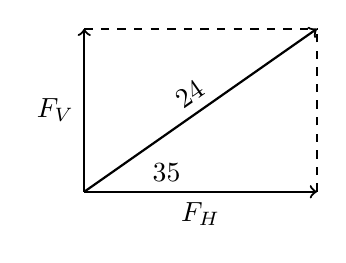
\begin{tikzpicture}[scale=1.5]
        \draw[thick,->] (0,0) -- (0,1.38) node[pos=0.5,anchor=east] {$F_V$};
        \draw[thick,->] (0,0) -- (1.97,0) node[pos=0.5,anchor=north] {$F_H$} node[pos=0.25,anchor=south west] {\ang{35}};
        \draw[thick,dashed] (0,1.38) -- (1.97,1.38);
        \draw[thick,dashed] (1.97,0) -- (1.97,1.38);
        \draw[thick,->] (0,0) -- (1.97,1.38) node[pos=0.5,anchor=south,rotate=35] {\SI{24}{\newton}};
    \end{tikzpicture}
    \end{center}
    What are the magnitudes of the horizontal and vertical components?
    \begin{choices}
        \wrongchoice{$F_H=\SI{3.5}{\newton}$ and $F_V=\SI{4.9}{\newton}$}
        \wrongchoice{$F_H=\SI{4.9}{\newton}$ and $F_V=\SI{3.5}{\newton}$}
        \wrongchoice{$F_H=\SI{14}{\newton}$ and $F_V=\SI{20.}{\newton}$}
      \correctchoice{$F_H=\SI{20.}{\newton}$ and $F_V=\SI{14}{\newton}$}
    \end{choices}
\end{question}
}


%% Section June2008
%%--------------------
\element{nysed}{
\begin{question}{June2008-Q01}
    The speedometer in a car does \emph{not} measure the car's velocity because velocity is a:
    \begin{choices}
      \correctchoice{vector quantity and has a direction associated with it}
        \wrongchoice{vector quantity and does not have a direction associated with it}
        \wrongchoice{scalar quantity and has a direction associated with it}
        \wrongchoice{scalar quantity and does not has a direction associated with it}
    \end{choices}
\end{question}
}

\element{nysed}{
\begin{question}{June2008-Q11}
    An airplane flies with a velocity of \SI{750}{\kilo\meter\per\hour},
        \ang{30} south of east.
    What is the magnitude of the eastward component of the plane's velocity?
    \begin{multicols}{2}
    \begin{choices}
        \wrongchoice{\SI{866}{\kilo\meter\per\hour}}
      \correctchoice{\SI{650}{\kilo\meter\per\hour}}
        \wrongchoice{\SI{433}{\kilo\meter\per\hour}}
        \wrongchoice{\SI{375}{\kilo\meter\per\hour}}
    \end{choices}
    \end{multicols}
\end{question}
}

\element{nysed}{
\begin{question}{June2008-Q41}
    The diagram below represents two concurrent forces.
    \begin{center}
    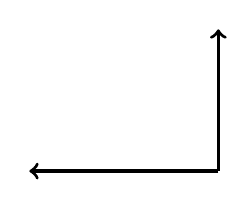
\begin{tikzpicture}[scale=0.60]
        \draw[very thick,->] (0,0) -- (0,3);
        \draw[very thick,->] (0,0) -- (-4,0);
    \end{tikzpicture}
    \end{center}
    Which vector represents the force that will produce equilibrium with these two forces?
    \begin{multicols}{2}
    \begin{choices}
        \AMCboxDimensions{down=-0.9cm}
        \wrongchoice{
            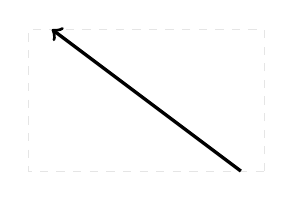
\begin{tikzpicture}[scale=0.60]
                \draw[dashed,white!90!black] (0.5,0) rectangle (-4.5,3);
                \draw[very thick,->] (0,0) -- (-4,3);
            \end{tikzpicture}
        }
        \wrongchoice{
            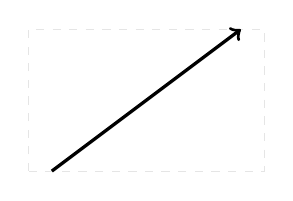
\begin{tikzpicture}[scale=0.60]
                \draw[dashed,white!90!black] (-0.5,0) rectangle (4.5,3);
                \draw[very thick,->] (0,0) -- (4,3);
            \end{tikzpicture}
        }
        %% ANS is 3
        \correctchoice{
            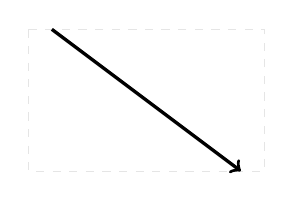
\begin{tikzpicture}[scale=0.60]
                \draw[dashed,white!90!black] (-0.5,0) rectangle (4.5,-3);
                \draw[very thick,->] (0,0) -- (4,-3);
            \end{tikzpicture}
        }
        \wrongchoice{
            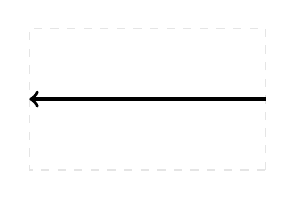
\begin{tikzpicture}[scale=0.60]
                \draw[dashed,white!90!black] (0,-1.5) rectangle (-5,1.5);
                \draw[very thick,->] (0,0) -- (-5,0);
            \end{tikzpicture}
        }
    \end{choices}
    \end{multicols}
\end{question}
}


%% Section Jan2008
%%--------------------
\element{nysed}{
\begin{question}{Jan2008-Q01}
    Which is a vector quantity?
    \begin{multicols}{2}
    \begin{choices}
        \wrongchoice{speed}
        \wrongchoice{mass}
        \wrongchoice{work}
      \correctchoice{displacement}
    \end{choices}
    \end{multicols}
\end{question}
}

\element{nysed}{
\begin{question}{Jan2008-Q04}
    A soccer player kicks a ball with an initial velocity
        of \SI{10}{\meter\per\second} at an angle of
        \ang{30} above the horizontal.
    The magnitude of the horizontal component of the ball's
        initial velocity is:
    \begin{multicols}{2}
    \begin{choices}
      \correctchoice{\SI{8.7}{\meter\per\second}}
        \wrongchoice{\SI{5.0}{\meter\per\second}}
        \wrongchoice{\SI{9.8}{\meter\per\second}}
        \wrongchoice{\SI{10}{\meter\per\second}}
    \end{choices}
    \end{multicols}
\end{question}
}

\element{nysed}{
\begin{question}{Jan2008-Q38}
    Two forces act concurrently on an object.
    Their resultant force has the largest magnitude when
        the angle between the forces is:
    \begin{multicols}{2}
    \begin{choices}
      \correctchoice{\ang{0}}
        \wrongchoice{\ang{90}}
        \wrongchoice{\ang{30}}
        \wrongchoice{\ang{180}}
    \end{choices}
    \end{multicols}
\end{question}
}


%% Section June2007
%%--------------------
\element{nysed}{
\begin{question}{June2007-Q05}
    As the angle between two concurrent forces decreases,
        the magnitude of the force required to produce equilibrium
    \begin{multicols}{2}
    \begin{choices}
        \wrongchoice{decreases}
      \correctchoice{increases}
        \wrongchoice{remains the same}
    \end{choices}
    \end{multicols}
\end{question}
}

\element{nysed}{
\begin{question}{June2007-Q06}
    A child walks \SI{5.0}{\meter} north, then \SI{4.0}{\meter} east,
        and finally \SI{2.0}{\meter} south.
    What is the magnitude of the resultant displacement of the child after
        the entire walk?
    \begin{multicols}{2}
    \begin{choices}
      \correctchoice{\SI{5.0}{\meter}}
        \wrongchoice{\SI{1.0}{\meter}}
        \wrongchoice{\SI{3.0}{\meter}}
        \wrongchoice{\SI{11.0}{\meter}}
    \end{choices}
    \end{multicols}
\end{question}
}

\element{nysed}{
\begin{question}{June2007-Q38}
    A stream is \SI{30}{\meter} wide and it current flows southward at
        \SI{1.5}{\meter\per\second}.
    A toy boat is launched with a velocity of
        \SI{2.0}{\meter\per\second} eastward from the west bank of the stream.
    What is the magnitude of the boat's resultant velocity as it crossed the stream?
    \begin{multicols}{2}
    \begin{choices}
        \wrongchoice{\SI{0.5}{\meter\per\second}}
      \correctchoice{\SI{2.5}{\meter\per\second}}
        \wrongchoice{\SI{3.0}{\meter\per\second}}
        \wrongchoice{\SI{3.5}{\meter\per\second}}
    \end{choices}
    \end{multicols}
\end{question}
}

\element{nysed}{
\begin{question}{June2007-Q39}
    A stream is \SI{30}{\meter} wide and it current flows southward at
        \SI{1.5}{\meter\per\second}.
    A toy boat is launched with a velocity of \SI{2.0}{\meter\per\second}
        eastward from the west bank of the stream.
    How much time is required for the boat to reach the opposite
        bank of the stream?
    \begin{multicols}{2}
    \begin{choices}
        \wrongchoice{\SI{8.6}{\second}}
        \wrongchoice{\SI{12}{\second}}
      \correctchoice{\SI{15}{\second}}
        \wrongchoice{\SI{60}{\second}}
    \end{choices}
    \end{multicols}
\end{question}
}

%% Section Jan2007
%%--------------------
\element{nysed}{
\begin{question}{Jan2007-Q02}
    A \SI{6.0}{\newton} force and an \SI{8.0}{\newton} force act
        concurrently on a point.
    As the angle between these forces increases from \ang{0} to \ang{90},
        the magnitude of their resultant:
    \begin{choices}
      \correctchoice{decreases}
        \wrongchoice{increases}
        \wrongchoice{remains the same}
    \end{choices}
\end{question}
}


%% Section June2006
%%--------------------
\element{nysed}{
\begin{question}{June2006-Q03}
    The diagram below represents a force vector, $A$, and a
        resultant vector, $R$.
    \begin{center}
        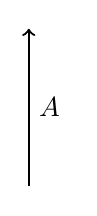
\begin{tikzpicture}
            \draw[thick,->] (0,0) -- (0,2cm);
            \node[thick,anchor=west] at (0,1cm) {$A$};
        \end{tikzpicture}
        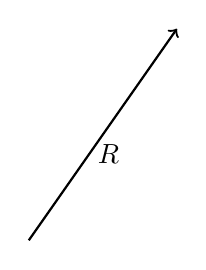
\begin{tikzpicture}
            \draw[thick,->] (0,0) -- (55:3.28cm);
            \node[thick,anchor=north,xshift=2pt] at (55:1.64cm) {$R$};
        \end{tikzpicture}
    \end{center}
    Which force vector $B$ below could be added to force vector
        $A$ to produce resultant vector $R$?
    \begin{multicols}{2}
    \begin{choices}
        \AMCboxDimensions{down=-1.0em}
        \correctchoice{
            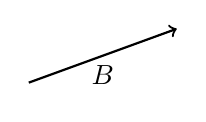
\begin{tikzpicture}
                \draw[thick,->] (0,0) -- (20:2cm);
                \node[thick,anchor=north] at (20:1cm) {$B$};
            \end{tikzpicture}
        }
        \wrongchoice{
            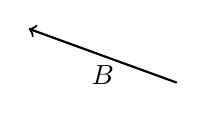
\begin{tikzpicture}
                \draw[thick,->] (0,0) -- (160:2cm);
                \node[thick,anchor=north] at (160:1cm) {$B$};
            \end{tikzpicture}
        }
        \wrongchoice{
            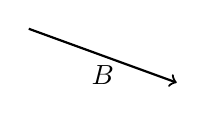
\begin{tikzpicture}
                \draw[thick,->] (0,0) -- (-20:2cm);
                \node[thick,anchor=north] at (-20:1cm) {$B$};
            \end{tikzpicture}
        }
        \wrongchoice{
            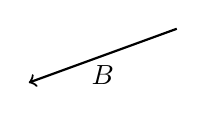
\begin{tikzpicture}
                \draw[thick,->] (0,0) -- (200:2cm);
                \node[thick,anchor=north] at (200:1cm) {$B$};
            \end{tikzpicture}
        }
    \end{choices}
    \end{multicols}
\end{question}
}

\element{nysed}{
\begin{question}{June2006-Q04}
    A golf ball is propelled with an initial velocity of
        \SI{60}{\meter\per\second} at \ang{37} above the horizontal.
    The horizontal component of the golf ball's initial velocity is:
    \begin{multicols}{2}
    \begin{choices}
      \correctchoice{\SI{48}{\meter\per\second}}
        \wrongchoice{\SI{40}{\meter\per\second}}
        \wrongchoice{\SI{30}{\meter\per\second}}
        \wrongchoice{\SI{36}{\meter\per\second}}
    \end{choices}
    \end{multicols}
\end{question}
}

\element{nysed}{
\begin{question}{June2006-Q06}
    A \SI{3}{\newton} force and a \SI{4}{\newton} force are acting concurrently on a point.
    Which force could not produce equilibrium with these two forces?
    \begin{multicols}{2}
    \begin{choices}
        \wrongchoice{\SI{1}{\newton}}
        \wrongchoice{\SI{7}{\newton}}
      \correctchoice{\SI{9}{\newton}}
        \wrongchoice{\SI{4}{\newton}}
    \end{choices}
    \end{multicols}
\end{question}
}


%% Section Jan2006
%%--------------------
\element{nysed}{
\begin{question}{Jan2006-Q04}
    A projectile is fired with an initial velocity of
        \SI{120}{\meter\per\second}
        at an angle, $\theta$, above the horizontal.
    If the projectile's initial horizontal speed is
        \SI{55}{\meter\per\second}, then angle $\theta$
        measures approximately:
    \begin{multicols}{4}
    \begin{choices}
      \correctchoice{\ang{63}}
        \wrongchoice{\ang{75}}
        \wrongchoice{\ang{27}}
        \wrongchoice{\ang{13}}
    \end{choices}
    \end{multicols}
\end{question}
}

\element{nysed}{
\begin{question}{Jan2006-Q03}
    Which is a scalar quantity?
    \begin{multicols}{2}
    \begin{choices}
      \correctchoice{speed}
        \wrongchoice{acceleration}
        \wrongchoice{displacement}
        \wrongchoice{momentum}
    \end{choices}
    \end{multicols}
\end{question}
}

\element{nysed}{
\begin{question}{Jan2006-Q12}
    A student on her way to school walks four blocks east,
        three block north, and another four blocks east,
        as shown in the diagram.
    \begin{center}
        \includegraphics[keepaspectratio,width=\linewidth]{Jan2006-Q12}
    \end{center}
    Compared to the distance she walks,
        the magnitude of her displacement home to school is:
    \begin{multicols}{3}
    \begin{choices}
      \correctchoice{less}
        \wrongchoice{more}
        \wrongchoice{the same}
    \end{choices}
    \end{multicols}
\end{question}
}

\element{nysed}{
\begin{question}{Jan2006-Q46}
    Two \SI{30}{\newton} forces act concurrently on an object.
    In which diagram would the forces produce a
        resultant with a magnitude of \SI{30}{\newton}?
    \begin{multicols}{2}
    \begin{choices}
        \AMCboxDimensions{down=-1.0em}
        \correctchoice{
            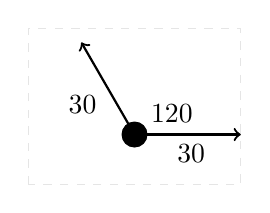
\begin{tikzpicture}[scale=0.9]
                \draw[dashed,white!90!black] (-1.5cm,-2em) rectangle (1.5cm,1.5cm);
                \draw[fill] (0,0) circle [radius=0.5em];
                \node[anchor=south west] at (15:0.1cm) {\ang{120}};
                \draw[thick,->] (0,0) -- (0:1.5cm);
                \node[anchor=north] at (0:0.8cm) {\SI{30}{\newton}};
                \draw[thick,->] (0,0) -- (120:1.5cm);
                \node[anchor=north east] at (120:0.8cm) {\SI{30}{\newton}};
            \end{tikzpicture}
        }
        \wrongchoice{
            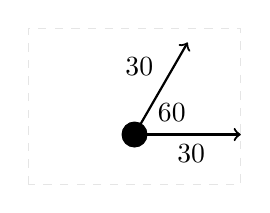
\begin{tikzpicture}[scale=0.9]
                \draw[dashed,white!90!black] (-1.5cm,-2em) rectangle (1.5cm,1.5cm);
                \draw[fill] (0,0) circle [radius=0.5em];
                \node[anchor=south west] at (15:0.2cm) {\ang{60}};
                \draw[thick,->] (0,0) -- (0:1.5cm);
                \node[anchor=north] at (0:0.8cm) {\SI{30}{\newton}};
                \draw[thick,->] (0,0) -- (60:1.5cm);
                \node[anchor=south east] at (60:0.8cm) {\SI{30}{\newton}};
            \end{tikzpicture}
        }
        \wrongchoice{
            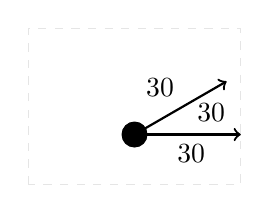
\begin{tikzpicture}[scale=0.9]
                \draw[dashed,white!90!black] (-1.5cm,-2em) rectangle (1.5cm,1.5cm);
                \draw[fill] (0,0) circle [radius=0.5em];
                \node[anchor=south west] at (4:0.75cm) {\ang{30}};
                \draw[thick,->] (0,0) -- (0:1.5cm);
                \node[anchor=north] at (0:0.8cm) {\SI{30}{\newton}};
                \draw[thick,->] (0,0) -- (30:1.5cm);
                \node[anchor=south east] at (30:0.8cm) {\SI{30}{\newton}};
            \end{tikzpicture}
        }
        \wrongchoice{
            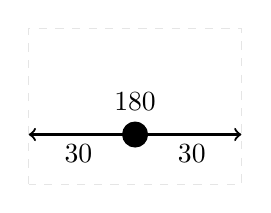
\begin{tikzpicture}[scale=0.9]
                \draw[dashed,white!90!black] (-1.5cm,-2em) rectangle (1.5cm,1.5cm);
                \draw[fill] (0,0) circle [radius=0.5em];
                \node[anchor=south] at (90:0.2cm) {\ang{180}};
                \draw[thick,->] (0,0) -- (0:1.5cm);
                \node[anchor=north] at (0:0.8cm) {\SI{30}{\newton}};
                \draw[thick,->] (0,0) -- (180:1.5cm);
                \node[anchor=north] at (180:0.8cm) {\SI{30}{\newton}};
            \end{tikzpicture}
        }
    \end{choices}
    \end{multicols}
\end{question}
}


%% Section June2005
%%--------------------
\element{nysed}{
\begin{question}{June2005-Q03}
    A \SI{5.0}{\newton} force and a \SI{7.0}{\newton} force act concurrently on a point.
    As the angle between the forces is increased from \ang{0} to \ang{180},
        the magnitude of the resultant of the two forces changes from:
    \begin{multicols}{2}
    \begin{choices}
      \correctchoice{\SI{12.0}{\newton} to \SI{2.0}{\newton}}
        \wrongchoice{\SI{0.0}{\newton} to \SI{12.0}{\newton}}
        \wrongchoice{\SI{2.0}{\newton} to \SI{12.0}{\newton}}
        \wrongchoice{\SI{12.0}{\newton} to \SI{0.0}{\newton}}
    \end{choices}
    \end{multicols}
\end{question}
}

\element{nysed}{
\begin{question}{June2005-Q04}
    A \SI{5.0}{\newton} force could have perpendicular components of:
    \begin{multicols}{2}
    \begin{choices}
      \correctchoice{\SI{3.0}{\newton} and \SI{4.0}{\newton}}
        \wrongchoice{\SI{1.0}{\newton} and \SI{4.0}{\newton}}
        \wrongchoice{\SI{2.0}{\newton} and \SI{3.0}{\newton}}
        \wrongchoice{\SI{5.0}{\newton} and \SI{5.0}{\newton}}
    \end{choices}
    \end{multicols}
\end{question}
}


%% Section Jan2005
%%--------------------
\element{nysed}{
\begin{question}{Jan2005-Q03}
    A golf ball is hit with an initial velocity of \SI{15}{\meter\per\second} at an angle of \ang{35} above the horizontal.
    What is the vertical component of the gold ball's initial velocity?
    \begin{multicols}{2}
    \begin{choices}
      \correctchoice{\SI{8.6}{\meter\per\second}}
        \wrongchoice{\SI{9.8}{\meter\per\second}}
        \wrongchoice{\SI{12}{\meter\per\second}}
        \wrongchoice{\SI{15}{\meter\per\second}}
    \end{choices}
    \end{multicols}
\end{question}
}

\element{nysed}{
\begin{question}{Jan2005-Q37}
    The vector below represents two forces, $F_1$ and $F_2$, simultaneously acting on an object.
    \begin{center}
    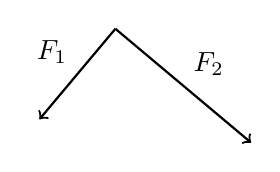
\begin{tikzpicture}[scale=0.75]
        \draw[thick,->] (0,0) -- (230:2cm)
            node[pos=0.5,anchor=south east] {$F_1$};
        \draw[thick,->] (0,0) -- (320:3cm)
            node[pos=0.5,anchor=south west] {$F_2$};
    \end{tikzpicture}
    \end{center}
    Which vector best represents the resultant of the two forces?
    \begin{multicols}{2}
    \begin{choices}
        \AMCboxDimensions{down=-1.5em}
        \correctchoice{
            \begin{tikzpicture}[scale=0.75]
                \draw[dashed,white!90!black] (-1.00,-3.5) rectangle (2.50,0);
                \draw[thick,->] (0,0) -- (286:3.6cm)
                    node[pos=0.5,anchor=east] {$R$};
            \end{tikzpicture}
        }
        \wrongchoice{
            \begin{tikzpicture}[scale=0.75]
                \draw[dashed,white!90!black] (+1.00,+3.5) rectangle (-2.50,-0);
                \draw[thick,->] (0,0) -- (106:3.6cm)
                    node[pos=0.5,anchor=east] {$R$};
            \end{tikzpicture}
        }
        \wrongchoice{
            \begin{tikzpicture}[scale=0.75]
                \draw[dashed,white!90!black] (+0.25,+2) rectangle (-3.75,-1.5);
                \draw[thick,->] (0,0) -- (176:3.6cm)
                    node[pos=0.5,anchor=south west] {$R$};
            \end{tikzpicture}
        }
        \wrongchoice{
            \begin{tikzpicture}[scale=0.75]
                \draw[dashed,white!90!black] (-0.25,-2) rectangle (3.75,1.5);
                \draw[thick,->] (0,0) -- (356:3.6cm)
                    node[pos=0.5,anchor=south west] {$R$};
            \end{tikzpicture}
        }
    \end{choices}
    \end{multicols}
\end{question}
}


%% Section June2004
%%--------------------
\element{nysed}{
\begin{question}{June2004-Q01}
    Velocity is to speed as displacement is to:
    \begin{multicols}{2}
    \begin{choices}
      \correctchoice{distance}
        \wrongchoice{acceleration}
        \wrongchoice{time}
        \wrongchoice{momentum}
    \end{choices}
    \end{multicols}
\end{question}
}

\element{nysed}{
\begin{question}{June2004-Q02}
    The diagram below shows a resultant vector, $R$.
    \begin{center}
    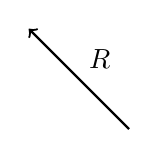
\begin{tikzpicture}[scale=0.9]
        \draw[thick,->] (0,0) -- (135:2cm)
            node[pos=0.5,anchor=south west] {$R$};
    \end{tikzpicture}
    \end{center}
    Which diagram best represents a pair of component vectors, $A$ and $B$,
        that would combine to form resultant vector $R$?
    \begin{multicols}{2}
    \begin{choices}
        \AMCboxDimensions{down=-0.5cm}
        \correctchoice{
            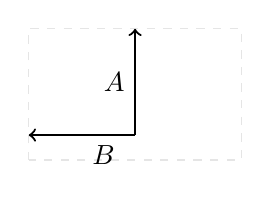
\begin{tikzpicture}[scale=0.9]
                \draw[dashed,white!90!black] (-1.5cm,-1em) rectangle (1.5cm,1.5cm);
                \draw[thick,->] (0,0) -- (90:1.5cm)
                    node[pos=0.5,anchor=east] {$A$};
                \draw[thick,->] (0,0) -- (180:1.5cm)
                    node[pos=0.5,anchor=north west] {$B$};
            \end{tikzpicture}
        }
        \wrongchoice{
            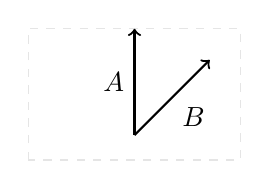
\begin{tikzpicture}[scale=0.9]
                \draw[dashed,white!90!black] (-1.5cm,-1em) rectangle (1.5cm,1.5cm);
                \draw[thick,->] (0,0) -- (90:1.5cm)
                    node[pos=0.5,anchor=east] {$A$};
                \draw[thick,->] (0,0) -- (45:1.5cm)
                    node[pos=0.5,anchor=north west] {$B$};
            \end{tikzpicture}
        }
        \wrongchoice{
            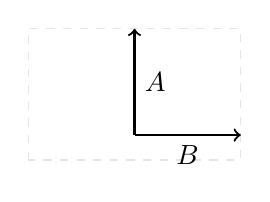
\begin{tikzpicture}[scale=0.9]
                \draw[dashed,white!90!black] (-1.5cm,-1em) rectangle (1.5cm,1.5cm);
                \draw[thick,->] (0,0) -- (90:1.5cm)
                    node[pos=0.5,anchor=west] {$A$};
                \draw[thick,->] (0,0) -- (0:1.5cm)
                    node[pos=0.5,anchor=north] {$B$};
            \end{tikzpicture}
        }
        \wrongchoice{
            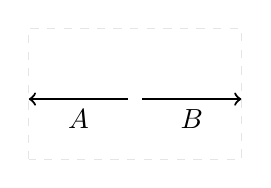
\begin{tikzpicture}[scale=0.9]
                \draw[dashed,white!90!black] (-1.5cm,-1em-0.50cm) rectangle (1.5cm,1.00cm);
                \draw[thick,->] (-0.1cm,0) -- (180:1.5cm)
                    node[pos=0.5,anchor=north] {$A$};
                \draw[thick,->] (0.1cm,0) -- (0:1.5cm)
                    node[pos=0.5,anchor=north] {$B$};
            \end{tikzpicture}
        }
    \end{choices}
    \end{multicols}
\end{question}
}


%% Section Jan2004
%%--------------------
\element{nysed}{
\begin{question}{Jan2004-Q01}
    A girl leaves a history classroom and walks \SI{10}{\meter} north to a drinking fountain.
    Then she turns and walks \SI{30}{\meter} south to an art classroom.
    What is the girl's total displacement from the history classroom to the art classroom?
    \begin{multicols}{2}
    \begin{choices}
      \correctchoice{\SI{20.}{\meter} south}
        \wrongchoice{\SI{20.}{\meter} north}
        \wrongchoice{\SI{40.}{\meter} south}
        \wrongchoice{\SI{40.}{\meter} north}
    \end{choices}
    \end{multicols}
\end{question}
}

\element{nysed}{
\begin{question}{Jan2004-Q02}
    One car travels \SI{40}{\meter} due east in \SI{5.0}{\second},
        and a second car travels \SI{64}{\meter} due west in \SI{8.0}{\second}.
    During their periods of travel, the cars definitely had the same
    \begin{choices}
      \correctchoice{average speed}
        \wrongchoice{average velocity}
        \wrongchoice{total displacement}
        \wrongchoice{change in momentum}
    \end{choices}
\end{question}
}

\element{nysed}{
\begin{question}{Jan2004-Q39}
    The diagram below represents a \SI{5.0}{\newton} force and a \SI{12}{\newton} force acting on point $P$.
    \begin{center}
    \begin{tikzpicture}
        \node[anchor=north east] at (0:0) {$P$};
        \draw[fill] (0,0) circle [radius=2pt];
        \draw[thick,->] (0,0) -- (90:2cm);
        \node[anchor=south,rotate=90] at (90:1cm) {\SI{5}{\newton}};
        \draw[thick,->] (0,0) -- (0:4.8cm);
        \node[anchor=north] at (0:2.4cm) {\SI{12}{\newton}};
    \end{tikzpicture}
    \end{center}
    The resultant of the two forces has magnitude of:
    \begin{multicols}{2}
    \begin{choices}
      \correctchoice{\SI{13}{\newton}}
        \wrongchoice{\SI{12}{\newton}}
        \wrongchoice{\SI{5.0}{\newton}}
        \wrongchoice{\SI{7.0}{\newton}}
    \end{choices}
    \end{multicols}
\end{question}
}


%% Section June2003
%%--------------------
\element{nysed}{
\begin{question}{June2003-Q02}
    A vector makes an angle $\theta$ with the horizontal.
    The horizontal and vertical components of the vector will be equal in magnitude if angle $\theta$ is:
    \begin{multicols}{4}
    \begin{choices}
      \correctchoice{\ang{45}}
        \wrongchoice{\ang{30}}
        \wrongchoice{\ang{60}}
        \wrongchoice{\ang{90}}
    \end{choices}
    \end{multicols}
\end{question}
}

\element{nysed}{
\begin{question}{June2003-Q36}
    Force $A$ and $B$ have a resultant $R$. 
    Force $A$ and resultant $R$ are represented in the diagram below.
    \begin{center}
    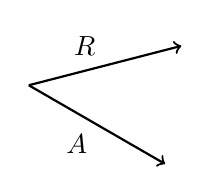
\begin{tikzpicture}
        \draw[thick,->] (0,0) -- (14.47:2cm);
        \node[anchor=south east] at (14.47:1cm) {$R$};
        \draw[thick,->] (0,0) -- (-30:2cm);
        \node[anchor=north east] at (-30:1cm) {$A$};
    \end{tikzpicture}
    \end{center}
    Which vector best represents force $B$?
    \begin{multicols}{2}
    \begin{choices}
        \AMCboxDimensions{down=-0.5cm}
        \correctchoice{
            \begin{tikzpicture}
                \draw[draw=white] (-0.75,0) rectangle (0.75,1);
                \draw[thick,->] (0,0) -- (90:1cm)
                    node[pos=0.5,anchor=east] {$B$};
            \end{tikzpicture}
        }
        \wrongchoice{
            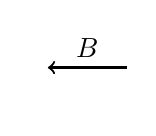
\begin{tikzpicture}
                \draw[draw=white] (-0.25,-0.5) rectangle (-1.25,0.5);
                \draw[thick,->] (0,0) -- (180:1cm)
                    node[pos=0.5,anchor=south] {$B$};
            \end{tikzpicture}
        }
        \wrongchoice{
            \begin{tikzpicture}
                \draw[draw=white] (-0.75,0) rectangle (0.75,-1);
                \draw[thick,->] (0,0) -- (270:1cm)
                    node[pos=0.5,anchor=east] {$B$};
            \end{tikzpicture}
        }
        \wrongchoice{
            \begin{tikzpicture}
                \draw[draw=white] (-0.25,-0.5) rectangle (1.25,0.5);
                \draw[thick,->] (0,0) -- (0:1cm)
                    node[pos=0.5,anchor=south] {$B$};
            \end{tikzpicture}
        }
    \end{choices}
    \end{multicols}
\end{question}
}


%% Section Jan2003
%%--------------------
\element{nysed}{
\begin{question}{Jan2003-Q02}
    A car travels \SI{90}{\meter} due north in \SI{15}{\second}.
    Then the car turns around and travels \SI{40}{\meter} due south in \SI{5.0}{\second}.
    What is the magnitude of the average velocity of the car during this \SI{20}{\second} interval?
    \begin{multicols}{2}
    \begin{choices}
      \correctchoice{\SI{2.5}{\meter\per\second}}
        \wrongchoice{\SI{5.0}{\meter\per\second}}
        \wrongchoice{\SI{6.5}{\meter\per\second}}
        \wrongchoice{\SI{7.0}{\meter\per\second}}
    \end{choices}
    \end{multicols}
\end{question}
}

\element{nysed}{
\begin{question}{Jan2003-Q36}
    Which pair of forces acting concurrently on an object will produce the resultant of greatest magnitude?
    \begin{multicols}{2}
    \begin{choices}
        \AMCboxDimensions{down=-0.5em}
        \correctchoice{
            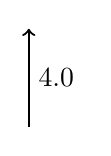
\begin{tikzpicture}
                \draw[thick,->] (0,0) -- (90:1.25cm);
                \node[anchor=west] at (90:0.625cm) {\SI{4.0}{\newton}};
            \end{tikzpicture}
            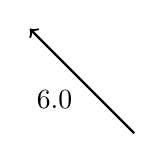
\begin{tikzpicture}
                \draw[thick,->] (0,0) -- (135:1.875cm);
                \node[anchor=north east] at (135:0.9375cm) {\SI{6.0}{\newton}};
            \end{tikzpicture}
        }
        \wrongchoice{
            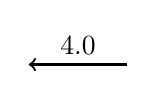
\begin{tikzpicture}
                \draw[thick,->] (0,0) -- (180:1.25cm);
                \node[anchor=south] at (180:0.625cm) {\SI{4.0}{\newton}};
            \end{tikzpicture}
            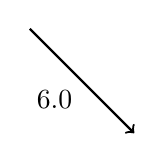
\begin{tikzpicture}
                \draw[thick,->] (0,0) -- (-45:1.875cm);
                \node[anchor=north east] at (-45:0.9375cm) {\SI{6.0}{\newton}};
            \end{tikzpicture}
        }
        \wrongchoice{
            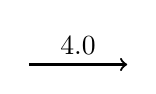
\begin{tikzpicture}
                \draw[thick,->] (0,0) -- (0:1.25cm);
                \node[anchor=south] at (0:0.625cm) {\SI{4.0}{\newton}};
            \end{tikzpicture}
            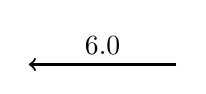
\begin{tikzpicture}
                \draw[thick,->] (0,0) -- (180:1.875cm);
                \node[anchor=south] at (180:0.9375cm) {\SI{6.0}{\newton}};
            \end{tikzpicture}
        }
        \wrongchoice{
            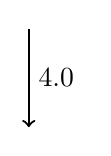
\begin{tikzpicture}
                \draw[thick,->] (0,0) -- (270:1.25cm);
                \node[anchor=west] at (270:0.625cm) {\SI{4.0}{\newton}};
            \end{tikzpicture}
            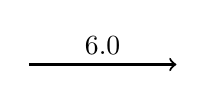
\begin{tikzpicture}
                \draw[thick,->] (0,0) -- (0:1.875cm);
                \node[anchor=south] at (0:0.9375cm) {\SI{6.0}{\newton}};
            \end{tikzpicture}
        }
    \end{choices}
    \end{multicols}
\end{question}
}


%% Section Aug2002
%%--------------------
\element{nysed}{
\begin{question}{Aug2002-Q07}
    Which term represents a scalar quantity?
    \begin{multicols}{2}
    \begin{choices}
      \correctchoice{distance}
        \wrongchoice{displacement}
        \wrongchoice{force}
        \wrongchoice{weight}
    \end{choices}
    \end{multicols}
\end{question}
}

\element{nysed}{
\begin{question}{Aug2002-Q40}
    Which vector diagram represents the greatest magnitude of displacement for an object?
    \begin{multicols}{2}
    \begin{choices}
        \AMCboxDimensions{down=-1.3cm}
        \wrongchoice{
            \begin{tikzpicture}[scale=2]
                \draw[dashed,white!90!black] (-1.3,-0.4) rectangle (0.3,1.3);
                \draw[very thick,->] (0,0) -- (0,1) node[pos=0.5,anchor=south,rotate=-90] {\SI{1}{\meter}};
            \end{tikzpicture}
        }
        \correctchoice{
            \begin{tikzpicture}[scale=2]
                \draw[dashed,white!90!black] (-1.3,-0.4) rectangle (0.3,1.3);
                \draw[very thick,->] (0,0) -- (0,1) node[pos=0.5,anchor=south,rotate=-90] {\SI{1}{\meter}};
                \draw[very thick,->] (0,1) -- (-1,1) node[pos=0.5,anchor=south] {\SI{1}{\meter}};
            \end{tikzpicture}
        }
        \wrongchoice{
            \begin{tikzpicture}[scale=2]
                \draw[dashed,white!90!black] (-1.3,-0.4) rectangle (0.3,1.3);
                \draw[very thick,->] (0,0) -- (0,1) node[pos=0.5,anchor=south,rotate=-90] {\SI{1}{\meter}};
                \draw[very thick,->] (0,1) -- (-1,1) node[pos=0.5,anchor=south] {\SI{1}{\meter}};
                \draw[very thick,->] (-1,1) -- (-1,0) node[pos=0.5,rotate=90,anchor=south] {\SI{1}{\meter}};
            \end{tikzpicture}
        }
        \wrongchoice{
            \begin{tikzpicture}[scale=2]
                \draw[dashed,white!90!black] (-1.3,-0.4) rectangle (0.3,1.3);
                \draw[very thick,->] (0,0) -- (0,1) node[pos=0.5,anchor=south,rotate=-90] {\SI{1}{\meter}};
                \draw[very thick,->] (0,1) -- (-1,1) node[pos=0.5,anchor=south] {\SI{1}{\meter}};
                \draw[very thick,->] (-1,1) -- (-1,0) node[pos=0.5,rotate=90,anchor=south] {\SI{1}{\meter}};
                \draw[very thick,->] (-1,0) -- (0,0) node[pos=0.5,anchor=south] {\SI{1}{\meter}};
            \end{tikzpicture}
        }
    \end{choices}
    \end{multicols}
\end{question}
}


%% Section June2002
%%--------------------
\element{nysed}{
\begin{question}{June2002-Q44}
    A force vector was resolved into two perpendicular components,
        $F_1$ and $F_2$, as shown in the diagram below.
    \begin{center}
    \begin{tikzpicture}
        \draw[thick,->] (0,0) -- (180:1.00cm);
        \node[anchor=south] at (180:0.5cm) {$F_1$};
        \draw[thick,->] (0,0) -- (270:1.50cm);
        \node[anchor=west] at (270:0.75cm) {$F_2$};
    \end{tikzpicture}
    \end{center}
    Which vector best represents the original force?
    \begin{multicols}{2}
    \begin{choices}
        \AMCboxDimensions{down=-1.0cm}
        \correctchoice{
            \begin{tikzpicture}
                \draw[dashed,white!90!black] (0.3,0.3) rectangle (-1.8,-1.8);
                \draw[thick,->] (0,0) -- (236:1.8cm)
                    node[pos=0.5,anchor=south east] {$R$};
            \end{tikzpicture}
        }
        \wrongchoice{
            \begin{tikzpicture}
                \draw[dashed,white!90!black] (-0.3,-0.3) rectangle (1.8,1.8);
                \draw[thick,->] (0,0) -- (56:1.8cm)
                    node[pos=0.5,anchor=north west] {$R$};
            \end{tikzpicture}
        }
        \wrongchoice{
            \begin{tikzpicture}
                \draw[dashed,white!90!black] (0.3,-0.3) rectangle (-1.8,1.8);
                \draw[thick,->] (0,0) -- (126:1.8cm)
                    node[pos=0.5,anchor=south west] {$R$};
            \end{tikzpicture}
        }
        \wrongchoice{
            \begin{tikzpicture}
                \draw[dashed,white!90!black] (-0.3,0.3) rectangle (1.8,-1.8);
                \draw[thick,->] (0,0) -- (306:1.8cm)
                    node[pos=0.5,anchor=north east] {$R$};
            \end{tikzpicture}
        }
    \end{choices}
    \end{multicols}
\end{question}
}


%% Section Jan2002
%%--------------------
\element{nysed}{
\begin{question}{Jan2002-Q01}
    What is the total displacement of a student who walks \num{3} blocks east,
        \num{2} blocks north, \num{1} block west,
        and then \num{2} blocks south?
    \begin{multicols}{2}
    \begin{choices}
        \wrongchoice{\num{0}}
      \correctchoice{\num{2} blocks east}
        \wrongchoice{\num{2} blocks west}
        \wrongchoice{\num{8} blocks}
    \end{choices}
    \end{multicols}
\end{question}
}

\element{nysed}{
\begin{question}{Jan2002-Q08}
    Two concurrent forces have a maximum resultant of \SI{45}{\newton} and a minimum resultant of \SI{5}{\newton}.
    What is the magnitude of each of these forces?
    \begin{multicols}{2}
    \begin{choices}
        \wrongchoice{\SI{0}{\newton} and \SI{45}{\newton}}
        \wrongchoice{\SI{5}{\newton} and \SI{9}{\newton}}
      \correctchoice{\SI{20}{\newton} and \SI{25}{\newton}}
        \wrongchoice{\SI{0}{\newton} and \SI{50}{\newton}}
    \end{choices}
    \end{multicols}
\end{question}
}


%% Section June2001
%%-------------------
\element{nysed}{
\begin{question}{June2001-Q01}
    Which terms both represents scalar quantities?
    \begin{choices}
        \wrongchoice{displacement and velocity}
      \correctchoice{distance and speed}
        \wrongchoice{displacement and speed}
        \wrongchoice{distance and velocity}
    \end{choices}
\end{question}
}

\element{nysed}{
\begin{question}{June2001-Q06}
    Two students push on a sled.
    One pushes with a force of \SI{30}{\newton} east and the other exerts a force of \SI{40}{\newton} south,
        as shown in the topview diagram below.
    \begin{center}
    \begin{tikzpicture}
        \draw (0,0) rectangle (1.5cm,1.0cm);
        \node[anchor=south,yshift=-3pt] at (0.75cm,0.50cm) {Top of};
        \node[anchor=north,yshift=3pt] at (0.75cm,0.50cm) {sled};
        \draw[thick,->] (0.75cm,0) -- (0.75cm,-1.2cm);
        \node[anchor=south west] at (0.75cm,-1.2cm) {\SI{40}{\newton} south};
        \draw[thick,->] (1.5cm,0.50cm) -- (2.4cm,0.50cm);
        \node[anchor=west] at (2.4cm,0.50cm) {\SI{30}{\newton} east};
    \end{tikzpicture}
    \end{center}
    Which vector best represents the resultant of these two forces?
    %% NOTE: I think the wrong direction should be 180 from correct
    \begin{multicols}{2}
    \begin{choices}
        \AMCboxDimensions{down=-0.5cm}
        \correctchoice{
            \begin{tikzpicture}
                \draw[draw=white] (0,0.3) rectangle (1.5,-1.2);
                \draw[thick,->] (0,0) -- (-45:1.5cm);
                \node[thick,anchor=south west] at (-45:0.75cm) {\SI{50}{\newton}};
            \end{tikzpicture}
        }
        \wrongchoice{
            \begin{tikzpicture}
                \draw[draw=white] (0,-0.3) rectangle (1.5,1.2);
                \draw[thick,->] (0,0) -- (45:1.5cm);
                \node[thick,anchor=north west] at (45:0.75cm) {\SI{50}{\newton}};
            \end{tikzpicture}
        }
        \wrongchoice{
            \begin{tikzpicture}
                \draw[draw=white] (0,0) rectangle (1.5,-1.5);
                \draw[thick,->] (0,0) -- (-45:2.1cm);
                \node[thick,anchor=south west] at (-45:1.05cm) {\SI{70}{\newton}};
            \end{tikzpicture}
        }
        \wrongchoice{
            \begin{tikzpicture}
                \draw[draw=white] (0,0) rectangle (1.5,1.5);
                \draw[thick,->] (0,0) -- (45:2.1cm);
                \node[thick,anchor=north west] at (45:1.05cm) {\SI{70}{\newton}};
            \end{tikzpicture}
        }
    \end{choices}
    \end{multicols}
\end{question}
}

\element{nysed}{
\begin{question}{June2001-Q56}
    A football player kicks a ball with an initial velocity of \SI{25}{\meter\per\second} at an angle of \ang{53} above the horizontal.
    The vertical component of the initial velocity of the ball is:
    \begin{multicols}{2}
    \begin{choices}
        \wrongchoice{\SI{25}{\meter\per\second}}
      \correctchoice{\SI{20}{\meter\per\second}}
        \wrongchoice{\SI{15}{\meter\per\second}}
        \wrongchoice{\SI{10}{\meter\per\second}}
    \end{choices}
    \end{multicols}
\end{question}
}


%% Section Jan2001
%%--------------------
\element{nysed}{
\begin{question}{Jan2001-Q03}
    The diagram below shows a block on a horizontal frictionless surface.
    A \SI{100}{\newton} force acts on the block at an angle of \ang{30} above the horizontal.
    \begin{center}
    \begin{tikzpicture}
        %% Unknown Force
        \draw[thick,->] (-1,0.5) -- (-3,0.5)
            node[pos=0.66,anchor=south] {$F$};
        %% Known Force
        \draw[dashed,thick,->] (1,0.5) -- (2.667,0.5)
            node[pos=0.5,anchor=south west] {\ang{30}};
        \draw[thick,->] (1,0.5) -- ++(30:3)
            node[pos=0.5,anchor=south,rotate=30] {\SI{100}{\newton}};
        %% Block
        \draw[thick] (-1,0) rectangle (1,1);
        \node[anchor=center] at (0,0.5) {Block};
        %% Floor
        \draw[thick] (-3.0,0) -- (3.0,0);
        \foreach \x in {-30,-29,...,30}
            \draw[thin] (\x mm,0cm) -- ++ (220:0.15cm);
        \node[anchor=north] at (0,-0.15) {Frictionless surface};
    \end{tikzpicture}
    \end{center}
    What is the magnitude of force $F$ if it establishes equilibrium?
    \begin{multicols}{2}
    \begin{choices}
        \wrongchoice{\SI{50.0}{\newton}}
        \wrongchoice{\SI{100}{\newton}}
      \correctchoice{\SI{86.6}{\newton}}
        \wrongchoice{\SI{187}{\newton}}
    \end{choices}
    \end{multicols}
\end{question}
}

\element{nysed}{
\begin{question}{Jan2001-Q05}
    A \SI{5}{\newton} force directed east and a \SI{5}{\newton} force directed north act concurrently on a point.
    The resultant of the two forces is:
    \begin{multicols}{2}
    \begin{choices}
        \wrongchoice{\SI{5.0}{\newton} northeast}
        \wrongchoice{\SI{10}{\newton} southwest}
      \correctchoice{\SI{7}{\newton} northeast}
        \wrongchoice{\SI{7}{\newton} southwest}
    \end{choices}
    \end{multicols}
\end{question}
}

\element{nysed}{
\begin{question}{Jan2001-Q06}
    Into how many possible components can a single force be resolved?
    \begin{choices}
        \wrongchoice{an unlimited number}
        \wrongchoice{two components}
      \correctchoice{three components}
        \wrongchoice{four components at right angles to each other}
    \end{choices}
\end{question}
}

\element{nysed}{
\begin{question}{Jan2001-Q63}
    A projectile is launched with an initial velocity of \SI{200}{\meter\per\second} at \ang{30} above the horizontal.
    What is the magnitude of the vertical component of the projectile's initial velocity?
    \begin{multicols}{2}
    \begin{choices}
        \wrongchoice{$\SI{200}{\meter\per\second} \times \cos{\ang{30}}$}
      \correctchoice{$\SI{200}{\meter\per\second} \times \sin{\ang{30}}$}
        \wrongchoice{$\dfrac{\SI{200}{\meter\per\second}}{\sin{\ang{30}}}$}
        \wrongchoice{$\dfrac{\SI{200}{\meter\per\second}}{\cos{\ang{30}}}$}
    \end{choices}
    \end{multicols}
\end{question}
}


%% Section June2000
%%--------------------
\element{nysed}{
\begin{question}{June2000-Q01}
    The map below shows the route traveled by a school bus.
    \begin{center}
        \includegraphics[keepaspectratio,width=\linewidth]{June2000-Q01}
    \end{center}
    What is the magnitude of the total displacement of the school bus from the start to the end of its trip?
    \begin{multicols}{2}
    \begin{choices}
        \wrongchoice{\SI{400}{\meter}}
        \wrongchoice{\SI{500}{\meter}}
      \correctchoice{\SI{800}{\meter}}
        \wrongchoice{\SI{1800}{\meter}}
    \end{choices}
    \end{multicols}
\end{question}
}

\element{nysed}{
\begin{question}{June2000-Q05}
    In the diagram below, a force, $F$, is applied to the handle of a lawnmower inclined at angle $\theta$ to the ground.
    \begin{center}
        \includegraphics[keepaspectratio,scale=1.0]{June2000-Q05}
    \end{center}
    The magnitude of the horizontal component of force $F$ depends on:
    \begin{choices}
        \wrongchoice{the magnitude of the force $F$, only}
        \wrongchoice{the measure of angle $\theta$, only}
      \correctchoice{both the magnitude of force $F$ and the measure of angle $\theta$.}
        \wrongchoice{neither the magnitude of force $F$ nor the measure of angle $\theta$.}
    \end{choices}
\end{question}
}


\element{nysed}{
\begin{question}{June2000-Q06}
    Equilibrium exists in a system where three forces are acting concurrently on an object.
    If the system includes a \SI{5.0}{\newton} force due north and a \SI{2.0}{\newton} force due south, the third force must be:
    \begin{multicols}{2}
    \begin{choices}
        \wrongchoice{\SI{7.0}{\newton} south}
        \wrongchoice{\SI{7.0}{\newton} north}
      \correctchoice{\SI{3.0}{\newton} south}
        \wrongchoice{\SI{3.0}{\newton} north}
    \end{choices}
    \end{multicols}
\end{question}
}

\element{nysed}{
\begin{question}{June2000-Q09}
    Which term represents a vector quantity and its respective unit?
    \begin{multicols}{2}
    \begin{choices}
        \wrongchoice{weight (\si{\kilo\gram})}
        \wrongchoice{mass (\si{\kilo\gram})}
      \correctchoice{force (\si{\newton})}
        \wrongchoice{momentum (\si{\newton})}
    \end{choices}
    \end{multicols}
\end{question}
}

\element{nysed}{
\begin{question}{June2000-Q10}
    The vector below represents the resultant of two forces acting concurrently on an object at point $P$.
    \begin{center}
    \begin{tikzpicture}
        \draw[fill] (0,0) circle [radius=2pt];
        \node[anchor=west] at (0,0) {$P$};
        \draw[thick,->] (0,0) -- (150:3.00cm);
        \node[anchor=south,rotate=-30] at (150:1.5cm) {Resultant};
    \end{tikzpicture}
    \end{center}
    Which pair of vectors best represents two concurrent forces that combine to produce this resultant force vector?
    \begin{multicols}{2}
    \begin{choices}
        \AMCboxDimensions{down=-1.0cm}
        \correctchoice{
            \begin{tikzpicture}[scale=0.75]
                \draw[draw=white] (-2cm,-1cm) rectangle (2cm,1cm);
                \draw[fill] (0,0) circle [radius=2pt];
                \node[anchor=north] at (0,0) {$P$};
                \draw[thick,->] (0,0) -- (0:1.5cm);
                \draw[thick,->] (0,0) -- (120:1.5cm);
            \end{tikzpicture}
        }
        \wrongchoice{
            \begin{tikzpicture}[scale=0.75]
                \draw[draw=white] (-2cm,-1cm) rectangle (2cm,1.3cm);
                \draw[fill] (0,0) circle [radius=2pt];
                \node[anchor=east] at (0,0) {$P$};
                \draw[thick,->] (0,0) -- (0:2cm);
                \draw[thick,->] (0,0) -- (90:1cm);
            \end{tikzpicture}
        }
        \wrongchoice{
            \begin{tikzpicture}[scale=0.75]
                \draw[draw=white] (-2cm,-1cm) rectangle (2cm,1cm);
                \draw[fill] (0,0) circle [radius=2pt];
                \node[anchor=south] at (0,0) {$P$};
                \draw[thick,->] (0,0) -- (180:2cm);
                \draw[thick,->] (0,0) -- (270:1cm);
            \end{tikzpicture}
        }
        \wrongchoice{
            \begin{tikzpicture}[scale=0.75]
                \draw[draw=white] (-2cm,-1cm) rectangle (2cm,1cm);
                \draw[fill] (0,0) circle [radius=2pt];
                \node[anchor=west] at (0,0) {$P$};
                \draw[thick,->] (0,0) -- (180:1.5cm);
                \draw[thick,->] (0,0) -- (120:1.5cm);
            \end{tikzpicture}
        }
    \end{choices}
    \end{multicols}
\end{question}
}


%% Section June1999
%%--------------------
\element{nysed}{
\begin{question}{June1999-Q01}
    A shown in the diagram below,
        a painter climbs \SI{7.3}{\meter} up a vertical scaffold from $A$ to $B$ and then walks \SI{11}{\meter} from $B$ to $C$ along a level platform.
    \begin{center}
        \includegraphics[keepaspectratio,scale=0.80]{June1999-Q01}
    \end{center}
    The magnitude of the painter's total displacement while moving from $A$ to $C$ is:
    \begin{multicols}{2}
    \begin{choices}
        \wrongchoice{\SI{3.7}{\meter}}
      \correctchoice{\SI{13.2}{\meter}}
        \wrongchoice{\SI{18.3}{\meter}}
        \wrongchoice{\SI{25.6}{\meter}}
    \end{choices}
    \end{multicols}
\end{question}
}

\element{nysed}{
\begin{question}{June1999-Q07}
    Which combination of three concurrent forces acting on a body could \emph{not} produce equilibrium?
    \begin{multicols}{2}
    \begin{choices}
      \correctchoice{\SI{1}{\newton},\SI{3}{\newton},\SI{5}{\newton}}
        \wrongchoice{\SI{2}{\newton},\SI{2}{\newton},\SI{2}{\newton}}
        \wrongchoice{\SI{3}{\newton},\SI{4}{\newton},\SI{5}{\newton}}
        \wrongchoice{\SI{4}{\newton},\SI{4}{\newton},\SI{5}{\newton}}
    \end{choices}
    \end{multicols}
\end{question}
}


%% Section June1998
%%--------------------
\element{nysed}{
\begin{question}{June1998-Q01}
    A car travels \SI{12}{\kilo\meter} due north and then \SI{8}{\kilo\meter} due west going from town $A$ to town $B$.
    What is the magnitude of the displacement of a helicopter that flies in a straight line from town $A$ to town $B$?
    \begin{multicols}{2}
    \begin{choices}
        \wrongchoice{\SI{20}{\kilo\meter}}
      \correctchoice{\SI{14}{\kilo\meter}}
        \wrongchoice{\SI{10}{\kilo\meter}}
        \wrongchoice{\SI{4}{\kilo\meter}}
    \end{choices}
    \end{multicols}
\end{question}
}

\element{nysed}{
\begin{question}{June1998-Q04}
    Forces $F_1$ and $F_2$ act concurrently on point $P$,
        as shown in the diagram below.
    \begin{center}
    \begin{tikzpicture}
        \draw[fill] (0,0) circle [radius=2pt];
        \node[anchor=north east] at (0,0) {$P$};

        \draw[thick,->] (0,0) -- (0:3.00cm);
        \node[anchor=north] at (0:1.50cm) {$F_2=\SI{10}{\newton}$ east};

        \draw[thick,->] (0,0) -- (90:3.00cm);
        \node[anchor=south,rotate=90] at (90:1.50cm) {$F_1=\SI{10}{\newton}$ north};
    \end{tikzpicture}
    \end{center}
    The equilibrant of $F_1$ and $F_2$ is:
    \begin{multicols}{2}
    \begin{choices}
      \correctchoice{\SI{14}{\newton} southwest}
        \wrongchoice{\SI{14}{\newton} southeast}
        \wrongchoice{\SI{20}{\newton} southwest}
        \wrongchoice{\SI{20}{\newton} southeast}
    \end{choices}
    \end{multicols}
\end{question}
}

\element{nysed}{
\begin{question}{June1998-Q61}
    An artillery shell is fired at an angle to the horizontal.
    Its initial velocity has a vertical component of \SI{150}{\meter\per\second} and a horizontal component of \SI{260}{\meter\per\second}.
    What is the magnitude of the initial velocity of the shell?
    \begin{multicols}{2}
    \begin{choices}
        \wrongchoice{\SI{9.0e4}{\meter\per\second}}
        \wrongchoice{\SI{4.1e2}{\meter\per\second}}
      \correctchoice{\SI{3.0e2}{\meter\per\second}}
        \wrongchoice{\SI{1.1e2}{\meter\per\second}}
    \end{choices}
    \end{multicols}
\end{question}
}


%% Section June1997
%%--------------------
\element{nysed}{
\begin{question}{June1997-Q01}
    What is the total displacement of a student who walks \num{3} blocks east,
        \num{2} blocks north, and \num{1} block west, and then \num{2} blocks south?
    \begin{multicols}{2}
    \begin{choices}
        \wrongchoice{\num{0}}
      \correctchoice{\num{2} blocks east}
        \wrongchoice{\num{2} blocks west}
        \wrongchoice{\num{8} blocks}
    \end{choices}
    \end{multicols}
\end{question}
}

\element{nysed}{
\begin{question}{June1997-Q08}
    A \SI{100}{\newton} force acts on point $P$,
        as shown in the diagram below.
    \begin{center}
    \begin{tikzpicture}
        \draw[fill] (0,0) circle [radius=2pt];
        \node[anchor=east] at (0,0) {$P$};
        \draw[thick,->] (0,0) -- (0:4.00cm);
        \node[anchor=north] at (0:2.00cm) {Horizontal};
        \draw[thick,->] (0,0) -- (30:4cm);
        \node[anchor=south,rotate=30] at (30:2cm) {\SI{100}{\newton}};
        \draw[thick,->] (0:2cm) arc (0:30:2cm);
        \node[anchor=south west] at (10:2cm) {\ang{30}};
    \end{tikzpicture}
    \end{center}
    The magnitude of the vertical component of this force is approximately:
    \begin{multicols}{2}
    \begin{choices}
        \wrongchoice{\SI{30}{\newton}}
      \correctchoice{\SI{50}{\newton}}
        \wrongchoice{\SI{71}{\newton}}
        \wrongchoice{\SI{87}{\newton}}
    \end{choices}
    \end{multicols}
\end{question}
}

\element{nysed}{
\begin{question}{June1997-Q61}
    A baseball player throws a baseball at a speed of
        \SI{40}{\meter\per\second} at an angle of
        \ang{30} to the ground.
    The horizontal component of the baseball's speed
        is approximately
    \begin{multicols}{2}
    \begin{choices}
        \wrongchoice{\SI{15}{\meter\per\second}}
        \wrongchoice{\SI{20}{\meter\per\second}}
        \wrongchoice{\SI{30}{\meter\per\second}}
      \correctchoice{\SI{35}{\meter\per\second}}
    \end{choices}
    \end{multicols}
\end{question}
}


%% Section June1996
%%--------------------
\element{nysed}{
\begin{question}{June1996-Q02}
    A student walks \SI{40}{\meter} along a hallway that heads due north,
        then turns and walks \SI{30}{\meter} along another hallway that heads due east.
    What is the magnitude of the student's resultant displacement?
    \begin{multicols}{2}
    \begin{choices}
        \wrongchoice{\SI{10}{\meter}}
        \wrongchoice{\SI{35}{\meter}}
      \correctchoice{\SI{50}{\meter}}
        \wrongchoice{\SI{70}{\meter}}
    \end{choices}
    \end{multicols}
\end{question}
}

\element{nysed}{
\begin{question}{June1996-Q08}
    Which pair of concurrent forces could produce a resultant force having a magnitude of \SI{10}{\newton}?
    \begin{multicols}{2}
    \begin{choices}
      \correctchoice{\SI{10}{\newton}, \SI{10}{\newton}}
        \wrongchoice{\SI{10}{\newton}, \SI{30}{\newton}}
        \wrongchoice{\SI{4.7}{\newton}, \SI{4.7}{\newton}}
        \wrongchoice{\SI{4.7}{\newton}, \SI{5.0}{\newton}}
    \end{choices}
    \end{multicols}
\end{question}
}


%% Section June1995
%%--------------------
\element{nysed}{
\begin{question}{June1995-Q06}
    A river flows due east at \SI{1.5}{\meter\per\second}.
    A motorboat leaves the north short of the river and heads due south at \SI{2.0}{\meter\per\second},
        as shown in the diagram below.
    \begin{center}
    \begin{tikzpicture}
        %% Banks
        \draw[ultra thick] (-3,+2) -- (+3,+2);
        \draw[ultra thick] (-3,-2) -- (+3,-2);
        %% Compass
        \node[circle,minimum size=4ex] (C) at (-3,0) {};
        \fill (C.west) to[out=20,in=160] (C.east) to[out=200,in=340] (C.west) -- cycle;
        \fill (C.north) to[out=290,in=70] (C.south) to[out=110,in=250] (C.north) -- cycle;
        %% Compass labels
        \node[anchor=west] at (C.east) {E};
        \node[anchor=east] at (C.west) {W};
        \node[anchor=south] at (C.north) {N};
        \node[anchor=north] at (C.south) {S};
        %% Boat
        \node[minimum size=0.5cm] (B) at (-1.5,1) {};
        \draw[fill=white!90!black] (B.south east) -- ++(225:0.3535) -- (B.south west) -- (B.north west) -- (B.north east) -- cycle;
        \draw[thick,->] (B.south) ++(270:0.25) -- ++(270:1.33)
            node[pos=0.5,anchor=west,text centered,text width=4em] {Boat \SI{2.0}{\meter\per\second}};
        %% Current
        \draw[thick,->] (1.5,0) -- ++(0:1) 
            node[pos=0.5,anchor=south,text centered,text width=4em] {River \SI{1.5}{\meter\per\second}};
    \end{tikzpicture}
    \end{center}
    Which vector best represents the resultant velocity of the boat relative to the riverbank?
    \begin{multicols}{2}
    \begin{choices}
        \AMCboxDimensions{down=-1cm}
        \wrongchoice{
            \begin{tikzpicture}
                \draw[dashed,white!60!black] (-1,0.5) rectangle (2,-2);
                \node[anchor=center] (A) at (0,0) {\SI{2.0}{\meter\per\second}};
                \draw[thick,->] (A.south) -- ++(270:1);
            \end{tikzpicture}
        }
        \wrongchoice{
            \begin{tikzpicture}
                \draw[dashed,white!60!black] (-1,0.5) rectangle (2,-2);
                \node[anchor=center] (A) at (0,0) {\SI{2.0}{\meter\per\second}};
                \draw[thick,->] (A.south) -- ++(315:1);
            \end{tikzpicture}
        }
        \wrongchoice{
            \begin{tikzpicture}
                \draw[dashed,white!60!black] (-1,0.5) rectangle (2,-2);
                \node[anchor=center] (A) at (0,0) {\SI{3.5}{\meter\per\second}};
                \draw[thick,->] (A.south) -- ++(270:1.75);
            \end{tikzpicture}
        }
<<<<<<< HEAD
=======
        %% ANS is 4
>>>>>>> develop
        \correctchoice{
            \begin{tikzpicture}
                \draw[dashed,white!60!black] (-1,0.5) rectangle (2,-2);
                \node[anchor=center] (A) at (0,0) {\SI{2.5}{\meter\per\second}};
                \draw[thick,->] (A.south) -- ++(315:1.25);
            \end{tikzpicture}
        }
    \end{choices}
    \end{multicols}
\end{question}
}


%% Section June1994
%%--------------------
\element{nysed}{
\begin{question}{June1994-Q01}
    A car travels \SI{20}{\meter} east in \SI{1.0}{\second}.
    The displacement of the car at the end of this \SI{1.0}{\second} interval is:
    \begin{multicols}{2}
    \begin{choices}
        \wrongchoice{\SI{20}{\meter}}
        \wrongchoice{\SI{20}{\meter\per\second}}
      \correctchoice{\SI{20}{\meter} east}
        \wrongchoice{\SI{20}{\meter\per\second} east}
    \end{choices}
    \end{multicols}
\end{question}
}

\element{nysed}{
\begin{question}{June1994-Q04}
    Which is a vector quantity?
    \begin{multicols}{2}
    \begin{choices}
        \wrongchoice{distance}
        \wrongchoice{time}
        \wrongchoice{speed}
      \correctchoice{acceleration}
    \end{choices}
    \end{multicols}
\end{question}
}



%% Section June1990
%%--------------------
\element{nysed}{
\begin{question}{June1990-Q05}
    A student walks 3 blocks south, 4 blocks west, and 3 blocks north.
    What is the displacement of the student?
    \begin{multicols}{2}
    \begin{choices}
        \wrongchoice{10 blocks east}
        \wrongchoice{10 blocks west}
        \wrongchoice{4 blocks east}
      \correctchoice{4 blocks west}
    \end{choices}
    \end{multicols}
\end{question}
}

\element{nysed}{
\begin{question}{June1989-Q08}
    Which vector below represents the resultant of the concurrent vectors $A$ and $B$ in the diagram.
    \begin{center}
    \begin{tikzpicture}
        \draw[thick,-latex] (0,0) -- (1,2) node[pos=0.5,anchor=south east] {$A$};
        \draw[thick,-latex] (0,0) -- (3,1) node[pos=0.5,anchor=north west] {$B$};
    \end{tikzpicture}
    \end{center}
    \begin{multicols}{2}
    \begin{choices}
        \AMCboxDimensions{down=-1.2cm}
        \wrongchoice{
            \begin{tikzpicture}
                \draw[dashed,white!60!black] (-3,-3) rectangle (0,0);
                \draw[thick,-latex] (0,0) -- (-3,-3);
            \end{tikzpicture}
        }
        \wrongchoice{
            \begin{tikzpicture}
                \draw[dashed,white!60!black] (-0.5,1) rectangle (2.5,-2);
                \draw[thick,-latex] (0,0) -- (2,-1);
                %% original was a weak distractor
                %\draw[thick,->] (0,0) -- (0,-3);
            \end{tikzpicture}
        }
        %% ANS is 3
        \correctchoice{
            \begin{tikzpicture}
                \draw[dashed,white!60!black] (0,0) rectangle (3,3);
                \draw[thick,-latex] (0,0) -- (3,3);
            \end{tikzpicture}
        }
        \wrongchoice{
            \begin{tikzpicture}
                \draw[dashed,white!60!black] (-2.5,-1) rectangle (0.5,2);
                \draw[thick,-latex] (0,0) -- (-2,1);
                %% original was a weak distractor
                %\draw[thick,->] (0,0) -- (-0.5,2.5);
            \end{tikzpicture}
        }
    \end{choices}
    \end{multicols}
\end{question}
}


%% Section June1986
%%--------------------
\element{nysed}{
\begin{question}{June1986-Q04}
    A ball is fired with a velocity of \SI{12}{\meter\per\second} from a cannon pointing north,
        while the cannon is moving eastward at a velocity of \SI{24}{\meter\per\second}.
    Which vector best represents the resultant velocity of the ball as it leaves the cannon?
    \begin{multicols}{2}
    \begin{choices}
        %\AMCboxDimensions{down=-1.2cm}
        \AMCboxDimensions{down=-0.8cm}
        \wrongchoice{
            \begin{tikzpicture}
                \draw[dashed,white!60!black] (-1.5,-1.0) rectangle (1.5,1.5);
                \draw[thick,->] (-1.00,0) -- (1.00,0) node[anchor=west] {E};
                \draw[thick,->] (0,-1.00) -- (0,1.00) node[anchor=south] {N};
                \draw[very thick,-latex] (0,0) -- (153:1.5);
            \end{tikzpicture}
        }
        \wrongchoice{
            \begin{tikzpicture}
                \draw[dashed,white!60!black] (-1.5,-1.0) rectangle (1.5,1.5);
                \draw[thick,->] (-1.00,0) -- (1.00,0) node[anchor=west] {E};
                \draw[thick,->] (0,-1.00) -- (0,1.00) node[anchor=south] {N};
                \draw[very thick,-latex] (0,0) -- (116:1.5);
            \end{tikzpicture}
        }
        %% ANS is 3
        \correctchoice{
            \begin{tikzpicture}
                \draw[dashed,white!60!black] (-1.5,-1.0) rectangle (1.5,1.5);
                \draw[thick,->] (-1.00,0) -- (1.00,0) node[anchor=west] {E};
                \draw[thick,->] (0,-1.00) -- (0,1.00) node[anchor=south] {N};
                \draw[very thick,-latex] (0,0) -- (26:1.5);
            \end{tikzpicture}
        }
        \wrongchoice{
            \begin{tikzpicture}
                \draw[dashed,white!60!black] (-1.5,-1.0) rectangle (1.5,1.5);
                \draw[thick,->] (-1.00,0) -- (1.00,0) node[anchor=west] {E};
                \draw[thick,->] (0,-1.00) -- (0,1.00) node[anchor=south] {N};
                \draw[very thick,-latex] (0,0) -- (63:1.5);
            \end{tikzpicture}
        }
    \end{choices}
    \end{multicols}
\end{question}
}


%% Section June1985
%%--------------------
\element{nysed}{
\begin{question}{June1985-Q01}
    If a woman runs \SI{100}{\meter} north and then \SI{70}{\meter} south,
        her total displacement will be:
    \begin{multicols}{2}
    \begin{choices}
      \correctchoice{\SI{30}{\meter} north}
        \wrongchoice{\SI{30}{\meter} south}
        \wrongchoice{\SI{170}{\meter} north}
        \wrongchoice{\SI{170}{\meter} south}
    \end{choices}
    \end{multicols}
\end{question}
}


\endinput



%
%% Friction Questions used on the
%% NYSED Physics Regents Examination
%%--------------------------------------------------

%% this section contains 40 problems


%% Section June2016
%%--------------------
\element{nysed}{
\begin{question}{June2016-Q03}
    When the sum of all the forces acting on a block on an inclined plane is zero, the block:
    \begin{choices}
        \wrongchoice{must be at rest}
        \wrongchoice{must be accelerating}
        \wrongchoice{may be slowing down}
      \correctchoice{may be moving at constant speed}
    \end{choices}
\end{question}
}

\element{nysed}{
\begin{question}{June2016-Q39}
    A box weighing \SI{46}{\newton} rests on an incline that makes an angle of \ang{25} with the horizontal.
    What is the magnitude of the component of the box's weight perpendicular to the incline?
    \begin{multicols}{2}
    \begin{choices}
        \wrongchoice{\SI{19}{\newton}}
        \wrongchoice{\SI{21}{\newton}}
      \correctchoice{\SI{42}{\newton}}
        \wrongchoice{\SI{46}{\newton}}
    \end{choices}
    \end{multicols}
\end{question}
}


%% Section June2015
%%--------------------


%% Section June2014
%%--------------------


%% Section June2013
%%--------------------
\element{nysed}{
\begin{question}{June2013-Q08}
    An \SI{8.0}{\newton} wooden block slides across a horizontal wooden floor at constant velocity.
    What is the magnitude of the force of kinetic friction between the block and the floor?
    %% NOTE: Requies reference to NYSED reference sheet
    \begin{multicols}{2}
    \begin{choices}
      \correctchoice{\SI{2.4}{\newton}}
        \wrongchoice{\SI{3.4}{\newton}}
        \wrongchoice{\SI{8.0}{\newton}}
        \wrongchoice{\SI{27}{\newton}}
    \end{choices}
    \end{multicols}
\end{question}
}

\element{nysed}{
\begin{question}{June2013-Q12}
    An \SI{8.0}{\newton} block is accelerating down a frictionless ramp inclined at \ang{15} to the horizontal,
        as shown in the diagram below.
    \begin{center}\small
    \begin{tikzpicture}
        %% Ramp
        \draw[thick] (0,0) -- (15:6)
            node[pos=0.80,anchor=north,rotate=15] {frictionless ramp};
        \draw[thick,<->,dashed] (0:2) arc (0:15:2)
            node[pos=0.5,anchor=west] {\ang{15}};
        %% Block
        \node[draw,rectangle,minimum size=0.75cm,rotate=15,anchor=south]
            (B) at (15:5) {\SI{8.0}{\newton}};
        \draw[thick,->] (B.west) -- ++ (195:1) node[pos=0.66,anchor=south,rotate=15] {$a$};
        %% Horizontal
        \draw[thick] (0:0) -- (0:5.8)
            node[pos=0.5,anchor=north] {horizontal};
    \end{tikzpicture}
    \end{center}
    What is the magnitude of the net force causing the block's acceleration?
    \begin{multicols}{2}
    \begin{choices}
        \wrongchoice{\SI{0}{\newton}}
      \correctchoice{\SI{2.1}{\newton}}
        \wrongchoice{\SI{7.7}{\newton}}
        \wrongchoice{\SI{8.0}{\newton}}
    \end{choices}
    \end{multicols}
\end{question}
}


%% Section June2012
%%--------------------
\element{nysed}{
\begin{question}{June2012-Q11}
    A \SI{0.50}{\kilo\gram} puck sliding on a horizontal shuffleboard court is slowed to rest by a frictional force of \SI{1.2}{\newton}.
    What is the coefficient of kinetic friction between the puck and the surface of the shuffleboard court?
    \begin{multicols}{2}
    \begin{choices}
      \correctchoice{\num{0.24}}
        \wrongchoice{\num{0.42}}
        \wrongchoice{\num{0.60}}
        \wrongchoice{\num{4.1}}
    \end{choices}
    \end{multicols}
\end{question}
}


%% Section June2011
%%--------------------
\element{nysed}{
\begin{question}{June2011-Q39}
    A child pulls a wagon at a constant velocity along a level sidewalk.
    The child does this by applying a \SI{22}{\newton} force to the wagon handle,
        which is inclined at \ang{35} to the sidewalk as shown below.
    \begin{center}
    \begin{tikzpicture}
        %% ground
        \draw (-4,0) -- (4,0);
        \node[anchor=north,minimum width=8cm,pattern=north east lines] at (0,0) {};
        \node[anchor=north] at (0,-1em) {Level sidewalk};
        %% Cart
        \node[draw,fill=white!90!black,minimum height=1.33cm,minimum width=2cm,anchor=south] (L) at (-1,0.33) {};
        \draw[fill=white] (L.south west) ++(0:0.5) circle (0.33);
        \draw[fill=black] (L.south west) ++(0:0.5) circle (1pt);
        \draw[fill=white] (L.south east) ++(180:0.5) circle (0.33);
        \draw[fill=black] (L.south east) ++(180:0.5) circle (1pt);
        %% vector
        \draw[thick,->] (L.east) -- ++(35:3) node[pos=0.5,anchor=south,rotate=35] {\SI{22}{\newton}};
        \draw[dashed] (L.east) -- ++(0:{3*cos(35)});
        \draw (L.east) ++ (0:1.5) arc(0:35:1.5) node[pos=0.5,anchor=west] {\ang{35}};
    \end{tikzpicture}
    \end{center}
    What is the magnitude of the force of friction on the wagon?
    \begin{multicols}{2}
    \begin{choices}
        \wrongchoice{\SI{11}{\newton}}
        \wrongchoice{\SI{13}{\newton}}
      \correctchoice{\SI{18}{\newton}}
        \wrongchoice{\SI{22}{\newton}}
    \end{choices}
    \end{multicols}
\end{question}
}


%% Section June2010
%%--------------------


%% Section June2009
%%--------------------


%% Section Jan2009
%%--------------------
\element{nysed}{
\begin{question}{Jan2009-Q11}
    Which statement best explains why a ``wet saw'' used to cut through fine optical crystals is constantly lubricated with oil?
    \begin{choices}
      \correctchoice{Lubrication decreases friction and minimizes the increase of internal energy.}
        \wrongchoice{Lubrication decreases friction and maximizes the increase of internal energy.}
        \wrongchoice{Lubrication increases friction and minimizes the increase of internal energy.}
        \wrongchoice{Lubrication increases friction and maximizes the increase of internal energy.}
    \end{choices}
\end{question}
}

\element{nysed}{
\begin{question}{Jan2009-Q37}
    The diagram below shows a \SI{1.0e5}{\newton} truck at rest on a hill that makes an angle of \ang{8.0} with the horizontal.
    \begin{center}
    \pgfdeclarelayer{bg}
    \pgfsetlayers{bg,main}
    \begin{tikzpicture}
        %% incline
        \draw[thick] ({8*cos(8)},0) -- (0,0) -- (8:8);
        \node[anchor=north] at (4,0)  {Horizontal};
        \draw[<->] (6,0) arc (0:8:6) node[pos=0.5,anchor=west] {\ang{8.0}};
        %% Truck
        \begin{pgfonlayer}{main}
            \node[draw,fill=white,minimum size=0.1cm,circle,rotate=8,anchor=south] (W1) at (8:2.5) {};
            \node[draw,fill=white,minimum size=0.1cm,circle,rotate=8,anchor=south] (W2) at (8:3.05) {};
            \node[draw,fill=white,minimum size=0.1cm,circle,rotate=8,anchor=south] (W3) at (8:4.1) {};
            \draw[fill=white!60!black] (W1) circle (1pt);
            \draw[fill=white!60!black] (W2) circle (1pt);
            \draw[fill=white!60!black] (W3) circle (1pt);
        \end{pgfonlayer}
        \begin{pgfonlayer}{bg}
            \node[draw,minimum size=0.5cm,anchor=south,rotate=8,shift={(105:-0.2)}] (R) at (W1.north) {};
            \node[draw,minimum width=1.5cm,minimum height=0.8cm,anchor=south west,rotate=8] at (R.south east) {\SI{e5}{\newton}};
        \end{pgfonlayer}
    \end{tikzpicture}
    \end{center}
    What is the component of the truck’s weight parallel to the hill?
    \begin{multicols}{2}
    \begin{choices}
        \wrongchoice{\SI{1.4e3}{\newton}}
        \wrongchoice{\SI{1.0e4}{\newton}}
      \correctchoice{\SI{1.4e4}{\newton}}
        \wrongchoice{\SI{9.9e4}{\newton}}
    \end{choices}
    \end{multicols}
\end{question}
}


%% Section June2008
%%--------------------
\element{nysed}{
\begin{question}{June2008-Q08}
    A \SI{1200}{\kilo\gram} space vehicle travels at \SI{4.8}{\meter\per\second} along the level surface of Mars.
    If the magnitude of the gravitational field strength on the surface of Mars is \SI{3.7}{\newton\per\kilo\gram},
        the magnitude of the normal force acting on the vehicle is:
    \begin{multicols}{2}
    \begin{choices}
        \wrongchoice{\SI{320}{\newton}}
        \wrongchoice{\SI{930}{\newton}}
      \correctchoice{\SI{4440}{\newton}}
        \wrongchoice{\SI{5800}{\newton}}
    \end{choices}
    \end{multicols}
\end{question}
}

\element{nysed}{
\begin{question}{June2008-Q12}
    An \SI{80}{\kilo\gram} skier slides on waxed skis along a horizontal surface of snow at constant velocity while pushing with his poles.
    What is the horizontal component of the force pushing him forward?
    \begin{multicols}{2}
    \begin{choices}
        \wrongchoice{\SI{0.05}{\newton}}
        \wrongchoice{\SI{0.4}{\newton}}
        \wrongchoice{\SI{40}{\newton}}
      \correctchoice{\SI{4}{\newton}}
    \end{choices}
    \end{multicols}
\end{question}
}

\element{nysed}{
\begin{question}{June2008-Q39}
    A block weighing \SI{10.0}{\newton} is on a ramp inclined at \ang{30.0} to the horizontal.
    A \SI{3.0}{\newton} force of friction, $F_f$,
        acts on the block as it is pulled up the ramp at constant velocity with force $F$,
        which is parallel to the ramp, as shown in the diagram below.
    \begin{center}
    \begin{tikzpicture}
        %% Ground
        \node[anchor=north,fill,pattern=north east lines,minimum width=8cm, minimum height=0.05cm] at (3,0) {};
        \draw (-1,0) -- (7,0);
        %% Incline plane
        \draw[thick] (0,0) -- (30:6);
        \draw[<->] (1.5,0) arc (0:30:1.5) node[pos=0.5,anchor=west] {\ang{30}};
        %% 10 N block
        \node[draw,anchor=south,rotate=30,minimum size=1cm] (A) at (30:3) {\SI{10}{\newton}};
        %% Forces
        \draw[thick,->] (A.west) -- ++(210:1.5) node[pos=0.8,anchor=south,rotate=30] {$F_1=\SI{3.0}{\newton}$};
        \draw[thick,->] (A.east) -- ++(30:3) node[pos=0.5,anchor=south,rotate=30] {$F$};
        %% velocity
        \draw[thick,->] (A.north west) ++(150:1.0) -- ++(30:2) node[pos=0.5,anchor=south,rotate=30] {$v$ (constant)};
    \end{tikzpicture}
    \end{center}
    What is the magnitude of force $F$?
    \begin{multicols}{2}
    \begin{choices}
        \wrongchoice{\SI{7}{\second}}
      \correctchoice{\SI{8}{\second}}
        \wrongchoice{\SI{10}{\second}}
        \wrongchoice{\SI{13}{\second}}
    \end{choices}
    \end{multicols}
\end{question}
}


%% Section Jan2008
%%--------------------
\element{nysed}{
\begin{question}{Jan2008-Q09}
    A car's performance is tested on various horizontal road surfaces.
    The brakes are applied, causing the rubber tires of the car to slide along the road without rolling.
    The tires encounter the greatest force of friction to stop the car on:
    \begin{multicols}{2}
    \begin{choices}
        \wrongchoice{dry concrete}
      \correctchoice{dry asphalt}
        \wrongchoice{wet concrete}
        \wrongchoice{wet asphalt}
    \end{choices}
    \end{multicols}
\end{question}
}


%% Section June2007
%%--------------------


%% Section Jan2007
%%--------------------
\element{nysed}{
\begin{question}{Jan2007-Q38}
    The diagram below shows a \SI{4.0}{\kilo\gram} object accelerating at \SI{10}{\meter\per\second\squared} on a rough horizontal surface.
    \begin{center}
    \begin{tikzpicture}
        %% Block
        \draw[thick] (-1.00,0) rectangle (1.00,1);
        \node[anchor=center] at (0.0,0.5) {$m=\SI{4.0}{\kilo\gram}$};
        %% Floor
        \draw[thick] (-3,0) -- (3,0);
        \foreach \x in {-30,-28,...,30}
            \draw[thin] (\x mm,0cm) -- ++ (220:0.15cm);
        \node[anchor=north] at (0,-0.15) {Frictionless surface};
        %% Force
        \draw[thick,->] (-1.00,0.5) -- (-1.8,0.5)
            node[anchor=south west] {$F_f$};
        \draw[thick,->] (1.00,0.5) -- (5.0,0.5)
            node[above left] {$F=\SI{50}{\newton}$};
        %% Acceleration
        \draw[thick,->] (-2.0,1.5) -- (2.0,1.5)
            node[above left] {Acceleration = \SI{10}{\meter\per\second\squared}};
    \end{tikzpicture}
    \end{center}
    What is the magnitude of the frictional force, $F_f$, acting on the object?
    \begin{multicols}{2}
    \begin{choices}
      \correctchoice{\SI{10}{\newton}}
        \wrongchoice{\SI{5.0}{\newton}}
        \wrongchoice{\SI{20}{\newton}}
        \wrongchoice{\SI{40}{\newton}}
    \end{choices}
    \end{multicols}
\end{question}
}

\element{nysed}{
\begin{question}{Jan2007-Q39}
    What is the magnitude of the force needed to keep a \SI{60}{\newton} rubber block moving across level,
        dry asphalt in a straight line at constant speed of \SI{2.0}{\meter\per\second}?
    \begin{multicols}{2}
    \begin{choices}
      \correctchoice{\SI{40}{\newton}}
        \wrongchoice{\SI{51}{\newton}}
        \wrongchoice{\SI{60}{\newton}}
        \wrongchoice{\SI{120}{\newton}}
    \end{choices}
    \end{multicols}
\end{question}
}


%% Section June2006
%%--------------------


%% Section Jan2006
%%--------------------
\element{nysed}{
\begin{question}{Jan2006-Q10}
    Compared to the force needed to start sliding a crate across a rough level floor,
        the force needed to keep it sliding once it is moving is:
    \begin{multicols}{3}
    \begin{choices}
      \correctchoice{less}
        \wrongchoice{greater}
        \wrongchoice{the same}
    \end{choices}
    \end{multicols}
\end{question}
}

\element{nysed}{
\begin{question}{Jan2006-Q43}
    Which vector diagram best represents a cart slowing down as its travels to the right on a horizontal surface?
    \begin{multicols}{2}
    \begin{choices}
        \AMCboxDimensions{down=-1.3cm}
        \wrongchoice{
            \begin{tikzpicture}
                \draw[dashed,white!90!black] (-1.6,-1.4) rectangle (1.6,1.8);
                %% ground
                \draw[thick] (-1.5,0) -- (1.5,0);
                \node[anchor=north,pattern=north east lines,minimum width=3cm] at (0,0) {};
                %% Cart
                \node[draw,fill=white!90!black,minimum height=0.5cm,minimum width=0.8cm,anchor=south] (L) at (0,0.10) {};
                \draw[fill=white] (L.south west) ++(0:0.15) circle (0.10);
                \draw[fill=black] (L.south west) ++(0:0.15) circle (0.5pt);
                \draw[fill=white] (L.south east) ++(180:0.15) circle (0.10);
                \draw[fill=black] (L.south east) ++(180:0.15) circle (0.5pt);
                %% vectors
                \draw[fill] (L.center) circle (1pt);
                \draw[thick,->] (L.center) -- ++(90:1.5) node[anchor=north east] {$F_N$};
                \draw[thick,->] (L.center) -- ++(0:1.5) node[anchor=south east] {$F$};
                \draw[thick,->] (L.center) -- ++(180:1) node[anchor=south west] {$F_f$};
                \draw[thick,->] (L.center) -- ++(270:1.5) node[anchor=south east] {$F_g$};
            \end{tikzpicture}
        }
        \correctchoice{
            \begin{tikzpicture}
                \draw[dashed,white!90!black] (-1.6,-1.4) rectangle (1.6,1.8);
                %% ground
                \draw[thick] (-1.5,0) -- (1.5,0);
                \node[anchor=north,pattern=north east lines,minimum width=3cm] at (0,0) {};
                %% Cart
                \node[draw,fill=white!90!black,minimum height=0.5cm,minimum width=0.8cm,anchor=south] (L) at (0,0.10) {};
                \draw[fill=white] (L.south west) ++(0:0.15) circle (0.10);
                \draw[fill=black] (L.south west) ++(0:0.15) circle (0.5pt);
                \draw[fill=white] (L.south east) ++(180:0.15) circle (0.10);
                \draw[fill=black] (L.south east) ++(180:0.15) circle (0.5pt);
                %% vectors
                \draw[fill] (L.center) circle (1pt);
                \draw[thick,->] (L.center) -- ++(90:1.5) node[anchor=north east] {$F_N$};
                \draw[thick,->] (L.center) -- ++(0:1) node[anchor=south east] {$F$};
                \draw[thick,->] (L.center) -- ++(180:1.5) node[anchor=south west] {$F_f$};
                \draw[thick,->] (L.center) -- ++(270:1.5) node[anchor=south east] {$F_g$};
            \end{tikzpicture}
        }
        \wrongchoice{
            \begin{tikzpicture}
                \draw[dashed,white!90!black] (-1.6,-1.4) rectangle (1.6,1.8);
                %% ground
                \draw[thick] (-1.5,0) -- (1.5,0);
                \node[anchor=north,pattern=north east lines,minimum width=3cm] at (0,0) {};
                %% Cart
                \node[draw,fill=white!90!black,minimum height=0.5cm,minimum width=0.8cm,anchor=south] (L) at (0,0.10) {};
                \draw[fill=white] (L.south west) ++(0:0.15) circle (0.10);
                \draw[fill=black] (L.south west) ++(0:0.15) circle (0.5pt);
                \draw[fill=white] (L.south east) ++(180:0.15) circle (0.10);
                \draw[fill=black] (L.south east) ++(180:0.15) circle (0.5pt);
                %% vectors
                \draw[fill] (L.center) circle (1pt);
                \draw[thick,->] (L.center) -- ++(90:1.5) node[anchor=north east] {$F_N$};
                \draw[thick,->] (L.center) -- ++(0:1) node[anchor=south east] {$F$};
                \draw[thick,->] (L.center) -- ++(180:1) node[anchor=south west] {$F_f$};
                \draw[thick,->] (L.center) -- ++(270:1.5) node[anchor=south east] {$F_g$};
            \end{tikzpicture}
        }
        \wrongchoice{
            \begin{tikzpicture}
                \draw[dashed,white!90!black] (-1.6,-1.4) rectangle (1.6,1.8);
                %% ground
                \draw[thick] (-1.5,0) -- (1.5,0);
                \node[anchor=north,pattern=north east lines,minimum width=3cm] at (0,0) {};
                %% Cart
                \node[draw,fill=white!90!black,minimum height=0.5cm,minimum width=0.8cm,anchor=south] (L) at (0,0.10) {};
                \draw[fill=white] (L.south west) ++(0:0.15) circle (0.10);
                \draw[fill=black] (L.south west) ++(0:0.15) circle (0.5pt);
                \draw[fill=white] (L.south east) ++(180:0.15) circle (0.10);
                \draw[fill=black] (L.south east) ++(180:0.15) circle (0.5pt);
                %% vectors
                \draw[fill] (L.center) circle (1pt);
                \draw[thick,->] (L.center) -- ++(90:1.5) node[anchor=north east] {$F_N$};
                \draw[thick,->] (L.center) -- ++(0:1.5) node[anchor=south east] {$F$};
                \draw[thick,->] (L.center) -- ++(180:1.5) node[anchor=south west] {$F_f$};
                \draw[thick,->] (L.center) -- ++(270:1.5) node[anchor=south east] {$F_g$};
            \end{tikzpicture}
        }
    \end{choices}
    \end{multicols}
\end{question}
}


%% Section June2005
%%--------------------
\element{nysed}{
\begin{question}{June2005-Q13}
    The diagram below shows a \SI{5.00}{\kilo\gram} block at rest on a horizontal, frictionless table.
    \begin{center}
    \begin{tikzpicture}
        %% legs
        \draw (-2,-0.2,-4) rectangle (-1.8,-2,-4);
        \draw (+2,-0.2,-4) rectangle (+1.8,-2,-4);
        \draw (-2,-0.2,+2) rectangle (-1.8,-2,+2);
        \draw (+2,-0.2,+2) rectangle (+1.8,-2,+2);
        %% table
        \draw[fill=white] (-2,0,2) -- (-2,0,-4) -- (2,0,-4) -- (2,0,2) -- cycle;
        \draw (-2,0,2) -- (-2,-0.2,2) -- (2,-0.2,2) -- (2,0,2) -- cycle;
        \draw[fill=white!90!black] (2,0,2) -- (2,0,-4) -- (2,-0.2,-4) -- (2,-0.2,2) -- cycle;
        \node[anchor=north] at (0,-0.2,2) {Table};
        %% 5 kg block
        \draw[fill=white] (-1,0,0) -- (1,0,0) -- (1,2,0) -- (-1,2,0) -- cycle;
        \node[anchor=center,text centered,text width=3em] at (0,1,0) {\SI{5.00}{\kilo\gram} block};
        \draw[fill=white] (-1,2,0) -- (-1,2,-2) -- (1,2,-2) -- (1,2,0)  -- cycle;
        \draw[fill=white!90!black] (1,0,0) -- (1,0,-2) -- (1,2,-2) -- (1,2,0) -- cycle; 
    \end{tikzpicture}
    \end{center}
    Which diagram best represents the force exerted on the block by the table?
    \begin{multicols}{2}
    \begin{choices}\small
        \AMCboxDimensions{down=-1.2cm}
        \correctchoice{
            \begin{tikzpicture}
                \draw[dashed,white!60!black] (-1.5,-1.5) rectangle (1,1.5);
                \node[draw,thick,rectangle,anchor=center,minimum size=2em] (B) at (0,0) {Block};
                \draw[thick,->] (B.north) -- ++(90:1)
                    node[pos=0.5,anchor=east] {\SI{49.1}{\newton}};
            \end{tikzpicture}
        }
        \wrongchoice{
            \begin{tikzpicture}
                \draw[dashed,white!60!black] (-1.5,-1.5) rectangle (1,1.5);
                \node[draw,thick,rectangle,anchor=center,minimum size=2em] (B) at (0,0) {Block};
                \draw[thick,->] (B.south) -- ++(270:1)
                    node[pos=0.5,anchor=east] {\SI{5.00}{\newton}};
            \end{tikzpicture}
        }
        \wrongchoice{
            \begin{tikzpicture}
                \draw[dashed,white!60!black] (-1.5,-1.5) rectangle (1,1.5);
                \node[draw,thick,rectangle,anchor=center,minimum size=2em] (B) at (0,0) {Block};
                \draw[thick,->] (B.north) -- ++(90:1)
                    node[pos=0.5,anchor=east] {\SI{5.00}{\kilo\gram}};
            \end{tikzpicture}
        }
        \wrongchoice{
            \begin{tikzpicture}
                \draw[dashed,white!60!black] (-1.5,-1.5) rectangle (1,1.5);
                \node[draw,thick,rectangle,anchor=center,minimum size=2em] (B) at (0,0) {Block};
                \draw[thick,->] (B.south) -- ++(270:1)
                    node[pos=0.5,anchor=east] {\SI{49.1}{\kilo\gram}};
            \end{tikzpicture}
        }
    \end{choices}
    \end{multicols}
\end{question}
}

\element{nysed}{
\begin{question}{June2005-Q45}
    The diagram below represents a block at rest on an incline.
    \begin{center}
    \begin{tikzpicture}[scale=1.33]
        \node[draw,minimum size=1cm,rotate=30,anchor=south] at (30:3) {Block};
        \draw[thick] (0,0) -- (30:4) -- ++(270:{4*sin(30)});
        %% Floor
        \draw[thick] (-1,0) -- (4,0) node[pos=0.5,anchor=north,yshift=-1em] {Horizontal};
        \node[anchor=north,pattern=north east lines,minimum width=6.65cm] at (1.5,0) {};
    \end{tikzpicture}
    \end{center}
    Which diagram best represents the forces acting on the block?
    ($F_f =\text{frictional force}$, $F_N=\text{normal force}$, and $F_w=\text{weight}$.)
    \begin{multicols}{2}
    \begin{choices}
        \AMCboxDimensions{down=-1.25cm}
        \correctchoice{
            \begin{tikzpicture}
                \draw[dashed,white!60!black] (-1.5,-1.5) rectangle (1.5,1.5);
                \draw[thick,->] (0,0) -- (120:1) node[anchor=south east] {$F_N$};
                \draw[thick,->] (0,0) -- (30:1)  node[anchor=south west] {$F_f$};
                \draw[thick,->] (0,0) -- (270:1) node[anchor=north] {$F_w$};
            \end{tikzpicture}
        }
        \wrongchoice{
            \begin{tikzpicture}
                \draw[dashed,white!60!black] (-1.5,-1.5) rectangle (1.5,1.5);
                \draw[thick,->] (0,0) -- (210:1) node[anchor=north east] {$F_N$};
                \draw[thick,->] (0,0) -- (30:1)  node[anchor=south west] {$F_f$};
                \draw[thick,->] (0,0) -- (300:1) node[anchor=north west] {$F_w$};
            \end{tikzpicture}
        }
        \wrongchoice{
            \begin{tikzpicture}
                \draw[dashed,white!60!black] (-1.5,-1.5) rectangle (1.5,1.5);
                \draw[thick,->] (0,0) -- (90:1)  node[anchor=south] {$F_N$};
                \draw[thick,->] (0,0) -- (210:1) node[anchor=north east] {$F_f$};
                \draw[thick,->] (0,0) -- (330:1) node[anchor=north west] {$F_w$};
            \end{tikzpicture}
        }
        \wrongchoice{
            \begin{tikzpicture}
                \draw[dashed,white!60!black] (-1.5,-1.5) rectangle (1.5,1.5);
                \draw[thick,->] (0,0) -- (30:1)  node[anchor=south west] {$F_N$};
                \draw[thick,->] (0,0) -- (210:1) node[anchor=north east] {$F_f$};
                \draw[thick,->] (0,0) -- (270:1) node[anchor=north] {$F_w$};
            \end{tikzpicture}
        }
    \end{choices}
    \end{multicols}
\end{question}
}


%% Section Jan2005
%%--------------------
\element{nysed}{
\begin{question}{Jan2005-Q09}
    The diagram below shows a sled and rider sliding down a snow covered hill that makes an angle of \ang{30} with the horizontal.
    \begin{center}
    \begin{tikzpicture}[scale=1.33]
        \draw[thick] (0,0) -- (4,0) node[anchor=north,pos=0.5] {Horizontal};
        \node[draw,minimum size=1em,rotate=30,anchor=south] at (30:3) {Sled};
        \draw[thick] (0,0) -- (30:4);
        \draw[thick,->] (0:2) arc(0:30:2) node[pos=0.5,anchor=west] {\ang{30}};
    \end{tikzpicture}
    \end{center}
    Which vector best represents the direction of the normal force, $F_N$, exerted by the hill on the sled?
    \begin{multicols}{2}
    \begin{choices}\small
        \AMCboxDimensions{down=-1.40cm}
        \correctchoice{
            \begin{tikzpicture}[scale=0.75]
                \draw[dashed,white!60!black] (1em,-2em) rectangle (-3cm-1em,3cm);
                \draw (0,0) -- (-3,0)
                    node[pos=0.5,anchor=north] {horizontal};
                \draw[thick,->] (0,0) -- ++(120:3)
                    node[pos=0.5,anchor=south west] {$F_N$};
                \draw[dashed,thick,<->] (120:1.5) arc (120:180:1.5)
                    node[pos=0.5,anchor=east] {\ang{60}};
            \end{tikzpicture}
        }
        \wrongchoice{
            \begin{tikzpicture}[scale=0.75]
                \draw[dashed,white!60!black] (-1em,2em) rectangle (3cm+1em,-3cm);
                \draw (0,0) -- (3,0)
                    node[pos=0.5,anchor=south] {horizontal};
                \draw[thick,->] (0,0) -- ++(300:3)
                    node[pos=0.5,anchor=north east] {$F_N$};
                \draw[dashed,thick,<->] (300:1.5) arc (300:360:1.5)
                    node[pos=0.5,anchor=north west] {\ang{60}};
            \end{tikzpicture}
        }
        \wrongchoice{
            \begin{tikzpicture}[scale=0.75]
                \draw[dashed,white!60!black] (1em,+2em) rectangle (-3cm-1em,-3cm);
                \draw (0,0) -- (-3,0)
                    node[pos=0.5,anchor=south] {horizontal};
                \draw[thick,->] (0,0) -- ++(210:3)
                    node[pos=0.5,anchor=north west] {$F_N$};
                \draw[dashed,thick,<->] (180:1.5) arc (180:210:1.5)
                    node[pos=0.5,anchor=east] {\ang{30}};
            \end{tikzpicture}
        }
        \wrongchoice{
            \begin{tikzpicture}[scale=0.75]
                \draw[dashed,white!60!black] (-1em,-2em) rectangle (3cm+1em,3cm);
                \draw (0,0) -- (3,0)
                    node[pos=0.5,anchor=north] {horizontal};
                \draw[thick,->] (0,0) -- ++(30:3)
                    node[pos=0.5,anchor=south east] {$F_N$};
                \draw[dashed,thick,<->] (0:1.5) arc (0:30:1.5)
                    node[pos=0.5,anchor=west] {\ang{30}};
            \end{tikzpicture}
        }
    \end{choices}
    \end{multicols}
\end{question}
}


%% Section June2004
%%--------------------
\element{nysed}{
\begin{question}{June2004-Q08}
    The force required to start an object sliding across a uniform horizontal surface is larger than the force required to keep the object sliding at a constant velocity.
    The magnitudes of the required forces are different in these situations because the force of kinetic friction:
    \begin{choices}
      \correctchoice{is less than the force of static friction}
        \wrongchoice{is greater than the force of static friction}
        \wrongchoice{increases as the speed of the object relative to the surface increases}
        \wrongchoice{decreases as the speed of the object relative to the surface increases}
    \end{choices}
\end{question}
}


%% Section Jan2004
%%--------------------
\element{nysed}{
\begin{question}{Jan2004-Q10}
    A box is pushed toward the right across a classroom floor.
    The force of friction on the box is directed toward the:
    \begin{multicols}{2}
    \begin{choices}
      \correctchoice{left}
        \wrongchoice{right}
        \wrongchoice{ceiling}
        \wrongchoice{floor}
    \end{choices}
    \end{multicols}
\end{question}
}


%% Section June2003
%%--------------------
\element{nysed}{
\begin{question}{June2003-Q47}
    Three forces act on a box on an inclined plane as shown in the diagram below.
    Vectors are not drawn to scale.
    \begin{center}
    \begin{tikzpicture}
        %% Ramp and floor
        \draw[thick] (0,0) -- (20:6);
        \draw[thick] (0:0) -- (0:5.7)
            node[pos=1.0,anchor=north east] {horizontal};
        %% Block
        \node[draw,rectangle,minimum size=0.75cm,rotate=20,anchor=south west]
            (B) at (20:3) {};
        %% Three Forces
        \draw[thick,->] (B.north) -- ++(110:1)
            node[pos=1.0,anchor=south] {normal force};
        \draw[thick,->] (B.center) -- ++(270:1)
            node[pos=1.0,anchor=north] {weight};
        \draw[thick,->] (B.east) -- ++(20:1)
            node[pos=1.0,anchor=south] {friction};
    \end{tikzpicture}
    \end{center}
    If the box is at rest,
        the net force acting on it is equal to:
    \begin{multicols}{2}
    \begin{choices}
      \correctchoice{zero}
        \wrongchoice{the weight}
        \wrongchoice{friction}
        \wrongchoice{the normal force}
    \end{choices}
    \end{multicols}
\end{question}
}


%% Section Jan2003
%%--------------------
\element{nysed}{
\begin{question}{Jan2003-Q11}
    The diagram below shows a block sliding down a plane inclined at angle $\theta$ with the horizontal.
    \begin{center}
    \begin{tikzpicture}
        %% Plane with Box
        \node[draw,minimum size=1cm,rotate=30,anchor=south] at (30:3) {};
        \draw[thick] (0,0) -- (30:4);
        \draw[dashed,thick,<->] (0:2) arc(0:30:2) node[pos=0.5,anchor=west] {$\theta$};
        %% Floor
        \draw[thick] (0,0) -- (4,0);
        \node[pattern=north east lines,anchor=north,minimum width=4cm] at (2,0) {};
    \end{tikzpicture}
    \end{center}
    As angle $\theta$ is increased,
        the coefficient of kinetic friction between the bottom surface of the block and the surface of the incline will:
    \begin{choices}
      \correctchoice{decrease}
        \wrongchoice{increase}
        \wrongchoice{remain the same}
    \end{choices}
\end{question}
}


%% Section Aug2002
%%--------------------
\element{nysed}{
\begin{question}{Aug2002-Q05}
    In the diagram below, a box is at rest on an inclined plane.
    \begin{center}
    \begin{tikzpicture}
        %% Ramp
        \draw[thick] (0,0) -- (30:5cm);
        \draw[dashed] (0,0) -- (4.3,0)
            node[pos=0.5,anchor=north] {Horizontal};
        %% Block
        \node[thick,draw,rectangle,minimum size=0.66cm,rotate=30,anchor=south] 
            (B) at (30:3cm) {};
        \draw[thick,->] (B) -- ++ (210:1.5cm)
            node[anchor=south west,rotate=30] {$A$};
        \draw[thick,->] (B) -- ++ (30:1.5cm)
            node[anchor=south east,rotate=30] {$B$};
        \draw[thick,->] (30:3cm) +(120:0.33cm) -- ++ (270:0.75cm)
            node[anchor=north] {$C$};
        \draw[thick,->] (30:3cm) +(120:0.33cm) -- ++ (120:1.25cm)
            node[anchor=south,rotate=30] {$D$};
    \end{tikzpicture}
    \end{center}
    Which vector best represents the direction of the normal force acting on the box?
    \begin{multicols}{4}
    \begin{choices}[o]
        \wrongchoice{$A$}
        \wrongchoice{$B$}
      \correctchoice{$C$}
        \wrongchoice{$D$}
    \end{choices}
    \end{multicols}
\end{question}
}

\element{nysed}{
\begin{question}{Aug2002-Q08}
    A block weighing \SI{15}{\newton} is pulled to the top of an incline that is \SI{0.20}{\meter} above the ground, as shown below.
    \begin{center}
    \begin{tikzpicture}
        %% Ramp 5cm wide
        \draw[thick] (0,0) -- (30:5cm);
        \draw[dashed] (-1,0) -- (5,0);
        \draw[thick] (4.4,0.0) -- (4.6,0.0);
        \draw[thick] (4.4,2.5) -- (4.6,2.5);
        \draw[thick,<->] (4.5,0) -- (4.5,2.5)
            node[fill=white,pos=0.5,anchor=center] {\SI{0.20}{\meter}};
        %% Block
        \node[thick,draw,rectangle,minimum width=1cm,minimum height=0.5cm,rotate=30,anchor=south] 
            (B) at (30:3cm) {\SI{15}{\newton}};
        \draw[thick,->] (B) -- ++ (30:1cm);
    \end{tikzpicture}
    \end{center}
    If \SI{4.0}{\joule} of work are needed to pull the block the full length of the incline,
        how much work is done against friction?
    \begin{multicols}{2}
    \begin{choices}
      \correctchoice{\SI{1.0}{\joule}}
        \wrongchoice{\SI{0.0}{\joule}}
        \wrongchoice{\SI{3.0}{\joule}}
        \wrongchoice{\SI{7.0}{\joule}}
    \end{choices}
    \end{multicols}
\end{question}
}

\element{nysed}{
\begin{question}{Aug2002-Q37}
    The diagram below shows a \SI{10.0}{\kilo\gram} mass held at rest on a frictionless \ang{30.0} incline by force $F$.
    \begin{center}
    \begin{tikzpicture}
        %% Ramp
        \draw[thick] (0,0) -- (5.00,2.89) -- (5.00,0.0) -- cycle;
        \draw[thick,dashed,<->] (0:2.0) arc (0:30:2.0)
            node[pos=0.5,anchor=west] {\ang{30}};
        %% Block
        \node[thick,draw,rectangle,minimum size=0.75cm,rotate=30,anchor=south] 
            (B) at (30:2cm) {\SI{10}{\kilo\gram}};
        \draw[thick,->] (B) -- ++ (30:2cm)
            node[pos=0.5,anchor=south,rotate=30] {$F$};
    \end{tikzpicture}
    \end{center}
    What is the approximate magnitude of force $F$?
    \begin{multicols}{2}
    \begin{choices}
        \wrongchoice{\SI{9.81}{\newton}}
      \correctchoice{\SI{49.1}{\newton}}
        \wrongchoice{\SI{85.0}{\newton}}
        \wrongchoice{\SI{98.1}{\newton}}
    \end{choices}
    \end{multicols}
\end{question}
}


%% Section June2002
%%--------------------
\element{nysed}{
\begin{question}{June2002-Q02}
    The diagram below shows a granite block being slide at constant speed across a horizontal concrete floor by a force parallel to the floor.
    \begin{center}
        \includegraphics[keepaspectratio,scale=0.9]{June2002-Q02}
    \end{center}
    Which pair of quantities could be used to determine the coefficient of friction for the granite on the concrete?
    \begin{choices}
        \wrongchoice{mass and speed of the block}
        \wrongchoice{mass and normal force on the block}
        \wrongchoice{frictional force and speed of the block}
      \correctchoice{frictional force and normal force on the block}
    \end{choices}
\end{question}
}

%% Section Jan2002
%%--------------------
\element{nysed}{
\begin{question}{Jan2002-Q12}
    The table below lists the coefficients of kinetic friction for four materials sliding over steel.
    \begin{center}
    \begin{tabu}{X[c]X[c]}
        \toprule
        Material & Coefficient of Kinetic Friction \\
        \midrule
        aluminum    & 0.47 \\
        brass       & 0.44 \\
        copper      & 0.36 \\
        steel       & 0.57 \\
        \bottomrule
    \end{tabu}
    \end{center}
    A \SI{10}{\kilo\gram} block of each of these materials is pulled horizontally across a steel floor at constant velocity.
    Which block requires the \emph{smallest} applied force to keep it moving at constant velocity?
    \begin{multicols}{2}
    \begin{choices}
        \wrongchoice{aluminum}
        \wrongchoice{brass}
      \correctchoice{copper}
        \wrongchoice{steel}
    \end{choices}
    \end{multicols}
\end{question}
}


%% Section June2001
%%--------------------
\element{nysed}{
\begin{question}{June2001-Q10}
    A \SI{50}{\newton} horizontal force is needed to keep an object weighing \SI{500}{\newton} moving at a constant velocity of \SI{2.0}{\meter\per\second} across a horizontal surface.
    The magnitude of the frictional force acting on the object is:
    \begin{multicols}{2}
    \begin{choices}
      \correctchoice{\SI{500}{\newton}}
        \wrongchoice{\SI{450}{\newton}}
        \wrongchoice{\SI{50}{\newton}}
        \wrongchoice{\SI{0}{\newton}}
    \end{choices}
    \end{multicols}
\end{question}
}

\element{nysed}{
\begin{question}{June2001-Q11}
    The diagram below represents a block sliding down an incline.
    \begin{center}
    \begin{tikzpicture}[scale=0.8]
        %% Ramp
        \draw[thick] (0,0) -- (30:5cm);
        \draw[dashed] (0,0) -- (4.3,0)
            node[pos=0.5,anchor=north] {Horizontal};
        %% Block
        \node[thick,draw,rectangle,minimum size=1.00cm,rotate=30,anchor=south] (B) at (30:3cm) {};
        %% Vectors
        \draw[thick,->] (B) --++ (120:1.5cm)
            node[anchor=south] {$A$};
        \draw[thick,->] (B) --++ (30:1.5cm)
            node[anchor=west] {$B$};
        \draw[thick,->] (B) --++ (-60:1.5cm)
            node[anchor=north] {$C$};
        \draw[thick,->] (B) --++ (210:1.5cm)
            node[anchor=east] {$D$};
    \end{tikzpicture}
    \end{center}
    Which vector best represents the frictional force acting on the block?
    \begin{multicols}{4}
    \begin{choices}[o]
        \wrongchoice{$A$}
      \correctchoice{$B$}
        \wrongchoice{$C$}
        \wrongchoice{$D$}
    \end{choices}
    \end{multicols}
\end{question}
}

\element{nysed}{
\begin{question}{June2001-Q12}
    A different force is applied to each of four \SI{1}{\kilo\gram} blocks to slide them across a uniform steel surface at constant speed as shown below.
    In which diagram is the coefficient of friction between the block and steel \emph{smallest}?
    \begin{multicols}{2}
    \begin{choices}
        \AMCboxDimensions{down=-0.50cm}
        \correctchoice{
            \begin{tikzpicture}[font=\footnotesize,xscale=0.66]
                %% Force
                \draw[thick,->] (-2,0.5) -- (0,0.5)
                    node[pos=1.0,anchor=south east] {$F=\SI{2}{\newton}$};
                %% Block
                \draw[thick] (0,0) rectangle (2,1);
                \node[anchor=center,text width=3em,text centered]
                    at (1,0.5) {\SI{1}{\kilo\gram} Block};
                %% Floor
                \draw[thick] (-2,0) -- (2.5,0);
                \node[anchor=north,minimum width=3cm,pattern=north east lines] at (0.25,0) {};
                \node[anchor=north] at (0,-0.2) {Steel};
            \end{tikzpicture}
        }
        \wrongchoice{
            \begin{tikzpicture}[font=\footnotesize,xscale=0.66]
                %% Force
                \draw[thick,->] (-2,0.5) -- (0,0.5)
                    node[pos=1.0,anchor=south east] {$F=\SI{5}{\newton}$};
                %% Block
                \draw[thick] (0,0) rectangle (2,1);
                \draw[thick] (0,0) rectangle (2,1);
                \node[anchor=center,text width=3em,text centered]
                    at (1,0.5) {\SI{1}{\kilo\gram} Block};
                %% Floor
                \draw[thick] (-2,0) -- (2.5,0);
                \node[anchor=north,minimum width=3cm,pattern=north east lines] at (0.25,0) {};
                \node[anchor=north] at (0,-0.2) {Steel};
            \end{tikzpicture}
        }
        \wrongchoice{
            \begin{tikzpicture}[font=\footnotesize,xscale=0.66]
                %% Force
                \draw[thick,->] (-2,0.5) -- (0,0.5)
                    node[pos=1.0,anchor=south east] {$F=\SI{3}{\newton}$};
                %% Block
                \draw[thick] (0,0) rectangle (2,1);
                \node[anchor=center,text width=3em,text centered]
                    at (1,0.5) {\SI{1}{\kilo\gram} Block};
                %% Floor
                \draw[thick] (-2,0) -- (2.5,0);
                \node[anchor=north,minimum width=3cm,pattern=north east lines] at (0.25,0) {};
                \node[anchor=north] at (0,-0.2) {Steel};
            \end{tikzpicture}
        }
        \wrongchoice{
            \begin{tikzpicture}[font=\footnotesize,xscale=0.66]
                %% Force
                \draw[thick,->] (-2,0.5) -- (0,0.5)
                    node[pos=1.0,anchor=south east] {$F=\SI{4}{\newton}$};
                %% Block
                \draw[thick] (0,0) rectangle (2,1);
                \node[anchor=center,text width=3em,text centered]
                    at (1,0.5) {\SI{1}{\kilo\gram} Block};
                %% Floor
                \draw[thick] (-2,0) -- (2.5,0);
                \node[anchor=north,minimum width=3cm,pattern=north east lines] at (0.25,0) {};
                \node[anchor=north] at (0,-0.2) {Steel};
            \end{tikzpicture}
        }
    \end{choices}
    \end{multicols}
\end{question}
}


%% Section Jan2001
%%--------------------
\element{nysed}{
\begin{question}{Jan2001-Q15}
    A wooden block is at rest on a horizontal steel surface.
    If a \SI{10}{\newton} force applied parallel to the surface is required to set the block in motion,
        how much force is required to keep the block moving at constant velocity?
    \begin{choices}
        \wrongchoice{less than \SI{10}{\newton}}
        \wrongchoice{greater than \SI{10}{\newton}}
      \correctchoice{\SI{10}{\newton}}
    \end{choices}
\end{question}
}


%% Section June2000
%%--------------------
\element{nysed}{
\begin{question}{June2000-Q04}
    A cart moving across a level surface accelerates uniformly at \SI{1.0}{\meter\per\second\squared}.
    What additional information is required to determine the distance traveled by the cart during this \SI{2.0}{\second} interval?
    \begin{choices}
        \wrongchoice{coefficient of friction between the cart and the surface}
        \wrongchoice{mass of the cart}
        \wrongchoice{net force acting on the cart}
      \correctchoice{initial velocity of the cart}
    \end{choices}
\end{question}
}

\element{nysed}{
\begin{question}{June2000-Q14}
    Sand is often placed on an icy road because the sand:
    \begin{choices}
        \wrongchoice{decreases the coefficient of friction between the tire and the road}
      \correctchoice{increases the coefficient of friction between the tire and the road}
        \wrongchoice{decreases the gravitational force on the car}
        \wrongchoice{increases the normal force of a car on the road}
    \end{choices}
\end{question}
}



%% Section June1999
%%--------------------
\element{nysed}{
\begin{question}{June1999-Q08}
    If a \SI{30}{\newton} force is required to accelerate a \SI{2}{\kilo\gram} object at \SI{10}{\meter\per\second},
        over a level floor, then the magnitude of the frictional force acting on the object is:
    \begin{multicols}{2}
    \begin{choices}
        \wrongchoice{\SI{0}{\newton}}
      \correctchoice{\SI{10}{\newton}}
        \wrongchoice{\SI{20}{\newton}}
        \wrongchoice{\SI{30}{\newton}}
    \end{choices}
    \end{multicols}
\end{question}
}

\element{nysed}{
\begin{question}{June1999-Q09}
<<<<<<< HEAD
    The diagram below shows a stuent applying a \SI{10}{\newton} force to slide a piece of wood at constant speed across a horizontal surface.
=======
    The diagram below shows a student applying a \SI{10}{\newton} force to slide a piece of wood at constant speed across a horizontal surface.
>>>>>>> develop
    After the wood is cut in half, one piece is placed on top of the other, as shown.
    \begin{center}
    \begin{tikzpicture}
        %% NOTE: TODO: draw tikz
        %% 3d cube??
        %% rectangle object and make 3d??
        \begin{scope}[xshift=-2cm]
        \end{scope}
    \end{tikzpicture}
    \end{center}
    What is the magnitude of the force, $F$,
        required to slide the stacked wood at constant speed across the surface?
    \begin{multicols}{2}
    \begin{choices}
        \wrongchoice{\SI{40}{\newton}}
        \wrongchoice{\SI{20}{\newton}}
      \correctchoice{\SI{10}{\newton}}
        \wrongchoice{\SI{5.0}{\newton}}
    \end{choices}
    \end{multicols}
\end{question}
}

\element{nysed}{
\begin{question}{June1999-Q10}
    In the diagram below, a block rests on a ramp,
        making an angle $\theta$ with the horizontal.
    \begin{center}
    \begin{tikzpicture}
        %% ramp
        \draw ({5*cos(30)},0) -- (0,0) -- (30:5);
        \draw (1,0) arc (0:30:1) node[pos=0.5,anchor=west] {$\theta$};
        %% block
        \node[draw,anchor=south,rotate=30,minimum size=1cm] at (30:3) {Block};
    \end{tikzpicture}
    \end{center}
    If angle $\theta$ is increased, what will occur?
    \begin{choices}
        \wrongchoice{The block's mass will decrease.}
        \wrongchoice{The block's weight will increase.}
        \wrongchoice{The block's component of weight parallel to the ramp will decrease.}
      \correctchoice{The block's component of weight parallel to the ramp will increase.}
    \end{choices}
\end{question}
}


%% Section June1998
%%--------------------
\element{nysed}{
\begin{question}{June1998-Q06}
    A \SI{1.0}{\kilo\gram} block is placed on each of four frictionless planes inclined at different angles.
    On which inclined plane will the acceleration of the block be greatest?
    \begin{multicols}{2}
    \begin{choices} \small
        \AMCboxDimensions{down=-0.5cm}
        \wrongchoice{
            \begin{tikzpicture}[scale=0.9]
                \draw[dashed] (-0.2,-0.5) rectangle (3.2,2.5);
                \draw (0,0) -- (0,1) -- (3,0) -- cycle;
                \node[anchor=north] at (1.5,0) {\SI{3.0}{\meter}};
                \node[anchor=west] at (0,0.25) {\SI{1.0}{\meter}};
                \node[draw,anchor=south,rotate=-18.43,minimum size=1cm] at (1,0.66) {\SI{1.0}{\kilo\gram}};
            \end{tikzpicture}
        }
        \wrongchoice{
            \begin{tikzpicture}[scale=0.9]
                \draw[dashed] (-1.2,-0.5) rectangle (2.2,2.5);
                \draw (0,0) -- (0,1) -- (2,0) -- cycle;
                \node[anchor=north] at (1,0) {\SI{2.0}{\meter}};
                \node[anchor=east] at (0,0.5) {\SI{1.0}{\meter}};
                \node[draw,anchor=south,rotate=-26.56,minimum size=1cm] at (1,0.5) {\SI{1.0}{\kilo\gram}};
            \end{tikzpicture}
        }
        \wrongchoice{
            \begin{tikzpicture}[scale=0.9]
                \draw[dashed] (-0.2,-0.5) rectangle (3.2,2.5);
                \draw (0,0) -- (0,2) -- (3,0) -- cycle;
                \node[anchor=north] at (1.5,0) {\SI{3.0}{\meter}};
                \node[anchor=west] at (0,0.5) {\SI{2.0}{\meter}};
                \node[draw,anchor=south,rotate=-33.69,minimum size=1cm] at (1.5,1) {\SI{1.0}{\kilo\gram}};
            \end{tikzpicture}
        }
        \correctchoice{
            \begin{tikzpicture}[scale=0.9]
                \draw[dashed] (-1.2,-0.5) rectangle (2.2,2.5);
                \draw (0,0) -- (0,1) -- (1,0) -- cycle;
                \node[anchor=north] at (0.5,0) {\SI{1.0}{\meter}};
                \node[anchor=east] at (0,0.5) {\SI{1.0}{\meter}};
                \node[draw,anchor=south,rotate=-45,minimum size=1cm] at (0.5,0.5) {\SI{1.0}{\kilo\gram}};
            \end{tikzpicture}
        }
    \end{choices}
    \end{multicols}
\end{question}
}

\element{nysed}{
\begin{question}{June1998-Q12}
    A book weighing \SI{20}{\newton} slides at constant velocity down a ramp inclined \ang{30} to the horizontal as shown in the diagram below.
    \begin{center}
    \begin{tikzpicture}
        %% incline
        \draw (0,0) -- (30:5);
        \draw[dashed] (0,0) -- ({5*cos(30)},0);
        \draw[<->] (1,0) arc (0:30:1) node[pos=0.5,anchor=west] {\ang{30}};
        %% book
        \node[draw,fill=white!60!black,minimum width=1cm,minimum height=0.25cm,anchor=south,rotate=30] (B) at (30:4) {};
        \node[anchor=south,rotate=30] at (B.north) {\SI{20}{\newton}};
        \draw[thick,->] (B.west) -- ++(210:1) node[pos=0.5,anchor=south,rotate=30] {$v$};
    \end{tikzpicture}
    \end{center}
    What is the force of friction between the book and the ramp?
    \begin{choices}
        \wrongchoice{\SI{10}{\newton} up the ramp}
        \wrongchoice{\SI{17}{\newton} up the ramp}
        \wrongchoice{\SI{10}{\newton} down the ramp}
      \correctchoice{\SI{17}{\newton} down the ramp}
    \end{choices}
\end{question}
}


%% Section June1997
%%--------------------
\element{nysed}{
\begin{question}{June1997-Q13}
    In the diagram below, surface $B$ of the wooden block has the same texture of surface $A$,
        but twice the area of surface $A$.
    \begin{center}
    \begin{tikzpicture}
        %\pgfsetxvec{\pgfpoint{.866cm}{.5cm}}
        %\pgfsetyvec{\pgfpoint{.866cm}{-.5cm}}
        \pgfsetzvec{\pgfpoint{-0.414cm}{-0.414cm}}
        %% legs
        \draw (-2,-0.2,-3) rectangle (-1.8,-1,-3);
        \draw (+2,-0.2,-3) rectangle (+1.8,-1,-3);
        \draw (-2,-0.2,+2) rectangle (-1.8,-1,+2);
        \draw (+2,-0.2,+2) rectangle (+1.8,-1,+2);
        %% table
        \draw[fill=white] (-2,0,2) -- (-2,0,-3) -- (2,0,-3) -- (2,0,2) -- cycle;
        \draw[fill=white] (-2,0,2) -- (-2,-0.2,2) -- (2,-0.2,2) -- (2,0,2) -- cycle;
        \draw[fill=white!90!black] (2,0,2) -- (2,0,-3) -- (2,-0.2,-3) -- (2,-0.2,2) -- cycle;
        \node[anchor=north] at (0,-0.2,2) {Table};
        %% 5 kg block
        \draw[fill=white] (-1,0,0) -- (1,0,0) -- (1,2,0) -- (-1,2,0) -- cycle;
        \node[anchor=center] at (0,1,0) {$A$};
        \draw[fill=white] (-1,2,0) -- (-1,2,-1) -- (1,2,-1) -- (1,2,0)  -- cycle;
        \draw[fill=white!90!black] (1,0,0) -- (1,0,-1) -- (1,2,-1) -- (1,2,0) -- cycle; 
        \node[anchor=center,rotate=30,xslant=0.414] at (1,1,-0.5) {$B$};
        \node[pin={[text centered,text width=3em,pin edge={latex-,shorten <=1pt}]200:Wood block}] at (-1,1.5,0) {};
    \end{tikzpicture}
    \end{center}
    If force $F$ is required to slide the block at constant speed across the table on surface $A$,
        approximately what force is required to slide the block at constant speed across the table on surface $B$?
    \begin{multicols}{4}
    \begin{choices}
      \correctchoice{$F$}
        \wrongchoice{$2F$}
        \wrongchoice{$\dfrac{F}{2}$}
        \wrongchoice{$4F$}
    \end{choices}
    \end{multicols}
\end{question}
}

\element{nysed}{
\begin{question}{June1997-Q57}
    A soccer ball travels the path shown in the diagram below.
    \begin{center}
    \begin{tikzpicture}
        %% Ground
        \node[anchor=north,fill,pattern=north east lines,minimum width=8cm, minimum height=0.05cm] at (3,0) {};
        \draw (-1,0) -- (7,0);
        %% path
        \draw[dashed] (0,0) parabola bend (3,2) (6,0);
        %% label
        \draw[very thick,-latex] (0.75,0.875) -- ++(45:1);
        \draw[very thick,fill=white] (0.75,0.875) circle (2.5pt) node[anchor=south east] {$P$};
    \end{tikzpicture}
    \end{center}
    Which vector best represents the direction of the force of air friction on the ball at point $P$?
    \begin{multicols}{2}
    \begin{choices}
        \AMCboxDimensions{down=-0.8cm}
        \wrongchoice{
            \begin{tikzpicture}[scale=2]
                \draw[dashed,white!90!black] (0,0) rectangle (1,1);
                \draw[very thick,->] (0.15,0.15) -- (0.85,0.85);
            \end{tikzpicture}
        }
        \correctchoice{
            \begin{tikzpicture}[scale=2]
                \draw[dashed,white!90!black] (0,0) rectangle (1,1);
                \draw[very thick,->] (0.85,0.85) -- (0.15,0.15);
            \end{tikzpicture}
        }
        \wrongchoice{
            \begin{tikzpicture}[scale=2]
                \draw[dashed,white!90!black] (0,0) rectangle (1,1);
                \draw[very thick,->] (0.5,0) -- (0.5,1);
            \end{tikzpicture}
        }
        \wrongchoice{
            \begin{tikzpicture}[scale=2]
                \draw[dashed,white!90!black] (0,0) rectangle (1,1);
                \draw[very thick,->] (0.5,1) -- (0.5,0);
            \end{tikzpicture}
        }
    \end{choices}
    \end{multicols}
\end{question}
}


%% Section June1996
%%--------------------
\element{nysed}{
\begin{question}{June1995-Q10}
    A \SI{1.0e2}{\kilo\gram} box rests on the bed of a truck that is accelerating at \SI{2.0}{\meter\per\second\squared}.
    What is the magnitude of the force of friction on the box as it moves with the truck without slipping?
    \begin{multicols}{2}
    \begin{choices}
        \wrongchoice{\SI{1.0e3}{\newton}}
      \correctchoice{\SI{2.0e2}{\newton}}
        \wrongchoice{\SI{5.0e2}{\newton}}
        \wrongchoice{\SI{0.0}{\newton}}
    \end{choices}
    \end{multicols}
\end{question}
}

\element{nysed}{
\begin{question}{June1996-Q16}
    A horizontal force is used to pull a \SI{5.0}{\kilo\gram} cart at a constant speed of \SI{5.0}{\meter\per\second} across the floor,
        as shown in the diagram below.
    \begin{center}
    \begin{tikzpicture}
        %% Force 1
        \draw[thick,->] (0,0.5) -- (-4,0.5)
            node[above right] {$F_1=\SI{12}{\newton}$};
        %% Force 2
        \draw[thick,->] (2,0.5) -- (2.667,0.5);
        \node[anchor=south west] at (2,0.5) {$F_2=\SI{2}{\newton}$};
        %% Block
        \draw[thick] (0,0) rectangle (2,1);
        \node[anchor=center] at (1,0.5) {Block};
        %% Floor
        \draw[thick] (-3,0) -- (3,0);
        \node[anchor=north,minimum width=6cm,pattern=north east lines] at (0,0) {};
        \node[anchor=north] at (0,-0.15) {Frictionless surface};
    \end{tikzpicture}
    \end{center}
    If the force of friction that the cart and the floor is \SI{10}{\newton},
        the magnitude of the horizontal force along the handle of the cart is:
    \begin{multicols}{2}
    \begin{choices}
        \wrongchoice{\SI{5.0}{\newton}}
      \correctchoice{\SI{10}{\newton}}
        \wrongchoice{\SI{25}{\newton}}
        \wrongchoice{\SI{50}{\newton}}
    \end{choices}
    \end{multicols}
\end{question}
}


%% Section June1995
%%--------------------
\element{nysed}{
\begin{question}{June1995-Q12}
    A box decelerates as it moves to the right along a horizontal surface,
        as shown in the diagram.
    \begin{center}
    \begin{tikzpicture}
        %% ground
        \draw (-2,0) -- (4,0);
        \node[anchor=north,pattern=north east lines,minimum width=6cm] at (1,0) {};
        %% box
        \node[anchor=south,draw,fill=white!90!black,minimum width=2cm,minimum height=1cm] (A) at (0,0) {};
        \draw[thick,->] (A.east) -- ++(0:2) node[pos=0.5,anchor=south] {$v$};
    \end{tikzpicture}
    \end{center}
    Which vector best represents the force of friction on the box?
    \begin{multicols}{2}
    \begin{choices}
        \AMCboxDimensions{down=-0.8cm}
        \wrongchoice{
            \begin{tikzpicture}[scale=2]
                \draw[dashed,white!60!black] (0,0) rectangle (1,1);
                \draw[thick,->] (0.5,1) -- (0.5,0);
            \end{tikzpicture}
        }
        \wrongchoice{
            \begin{tikzpicture}[scale=2]
                \draw[dashed,white!60!black] (0,0) rectangle (1,1);
                \draw[thick,->] (0.5,0) -- (0.5,1);
            \end{tikzpicture}
        }
        \wrongchoice{
            \begin{tikzpicture}[scale=2]
                \draw[dashed,white!60!black] (0,0) rectangle (1,1);
                \draw[thick,->] (0,0.5) -- (1,0.5);
            \end{tikzpicture}
        }
        \correctchoice{
            \begin{tikzpicture}[scale=2]
                \draw[dashed,white!60!black] (0,0) rectangle (1,1);
                \draw[thick,->] (1,0.5) -- (0,0.5);
            \end{tikzpicture}
        }
    \end{choices}
    \end{multicols}
\end{question}
}


%% Section June1994
%%--------------------
\element{nysed}{
\begin{question}{June1994-Q05}
    A \SI{3.0}{\newton} force and a \SI{4.0}{\newton} force act concurrently on a point.
    In which diagram below would the orientation of these forces produce the greatest net force on the point?
    \begin{multicols}{2}
    \begin{choices}
        \AMCboxDimensions{down=-1cm}
        %% ANS is 1
        \correctchoice{
            \begin{tikzpicture}
                \draw[dashed,white!60!black] (-1.5,-1.5) rectangle (1.5,1.5);
                \draw[thick,->] (-1,-0.66) -- ++(0:2) node[pos=0.5,anchor=north] {\SI{4.0}{\newton}};
                \draw[thick,->] (-1,-0.66) -- ++(60:1.66) node[pos=1.0,anchor=south] {\SI{3.0}{\newton}};
            \end{tikzpicture}
        }
        \wrongchoice{
            \begin{tikzpicture}
                \draw[dashed,white!60!black] (-1.5,-1.5) rectangle (1.5,1.5);
                \draw[thick,->] (-1,-0.66) -- ++(0:2) node[pos=0.5,anchor=north] {\SI{4.0}{\newton}};
                \draw[thick,->] (-1,-0.66) -- ++(90:1.66) node[pos=0.5,anchor=west] {\SI{3.0}{\newton}};
            \end{tikzpicture}
        }
        \wrongchoice{
            \begin{tikzpicture}
                \draw[dashed,white!60!black] (-1.5,-1.5) rectangle (1.5,1.5);
                \draw[thick,->] (-0.66,-0.66) -- ++(0:2) node[pos=0.5,anchor=north] {\SI{4.0}{\newton}};
                \draw[thick,->] (-0.66,-0.66) -- ++(120:1.66) node[pos=0.5,anchor=south west] {\SI{3.0}{\newton}};
            \end{tikzpicture}
        }
        \wrongchoice{
            \begin{tikzpicture}
                \draw[dashed,white!60!black] (-1.5,-1.5) rectangle (1.5,1.5);
                \draw[thick,->] (-1,+0.66) -- ++(0:2) node[pos=0.5,anchor=south] {\SI{4.0}{\newton}};
                \draw[thick,->] (-1,+0.66) -- ++(270:1.66) node[pos=0.5,anchor=west] {\SI{3.0}{\newton}};
            \end{tikzpicture}
        }
    \end{choices}
    \end{multicols}
\end{question}
}

\element{nysed}{
\begin{question}{June1994-Q07}
    The diagram below represents a \SI{10}{\newton} block sliding down a \ang{30} incline at a constant speed.
    \begin{center}
    \begin{tikzpicture}
        %% ground
        \draw[thick] (-6,0) -- (1,0);
        %% incline
        \draw (0,0) -- (150:6) -- ++(270:{6*sin(30)}) -- cycle;
        \draw[<->,shorten >=1pt,shorten <=1pt] (180:1.33) arc (180:150:1.33) node[pos=0.5,anchor=east] {\ang{30}};
        %% block
        \node[draw,minimum size=1cm,anchor=south,rotate=-30] at (150:4) {\SI{10}{\newton}};
    \end{tikzpicture}
    \end{center}
    The force of friction on the block is approximately:
    \begin{multicols}{2}
    \begin{choices}
      \correctchoice{\SI{5.0}{\newton}}
        \wrongchoice{\SI{10}{\newton}}
        \wrongchoice{\SI{48}{\newton}}
        \wrongchoice{\SI{98}{\newton}}
    \end{choices}
    \end{multicols}
\end{question}
}

\element{nysed}{
\begin{question}{June1994-Q16}
    Which statement explains why a book resting on a table is in equilibrium?
    \begin{choices}
        \wrongchoice{There is a net force acting downward on the book}
        \wrongchoice{The weight of the book equals the weight of the table}
        \wrongchoice{The acceleration due to gravity is \SI{9.8}{\meter\per\second\squared} for both the book and the table.}
      \correctchoice{The weight of the book and the table's upward force on the book are equal in magnitude, but opposite in direction}
    \end{choices}
\end{question}
}



%% Section June1990
%%--------------------
\element{nysed}{
\begin{question}{June1990-Q13}
    The table below lists the coefficients of kinetic friction for four materials sliding over steel.
    \begin{center}
    \begin{tabular}{rc}
        \toprule
        Material & $\mu_k$ \\
        \midrule
        aluminum & 0.47 \\
        brass    & 0.44 \\
        copper   & 0.36 \\
        steel    & 0.57 \\
        \bottomrule
    \end{tabular}
    \end{center}
    A \SI{10}{\kilo\gram} block of each of the materials in the table is pulled horizontally across a steel floor at constant velocity.
    Which block would require the \emph{smallest} applied force to keep it moving at constant velocity?
    \begin{multicols}{2}
    \begin{choices}
        \wrongchoice{aluminum}
        \wrongchoice{brass}
      \correctchoice{copper}
        \wrongchoice{steel}
    \end{choices}
    \end{multicols}
\end{question}
}


%% Section June1989
%%--------------------
\element{nysed}{
\begin{question}{June1989-Q16}
    A cart rolls down an incline plane with constant speed as shown in the diagram.
    \begin{center}
    \begin{tikzpicture}
        %% ground and plane
        \draw (-6,0) -- (1,0);
        \node[minimum width=7cm,anchor=north,pattern=north east lines] at (-2.5,0) {};
        \draw (0,0) -- (150:{6/cos(30)});
        %% left Cart
        \path (60:0.2) ++ (150:{3/cos(30)}) node[draw,fill=white!90!black,minimum height=1cm,minimum width=1.5cm,anchor=south,rotate=-30] (L) {};
        %% options
        \draw[thick,->] (L) -- ++(-30:1.5) node[anchor=west] {$A$};
        \draw[thick,->] (L) -- ++(150:1.5) node[anchor=east] {$D$};
        \draw[thick,->] (L) -- ++(240:1.5) node[anchor=north east] {$C$};
        \draw[thick,->] (L) -- ++(270:1.5) node[anchor=north] {$B$};
        \draw[thick,->] (L.north west) ++ (60:1em) -- ++(330:1.5) node[pos=0.5,anchor=south,rotate=-30] {motion};
        %% wheels
        \draw[fill=white] (L.south west) ++(330:0.3) circle (0.2);
        \draw[fill=black] (L.south west) ++(330:0.3) circle (1pt);
        \draw[fill=white] (L.south east) ++(150:0.3) circle (0.2);
        \draw[fill=black] (L.south east) ++(150:0.3) circle (1pt);
    \end{tikzpicture}
    \end{center}
    Which arrow represents the direction of the frictional force?
    \begin{multicols}{4}
    \begin{choices}[o]
        \wrongchoice{$A$}
        \wrongchoice{$B$}
        \wrongchoice{$C$}
      \correctchoice{$D$}
    \end{choices}
    \end{multicols}
\end{question}
}


%% Section June1986
%%--------------------
\element{nysed}{
\begin{question}{June1986-Q06}
    A force of \SI{100}{\newton} is applied to an object at an angle of \ang{30} from the horizontal as shown in the diagram below.
    \begin{center}
    \begin{tikzpicture}
        %% ground
        \draw (-3,0) -- (3,0);
        \node[anchor=north,minimum width=6cm,pattern=north east lines] at (0,0) {};
        %% object
        \node[anchor=south,draw,minimum size=1.5cm] (A) at (-1.5,0) {Object};
        \draw[dashed] (A.east) -- ++(0:2);
        \draw[thick,-latex] (A.east) -- ++(30:3) node[anchor=south east,rotate=30] {\SI{100}{\newton}};
        \draw[<->,shorten >=1pt,shorten <=1pt] (A.east) ++(0:1) arc(0:30:1) node[pos=0.5,anchor=west] {\ang{30}};
    \end{tikzpicture}
    \end{center}
    What is the magnitude of the vertical component of this force?
    \begin{multicols}{2}
    \begin{choices}
        \wrongchoice{\SI{0.0}{\newton}}
      \correctchoice{\SI{50.0}{\newton}}
        \wrongchoice{\SI{87.7}{\newton}}
        \wrongchoice{\SI{100}{\newton}}
    \end{choices}
    \end{multicols}
\end{question}
}

\element{nysed}{
\begin{question}{June1986-Q17}
    Block $A$ is pulled with constant velocity up an incline as shown in the diagram below.
    \begin{center}
    \begin{tikzpicture}
        %% Floor
        \draw (6,0) -- (-1,0);
        \node[anchor=north,minimum width=7cm,pattern=north east lines] at (+2.5,0) {};
        \draw (5,0) -- (0,0) -- (30:{5/cos(30)}) -- cycle;
        %% Mass
        \node[draw,fill=white!90!black,rectangle,rounded corners=1ex,minimum size=1cm,rotate=30,anchor=south] (A) at (30:3) {$A$};
        \node[draw,fill=white!90!black,rectangle,rounded corners=1ex,minimum size=1cm,anchor=north] (B) at (5.66,2) {};
        \draw[thick,-latex] (A.north east) ++(30:1ex) -- ++(30:1) node[pos=0.5,anchor=south,rotate=30] {$v$};
        %% Rope and Pully
        \draw[thick,fill=white!90!black] (5.33,{5.67*tan(30)}) circle (0.33);
        \draw[thick] (A.east) -- ++(30:{(5/cos(30))-3});
        \draw[thick] (B.north) -- ++(90:{(5.67*tan(30))-2});
        \draw[thick,fill=white] (5,{5*tan(30)}) -- ++(64:0.52) arc(154:-26:0.12) -- (5,2.33) -- cycle;
        \fill (5.33,{5.67*tan(30)}) circle (1.25pt);
    \end{tikzpicture}
    \end{center}
    Which arrow best represents the direction of the force of friction acting on block $A$?
    \begin{multicols}{2}
    \begin{choices}
        \AMCboxDimensions{down=-0.4cm}
        \wrongchoice{
            \begin{tikzpicture}[scale=0.5]
                \draw[dashed] (-1.5,-1.5) rectangle (1.5,1.5);
                \draw[thick,-latex] (0,0) -- (210:1.5) -- ++(30:3);
            \end{tikzpicture}
        }
        %% ANS is 2
        \correctchoice{
            \begin{tikzpicture}[scale=0.5]
                \draw[dashed] (-1.5,-1.5) rectangle (1.5,1.5);
                \draw[thick,-latex] (0,0) -- (30:1.5) -- ++(210:3);
            \end{tikzpicture}
        }
        \wrongchoice{
            \begin{tikzpicture}[scale=0.5]
                \draw[dashed] (-1.5,-1.5) rectangle (1.5,1.5);
                \draw[thick,-latex] (0,0) -- (120:1.5) -- ++(300:3);
            \end{tikzpicture}
        }
        \wrongchoice{
            \begin{tikzpicture}[scale=0.5]
                \draw[dashed] (-1.5,-1.5) rectangle (1.5,1.5);
                \draw[thick,-latex] (0,0) -- (300:1.5) -- ++(120:3);
            \end{tikzpicture}
        }
    \end{choices}
    \end{multicols}
\end{question}
}


%% Section June1985
%%--------------------
\element{nysed}{
\begin{question}{June1985-Q06}
    In the diagram below, the numbers 1,2,3, and 4 represent possible directions in which a force could be applied to a cart.
    \begin{center}
    \begin{tikzpicture}
        %% Cart
        \node[minimum width=2.5cm,minimum height=1cm,draw,fill=white!90!black] (A) at (0,0) {};
        %% Wheels
        \draw[fill=white] (A.south west) ++ (+0.4,0) circle (0.3);
        \draw[fill=black] (A.south west) ++ (+0.4,0) circle (1.5pt);
        \draw[fill=white] (A.south east) ++ (-0.4,0) circle (0.3);
        \draw[fill=black] (A.south east) ++ (-0.4,0) circle (1.5pt);
        %% options
        \foreach \x/\y in {90/A,120/B,150/C,180/D}
            \draw[thick,-latex,shorten <=1pt] (A.north west) -- ++(\x:2) node[anchor=center,shift={(\x:0.5em)}] {$\y$};
    \end{tikzpicture}
    \end{center}
    If the force applied in each direction has the same magnitude,
        in which direction will the vertical component of the force be the \emph{least}?
    \begin{multicols}{4}
    \begin{choices}[o]
        \wrongchoice{$A$}
        \wrongchoice{$B$}
        \wrongchoice{$C$}
      \correctchoice{$D$}
    \end{choices}
    \end{multicols}
\end{question}
}

\element{nysed}{
\begin{question}{June1985-Q07}
    The diagram below represents two forces acting concurrently on an object.
    \begin{center}
    \begin{tikzpicture}
        \fill (0,0) circle (1.5pt);
        \draw (0,1em) -- (1em,1em) -- (1em,0);
        \draw[thick,-latex] (0,0) -- (0:4) node[pos=0.5,anchor=south] {\SI{40}{\newton}};
        \draw[thick,-latex] (0,0) -- (90:2) node[pos=0.5,anchor=south,rotate=90] {\SI{20}{\newton}};
    \end{tikzpicture}
    \end{center}
    The magnitude of the resultant force is closest to:
    \begin{multicols}{2}
    \begin{choices}
        \wrongchoice{\SI{20}{\newton}}
        \wrongchoice{\SI{40}{\newton}}
      \correctchoice{\SI{45}{\newton}}
        \wrongchoice{\SI{60}{\newton}}
    \end{choices}
    \end{multicols}
\end{question}
}

\element{nysed}{
\begin{question}{June1985-Q55}
    As the vector sum of all the forces acting on an object increases,
        the acceleration of the object:
    \begin{choices}
        \wrongchoice{decreases}
      \correctchoice{increases}
        \wrongchoice{remains the same}
    \end{choices}
\end{question}
}


\endinput



%
%% Motion in 2d Questions used on the
%% NYSED Physics Regents Examination
%%--------------------------------------------------

%% this section contains 56 problems


%% Section June2015
%%--------------------
\element{nysed}{
\begin{question}{June2015-Q02}
    A \SI{3.00}{\kilo\gram} mass is thrown vertically upward with an initial speed of \SI{9.80}{\meter\per\second}.
    What is the maximum height this object will reach?
    [Neglect friction.]
    \begin{multicols}{2}
    \begin{choices}
        \wrongchoice{\SI{1.00}{\meter}}
      \correctchoice{\SI{4.90}{\meter}}
        \wrongchoice{\SI{9.80}{\meter}}
        \wrongchoice{\SI{19.6}{\meter}}
    \end{choices}
    \end{multicols}
\end{question}
}

\element{nysed}{
\begin{question}{June2015-Q38}
    Without air resistance, a kicked ball would reach a maximum height of \SI{6.7}{\meter} and land \SI{38}{\meter} away. 
    With air resistance, the ball would travel:
    \begin{choices}
        \wrongchoice{\SI{6.7}{\meter} vertically and more than \SI{38}{\meter} horizontally.}
        \wrongchoice{\SI{38}{\meter} horizontally and less than \SI{6.7}{\meter} vertically.}
        \wrongchoice{more than \SI{6.7}{\meter} vertically and less than \SI{38}{\meter} horizontally.}
      \correctchoice{less than \SI{38}{\meter} horizontally and less than \SI{6.7}{\meter} vertically.}
    \end{choices}
\end{question}
}


%% Section June2014
%%--------------------
\element{nysed}{
\begin{question}{June2014-Q47}
    Which combination of initial horizontal velocity, ($v_h$),
        and initial vertical velocity, ($v_v$), results in the greatest horizontal range for a projectile over level ground?
    [Neglect friction.]
    \begin{multicols}{2}
    \begin{choices}
        \AMCboxDimensions{down=-1.5em}
        \correctchoice{
            \begin{tikzpicture}
                \draw[white] (-0.5,-0.5) rectangle (2.1,2.1);
                \draw[thick,->] (0,0) -- (90:2cm);
                \node[anchor=south,rotate=90] at (90:1cm) {$v_v=\SI{8}{\meter\per\second}$};
                \draw[thick,->] (0,0) -- (0:2cm);
                \node[anchor=north] at (0:1cm) {$v_h=\SI{8}{\meter\per\second}$};
            \end{tikzpicture}
        }
        \wrongchoice{
            \begin{tikzpicture}
                \draw[white] (-0.5,-0.5) rectangle (2.1,2.1);
                \draw[thick,->] (0,0) -- (90:1.5cm);
                \node[anchor=south,rotate=90] at (90:0.75cm) {$v_v=\SI{6}{\meter\per\second}$};
                \draw[thick,->] (0,0) -- (0:2cm);
                \node[anchor=north] at (0:1cm) {$v_h=\SI{8}{\meter\per\second}$};
            \end{tikzpicture}
        }
        \wrongchoice{
            \begin{tikzpicture}
                \draw[white] (-0.5,-0.5) rectangle (2.1,2.1);
                \draw[thick,->] (0,0) -- (90:2cm);
                \node[anchor=south,rotate=90] at (90:1cm) {$v_v=\SI{8}{\meter\per\second}$};
                \draw[thick,->] (0,0) -- (0:1.5cm);
                \node[anchor=north] at (0:0.75cm) {$v_h=\SI{6}{\meter\per\second}$};
            \end{tikzpicture}
        }
        \wrongchoice{
            \begin{tikzpicture}
                \draw[white] (-0.5,-0.5) rectangle (2.1,2.1);
                \draw[thick,->] (0,0) -- (90:1.5cm);
                \node[anchor=south,rotate=90] at (90:0.75cm) {$v_v=\SI{6}{\meter\per\second}$};
                \draw[thick,->] (0,0) -- (0:1.5cm);
                \node[anchor=north] at (0:0.75cm) {$v_h=\SI{6}{\meter\per\second}$};
            \end{tikzpicture}
        }
    \end{choices}
    \end{multicols}
\end{question}
}


%% Section June2013
%%--------------------
\element{nysed}{
\begin{question}{June2013-Q05}
    A projectile is launched at an angle above the ground.
    The horizontal component of the projectile's velocity, $v_x$, is initially \SI{40}{\meter\per\second}.
    The vertical component of the projectile's velocity, $v_y$, is initially \SI{30}{\meter\per\second}.
    What are the components of the projectile's velocity after \SI{2.0}{\second} of flight?
    [Neglect friction.]
    \begin{choices}
      \correctchoice{$v_x=\SI{40}{\meter\per\second}$ and $v_y=\SI{10}{\meter\per\second}$}
        \wrongchoice{$v_x=\SI{40}{\meter\per\second}$ and $v_y=\SI{30}{\meter\per\second}$}
        \wrongchoice{$v_x=\SI{20}{\meter\per\second}$ and $v_y=\SI{10}{\meter\per\second}$}
        \wrongchoice{$v_x=\SI{20}{\meter\per\second}$ and $v_y=\SI{30}{\meter\per\second}$}
    \end{choices}
\end{question}
}

\element{nysed}{
\begin{question}{June2013-Q06}
    A ball is thrown with an initial speed of \SI{10}{\meter\per\second}.
    At what angle above the horizontal should the ball be thrown to reach the greatest height?
    \begin{multicols}{4}
    \begin{choices}
        \wrongchoice{\ang{0}}
        \wrongchoice{\ang{30}}
        \wrongchoice{\ang{45}}
      \correctchoice{\ang{90}}
    \end{choices}
    \end{multicols}
\end{question}
}


%% Section June2012
%%--------------------
\element{nysed}{
\begin{question}{June2012-Q45}
    The diagram below represents a setup for demonstrating motion.
    \begin{center}
        \includegraphics[keepaspectratio,width=0.95\linewidth]{June2012-Q45}
    \end{center}
    When the lever is released, the support rod withdraws from ball $A$, allowing it to fall.
    At the same instant, the rod contacts ball $A$, propelling it horizontally to the left.
    Which statement describes the motion that is observed after the lever is released and the balls fall?
    [Neglect friction.]
    \begin{choices}
        \wrongchoice{Ball $A$ travels at constant velocity.}
      \correctchoice{Ball $A$ hits the tabletop at the same times as ball $B$.}
        \wrongchoice{Ball $B$ hits the tabletop before ball $A$.}
        \wrongchoice{Ball $B$ travels with an increasing acceleration.}
    \end{choices}
\end{question}
}


%% Section June2011
%%--------------------
\element{nysed}{
\begin{question}{June2011-Q11}
    Four identical projectiles are launched with the same initial speed, $v$,
        but at various angles above the level ground.
    Which diagram represents the initial velocity of the projectile that will have the largest total horizontal displacement?
    [Neglect air resistance.]
    \begin{multicols}{2}
    \begin{choices}
        \AMCboxDimensions{down=-1.5em}
        \wrongchoice{
            \begin{tikzpicture}
                \draw[white] (-1.5em,-1.5em) rectangle (2,1.75);
                \draw[dashed] (0,0) -- (2,0) node[pos=0.5,anchor=north] {Level Ground};
                \draw[thick,->] (0,0) -- (30:2) node[pos=0.5,anchor=south east] {$v$};
                \draw[<->] (1,0) arc (0:30:1) node[pos=0.5,anchor=west] {\ang{30}};
            \end{tikzpicture}
        }
        \correctchoice{
            \begin{tikzpicture}
                \draw[white] (-1.5em,-1.5em) rectangle (2,2);
                \draw[dashed] (0,0) -- (2,0) node[pos=0.5,anchor=north] {Level Ground};
                \draw[thick,->] (0,0) -- (45:2) node[pos=0.5,anchor=south east] {$v$};
                \draw[<->] (1,0) arc (0:45:1) node[pos=0.5,anchor=west] {\ang{45}};
            \end{tikzpicture}
        }
        \wrongchoice{
            \begin{tikzpicture}
                \draw[white] (-1.5em,-1.5em) rectangle (2,2);
                \draw[dashed] (0,0) -- (2,0) node[pos=0.5,anchor=north] {Level Ground};
                \draw[thick,->] (0,0) -- (60:2) node[pos=0.5,anchor=south east] {$v$};
                \draw[<->] (1,0) arc (0:60:1) node[pos=0.5,anchor=west] {\ang{60}};
            \end{tikzpicture}
        }
        \wrongchoice{
            \begin{tikzpicture}
                \draw[white] (-1.5em,-1.5em) rectangle (2,2);
                \draw[dashed] (0,0) -- (2,0) node[pos=0.5,anchor=north] {Level Ground};
                \draw[thick,->] (0,0) -- (70:2) node[pos=0.5,anchor=south east] {$v$};
                \draw[<->] (1,0) arc (0:70:1) node[pos=0.5,anchor=west] {\ang{70}};
            \end{tikzpicture}
        }
    \end{choices}
    \end{multicols}
\end{question}
}


%% Section June2010
%%--------------------
\element{nysed}{
\begin{question}{June2010-Q06}
    As shown in the diagram below,
        a student standing on the roof of a \SI{50.0}{\meter} high building kicks a stone at a horizontal speed of \SI{4.00}{\meter\per\second}.
    \begin{center}
    \begin{tikzpicture}[yscale=0.75]
        \draw[very thick] (-2,0) -- (0,0) -- (0,-4) -- (3,-4);
        \draw[fill] (0.2,0.0) circle [radius=2pt];
        \draw[thick,->] (0.2,0.0) -- ++ (0:1)
            node[anchor=south] at ++ (0:-0.5) {$v=\SI{4.00}{\meter\per\second}$};
        \draw[very thick,dashed] (-2,-4) -- (0,-4);
        \node (A) at (-1,-2.0) {\SI{50}{\meter}};
        \draw[very thick,->] (A) -- (-1,0);
        \draw[very thick,->] (A) -- (-1,-4);
    \end{tikzpicture}
    \end{center}
    How much time is required for the stone to reach the level ground below?
    [Neglect friction.]
    \begin{multicols}{2}
    \begin{choices}
      \correctchoice{\SI{3.19}{\second}}
        \wrongchoice{\SI{5.10}{\second}}
        \wrongchoice{\SI{10.2}{\second}}
        \wrongchoice{\SI{12.5}{\second}}
    \end{choices}
    \end{multicols}
\end{question}
}

\element{nysed}{
\begin{question}{June2010-Q14}
    Four projectiles, $I$, $J$, $K$, and $L$,
        were launched from, and returned to, level ground.
    The data table below shows the initial horizontal speed,
        initial vertical speed, and time of flights for each projectile.
    Which projectile traveled the greatest horizontal distance?
    [Neglect friction.]
    \begin{center}
    \begin{tabu}{cX[c]X[c]X[c]}
        \toprule
        \makebox[1.5em][c]{\textnumero} &
        Initial Horizontal Speed [\si{\meter\per\second}] &
        Initial Vertical Speed [\si{\meter\per\second}] &
        Time of Flight [\si{\second}] \\
        \bottomrule
    \end{tabu}
    \end{center}
    \begin{choices}
        \wrongchoice{\begin{tabu}{X[c]X[c]X[c]} 40.0 & 29.4 & 6.00 \\ \end{tabu}}
        \wrongchoice{\begin{tabu}{X[c]X[c]X[c]} 60.0 & 19.6 & 4.00 \\ \end{tabu}}
        \wrongchoice{\begin{tabu}{X[c]X[c]X[c]} 50.0 & 24.5 & 5.00 \\ \end{tabu}}
      \correctchoice{\begin{tabu}{X[c]X[c]X[c]} 80.0 & 19.6 & 4.00 \\ \end{tabu}}
    \end{choices}
\end{question}
}


\element{nysed}{
\begin{question}{June2010-Q42}
    A student throws a baseball vertically upward and then catches it.
    If vertically upward is considered to be the positive direction,
        which graph best represents the relationship between velocity and time for the baseball?
    [Neglect friction.]
    \begin{multicols}{2}
    \begin{choices}
        \AMCboxDimensions{down=-1.5em}
        \correctchoice{
            \begin{tikzpicture}
                \begin{axis}[
                    axis y line=left,
                    axis x line=middle,
                    axis line style={->},
                    xlabel={time},
                    xtick=\empty,
                    ylabel={velocity},
                    ytick=\empty,
                    xmin=0,xmax=11,
                    ymin=-5,ymax=6,
                    width=0.95\columnwidth,
                    very thin,
                ]
                \addplot[line width=1pt,domain=0:10]{5-x};
                \end{axis}
            \end{tikzpicture}
        }
        \wrongchoice{
            \begin{tikzpicture}
                \begin{axis}[
                    axis y line=left,
                    axis x line=middle,
                    axis line style={->},
                    xlabel={time},
                    xtick=\empty,
                    x label style={anchor=north east},
                    ylabel={velocity},
                    ytick=\empty,
                    xmin=0,xmax=11,
                    ymin=-5,ymax=6,
                    width=0.95\columnwidth,
                    very thin,
                ]
                \addplot[line width=1pt,domain=0:5]{x};
                \addplot[line width=1pt,domain=5:10]{10-x};
                \end{axis}
            \end{tikzpicture}
        }
        \wrongchoice{
            \begin{tikzpicture}
                \begin{axis}[
                    axis y line=left,
                    axis x line=middle,
                    axis line style={->},
                    xlabel={time},
                    xtick=\empty,
                    x label style={anchor=north east},
                    ylabel={velocity},
                    ytick=\empty,
                    xmin=0,xmax=11,
                    ymin=-5,ymax=6,
                    width=0.95\columnwidth,
                    very thin,
                ]
                \addplot[line width=1pt,domain=0:10]{-0.20*x*(x-10)};
                \end{axis}
            \end{tikzpicture}
        }
        \wrongchoice{
            \begin{tikzpicture}
                \begin{axis}[
                    axis y line=left,
                    axis x line=middle,
                    axis line style={->},
                    xlabel={time},
                    xtick=\empty,
                    x label style={anchor=north east},
                    ylabel={velocity},
                    ytick=\empty,
                    xmin=0,xmax=11,
                    ymin=-5,ymax=6,
                    width=0.95\columnwidth,
                    very thin,
                ]
                \addplot[line width=1pt,domain=0:5]{5-x};
                \addplot[line width=1pt,domain=5:10]{-5+x};
                \end{axis}
            \end{tikzpicture}
        }
    \end{choices}
    \end{multicols}
\end{question}
}


%% Section June2009
%%--------------------
\element{nysed}{
\begin{question}{June2009-Q06}
    A golf ball is given an initial speed of \SI{20}{\meter\per\second} and returns to level ground.
    Which launch angle above level ground results in the ball traveling the greatest distance?
    [Neglect friction.]
    \begin{multicols}{4}
    \begin{choices}
        \wrongchoice{\ang{60}}
      \correctchoice{\ang{45}}
        \wrongchoice{\ang{30}}
        \wrongchoice{\ang{15}}
    \end{choices}
    \end{multicols}
\end{question}
}


%% Section Jan2009
%%--------------------
\element{nysed}{
\begin{question}{Jan2009-Q08}
    The diagram below represents the path of a stunt car that is driven off a cliff,
        neglecting friction.
    \begin{center}
    \begin{tikzpicture}[font=\small,scale=1.2]
        %% Surface
        \draw[thick] (-1,0) -- (0,0) -- (0,-2) -- (4,-2);
        %% Labels: 0 m 
        \node[anchor=north] at (0,-2) {\SI{0}{\meter}};
        \draw[fill] (1,-0.1) circle (1.5pt) node[anchor=south] {$A$};
        %% Labels: A at 10 m 
        \draw[dashed] (1,-2) -- (1,-0.1);
        \node[anchor=north] at (1,-2) {\SI{10}{\meter}};
        %% Labels: B at 20 m 
        \draw[fill] (2,-0.85) circle (1.5pt) node[anchor=south] {$B$};
        \draw[dashed] (2,-2) -- (2,-0.85);
        \node[anchor=north] at (2,-2) {\SI{20}{\meter}};
        %% Path
        \node[thick,draw,fill=white!80!black,anchor=south,circle,minimum size=1em] (Car) at (-0.5em,0) {};
        %\draw[->] (Car.east) -- ++ (0:0.75cm) node[pos=0.5,anchor=south] {$v$};
        \draw[thick,dashed] (0,0.5em) parabola bend (0,0.5em) (3,-2);
    \end{tikzpicture}
    \end{center}
    Compared to the horizontal component of the car's velocity at point $A$,
        the horizontal component of the car's velocity at point $B$ is:
    \begin{multicols}{3}
    \begin{choices}
        \wrongchoice{smaller}
        \wrongchoice{greater}
      \correctchoice{the same}
    \end{choices}
    \end{multicols}
\end{question}
}


%% Section June2008
%%--------------------
\element{nysed}{
\begin{question}{June2008-Q02}
    A projectile launched at an angle of \ang{45} above the horizontal travels through the air.
    Compared to the projectile's theoretical path with no air friction,
        the actual trajectory of the projectile with air friction is:
    \begin{choices}
      \correctchoice{lower and shorter}
        \wrongchoice{lower and longer}
        \wrongchoice{higher and shorter}
        \wrongchoice{higher and longer}
    \end{choices}
\end{question}
}

\element{nysed}{
\begin{question}{June2008-Q06}
    Two stones, $A$ and $B$, are thrown horizontally from the top of a cliff.
    Stone $A$ has an initial speed of \SI{15}{\meter\per\second} and stone $B$ has an initial speed of \SI{30}{\meter\per\second}.
    Compared to the time it takes stone $A$ to reach the ground,
        the time it takes stone $B$ to reach the ground is:
    \begin{choices}
      \correctchoice{the same}
        \wrongchoice{twice as great}
        \wrongchoice{half as great}
        \wrongchoice{four times as great}
    \end{choices}
\end{question}
}


%% Section Jan2008
%%--------------------
\element{nysed}{
\begin{question}{Jan2008-Q07}
    Two spheres, $A$ and $B$, are simultaneously projected horizontally from the top of a tower.
    Sphere $A$ has a horizontal speed of \SI{40}{\meter\per\second} and sphere $B$ has a horizontal speed of \SI{20}{\meter\per\second}.
    Which statement best describes the time required for the spheres to reach the ground and the horizontal distance they travel?
    [Neglect friction and assume the ground is level.]
    \begin{choices}
        \wrongchoice{Both spheres hit the ground at the same time and at the same distance from the base of the tower}
      \correctchoice{Both spheres hit the ground at the same time, but sphere $A$ lands twice as far as sphere $B$ from the base of the tower.}
        \wrongchoice{Both spheres hit the ground at the same time, but sphere $B$ lands twice as far as sphere $A$ from the base of the tower.}
        \wrongchoice{Sphere $A$ hits the ground before sphere $B$, and sphere $A$ lands twice as far as sphere $B$ from the base of the tower.}
    \end{choices}
\end{question}
}


%% Section June2007
%%--------------------


%% Section Jan2007
%%--------------------
\element{nysed}{
\begin{question}{Jan2007-Q05}
    A machine launches a tennis ball at an angle of \ang{25} above the horizontal at a speed of \SI{14}{\meter\per\second}.
    The ball returns to level ground.
    Which combination of changes \emph{must} produce an increase in time of flight of a second launch?
    \begin{choices}
      \correctchoice{increase the launch angle and increase the ball's initial speed}
        \wrongchoice{increase the launch angle and decrease the ball's initial speed}
        \wrongchoice{decrease the launch angle and increase the ball's initial speed}
        \wrongchoice{decrease the launch angle and decrease the ball's initial speed}
    \end{choices}
\end{question}
}

\element{nysed}{
\begin{question}{Jan2007-Q07}
    A plane flying horizontally above Earth's surface at \SI{100}{\meter\per\second} drops a crate.
    The crate strikes the ground \SI{30.0}{\second} later.
    What is the magnitude of the horizontal component of the crate's velocity just before it strikes the ground?
    [Neglect friction.]
    \begin{multicols}{2}
    \begin{choices}
      \correctchoice{\SI{100}{\meter\per\second}}
        \wrongchoice{\SI{0}{\meter\per\second}}
        \wrongchoice{\SI{294}{\meter\per\second}}
        \wrongchoice{\SI{394}{\meter\per\second}}
    \end{choices}
    \end{multicols}
\end{question}
}


%% Section June2006
%%--------------------
\element{nysed}{
\begin{question}{June2006-Q44}
    A volleyball hit into the air has an initial speed of \SI{10.}{\meter\per\second}.
    Which vector best represents the angle above the horizontal that the ball should be hit to remain in the air for the greatest amount of time?
    \begin{multicols}{2}
    \begin{choices}
        \AMCboxDimensions{down=-1.5em}
        \correctchoice{
            \begin{tikzpicture}
                \draw[white] (-0.5,-0.5) rectangle (2.1,2.1);
                \draw[thick,->] (0,0) -- (90:2cm);
                \draw[thick,dashed] (0,0) -- (0:2cm);
                \node[anchor=north] at (0:1cm) {Horizontal};
                \node[anchor=south west] at (0:0) {\ang{90}};
            \end{tikzpicture}
        }
        \wrongchoice{
            \begin{tikzpicture}
                \draw[white] (-0.5,-0.5) rectangle (2.1,2.1);
                \draw[thick,->] (0,0) -- (60:2cm);
                \draw[thick,dashed] (0,0) -- (0:2cm);
                \node[anchor=north] at (0:1cm) {Horizontal};
                \node[anchor=south east] at (0:1cm) {\ang{60}};
            \end{tikzpicture}
        }
        \wrongchoice{
            \begin{tikzpicture}
                \draw[white] (-0.5,-0.5) rectangle (2.1,2.1);
                \draw[thick,->] (0,0) -- (45:2cm);
                \draw[thick,dashed] (0,0) -- (0:2cm);
                \node[anchor=north] at (0:1cm) {Horizontal};
                \node[anchor=south] at (0:1cm) {\ang{45}};
            \end{tikzpicture}
        }
        \wrongchoice{
            \begin{tikzpicture}
                \draw[white] (-0.5,-0.5) rectangle (2.1,2.1);
                \draw[thick,->] (0,0) -- (30:2cm);
                \draw[thick,dashed] (0,0) -- (0:2cm);
                \node[anchor=north] at (0:1cm) {Horizontal};
                \node[anchor=south west] at (0:1cm) {\ang{30}};
            \end{tikzpicture}
        }
    \end{choices}
    \end{multicols}
\end{question}
}


%% Section Jan2006
%%--------------------


%% Section June2005
%%--------------------
\element{nysed}{
\begin{question}{June2005-Q05}
    A golf ball is hit at an angle of \ang{45} above the horizontal.
    What is the acceleration of the gold ball at the highest point in its trajectory?
    [Neglect friction.]
    \begin{choices}
      \correctchoice{\SI{9.8}{\meter\per\second\squared} downward}
        \wrongchoice{\SI{9.8}{\meter\per\second\squared} upward}
        \wrongchoice{\SI{6.9}{\meter\per\second\squared} horizontal}
        \wrongchoice{\SI{0.0}{\meter\per\second\squared}}
    \end{choices}
\end{question}
}

\element{nysed}{
\begin{question}{June2005-Q07}
    A ball is thrown horizontally at a speed of \SI{24}{\meter\per\second} from the top of a cliff.
    If the ball hits the ground \SI{4.0}{\second} later,
        approximately how high is the cliff?
    \begin{multicols}{2}
    \begin{choices}
      \correctchoice{\SI{78}{\meter}}
        \wrongchoice{\SI{96}{\meter}}
        \wrongchoice{\SI{6.0}{\meter}}
        \wrongchoice{\SI{39}{\meter}}
    \end{choices}
    \end{multicols}
\end{question}
}


%% Section Jan2005
%%--------------------


%% Section June2004
%%--------------------
\element{nysed}{
\begin{question}{June2004-Q04}
    The diagram below represents the path of an object after it was thrown.
    \begin{center}
    \begin{tikzpicture}
        \draw [very thick,domain=-2:2, samples=50] plot (\x, {2 - 0.20*\x*\x});
        \node [anchor=south] at (0,2) {$A$};
        \draw[fill] (0,2) circle (2pt);
        \node [anchor=south] at (1,1.80) {$B$};
        \draw[fill] (1,1.80) circle (2pt);
    \end{tikzpicture}
    \end{center}
    What happens to the object's acceleration as it travels from $A$ to $B$?
    [Neglect friction.]
    \begin{choices}
      \correctchoice{It remains the same}
        \wrongchoice{It increases}
        \wrongchoice{It decreases}
    \end{choices}
\end{question}
}

\element{nysed}{
\begin{question}{June2004-Q05}
    A \SI{0.2}{\kilo\gram} red ball is thrown horizontally at a speed of \SI{4}{\meter\per\second} from a height of \SI{3}{\meter}.
    A \SI{0.4}{\kilo\gram} green ball is thrown horizontally from the same height at a speed of \SI{8}{\meter\per\second}.
    Compared to the time it takes the red ball to reach the ground,
        the time it takes the green ball to reach the ground is:
    \begin{choices}
      \correctchoice{the same}
        \wrongchoice{one-half as great}
        \wrongchoice{twice as great}
        \wrongchoice{four times as great}
    \end{choices}
\end{question}
}


%% Section Jan2004
%%--------------------
\element{nysed}{
\begin{question}{Jan2004-Q06}
    A child kicks a ball with an initial velocity of \SI{8.5}{\meter\per\second} at an angle of \ang{35} with the horizontal,
        as shown.
    The ball has an initial velocity of \SI{4.9}{\meter\per\second} and a total time of flight of \SI{1.0}{\second}.
    [Neglect air resistance.]
    \begin{center}
        %% Part I of two part question
        \includegraphics[keepaspectratio,width=0.80\linewidth]{Jan2004-Q06}
    \end{center}
    The horizontal component of the ball's initial velocity is approximately
    \begin{multicols}{2}
    \begin{choices}
      \correctchoice{\SI{7.0}{\meter\per\second}}
        \wrongchoice{\SI{13}{\meter\per\second}}
        \wrongchoice{\SI{3.6}{\meter\per\second}}
        \wrongchoice{\SI{4.9}{\meter\per\second}}
    \end{choices}
    \end{multicols}
\end{question}
}

\element{nysed}{
\begin{question}{Jan2004-Q07}
    A child kicks a ball with an initial velocity of \SI{8.5}{\meter\per\second} at an angle of \ang{35} with the horizontal,
        as shown.
    The ball has an initial velocity of \SI{4.9}{\meter\per\second} and a total time of flight of \SI{1.0}{\second}.
    [Neglect air resistance.]
    \begin{center}
        %% Part II of two part question
        \includegraphics[keepaspectratio,width=0.80\linewidth]{Jan2004-Q06}
    \end{center}
    The maximum height reached by the ball is approximately:
    \begin{multicols}{2}
    \begin{choices}
      \correctchoice{\SI{1.2}{\meter}}
        \wrongchoice{\SI{2.5}{\meter}}
        \wrongchoice{\SI{4.9}{\meter}}
        \wrongchoice{\SI{8.5}{\meter}}
    \end{choices}
    \end{multicols}
\end{question}
}


%% Section June2003
%%--------------------
\element{nysed}{
\begin{question}{June2003-Q04}
    A ball is thrown at an angle of \ang{33} to the horizontal.
    What happens to the magnitude of the ball's vertical acceleration during the total time interval that the ball is in the air?
    \begin{choices}
        \wrongchoice{It decreases, then increases}
        \wrongchoice{It decreases, then remains the same}
        \wrongchoice{It increases, then decreases}
      \correctchoice{It remains the same}
    \end{choices}
\end{question}
}

\element{nysed}{
\begin{question}{June2003-Q06}
    Projectile A is launched horizontally at a speed of \SI{20}{\meter\per\second} from the top of a cliff and strikes a level surface below,
        \SI{3.0}{\second} later.
    Projectile B is launched horizontally from the same location at a speed of \SI{30}{\meter\per\second}.
    The time it takes projectile B to reach the level surface is:
    \begin{multicols}{2}
    \begin{choices}
      \correctchoice{\SI{3.0}{\second}}
        \wrongchoice{\SI{4.5}{\second}}
        \wrongchoice{\SI{2.0}{\second}}
        \wrongchoice{\SI{10}{\second}}
    \end{choices}
    \end{multicols}
\end{question}
}

\element{nysed}{
\begin{question}{June2003-Q07}
    Projectile A is launched horizontally at a speed of \SI{20}{\meter\per\second} from the top of a cliff and strikes a level surface below,
        \SI{3.0}{\second} later.
    Projectile B is launched horizontally from the same location at a speed of \SI{30}{\meter\per\second}.
    Approximately how high is the cliff?
    \begin{multicols}{2}
    \begin{choices}
      \correctchoice{\SI{44}{\meter}}
        \wrongchoice{\SI{29}{\meter}}
        \wrongchoice{\SI{60}{\meter}}
        \wrongchoice{\SI{104}{\meter}}
    \end{choices}
    \end{multicols}
\end{question}
}


%% Section Jan2003
%%--------------------


%% Section Aug2002
%%--------------------
\element{nysed}{
\begin{question}{Aug2002-Q38}
    An archer uses a bow to fire two similar arrows with the same string force.
    One arrow is fired at an angle of \ang{60} with the horizontal,
        and the other is fired at an angle of \ang{45} with the horizontal.
    Compared to the arrow fired at \ang{60},
        the arrow fired at \ang{45} has a:
    \begin{choices}
        \wrongchoice{longer flight time and longer horizontal range}
        \wrongchoice{longer flight time and shorter horizontal range}
      \correctchoice{shorter flight time and longer horizontal range}
        \wrongchoice{shorter flight time and shorter horizontal range}
    \end{choices}
\end{question}
}



%% Section June2002
%%--------------------
\element{nysed}{
\begin{question}{June2002-Q05}
    The diagram below shows a student throwing a baseball horizontally at \SI{25}{\meter\per\second} from a cliff \SI{45}{\meter} above the level ground.
    \begin{center}
    \begin{tikzpicture}[yscale=0.75]
        \draw[very thick] (-2,0) -- (0,0) -- (0,-4) -- (3,-4);
        \draw[fill] (0.2,0.0) circle [radius=2pt];
        \draw[thick,->] (0.2,0.0) -- ++ (0:1)
            node[anchor=south] at ++ (0:-0.5) {$v=\SI{25}{\meter\per\second}$};
        \draw[very thick,dashed] (-2,-4) -- (0,-4);
        \node (A) at (-1,-2.0) {\SI{45}{\meter}};
        \draw[very thick,->] (A) -- (-1,0);
        \draw[very thick,->] (A) -- (-1,-4);
    \end{tikzpicture}
    \end{center}
    Approximately how far from the base of the cliff does the ball hit the ground?
    [Neglect air resistance]
    \begin{multicols}{2}
    \begin{choices}
        \wrongchoice{\SI{45}{\meter}}
      \correctchoice{\SI{75}{\meter}}
        \wrongchoice{\SI{140}{\meter}}
        \wrongchoice{\SI{230}{\meter}}
    \end{choices}
    \end{multicols}
\end{question}
}

\element{nysed}{
\begin{question}{June2002-Q06}
    A projectile is fired from a gun near the surface of Earth.
    The initial velocity of the projectile has a vertical component of \SI{98}{\meter\per\second} and a horizontal component of \SI{49}{\meter\per\second}.
    How long will it take the projectile to reach the highest point in its path?
    \begin{multicols}{2}
    \begin{choices}
        \wrongchoice{\SI{5.0}{\second}}
        \wrongchoice{\SI{10}{\second}}
        \wrongchoice{\SI{20}{\second}}
      \correctchoice{\SI{100}{\second}}
    \end{choices}
    \end{multicols}
\end{question}
}


%% Section Jan2002
%%--------------------
\element{nysed}{
\begin{question}{Jan2002-Q06}
    Which two terms represent a vector quantity and the scalar quantity of the vector's magnitude respectively?
    \begin{choices}
        \wrongchoice{acceleration and velocity}
        \wrongchoice{weight and force}
        \wrongchoice{speed and time}
      \correctchoice{displacement and distance}
    \end{choices}
\end{question}
}
 
\element{nysed}{
\begin{question}{Jan2002-Q07}
    A \SI{4.0}{\kilo\gram} rock and a \SI{1.0}{\kilo\gram} stone fall freely from rest from a height of \SI{100}{\meter}.
    After they fall for \SI{2.0}{\second},
        the ratio of the rock's speed to the stone's speed is:
    \begin{multicols}{2}
    \begin{choices}
      \correctchoice{$1:1$}
        \wrongchoice{$1:2$}
        \wrongchoice{$2:1$}
        \wrongchoice{$4:1$}
    \end{choices}
    \end{multicols}
\end{question}
}

\element{nysed}{
\begin{question}{Jan2002-Q56}
    A ball is thrown horizontally with an initial velocity of \SI{20.0}{\meter\per\second} from the top of a tower \SI{60.0}{\meter} high.
    \begin{center}
        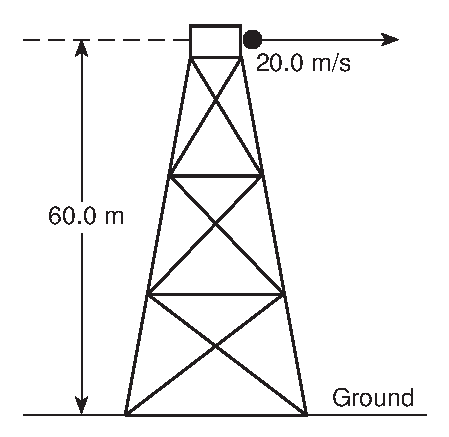
\includegraphics[keepaspectratio,scale=0.95]{Jan2002-Q56}
    \end{center}
    What is the initial vertical velocity of the ball?
    \begin{multicols}{2}
    \begin{choices}
      \correctchoice{\SI{0}{\meter\per\second}}
        \wrongchoice{\SI{9.81}{\meter\per\second}}
        \wrongchoice{\SI{20.0}{\meter\per\second}}
        \wrongchoice{\SI{60.0}{\meter\per\second}}
    \end{choices}
    \end{multicols}
\end{question}
}

\element{nysed}{
\begin{question}{Jan2002-Q57}
    A ball is thrown horizontally with an initial velocity of \SI{20.0}{\meter\per\second} from the top of a tower \SI{60.0}{\meter} high.
    \begin{center}
        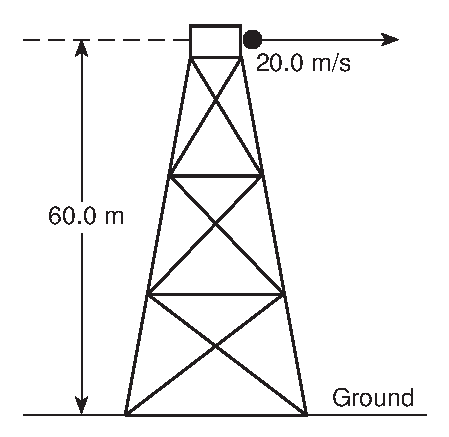
\includegraphics[keepaspectratio,scale=0.95]{Jan2002-Q56}
    \end{center}
    What is the approximate total time required for the ball to reach the ground?
    [Neglect air resistance]
    \begin{multicols}{2}
    \begin{choices}
        \wrongchoice{\SI{12.2}{\second}}
        \wrongchoice{\SI{2.04}{\second}}
        \wrongchoice{\SI{3.00}{\second}}
      \correctchoice{\SI{3.50}{\second}}
    \end{choices}
    \end{multicols}
\end{question}
}

\element{nysed}{
\begin{question}{Jan2002-Q58}
    A ball is thrown horizontally with an initial velocity of \SI{20.0}{\meter\per\second} from the top of a tower \SI{60.0}{\meter} high.
    \begin{center}
        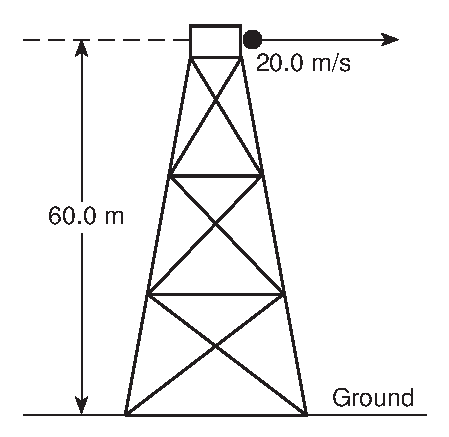
\includegraphics[keepaspectratio,scale=0.95]{Jan2002-Q56}
    \end{center}
    What is the horizontal velocity of the ball just before it reaches the ground?
    [Neglect air resistance.]
    \begin{multicols}{2}
    \begin{choices}
        \wrongchoice{\SI{9.81}{\meter\per\second}}
      \correctchoice{\SI{20.0}{\meter\per\second}}
        \wrongchoice{\SI{34.3}{\meter\per\second}}
        \wrongchoice{\SI{68.6}{\meter\per\second}}
    \end{choices}
    \end{multicols}
\end{question}
}

\element{nysed}{
\begin{question}{Jan2002-Q62}
    A golf ball leaves a golf club with an initial velocity of \SI{40}{\meter\per\second} at an angle of \ang{40} with respect to the horizontal.
    \begin{center}
        \includegraphics[keepaspectratio,scale=0.90]{Jan2002-Q62}
    \end{center}
    What is the vertical component of the golf ball's initial velocity?
    \begin{multicols}{2}
    \begin{choices}
      \correctchoice{\SI{25.7}{\meter\per\second}}
        \wrongchoice{\SI{30.6}{\meter\per\second}}
        \wrongchoice{\SI{40.0}{\meter\per\second}}
        \wrongchoice{\SI{61.3}{\meter\per\second}}
    \end{choices}
    \end{multicols}
\end{question}
}

\element{nysed}{
\begin{question}{Jan2002-Q63}
    A golf ball leaves a golf club with an initial velocity of \SI{40}{\meter\per\second} at an angle of \ang{40} with respect to the horizontal.
    \begin{center}
        \includegraphics[keepaspectratio,scale=0.90]{Jan2002-Q62}
    \end{center}
    What is the total horizontal distance traveled by the golf ball during the first \SI{2.5}{\second} of its flight?
    \begin{multicols}{2}
    \begin{choices}
        \wrongchoice{\SI{100}{\meter}}
      \correctchoice{\SI{76.6}{\meter}}
        \wrongchoice{\SI{64.3}{\meter}}
        \wrongchoice{\SI{40.0}{\meter}}
    \end{choices}
    \end{multicols}
\end{question}
}


%% Section June2001
%%--------------------
\element{nysed}{
\begin{question}{June2001-Q58}
    A red ball and a green ball are simultaneously thrown horizontally from the same height.
    The red ball has an initial speed of \SI{40}{\meter\per\second} and the green ball has an initial speed of \SI{20}{\meter\per\second}.
    Compared to the time it takes the red ball to reach the ground,
        the time it takes the green ball to reach the ground will be:
    \begin{choices}
      \correctchoice{the same}
        \wrongchoice{half as much}
        \wrongchoice{twice as much}
        \wrongchoice{four times as much}
    \end{choices}
\end{question}
}

\element{nysed}{
\begin{question}{June2001-Q59}
    A baseball player throws a ball horizontally.
    Which statement best describes the ball's motion after it is thrown?
    [Neglect the effect of friction.]
    \begin{choices}
        \wrongchoice{Its vertical speed remains the same, and its horizontal speed increases.}
        \wrongchoice{Its vertical speed remains the same, and its horizontal speed remains the same.}
        \wrongchoice{Its vertical speed increases, and its horizontal speed increases.}
      \correctchoice{Its vertical speed increases, and its horizontal speed remains the same.}
    \end{choices}
\end{question}
}


%% Section Jan2001
%%--------------------
\element{nysed}{
\begin{question}{Jan2001-Q58}
    A red ball and a green ball are simultaneously thrown horizontally from the same height.
    the red ball has an initial speed of \SI{40}{\meter\per\second} and the green ball has an initial speed of \SI{20}{\meter\per\second}.
    Compared to the the time it takes the red ball to reach the ground,
        the time it takes the green ball to reach the ground will be:
    \begin{choices}
      \correctchoice{the same}
        \wrongchoice{twice as much}
        \wrongchoice{half as much}
        \wrongchoice{four times as much}
    \end{choices}
\end{question}
}

\element{nysed}{
\begin{question}{Jan2001-Q62}
    The path of a projectile fired at a \ang{30} to the horizontal is best described as:
    \begin{multicols}{2}
    \begin{choices}
      \correctchoice{parabolic}
        \wrongchoice{linear}
        \wrongchoice{circular}
        \wrongchoice{hyperbolic}
    \end{choices}
    \end{multicols}
\end{question}
}


%% Section June2000
%%--------------------
\element{nysed}{
\begin{question}{June2000-Q56}
    A machine launches a tennis ball at an angle of \ang{45} with the horizontal, as shown.
    The ball has an initial vertical velocity of \SI{9.0}{\meter\per\second} and an initial horizontal velocity of \SI{9.0}{\meter\per\second}.
    The ball reaches its maximum height \SI{0.92}{\second} after its launch.
    [Neglect air resistance and assume the ball lands at the same height above the ground from which it was launched.]
    \begin{center}
        \includegraphics[keepaspectratio,width=\columnwidth]{June2000-Q56}
    \end{center}
    The speed of the tennis ball as it leaves the launcher is approximately:
    \begin{multicols}{2}
    \begin{choices}
        \wrongchoice{\SI{4.5}{\meter\per\second}}
      \correctchoice{\SI{13}{\meter\per\second}}
        \wrongchoice{\SI{8.3}{\meter\per\second}}
        \wrongchoice{\SI{18}{\meter\per\second}}
    \end{choices}
    \end{multicols}
\end{question}
}

\element{nysed}{
\begin{question}{June2000-Q57}
    A machine launches a tennis ball at an angle of \ang{45} with the horizontal, as shown.
    The ball has an initial vertical velocity of \SI{9.0}{\meter\per\second} and an initial horizontal velocity of \SI{9.0}{\meter\per\second}.
    The ball reaches its maximum height \SI{0.92}{\second} after its launch.
    [Neglect air resistance and assume the ball lands at the same height above the ground from which it was launched.]
    \begin{center}
        \includegraphics[keepaspectratio,width=\columnwidth]{June2000-Q56}
    \end{center}
    The total horizontal distance traveled by the tennis ball during the entire time it is in the air is approximately:
    \begin{multicols}{2}
    \begin{choices}
        \wrongchoice{\SI{23}{\meter}}
        \wrongchoice{\SI{17}{\meter}}
      \correctchoice{\SI{8.3}{\meter}}
        \wrongchoice{\SI{4.1}{\meter}}
    \end{choices}
    \end{multicols}
\end{question}
}

\element{nysed}{
\begin{question}{June2000-Q58}
    A machine launches a tennis ball at an angle of \ang{45} with the horizontal,
        as shown.
    The ball has an initial vertical velocity of \SI{9.0}{\meter\per\second} and an initial horizontal velocity of \SI{9.0}{\meter\per\second}.
    The ball reaches its maximum height \SI{0.92}{\second} after its launch.
    [Neglect air resistance and assume the ball lands at the same height above the ground from which it was launched.]
    \begin{center}
        \includegraphics[keepaspectratio,width=\columnwidth]{June2000-Q56}
    \end{center}
    The speed at which the launcher fires tennis balls is constant,
        but the angle between the launcher and the horizontal can be varied.
    As the angle is decreased from \ang{45} to \ang{30},
        the range of the tennis balls:
    \begin{choices}
      \correctchoice{decreases}
        \wrongchoice{increases}
        \wrongchoice{remains the same}
    \end{choices}
\end{question}
}

\element{nysed}{
\begin{question}{June2000-Q59}
    A \SI{2}{\kilo\gram} block is dropped from the roof of a tall building at the same time a \SI{6}{\kilo\gram} ball is thrown horizontally from the same height.
    Which statement best describes the motion of the block and the motion of the ball? [Neglect air resistance]
    \begin{choices}
        \wrongchoice{The \SI{2}{\kilo\gram} block hits the ground first because it has no horizontal velocity.}
        \wrongchoice{The \SI{6}{\kilo\gram} block hits the ground first because it has more mass.}
        \wrongchoice{The \SI{6}{\kilo\gram} block hits the ground first because it is round.}
      \correctchoice{The block and the ball hit the ground at the same time because they have the same vertical acceleration}
    \end{choices}
\end{question}
}


%% Section June1999
%%--------------------
\element{nysed}{
\begin{question}{June1999-Q58}
    The diagram below shows the muzzle of a cannon located \SI{50}{\meter} above the ground.
    When the cannon is fired, a ball leaves the muzzle with an initial speed of \SI{250}{\meter\per\second}.
    [Neglect air resistance]
    \begin{center}
    \begin{tikzpicture}[yscale=0.75]
        \draw[very thick] (-2,0) -- (0,0) -- (0,-4) -- (3,-4);
        \draw[fill] (0.2,0.0) circle [radius=2pt];
        \draw[thick,->] (0.2,0.0) -- ++ (0:1)
            node[anchor=south] at ++ (0:-0.5) {$v=\SI{250}{\meter\per\second}$};
        \draw[very thick,dashed] (-2,-4) -- (0,-4);
        \node (A) at (-1,-2.0) {\SI{50}{\meter}};
        \draw[very thick,->] (A) -- (-1,0);
        \draw[very thick,->] (A) -- (-1,-4);
    \end{tikzpicture}
    \end{center}
    Which action would most likely increase the time of flight of the ball fired by the cannon?
    \begin{choices}
        \wrongchoice{pointing the muzzle of the cannon toward the ground}
        \wrongchoice{moving the cannon closer to the edge of the cliff}
      \correctchoice{positioning the cannon higher above the ground}
        \wrongchoice{giving the ball a greater initial horizontal velocity}
    \end{choices}
\end{question}
}

\element{nysed}{
\begin{question}{June1999-Q62}
    In the diagram below,
        a stationary observer on the ground watches as a seagull flying horizontally to the right drops a clamshell.
    \begin{center}
        \includegraphics[keepaspectratio,scale=0.66]{June1999-Q62}
    \end{center}
    Which diagram best represents the path of the falling clamshell as seen by the observer?
    [Neglect air resistance]
    \begin{multicols}{2}
    \begin{choices}
        \AMCboxDimensions{down=-0.40cm}
        \wrongchoice{
            \begin{tikzpicture}
                \draw[white] (-0.5,0) rectangle (0.5,-1);
                \draw[thick,->] (0,0) -- (0,-1);
            \end{tikzpicture}
        }
        \wrongchoice{
            \begin{tikzpicture}
                \draw[white] (-0.15,+0.15) rectangle (+0.85,-0.85);
                \draw[thick,->] (0,0) -- (0.707,-0.707);
            \end{tikzpicture}
        }
        \wrongchoice{
            \begin{tikzpicture}
                \draw[white] (-0.25,0) rectangle (0.75,-1);
                \draw[thick,->] (0,0) arc (90:-90:0.50);
            \end{tikzpicture}
        }
        \correctchoice{
            \begin{tikzpicture}
                \draw[white] (0,1) rectangle (1,0);
                \draw[thick,->] (0,1) parabola (1,0);
            \end{tikzpicture}
        }
    \end{choices}
    \end{multicols}
\end{question}
}


%% Section June1998
%%--------------------
\element{nysed}{
\begin{question}{June1998-Q56}
    A student standing on a knoll throws a snowball horizontally \SI{4.5}{\meter} above the level ground towards a smokestack \SI{15}{\meter} away.
    The snowball hits the smokestack \SI{0.65}{\second} after being released. 
    [Neglect air resistance]
    \begin{center}
        \includegraphics[keepaspectratio,width=\linewidth]{June1998-Q56}
    \end{center}
    Approximately how far above the level ground does the snowball hit the smokestack?
    \begin{multicols}{2}
    \begin{choices}
        \wrongchoice{\SI{0.0}{\meter}}
        \wrongchoice{\SI{0.4}{\meter}}
      \correctchoice{\SI{2.4}{\meter}}
        \wrongchoice{\SI{4.5}{\meter}}
    \end{choices}
    \end{multicols}
\end{question}
}

\element{nysed}{
\begin{question}{June1998-Q57}
    A student standing on a knoll throws a snowball horizontally \SI{4.5}{\meter} above the level ground towards a smokestack \SI{15}{\meter} away.
    The snowball hits the smokestack \SI{0.65}{\second} after being released. 
    [Neglect air resistance]
    \begin{center}
        \includegraphics[keepaspectratio,width=0.95\linewidth]{June1998-Q56}
    \end{center}
    At the instant the snowball is released,
        the horizontal component of its velocity is approximately:
    \begin{multicols}{2}
    \begin{choices}
        \wrongchoice{\SI{6.9}{\meter\per\second}}
        \wrongchoice{\SI{9.8}{\meter\per\second}}
        \wrongchoice{\SI{17}{\meter\per\second}}
      \correctchoice{\SI{23}{\meter\per\second}}
    \end{choices}
    \end{multicols}
\end{question}
}

\element{nysed}{
\begin{question}{June1998-Q62}
    The diagram below shows a projectile moving with speed $v$ at the top of its trajectory.
    \begin{center}
    \begin{tikzpicture}
        %% Ground
        \draw[thick] (-3.5,0) -- (3.5,0);
        \node[anchor=north,fill,pattern=north east lines,minimum width=7cm, minimum height=0.05cm] at (0,0) {};
        \node[anchor=north] at (0,-1em) {Ground};
        %% Path: y = 2/9 x^2, y' = 4/9 x, dy/dx (2) = 12/9, atan(12/9) = 53
        \draw[thick,dashed] (-3,0) parabola bend (0,2) (3,0);
        \draw[thick,->] (-3,0) -- ++(53:1);
        %% Projectile
        \draw[fill] (0,2) circle (3pt) node[anchor=north,yshift=-3pt,font=\small] {Projectile};
        \draw[thick,->] (-0.5,2.4) -- (0.5,2.4) node[pos=0.5,anchor=south] {$v$};
    \end{tikzpicture}
    \end{center}
    Which vector best represents the acceleration of the projectile in the position shown?
    \begin{multicols}{4}
    \begin{choices}
        \AMCboxDimensions{down=-0.2cm}
        \correctchoice{
            \begin{tikzpicture}[scale=0.4]
                \draw[dashed,white!90!black] (0,0) rectangle (2,2);
                \draw[very thick,->] (1,2) -- (1,0);
            \end{tikzpicture}
        }
        \wrongchoice{
            \begin{tikzpicture}[scale=0.4]
                \draw[dashed,white!90!black] (0,0) rectangle (2,2);
                \draw[very thick,->] (2,1) -- (0,1);
            \end{tikzpicture}
        }
        \wrongchoice{
            \begin{tikzpicture}[scale=0.4]
                \draw[dashed,white!90!black] (0,0) rectangle (2,2);
                \draw[very thick,->] (1,0) -- (1,2);
            \end{tikzpicture}
        }
        \wrongchoice{
            \begin{tikzpicture}[scale=0.4]
                \draw[dashed,white!90!black] (0,0) rectangle (2,2);
                \draw[very thick,->] (1,2) -- (1,0);
            \end{tikzpicture}
        }
    \end{choices}
    \end{multicols}
\end{question}
}


%% Section June1997
%%--------------------
\element{nysed}{
\begin{question}{June1997-Q62}
    Projectiles are fired from different angles with the same speed of \SI{14}{\meter\per\second}.
    The graph below shows the range of the projectiles as a function of the original angle of inclination to the ground, neglecting air resistance.
    \begin{center}
    \begin{tikzpicture}
        \begin{axis}[
            axis y line=left, 
            axis x line=bottom, 
            axis line style={->},
            xlabel={Angle},
            x unit=\si{\degree},
            xtick={0,10,20,30,40,50,60,70,80,90},
            ylabel={Range},
            y unit=\si{\meter},
            ytick={0,5,10,15,20},
            grid=major,
            xmin=0,xmax=90,
            ymin=0,ymax=21,
            width=0.8\columnwidth,
            height=0.5\columnwidth,
        ]
        \addplot[line width=1pt,domain=0:90]{20*sin(2*x)};
        \end{axis}
    \end{tikzpicture}
    \end{center}
    The graph shows that the range of the projectile is:
    \begin{choices}
        \wrongchoice{the same for all angles.}
        \wrongchoice{the same for angles of \ang{20} and \ang{80}.}
      \correctchoice{greatest for an angle of \ang{45}.}
        \wrongchoice{greatest for an angle of \ang{90}.}
    \end{choices}
\end{question}
}

\element{nysed}{
\begin{question}{June1997-Q64}
    Four different balls are thrown horizontally off the top of four cliffs.
    In which diagram does the ball have the shortest time of flight?
    \begin{multicols}{2}
    \begin{choices}
        \AMCboxDimensions{down=-1cm}
        \correctchoice{
            \begin{tikzpicture}[font=\footnotesize]
                \draw[dashed,white!90!black] (-1.5,-1.2em) rectangle (1.5,4.3);
                %% Cliff
                \draw[thick] (-1,1) -- (0,1) -- (0,0) -- (1,0);
                \node[anchor=south,rotate=270] at (0,0.5) {Cliff};
                \node[anchor=north,rotate=0.0] at (0.5,0) {Ground};
                %% Height
                \draw[<->] (-0.9,1) -- (-0.9,0) node[pos=0.5,anchor=center,fill=white] {\SI{125}{\meter}};
                %% Mass
                \draw[fill] (0,1.33) circle (1.5pt) node[anchor=east] {\SI{1.0}{\kilo\gram}};
                %% velocity
                \draw[thick,->] (0,1.33) -- ++ (0:1) node[pos=0.5,anchor=south] {\SI{50}{\meter\per\second}};
            \end{tikzpicture}
        }
        \wrongchoice{
            \begin{tikzpicture}[font=\footnotesize]
                \draw[dashed,white!90!black] (-1.5,-1.2em) rectangle (1.5,4.3);
                %% Cliff
                \draw[thick] (-1,2) -- (0,2) -- (0,0) -- (1,0);
                \node[anchor=south,rotate=270] at (0,1.0) {Cliff};
                \node[anchor=north,rotate=0.0] at (0.5,0) {Ground};
                %% Height
                \draw[<->] (-0.9,2) -- (-0.9,0) node[pos=0.5,anchor=center,fill=white] {\SI{250}{\meter}};
                %% Mass
                \draw[fill] (0,2.33) circle (1.5pt) node[anchor=east] {\SI{0.5}{\kilo\gram}};
                %% velocity
                \draw[thick,->] (0,2.33) -- ++ (0:1) node[pos=0.5,anchor=south] {\SI{40}{\meter\per\second}};
            \end{tikzpicture}
        }
        \wrongchoice{
            \begin{tikzpicture}[font=\footnotesize]
                \draw[dashed,white!90!black] (-1.5,-1.2em) rectangle (1.5,4.3);
                %% Cliff
                \draw[thick] (-1,3) -- (0,3) -- (0,0) -- (1,0);
                \node[anchor=south,rotate=270] at (0,1.5) {Cliff};
                \node[anchor=north,rotate=0.0] at (0.5,0) {Ground};
                %% Height
                \draw[<->] (-0.9,3) -- (-0.9,0) node[pos=0.5,anchor=center,fill=white] {\SI{375}{\meter}};
                %% Mass
                \draw[fill] (0,3.33) circle (1.5pt) node[anchor=east] {\SI{0.25}{\kilo\gram}};
                %% velocity
                \draw[thick,->] (0,3.33) -- ++ (0:1) node[pos=0.5,anchor=south] {\SI{35}{\meter\per\second}};
            \end{tikzpicture}
        }
        \wrongchoice{
            \begin{tikzpicture}[font=\footnotesize]
                \draw[dashed,white!90!black] (-1.5,-1.2em) rectangle (1.5,4.3);
                %% Cliff
                \draw[thick] (-1,3.6) -- (0,3.6) -- (0,0) -- (1,0);
                \node[anchor=south,rotate=270] at (0,1.5) {Cliff};
                \node[anchor=north,rotate=0.0] at (0.5,0) {Ground};
                %% Height
                \draw[<->] (-0.9,3.6) -- (-0.9,0) node[pos=0.5,anchor=center,fill=white] {\SI{450}{\meter}};
                %% Mass
                \draw[fill] (0,3.9) circle (1.5pt) node[anchor=east] {\SI{0.1}{\kilo\gram}};
                %% velocity
                \draw[thick,->] (0,3.9) -- ++ (0:1) node[pos=0.5,anchor=south] {\SI{35}{\meter\per\second}};
            \end{tikzpicture}
        }
    \end{choices}
    \end{multicols}
\end{question}
}


%% Section June1996
%%--------------------
\newcommand{\JuneNineteenNinetySixQFiftySix}{
\begin{tikzpicture}
    %% NOTE: useful reference
    %% \frac{h}{R} = \frac{\tan\theta}{4}
    \draw[thick] (-3.5,0) -- (3.5,0);
    \draw[thick,dashed] (-3,0) parabola bend (0,1.05) (3,0);
    \draw[very thick,->] (-3,0) -- ++ (35:2.0cm) node[pos=1.0,anchor=south] {$v_i$};
    \draw[thick,<->] (-2,0) arc (0:35:1cm) node[pos=0.5,anchor=west] {\ang{35}};
\end{tikzpicture}
}

\element{nysed}{
\begin{question}{June1996-Q56}
    A cannon elevated at an angle of \ang{35} to the horizontal fires a cannonball,
        which travels the path shown in the diagram below.
    [Neglect air resistance and assume the ball lands at the same height above the ground from which it was launched.]
    \begin{center}
        \JuneNineteenNinetySixQFiftySix
    \end{center}
    If the ball lands \SI{7.0e2}{\meter} from the cannon \SI{10}{\second} after it was fired,
        what is the horizontal component of its initial velocity?
    \begin{multicols}{2}
    \begin{choices}
      \correctchoice{\SI{70}{\meter\per\second}}
        \wrongchoice{\SI{49}{\meter\per\second}}
        \wrongchoice{\SI{35}{\meter\per\second}}
        \wrongchoice{\SI{7.0}{\meter\per\second}}
    \end{choices}
    \end{multicols}
\end{question}
}

\element{nysed}{
\begin{question}{June1996-Q57}
    A cannon elevated at an angle of \ang{35} to the horizontal fires a cannonball,
        which travels the path shown in the diagram below.
    [Neglect air resistance and assume the ball lands at the same height above the ground from which it was launched.]
    \begin{center}
        \JuneNineteenNinetySixQFiftySix
    \end{center}
    If the ball's time of flight is \SI{10}{\second},
        what is the vertical component of its initial velocity?
    \begin{multicols}{2}
    \begin{choices}
        \wrongchoice{\SI{9.8}{\meter\per\second}}
      \correctchoice{\SI{49}{\meter\per\second}}
        \wrongchoice{\SI{70}{\meter\per\second}}
        \wrongchoice{\SI{98}{\meter\per\second}}
    \end{choices}
    \end{multicols}
\end{question}
}

\element{nysed}{
\begin{question}{June1996-Q58}
    A cannon elevated at an angle of \ang{35} to the horizontal fires a cannonball,
        which travels the path shown in the diagram below.
    [Neglect air resistance and assume the ball lands at the same height above the ground from which it was launched.]
    \begin{center}
        \JuneNineteenNinetySixQFiftySix
    \end{center}
    If the angle of elevation of the cannon is decreased from \ang{35} to \ang{30},
        the vertical component of the ball's initial velocity will:
    \begin{choices}
        \wrongchoice{decrease and its horizontal will decrease.}
      \correctchoice{decrease and its horizontal will increase.}
        \wrongchoice{increase and its horizontal will decrease.}
        \wrongchoice{increase and its horizontal will increase.}
    \end{choices}
\end{question}
}

\element{nysed}{
\begin{question}{June1996-Q65}
    A ball is projected horizontally to the right from a height of \SI{50}{\meter},
        as shown in the diagram below.
    \begin{center}
    \begin{tikzpicture}[yscale=0.75]
        \draw[very thick] (-2,0) -- (0,0) -- (0,-4) -- (3,-4);
        \draw[fill] (0.2,0.0) circle [radius=2pt];
        \draw[thick,->] (0.2,0.0) -- ++ (0:1)
            node[anchor=south] at ++ (0:-0.5) {$v$};
        \draw[very thick,dashed] (-2,-4) -- (0,-4);
        \node (A) at (-1,-2.0) {\SI{50}{\meter}};
        \draw[very thick,->] (A) -- (-1,0);
        \draw[very thick,->] (A) -- (-1,-4);
    \end{tikzpicture}
    \end{center}
    Which diagram best represents the position of the ball at \SI{1.0}{\second} intervals?
    [Neglect air resistance.]
    \begin{multicols}{2}
    \begin{choices}
        \AMCboxDimensions{down=-1.5em}
        \correctchoice{
            \begin{tikzpicture}[yscale=0.75]
                \draw[very thick] (0,0) -- (0,-4) -- (2,-4);
                \draw[domain=0:3.8,samples=4,mark=*,only marks] plot ({0.2+0.4*\x}, {-0.25*\x*\x});
            \end{tikzpicture}
        }
        \wrongchoice{
            \begin{tikzpicture}[yscale=0.75]
                \draw[very thick] (0,0) -- (0,-4) -- (2,-4);
                \draw[domain=0:3.8,samples=4,mark=*,only marks] plot (0.2, {-0.25*\x*\x});
            \end{tikzpicture}
        }
        \wrongchoice{
            \begin{tikzpicture}[yscale=0.75]
                \draw[very thick] (0,0) -- (0,-4) -- (2,-4);
                \draw[domain=0:3.8,samples=4,mark=*,only marks] plot ({0.2+0.10*\x*\x}, {-0.25*\x*\x});
            \end{tikzpicture}
        }
        \wrongchoice{
            \begin{tikzpicture}[yscale=0.75]
                \draw[very thick] (0,0) -- (0,-4) -- (2,-4);
                \draw[domain=0:3.8,samples=4,mark=*,only marks] plot ({0.2+0.3*\x}, {-1.0*\x});
            \end{tikzpicture}
        }
    \end{choices}
    \end{multicols}
\end{question}
}

\endinput



%\input{./qbank/nysed/NYSED-circular.tex}
%\input{./qbank/nysed/NYSED-internalEnergy.tex}
%\input{./qbank/nysed/NYSED-nuclearEnergy.tex}
%\input{./qbank/nysed/NYSED-modern.tex}
%
%% DC Circuit and Kirchoff's Laws Questions for the
%% NYSED Physics Regents Examination
%%--------------------------------------------------

%% this section contains 85 problems


%% Section June2016
%%--------------------
\element{nysed}{
\begin{question}{June2016-Q33}
    Which circuit has the largest equivalent resistance?
    \begin{choices}
        \AMCboxDimensions{down=-0.75cm}
        \ctikzset{bipoles/length=0.75cm}
        \wrongchoice{
            \begin{circuitikz}
                \draw (0,0) to [battery,l=\SI{12}{\volt}] (0,2)
                            to [R,l_=\SI{2}{\ohm}] (4,2)
                            to [R,l=\SI{2}{\ohm}] (4,0)
                            to [R,l_=\SI{4}{\ohm}] (0,0);
            \end{circuitikz}
        }
        \wrongchoice{
            \begin{circuitikz}
                \draw (0,0) to [battery,l=\SI{12}{\volt}] (0,2) to (1.3,2)
                            to [R,l=\SI{2}{\ohm}] (1.3,0) to (0,0);
                \draw (1.3,2) to (2.6,2)
                            to [R,l=\SI{2}{\ohm}] (2.6,0) to (1.3,0);
                \draw (2.6,2) to (4,2)
                            to [R,l=\SI{4}{\ohm}] (4,0) to (2.6,0);
            \end{circuitikz}
        }
        %% ANS is 3
        \correctchoice{
            \begin{circuitikz}
                \draw (0,0) to [battery,l=\SI{12}{\volt}] (0,2)
                            to [R,l_=\SI{2}{\ohm}] (4,2)
                            to [R,l=\SI{2}{\ohm}] (4,0)
                            to [R,l_=\SI{6}{\ohm}] (0,0);
            \end{circuitikz}
        }
        \wrongchoice{
            \begin{circuitikz}
                \draw (0,0) to [battery,l=\SI{12}{\volt}] (0,2) to (1.3,2)
                            to [R,l=\SI{2}{\ohm}] (1.3,0) to (0,0);
                \draw (1.3,2) to (2.6,2)
                            to [R,l=\SI{2}{\ohm}] (2.6,0) to (1.3,0);
                \draw (2.6,2) to (4,2)
                            to [R,l=\SI{6}{\ohm}] (4,0) to (2.6,0);
            \end{circuitikz}
        }
    \end{choices}
\end{question}
}


%% Section June2015
%%--------------------
\element{nysed}{
\begin{question}{June2015-Q19}
    If several resistors are connected in series in an electric circuit,
        the potential difference across each resistor:
    \begin{choices}
      \correctchoice{varies directly with its resistance.}
        \wrongchoice{varies inversely with its resistance.}
        \wrongchoice{varies inversely with the square of its resistance.}
        \wrongchoice{is independent of its resistance.}
    \end{choices}
\end{question}
}


%% Section June2014
%%--------------------


%% Section June2013
%%--------------------
\element{nysed}{
\begin{question}{June2013-Q31}
    The diagram below shows currents in a segment of an electric circuit.
    \begin{center}
    \ctikzset{bipoles/length=0.75cm}
    \begin{circuitikz}[scale=0.8]
        %% NOTE: this is a good reference
        \draw[thick] (-3,0) to [short,i^>=\SI{5}{\ampere}] (0,0)
                            to [short,i^>=\SI{3}{\ampere}] (3,0);
        \draw[thick] (0,2)  to [short,i^>=\SI{7}{\ampere}] (0,0)
                            to [ammeter] (0,-2);
    \end{circuitikz}
    \end{center}
    What is the reading of the ammeter?
    \begin{multicols}{2}
    \begin{choices}
        \wrongchoice{\SI{1}{\ampere}}
        \wrongchoice{\SI{5}{\ampere}}
      \correctchoice{\SI{9}{\ampere}}
        \wrongchoice{\SI{15}{\ampere}}
    \end{choices}
    \end{multicols}
\end{question}
}


%% Section June2012
%%--------------------
\element{nysed}{
\begin{question}{June2012-Q25}
    A \SI{3.0}{\ohm} resistor and a \SI{6.0}{\ohm} resistor are connected in parallel across a \SI{9}{\volt} battery.
    Which statement best compares the potential difference across each resistor?
    \begin{choices}
      \correctchoice{The potential difference across the \SI{6.0}{\ohm} resistor is the same as the potential difference across the \SI{3.0}{\ohm} resistor}
        \wrongchoice{The potential difference across the \SI{6.0}{\ohm} resistor is twice as great as the potential difference across the \SI{3.0}{\ohm} resistor}
        \wrongchoice{The potential difference across the \SI{6.0}{\ohm} resistor is half as great as the potential difference across the \SI{3.0}{\ohm} resistor}
        \wrongchoice{The potential difference across the \SI{6.0}{\ohm} resistor is four times as great as the potential difference across the \SI{3.0}{\ohm} resistor}
    \end{choices}
\end{question}
}



%% Section June2011
%%--------------------
\element{nysed}{
\begin{question}{June2011-Q22}
    Circuit $A$ has four \SI{3.0}{\ohm} resistors connected in series with a \SI{24}{\volt} battery,
        and circuit $B$ has two \SI{3.0}{\ohm} resistors connected in series with a \SI{24}{\volt} battery.
    Compared to the total potential drop across circuit $A$,
        the total potential drop across circuit $B$ is:
    \begin{choices}
        \wrongchoice{one-half as great}
        \wrongchoice{twice as great}
      \correctchoice{the same}
        \wrongchoice{four times as great}
    \end{choices}
\end{question}
}

\element{nysed}{
\begin{question}{June2011-Q44}
    The diagram below represents a circuit consisting of two resistors connected to a source of potential difference.
    \begin{center}
    \ctikzset{bipoles/length=0.75cm}
    \begin{circuitikz}[xscale=1.25]
        \draw (0,0) to [battery,l=$\SI{120}{\volt}$] (0,2)
                    to [R,l=$\SI{10}{\ohm}$] (2,2)
                    to [R,l=$\SI{20}{\ohm}$] (2,0)
                    to (0,0);
    \end{circuitikz}
    \end{center}
    What is the current through the \SI{20}{\ohm} resistor?
    \begin{multicols}{2}
    \begin{choices}
        \wrongchoice{\SI{0.25}{\ampere}}
        \wrongchoice{\SI{6.0}{\ampere}}
        \wrongchoice{\SI{12}{\ampere}}
      \correctchoice{\SI{4.0}{\ampere}}
    \end{choices}
    \end{multicols}
\end{question}
}


%% Section June2010
%%--------------------
\element{nysed}{
\begin{question}{June2010-Q23}
    Which circuit has the \emph{smallest} equivalent resistance?
    \begin{choices}
        \AMCboxDimensions{down=-0.6cm}
        \wrongchoice{
            \ctikzset{bipoles/length=0.75cm}
            \begin{circuitikz}[xscale=1.33]
                \draw[white] (-0.3cm,-0.3cm) rectangle (4.3cm,1.3cm);
                %% Parallel Two
                \draw (0,0) to [battery] (0,1)
                            to (4,1)
                            to [R,l=\SI{2}{\ohm}] (4,0)
                            to (0,0);
                \draw (2,1) to [R,l=\SI{2}{\ohm}] (2,0);
            \end{circuitikz}
        }
        \wrongchoice{
            \ctikzset{bipoles/length=0.75cm}
            \begin{circuitikz}[xscale=1.33]
                \draw[white] (-0.3cm,-0.3cm) rectangle (4.3cm,1.3cm);
                %% Series Two
                \draw (0,0) to [battery] (0,1)
                            to [R,l_=\SI{2}{\ohm}] (2,1) to (4,1) to (4,0)
                            to [R,l_=\SI{2}{\ohm}] (2,0) to (0,0);
            \end{circuitikz}
        }
        \correctchoice{
            \ctikzset{bipoles/length=0.75cm}
            \begin{circuitikz}[xscale=1.33]
                %% Parallel Four
                \draw[white] (-0.3cm,-0.3cm) rectangle (4.3cm,1.3cm);
                \draw (0,0) to [battery] (0,1)
                            to (4,1)
                            to [R,l=\SI{2}{\ohm}] (4,0)
                            to (0,0);
                \draw (1,1) to [R,l=\SI{2}{\ohm}] (1,0);
                \draw (2,1) to [R,l=\SI{2}{\ohm}] (2,0);
                \draw (3,1) to [R,l=\SI{2}{\ohm}] (3,0);
            \end{circuitikz}
        }
        \wrongchoice{
            \ctikzset{bipoles/length=0.75cm}
            \begin{circuitikz}[xscale=1.33]
                \draw[white] (-0.3cm,-0.3cm) rectangle (4.3cm,1.3cm);
                %% Series Four
                \draw (0,0) to [battery] (0,1)
                            to [R,l_=\SI{2}{\ohm}] (1,1) to (2,1)
                            to [R,l_=\SI{2}{\ohm}] (3,1) to (4,1) to (4,0)
                            to [R,l_=\SI{2}{\ohm}] (3,0) to (2,0)
                            to [R,l_=\SI{2}{\ohm}] (1,0) to (0,0);
            \end{circuitikz}
        }
    \end{choices}
\end{question}
}

\element{nysed}{
\begin{question}{June2010-Q45}
    The circuit diagram below represents four resistors connected to a \SI{12}{\volt} source.
    \begin{center}
    \ctikzset{bipoles/length=0.75cm}
    \begin{circuitikz}[scale=1.0]
        \draw (0,0) to [battery,l=$\SI{12}{\volt}$] (0,2)
                    to [R,l=$\SI{4.0}{\ohm}$] (2,2)
                    to [R,l=$\SI{6.0}{\ohm}$] (4,2)
                    to [R,l=$\SI{8.0}{\ohm}$] (4,0)
                    to [R,l_=$\SI{6.0}{\ohm}$] (0,0);
    \end{circuitikz}
    \end{center}
    What is the total current in the circuit?
    \begin{multicols}{2}
    \begin{choices}
      \correctchoice{\SI{0.50}{\ampere}}
        \wrongchoice{\SI{2.0}{\ampere}}
        \wrongchoice{\SI{8.6}{\ampere}}
        \wrongchoice{\SI{24}{\ampere}}
    \end{choices}
    \end{multicols}
\end{question}
}


%% Section June2009
%%--------------------
\element{nysed}{
\begin{question}{June2009-Q46}
    A \SI{3.0}{\ohm} resistor and a \SI{6.0}{\ohm} resistor are connected in series in an operating electric circuit.
    If the current through the \SI{3.0}{\ohm} resistor is \SI{4.0}{\ampere},
        what is the potential difference across the \SI{6.0}{\ohm} resistor?
    \begin{multicols}{2}
    \begin{choices}
        \wrongchoice{\SI{8.0}{\volt}}
        \wrongchoice{\SI{2.0}{\volt}}
        \wrongchoice{\SI{12}{\volt}}
      \correctchoice{\SI{24}{\volt}}
    \end{choices}
    \end{multicols}
\end{question}
}

\element{nysed}{
\begin{question}{June2009-Q47}
    Which combination of resistors has the \emph{smallest} equivalent resistance?
    \begin{multicols}{2}
    \begin{choices}
        \AMCboxDimensions{down=-0.80cm}
        \ctikzset{bipoles/length=0.75cm}
        \correctchoice{
            \begin{circuitikz}[scale=0.75]
                \draw[draw=white] (-2,-1.5) rectangle (2,1.5);
                \draw node[circ] (A) at (-2,0) {}
                      node[circ] (B) at ( 2,0) {}
                      (A) to (-1,0)
                          to (-1,0.5)
                          to [R,l=\SI{1}{\ohm}] (1,0.5)
                          to (1,0)
                      (B) to (1,0)
                          to (1,-0.5)
                          to [R,l=\SI{1}{\ohm}] (-1,-0.5)
                          to (-1,0);
            \end{circuitikz}
        }
        \wrongchoice{
            \begin{circuitikz}[scale=0.75]
                \draw[draw=white] (-2,-1.5) rectangle (2,1.5);
                \draw node[circ] (A) at (-2,0) {}
                      node[circ] (B) at ( 2,0) {}
                      (A) to (-1,0)
                          to (-1,0.5)
                          to [R,l=\SI{2}{\ohm}] (1,0.5)
                          to (1,0)
                      (B) to (1,0)
                          to (1,-0.5)
                          to [R,l=\SI{2}{\ohm}] (-1,-0.5)
                          to (-1,0);
            \end{circuitikz}
        }
        \wrongchoice{
            \begin{circuitikz}[scale=0.75]
                \draw[draw=white] (-2,-1.5) rectangle (2,1.5);
                \draw node[circ] (A) at (-2,0) {}
                      node[circ] (B) at ( 2,0) {}
                      (A) to [R,l=\SI{2}{\ohm}] (0,0)
                          to [R,l=\SI{2}{\ohm}] (B);
            \end{circuitikz}
        }
        \wrongchoice{
            \begin{circuitikz}[scale=0.75]
                \draw[draw=white] (-2,-1.5) rectangle (2,1.5);
                \draw node[circ] (A) at (-2,0) {}
                      node[circ] (B) at ( 2,0) {}
                      (A) to [R,l=\SI{1}{\ohm}] (0,0)
                          to [R,l=\SI{1}{\ohm}] (B);
            \end{circuitikz}
        }
    \end{choices}
    \end{multicols}
\end{question}
}


%% Section Jan2009
%%--------------------
\element{nysed}{
\begin{question}{Jan2009-Q17}
    Three identical lamps are connected in parallel with each other.
    If the resistance of each lamp is $X$ ohms,
        what is the equivalent resistance of this parallel combination?
    \begin{multicols}{2}
    \begin{choices}
        \wrongchoice{$X\si{\ohm}$}
      \correctchoice{$\dfrac{X}{3}\si{\ohm}$}
        \wrongchoice{$3X\si{\ohm}$}
        \wrongchoice{$\dfrac{3}{X}\si{\ohm}$}
    \end{choices}
    \end{multicols}
\end{question}
}

\element{nysed}{
\begin{question}{Jan2009-Q18}
    A \SI{2.0}{\ohm} resistor and a \SI{4.0}{\ohm} resistor are connected in series with a \SI{12}{\volt} battery.
    If the current through the \SI{2.0}{ohm} resistor is \SI{2.0}{\ampere},
        the current through the \SI{4.0}{\ohm} resistor is:
    \begin{multicols}{2}
    \begin{choices}
        \wrongchoice{\SI{1.0}{\ampere}}
      \correctchoice{\SI{2.0}{\ampere}}
        \wrongchoice{\SI{3.0}{\ampere}}
        \wrongchoice{\SI{4.0}{\ampere}}
    \end{choices}
    \end{multicols}
\end{question}
}

\element{nysed}{
\begin{question}{Jan2009-Q20}
    In which circuit would current flow through resistor $R_1$,
        but \emph{not} through $R_2$ while switch $S$ is open?
    \begin{multicols}{2}
    \begin{choices}
        \AMCboxDimensions{down=-2.5em}
        \ctikzset{bipoles/length=0.75cm}
        \correctchoice{
            \begin{circuitikz}[scale=1.0]
                \draw (0,0) to [battery] (0,2)
                            to (2,2)
                            to [R,l_=$R_2$] (2,0)
                            to [ospst=$S$,mirror] (1,0)
                            to (0,0);
                \draw (1,2) to [R,l_=$R_1$] (1,0);
            \end{circuitikz}
        }
        \wrongchoice{
            \begin{circuitikz}[scale=1.0]
                \draw (0,0) to [battery] (0,2)
                            to [R,l_=$R_1$] (2,2)
                            to [ospst=$S$,mirror] (2,0)
                            to [R,l_=$R_2$] (0,0);
            \end{circuitikz}
        }
        \wrongchoice{
            \begin{circuitikz}[scale=1.0]
                \draw (0,0) to [battery] (0,2)
                            to (2,2)
                            to [R,l_=$R_2$] (2,0)
                            to (1,0)
                            to [ospst=$S$,mirror] (0,0);
                \draw (1,2) to [R,l_=$R_1$] (1,0);
            \end{circuitikz}
        }
        \wrongchoice{
            \begin{circuitikz}[scale=1.0]
                \draw (0,0) to [battery] (0,2)
                            to (2,2)
                            to [R,l_=$R_2$] (2,0)
                            to (0,0);
                \draw (1,2) to [R,l_=$R_1$] (1,1)
                            to [ospst=$S$,mirror] (1,0);
            \end{circuitikz}
        }
    \end{choices}
    \end{multicols}
\end{question}
}

\element{nysed}{
\begin{question}{Jan2009-Q42}
    In the electric circuit diagram below,
        possible locations of an ammeter and a voltmeter are indicated by circles 1, 2, 3, and 4.
    \begin{center}
    \ctikzset{bipoles/length=1.00cm}
    \begin{circuitikz}[font=\small]
        %% jphafner
        \draw (0,0) to [battery] (0,3) to (2,3) to [R] (2,1.5) to (2,0);
        \draw (2,3) to (4,3) to [R] (4,0) to (0,0);
        %% 1,2,3,4
        \node[draw,circle,fill=white,anchor=center] at (1,3) {$1$};
        \node[draw,circle,fill=white,anchor=center] at (2,0.75) {$2$};
        \draw (0,0.5) -- (-1,0.5) -- (-1,2.5) node[pos=0.5,anchor=center,draw,circle,fill=white] {$4$} -- (0,2.5) ;
        \draw (4,0.5) -- (5,0.5) -- (5,2.5) node[pos=0.5,anchor=center,draw,circle,fill=white] {$3$} -- (4,2.5);
    \end{circuitikz}
    \end{center}
    Where should an ammeter be located to correctly measure the total current and where should a voltmeter be located to correctly measure the total voltage?
    \begin{choices}
      \correctchoice{ammeter at 1 and voltmeter at 4}
        \wrongchoice{ammeter at 2 and voltmeter at 3}
        \wrongchoice{ammeter at 3 and voltmeter at 4}
        \wrongchoice{ammeter at 1 and voltmeter at 2}
    \end{choices}
\end{question}
}

\element{nysed}{
\begin{question}{Jan2009-Q44}
    A \SI{150}{\watt} lightbulb is brighter than a \SI{60}{\watt} lightbulb when both are operating at a potential difference of \SI{110}{\volt}.
    Compared to the resistance of and the current drawn by the \SI{150}{\watt} lightbulb,
        the \SI{60}{\watt} lightbulb has:
    \begin{choices}
        \wrongchoice{less resistance and draws more current.}
        \wrongchoice{less resistance and draws less current.}
        \wrongchoice{more resistance and draws more current.}
      \correctchoice{more resistance and draws less current.}
    \end{choices}
\end{question}
}

\element{nysed}{
\begin{question}{Jan2009-Q45}
    What is the minimum equipment needed to determine the power dissipated in a resistor of unknown value?
    \begin{choices}
        \wrongchoice{a voltmeter, only}
        \wrongchoice{an ammeter, only}
      \correctchoice{a voltmeter and an ammeter, only}
        \wrongchoice{a voltmeter, an ammeter, and a stopwatch}
    \end{choices}
\end{question}
}


%% Section June2008
%%--------------------
\element{nysed}{
\begin{question}{June2008-Q20}
    Three resistors, \SI{4}{\ohm}, \SI{6}{\ohm}, and \SI{8}{\ohm},
        are connected in parallel in an electric circuit.
    The equivalent resistance of the circuit is:
    \begin{choices}
      \correctchoice{less than \SI{4}{\ohm}}
        \wrongchoice{between \SI{4}{\ohm} and \SI{8}{\ohm}}
        \wrongchoice{between \SI{10}{\ohm} and \SI{18}{\ohm}}
        \wrongchoice{\SI{18}{\ohm}}
    \end{choices}
\end{question}
}



%% Section Jan2008
%%--------------------
\element{nysed}{
\begin{question}{Jan2008-Q20}
    A circuit consists of a \SI{10.0}{\ohm} resistor,
        a \SI{15.0}{\ohm} resistor, and a \SI{20.0}{\ohm} resistor connected in parallel across a \SI{9.00}{\volt} battery.
    What is the equivalent resistance of this circuit?
    \begin{multicols}{2}
    \begin{choices}
        \wrongchoice{\SI{0.200}{\ohm}}
        \wrongchoice{\SI{1.95}{\ohm}}
      \correctchoice{\SI{4.62}{\ohm}}
        \wrongchoice{\SI{45.0}{\ohm}}
    \end{choices}
    \end{multicols}
\end{question}
}

\element{nysed}{
\begin{question}{Jan2008-Q22}
    In the circuit diagram below, two \SI{4.0}{\ohm} resistors are connected to a \SI{16}{\volt} battery as shown.
    \begin{center}
    \ctikzset{bipoles/length=0.75cm}
    \begin{circuitikz}[xscale=1.25]
        \draw (0,0) to [battery,l=$\SI{16}{\volt}$] (0,2)
                    to [R,l_=$\SI{4.0}{\ohm}$] (2,2)
                    to (2,0)
                    to [R,l_=$\SI{4.0}{\ohm}$] (0,0);
    \end{circuitikz}
    \end{center}
    The rate at which electrical energy is expended in this circuit is:
    \begin{multicols}{2}
    \begin{choices}
        \wrongchoice{\SI{8.0}{\watt}}
        \wrongchoice{\SI{16}{\watt}}
      \correctchoice{\SI{32}{\watt}}
        \wrongchoice{\SI{64}{\watt}}
    \end{choices}
    \end{multicols}
\end{question}
}



%% Section June2007
%%--------------------
\element{nysed}{
\begin{question}{June2007-Q18}
    A \SI{6.0}{\ohm} lamp requires \SI{0.25}{\ampere} of current to operate.
    In which circuit below would the lamp operate correctly when switch $S$ is closed?
    \begin{choices}
        \AMCboxDimensions{down=-0.75cm}
        \ctikzset{bipoles/length=0.75cm}
        \correctchoice{
            \begin{circuitikz}
                \draw[draw=white] (-0.5,0) rectangle (5.0,2);
                \draw (0,0) to [battery,l_=$\SI{1.5}{\volt}$] (0,2)
                            to (4,2)
                            to [ospst,mirror,l=$S$] (4,0)
                            to [R,l_=$\SI{6.0}{\ohm}$] (0,0);
            \end{circuitikz}
        }
        \wrongchoice{
            \begin{circuitikz}
                \draw[draw=white] (-0.5,0) rectangle (5.0,2);
                \draw (0,0) to (0,2)
                            to (2,2)
                            to [ospst,l=$S$] (2,1);
                \draw (0,0) to (2,0)
                            to [battery,l=$\SI{1.5}{\volt}$] (2,1);
                \draw (2,2) to (4,2)
                            to [R,l^=$\SI{6.0}{\ohm}$] (4,0)
                            to (2,0);
            \end{circuitikz}
        }
        \wrongchoice{
            \begin{circuitikz}
                \draw[draw=white] (-0.5,0) rectangle (5.0,2);
                \draw (0,0) to [ospst,mirror,l=$S$] (0,2)
                            to (2,2)
                            to [battery,l=$\SI{1.5}{\volt}$] (2,0)
                            to (0,0);
                \draw (2,2) to (4,2)
                            to [R,l=$\SI{6.0}{\ohm}$] (4,0)
                            to (2,0);
            \end{circuitikz}
        }
        \wrongchoice{
            \begin{circuitikz}
                \draw[draw=white] (-0.5,0) rectangle (5.0,2);
                \draw (0,0) to [battery,l_=$\SI{1.5}{\volt}$] (0,2)
                            to (4,2)
                            to [ospst,l=$S$] (4,0)
                            to (0,0);
                \draw (2,2) to [R,l=$\SI{6.0}{\ohm}$] (2,0);
            \end{circuitikz}
        }
    \end{choices}
\end{question}
}

\element{nysed}{
\begin{question}{June2007-Q19}
    What is the total current in a circuit consisting of six operating \SI{100}{\watt} lamps connected in parallel to a \SI{120}{\volt} source?
    \begin{multicols}{2}
    \begin{choices}
      \correctchoice{\SI{5}{\ampere}}
        \wrongchoice{\SI{600}{\ampere}}
        \wrongchoice{\SI{12000}{\ampere}}
        \wrongchoice{\SI{20}{\ampere}}
    \end{choices}
    \end{multicols}
\end{question}
}



%% Section Jan2007
%%--------------------
\element{nysed}{
\begin{question}{Jan2007-Q17}
    The diagram below represents a simple circuit consisting of a variable resistor, a battery, an ammeter, and a voltmeter.
    \begin{center}
    \ctikzset{bipoles/length=0.75cm}
    \begin{circuitikz}[yscale=-0.80,xscale=1.5]
        \draw (0,0) to [battery] (2,0)
                    to [ammeter](2,2)
                    to [vR,l_=$R_2$] (0,2)
                    to (0,0);
        \draw (0.5,2) to (0.5,3.0)
                    to [voltmeter] (1.5,3.0)
                    to (1.5,2);
    \end{circuitikz}
    \end{center}
    What is the effect of increasing the resistance of the variable resistor from \SI{1000}{\ohm} to \SI{10000}{\ohm}?
    Assume constant temperature.
    \begin{choices}
      \correctchoice{The ammeter reading decreases.}
        \wrongchoice{The ammeter reading increases.}
        \wrongchoice{The voltmeter reading decreases.}
        \wrongchoice{The voltmeter reading increases.}
    \end{choices}
\end{question}
}

\newcommand{\myJuneZeroSevenQfortyOneTikz}{
    \ctikzset{bipoles/length=0.75cm}
    \begin{circuitikz}[xscale=1.40,font=\small]
        \draw (0,0) to [battery,l_=\SI{12}{\volt}] (0,2)
                    to (1,2)
                    to [R=\SI{6.0}{\ohm}](1,1)
                    to [ammeter](1,0)
                    to (0,0);
        \draw (1,2) to (2,2)
                    to [R,l=$\SI{12}{\ohm}$] (2,0)
                    to (1,0);
        \draw (2,2) to (3,2)
                    to [R,l=$\SI{36}{\ohm}$] (3,0)
                    to (2,0);
        \draw (3,2) to (4,2)
                    to [R,l=$\SI{18}{\ohm}$] (4,0)
                    to (3,0);
    \end{circuitikz}
    %\begin{circuitikz}[xscale=0.75,yscale=0.60]
    %    %\draw (0,0) to [battery,l=$\SI{12}{\volt}$] (0,4)
    %    \draw (-1,4) to [battery,l=$\SI{12}{\volt}$] (-1,0);
    %    \draw (-1,4)to (1,4)
    %                to [R,l=$\SI{6.0}{\ohm}$] (1,2)
    %                to [ammeter,l=$A$] (1,0)
    %                to (-1,0);
    %    \draw (1,4) to (3,4)
    %                to [R,l=$\SI{12}{\ohm}$] (3,0)
    %                to (1,0);
    %    \draw (3,4) to (5,4)
    %                to [R,l=$\SI{36}{\ohm}$] (5,0)
    %                to (3,0);
    %    \draw (5,4) to (7,4)
    %                to [R,l=$\SI{18}{\ohm}$] (7,0)
    %                to (5,0);
    %\end{circuitikz}
}

\element{nysed}{
\begin{question}{Jan2007-Q41}
    The diagram below represents an electric circuit consisting of four resistors and a \SI{12}{\volt} battery.
    \begin{center}
        \myJuneZeroSevenQfortyOneTikz
    \end{center}
    What is the current measured by ammeter $A$?
    \begin{multicols}{2}
    \begin{choices}
      \correctchoice{\SI{2.0}{\ampere}}
        \wrongchoice{\SI{72}{\ampere}}
        \wrongchoice{\SI{4.0}{\ampere}}
        \wrongchoice{\SI{0.50}{\ampere}}
    \end{choices}
    \end{multicols}
\end{question}
}

\element{nysed}{
\begin{question}{Jan2007-Q42}
    The diagram below represents an electric circuit consisting of four resistors and a \SI{12}{\volt} battery.
    \begin{center}
        \myJuneZeroSevenQfortyOneTikz
    \end{center}
    What is the equivalent resistance of this circuit?
    \begin{multicols}{2}
    \begin{choices}
      \correctchoice{\SI{3.0}{\ohm}}
        \wrongchoice{\SI{0.33}{\ohm}}
        \wrongchoice{\SI{72}{\ohm}}
        \wrongchoice{\SI{18}{\ohm}}
    \end{choices}
    \end{multicols}
\end{question}
}

\element{nysed}{
\begin{question}{Jan2007-Q43}
    The diagram below represents an electric circuit consisting of four resistors and a \SI{12}{\volt} battery.
    \begin{center}
    \ctikzset{bipoles/length=0.75cm}
    \begin{circuitikz}[xscale=0.75,yscale=0.60]
        %\draw (0,0) to [battery,l=$\SI{12}{\volt}$] (0,4)
        \draw (-1,4) to [battery,l=$\SI{12}{\volt}$] (-1,0);
        \draw (-1,4)to (1,4)
                    to [R,l=$\SI{6.0}{\ohm}$] (1,2)
                    to [ammeter,l=$A$] (1,0)
                    to (-1,0);
        \draw (1,4) to (3,4)
                    to [R,l=$\SI{12}{\ohm}$] (3,0)
                    to (1,0);
        \draw (3,4) to (5,4)
                    to [R,l=$\SI{36}{\ohm}$] (5,0)
                    to (3,0);
        \draw (5,4) to (7,4)
                    to [R,l=$\SI{18}{\ohm}$] (7,0)
                    to (5,0);
    \end{circuitikz}
    \end{center}
    How much power is dissipated in the \SI{36}{\ohm} resistor?
    \begin{multicols}{2}
    \begin{choices}
      \correctchoice{\SI{4.0}{\watt}}
        \wrongchoice{\SI{3.0}{\watt}}
        \wrongchoice{\SI{110}{\watt}}
        \wrongchoice{\SI{48}{\watt}}
    \end{choices}
    \end{multicols}
\end{question}
}


%% Section June2006
%%--------------------
\element{nysed}{
\begin{question}{June2006-Q20}
    In which circuit represented below are meters properly connected to measure the current through resistor $R_1$ and the potential difference across resistor $R_2$?
    \begin{multicols}{2}
    \begin{choices}
        \AMCboxDimensions{down=-1.5cm}
        \ctikzset{bipoles/length=0.75cm}
        \wrongchoice{
            \begin{circuitikz}
                \draw (0,0) to [R,l=$R_1$] (1,0) to [ammeter] (2,0) to [R,l=$R_2$] (3,0)
                            to [voltmeter] (3,3) to [battery] (0,3) to (0,0);
            \end{circuitikz}
        }
        \wrongchoice{
            \begin{circuitikz}
                \draw (0,0) to [R,l=$R_1$] (1.5,0) to [R,l=$R_2$] (3,0)
                            to (3,2) to [battery] (0,2) to (0,0);
                \draw (0.25,0) to (0.25,-1) to [ammeter] (1.25,-1) to (1.25,0);
                \draw (1.75,0) to (1.75,-1) to [voltmeter] (2.75,-1) to (2.75,0);
            \end{circuitikz}
        }
        \wrongchoice{
            \begin{circuitikz}
                \draw (0,0) to [R,l=$R_2$] (1.5,0) to (3,0)
                            to (3,2) to [battery] (0,2) to (0,0);
                \draw (0,1.25) to (1.5,1.25) to [R,l=$R_1$] (3,1.25);
                \draw (1.75,1.25) to (1.75,0.5) to [ammeter] (2.75,0.5) to (2.74,1.25);
                \draw (0.25,0) to (0.25,-1) to [voltmeter] (1.25,-1) to (1.25,0);
            \end{circuitikz}
        }
        \correctchoice{
            \begin{circuitikz}
                \draw (0,0) to [R,l=$R_2$] (3,0)
                            to (3,2) to [battery] (0,2) to (0,0);
                \draw (0,1) to [R,l=$R_1$] (1.5,1) to [ammeter] (3,1);
                \draw (1,0) to (1,-1) to [voltmeter] (2,-1) to (2,0);
            \end{circuitikz}
        }
    \end{choices}
    \end{multicols}
\end{question}
}

\element{nysed}{
\begin{question}{June2006-Q21}
    Two identical resistors connected in series have an equivalent resistance of \SI{4}{\ohm}.
    The same two resistors, when connected in parallel,
        have an equivalent resistance of:
    \begin{multicols}{2}
    \begin{choices}
      \correctchoice{\SI{1}{\ohm}}
        \wrongchoice{\SI{2}{\ohm}}
        \wrongchoice{\SI{8}{\ohm}}
        \wrongchoice{\SI{4}{\ohm}}
    \end{choices}
    \end{multicols}
\end{question}
}

\element{nysed}{
\begin{question}{June2006-Q24}
    As the number of resistors in a parallel circuit is increased,
        what happens to the equivalent resistance of the circuit and total current in the circuit?
    \begin{choices}
      \correctchoice{Equivalent resistance decreases and total current increases.}
        \wrongchoice{Equivalent resistance decreases and total current decreases.}
        \wrongchoice{Both equivalent resistance and total current increases.}
        \wrongchoice{Both equivalent resistance and total current decreases.}
    \end{choices}
\end{question}
}



%% Section Jan2006
%%--------------------
\element{nysed}{
\begin{question}{Jan2006-Q25}
    What must be inserted between points $A$ and $B$ to establish a steady electrical current in the incomplete circuit represented in the diagram below?
    \begin{center}
    \ctikzset{bipoles/length=1.00cm}
    \begin{circuitikz}[scale=1.5]
        \draw node[circ,label=above:{$A$}] at (-.5,1) {};
        \draw node[circ,label=above:{$B$}] at (.5,1) {} ;
        \draw (-.5,1) to (-1,1)
                    to (-1,0)
                    to [R,l=$R$] (1,0)
                    to (1,1)
                    to (0.5,1);
    \end{circuitikz}
    \end{center}
    \begin{choices}
      \correctchoice{source of potential difference}
        \wrongchoice{switch}
        \wrongchoice{voltmeter}
        \wrongchoice{magnetic field source}
    \end{choices}
\end{question}
}

\element{nysed}{
\begin{question}{Jan2006-Q26}
    In a series of circuit containing two lamps,
        the battery supplies a potential difference of \SI{1.5}{\volt}.
    If the current in the circuit is \SI{0.10}{\ampere},
        at what rate does the circuit use energy?
    \begin{multicols}{2}
    \begin{choices}
      \correctchoice{\SI{0.15}{\watt}}
        \wrongchoice{\SI{0.015}{\watt}}
        \wrongchoice{\SI{1.5}{\watt}}
        \wrongchoice{\SI{15}{\watt}}
    \end{choices}
    \end{multicols}
\end{question}
}



%% Section June2005
%%--------------------
\element{nysed}{
\begin{question}{June2005-Q22}
    The diagram below represents part of an electric circuit containing three resistors.
    \begin{center}
    \ctikzset{bipoles/length=0.75cm}
    \begin{circuitikz}[scale=1.25]
        \draw (0,0) to [R,l=$\SI{4}{\ohm}$,*-*] (4,0);
        \draw (1,0) to (1,1)
                    to [R,l=$\SI{3}{\ohm}$] (3,1)
                    to (3,0);
        \draw (1,0) to (1,-1)
                    to [R,l=$\SI{12}{\ohm}$] (3,-1)
                    to (3,0);
    \end{circuitikz}
    \end{center}
    What is the equivalent resistance of this part of the circuit?
    \begin{multicols}{2}
    \begin{choices}
      \correctchoice{\SI{1.5}{\ohm}}
        \wrongchoice{\SI{0.67}{\ohm}}
        \wrongchoice{\SI{6.3}{\ohm}}
        \wrongchoice{\SI{19}{\ohm}}
    \end{choices}
    \end{multicols}
\end{question}
}

\element{nysed}{
\begin{question}{June2005-Q23}
    %In the circuit represented by the diagram below, what is the reading of voltmeter $V$?
    In the circuit diagram below,
        two resistors are connected in series to a \SI{60}{\volt} battery.
    \begin{center}
    \ctikzset{bipoles/length=0.75cm}
    \begin{circuitikz}[scale=1.25]
        \draw (0,0) to [battery,l=$\SI{60}{\volt}$] (0,2)
                    to [R,l_=$\SI{20}{\ohm}$] (2,2)
                    to [R,l=$\SI{10}{\ohm}$] (2,0)
                    to (0,0);
        \draw (0.5,2) to (0.5,2.5)
                    to [voltmeter] (1.5,2.5)
                    to (1.5,2);
    \end{circuitikz}
    \end{center}
    What is the reading of the voltmeter?
    \begin{multicols}{2}
    \begin{choices}
      \correctchoice{\SI{40}{\volt}}
        \wrongchoice{\SI{30}{\volt}}
        \wrongchoice{\SI{20}{\volt}}
        \wrongchoice{\SI{2.0}{\volt}}
    \end{choices}
    \end{multicols}
\end{question}
}


%% Section Jan2005
%%--------------------
\element{nysed}{
\begin{question}{Jan2005-Q29}
    A \SI{9.0}{\volt} battery is connected to a \SI{4.0}{\ohm} resistor and a \SI{5.0}{\ohm} resistor as shown in the diagram below.
    \begin{center}
    \ctikzset{bipoles/length=0.75cm}
    \begin{circuitikz}[scale=1.0]
        \draw (0,0) to [battery,l=$\SI{9}{\volt}$] (0,2)
                    to [R,l=$\SI{4.0}{\ohm}$] (2,2)
                    to [R,l=$\SI{5.0}{\ohm}$] (2,0)
                    to (0,0);
    \end{circuitikz}
    \end{center}
    What is the current in the \SI{5.0}{\ohm} resistor?
    \begin{multicols}{2}
    \begin{choices}
      \correctchoice{\SI{1.0}{\ampere}}
        \wrongchoice{\SI{1.8}{\ampere}}
        \wrongchoice{\SI{2.3}{\ampere}}
        \wrongchoice{\SI{4.0}{\ampere}}
    \end{choices}
    \end{multicols}
\end{question}
}

\element{nysed}{
\begin{question}{Jan2005-Q30}
    A \SI{100}{\ohm} resistor and an unknown resistor are connected in series to a \SI{10.0}{\volt} battery.
    If the potential drop across the \SI{100}{\ohm} resistor is \SI{4.00}{\volt},
        the resistance of the unknown resistor is:
    \begin{multicols}{2}
    \begin{choices}
      \correctchoice{\SI{150}{\ohm}}
        \wrongchoice{\SI{100}{\ohm}}
        \wrongchoice{\SI{200}{\ohm}}
        \wrongchoice{\SI{50.0}{\ohm}}
    \end{choices}
    \end{multicols}
\end{question}
}

\element{nysed}{
\begin{question}{Jan2005-Q42}
    In the circuit diagram shown below,
        ammeter $A_1$ reads \SI{10.}{\ampere}.
    \begin{center}
    \ctikzset{bipoles/length=0.75cm}
    \begin{circuitikz}[scale=1.25]
        \draw (0,0) to [battery,l=$\SI{12}{\volt}$] (0,2)
                    to [ammeter,i=$\SI{10}{\ampere}$,l=$A_1$] (2,2)
                    to [ammeter,l=$A_{2}$](2,1)
                    to [R,l=$\SI{20}{\ohm}$](2,0)
                    to (0,0);
        \draw (2,2) to (4,2)
                    to [ammeter,l=$A_{3}$](4,1)
                    to [R,l=$\SI{30}{\ohm}$] (4,0)
                    to (2,0);
    \end{circuitikz}
    \end{center}
    What is the reading of ammeter $A_2$?
    \begin{multicols}{2}
    \begin{choices}
      \correctchoice{\SI{6.0}{\ampere}}
        \wrongchoice{\SI{10.}{\ampere}}
        \wrongchoice{\SI{20}{\ampere}}
        \wrongchoice{\SI{4.0}{\ampere}}
    \end{choices}
    \end{multicols}
\end{question}
}


%% Section June2004
%%--------------------
\element{nysed}{
\begin{question}{June2004-Q23}
    The diagram below represents an electric circuit consisting of a \SI{12}{\volt} battery, a \SI{3.0}{\ohm} resistor,
        $R_1$, and a variable resistor, $R_2$.
    \begin{center}
    \ctikzset{bipoles/length=1.00cm}
    \begin{circuitikz}
        \draw (0,0) to [battery,l=$\SI{12}{\volt}$] (0,2)
                    to [R=$R_1$] (3,2)
                    to [vR=$R_2$] (3,0)
                    to (0,0);
        \node[anchor=north] at (1.5,1.8) {\SI{3.0}{\ohm}};
    \end{circuitikz}
    \end{center}
    At what value must the variable resistor be set to produce a current of \SI{1.0}{\ampere} through $R_1$?
    \begin{multicols}{2}
    \begin{choices}
      \correctchoice{\SI{9.0}{\ohm}}
        \wrongchoice{\SI{6.0}{\ohm}}
        \wrongchoice{\SI{3.0}{\ohm}}
        \wrongchoice{\SI{12}{\ohm}}
    \end{choices}
    \end{multicols}
\end{question}
}

\element{nysed}{
\begin{question}{June2004-Q42}
    A \SI{20}{\ohm} resistor and a \SI{30}{\ohm} resistor are connected in parallel to a \SI{12}{\volt} battery as shown.
    An ammeter is connected as shown.
    \begin{center}
    \ctikzset{bipoles/length=0.75cm}
    \begin{circuitikz}[scale=1.0]
        \draw (0,0) to [battery,l=$\SI{12}{\volt}$] (0,2)
                    to (2,2)
                    to [ammeter](2,1)
                    to [R,l=$\SI{20}{\ohm}$](2,0)
                    to (0,0);
        \draw (2,2) to (4,2)
                    to [R,l=$\SI{30}{\ohm}$] (4,0)
                    to (2,0);
    \end{circuitikz}
    \end{center}
    What is the equivalent resistance of the circuit?
    \begin{multicols}{2}
    \begin{choices}
      \correctchoice{\SI{12}{\ohm}}
        \wrongchoice{\SI{10}{\ohm}}
        \wrongchoice{\SI{25}{\ohm}}
        \wrongchoice{\SI{50}{\ohm}}
    \end{choices}
    \end{multicols}
\end{question}
}

\element{nysed}{
\begin{question}{June2004-Q43}
    A \SI{20}{\ohm} resistor and a \SI{30}{\ohm} resistor are connected in parallel to a \SI{12}{\volt} battery as shown.
    An ammeter is connected as shown.
    \begin{center}
    \ctikzset{bipoles/length=0.75cm}
    \begin{circuitikz}[scale=1.0]
        \draw (0,0) to [battery,l=$\SI{12}{\volt}$] (0,2)
                    to (2,2)
                    to [ammeter](2,1)
                    to [R,l=$\SI{20}{\ohm}$](2,0)
                    to (0,0);
        \draw (2,2) to (4,2)
                    to [R,l=$\SI{30}{\ohm}$] (4,0)
                    to (2,0);
    \end{circuitikz}
    \end{center}
    What is the current reading of the ammeter?
    \begin{multicols}{2}
    \begin{choices}
      \correctchoice{\SI{0.60}{\ampere}}
        \wrongchoice{\SI{1.0}{\ampere}}
        \wrongchoice{\SI{0.40}{\ampere}}
        \wrongchoice{\SI{0.20}{\ampere}}
    \end{choices}
    \end{multicols}
\end{question}
}

\element{nysed}{
\begin{question}{June2004-Q44}
    A \SI{20}{\ohm} resistor and a \SI{30}{\ohm} resistor are connected in parallel to a \SI{12}{\volt} battery as shown.
    An ammeter is connected as shown.
    \begin{center}
    \ctikzset{bipoles/length=0.75cm}
    \begin{circuitikz}[scale=1.0]
        \draw (0,0) to [battery,l=$\SI{12}{\volt}$] (0,2)
                    to (2,2)
                    to [ammeter](2,1)
                    to [R,l=$\SI{20}{\ohm}$](2,0)
                    to (0,0);
        \draw (2,2) to (4,2)
                    to [R,l=$\SI{30}{\ohm}$] (4,0)
                    to (2,0);
    \end{circuitikz}
    \end{center}
    What is the power of the \SI{30}{\ohm} resistor?
    \begin{multicols}{2}
    \begin{choices}
      \correctchoice{\SI{4.8}{\watt}}
        \wrongchoice{\SI{30}{\watt}}
        \wrongchoice{\SI{12}{\watt}}
        \wrongchoice{\SI{75}{\watt}}
    \end{choices}
    \end{multicols}
\end{question}
}


%% Section Jan2004
%%--------------------
\element{nysed}{
\begin{question}{Jan2004-Q15}
    %In which circuit would ammeter $A$ show the greatest current?
    In which circuit would the ammeter show the greatest current?
    \begin{choices}
        \AMCboxDimensions{down=-0.75cm}
        \ctikzset{bipoles/length=0.75cm}
        \correctchoice{
            \begin{circuitikz}[xscale=1.25]
                \draw (0,0) to [ammeter] (0,1)
                            to [battery,l=$\SI{1.5}{\volt}$] (0,2)
                            to (1,2)
                            to [R,l=$\SI{5}{\ohm}$] (1,0)
                            to (0,0);
                \draw (1,2) to (2,2)
                            to [R,l=$\SI{5}{\ohm}$] (2,0)
                            to (1,0);
                \draw (2,2) to (3,2)
                            to [R,l=$\SI{5}{\ohm}$] (3,0)
                            to (2,0);
            \end{circuitikz}
        }
        \wrongchoice{
            \begin{circuitikz}[xscale=1.25]
                \draw (0,0) to [ammeter] (0,1)
                            to [battery,l=$\SI{1.5}{\volt}$] (0,2)
                            to [R,l=$\SI{5}{\ohm}$] (2,2)
                            to [R,l=$\SI{5}{\ohm}$] (2,0)
                            to (0,0);
            \end{circuitikz}
        }
        \wrongchoice{
            \begin{circuitikz}[xscale=1.25]
                \draw (0,0) to [ammeter] (0,1)
                            to [battery,l=$\SI{1.5}{\volt}$] (0,2)
                            to (1,2)
                            to [R,l=$\SI{5}{\ohm}$] (1,0)
                            to (0,0);
                \draw (1,2) to (2,2)
                            to [R,l=$\SI{5}{\ohm}$] (2,0)
                            to (1,0);
            \end{circuitikz}
        }
        \wrongchoice{
            \begin{circuitikz}[xscale=1.25]
                \draw (0,0) to [ammeter] (0,1)
                            to [battery,l=$\SI{1.5}{\volt}$] (0,2)
                            to (2,2)
                            to [R,l=$\SI{5}{\ohm}$] (2,0)
                            to (0,0);
            \end{circuitikz}
        }
    \end{choices}
\end{question}
}

\element{nysed}{
\begin{question}{Jan2004-Q44}
    The diagram below represents a lamp, a \SI{10}{\volt} battery,
        and a length of nichrome wire connected in series.
    \begin{center}
    \ctikzset{bipoles/length=0.75cm}
    \begin{circuitikz}[scale=1.0]
        \draw (0,0) to [battery,l=$\SI{10}{\volt}$] (0,2)
                    to [R,l={Lamp}] (2,2)
                    to [european resistor,l={Nichrome}] (2,0)
                    to (0,0);
    \end{circuitikz}
    \end{center}
    As the temperature of the nichrome is decreased,
        the brightness of lamp will:
    \begin{choices}
      \correctchoice{increase}
        \wrongchoice{decrease}
        \wrongchoice{remain the same}
    \end{choices}
\end{question}
}

\newcommand{\myJanZeroFourQfortyFiveTikz}{
    \ctikzset{bipoles/length=0.75cm}
    \begin{circuitikz}%[xscale=1.40,font=\small]
        \draw (0,0) to [battery,l_=\SI{24}{\volt}] (0,2)
                    to [ammeter] (2,2)
                    to [R,l=\SI{4.0}{\ohm}] (2,1)
                    to [cspst,l=$S$] (2,0)
                    to (0,0);
        \draw (2,2) to (4,2)
                    to [R,l=$\SI{12}{\ohm}$] (4,0)
                    to (2,0);
    \end{circuitikz}
}

\element{nysed}{
\begin{question}{Jan2004-Q45}
    The diagram below shows two resistors connected in parallel to a \SI{24}{\volt} battery.
    \begin{center}
        \myJanZeroFourQfortyFiveTikz
    \end{center}
    If switch $S$ is open, the reading of ammeter $A$ is:
    %If the switch is open, the ammeter reading is
    \begin{multicols}{2}
    \begin{choices}
      \correctchoice{\SI{2.0}{\ampere}}
        \wrongchoice{\SI{0.50}{\ampere}}
        \wrongchoice{\SI{1.5}{\ampere}}
        \wrongchoice{\SI{6.0}{\ampere}}
    \end{choices}
    \end{multicols}
\end{question}
}

\element{nysed}{
\begin{question}{Jan2004-Q46}
    The diagram below shows two resistors connected in parallel to a \SI{24}{\volt} battery.
    \begin{center}
        \myJanZeroFourQfortyFiveTikz
    \end{center}
    %If the switch is closed, the equivalent resistance of the circuit is
    If switch $S$ is closed, the equivalent resistance of the circuit is:
    \begin{multicols}{2}
    \begin{choices}
      \correctchoice{\SI{3.0}{\ohm}}
        \wrongchoice{\SI{16}{\ohm}}
        \wrongchoice{\SI{8.0}{\ohm}}
        \wrongchoice{\SI{2.0}{\ohm}}
    \end{choices}
    \end{multicols}
\end{question}
}


%% Section June2003
%%--------------------
\element{nysed}{
\begin{question}{June2003-Q24}
    Two identical resistors connected in parallel have an equivalent resistance of \SI{40}{\ohm}.
    What is the resistance of each resistor?
    \begin{multicols}{2}
    \begin{choices}
      \correctchoice{\SI{20}{\ohm}}
        \wrongchoice{\SI{40}{\ohm}}
        \wrongchoice{\SI{80}{\ohm}}
        \wrongchoice{\SI{160}{\ohm}}
    \end{choices}
    \end{multicols}
\end{question}
}

\element{nysed}{
\begin{question}{June2003-Q43}
    %Which circuit diagram correctly shows the connection of ammeter $A$ and voltmeter $V$ to measure the current through and potential differences across resistor $R$?
    Which circuit diagram correctly shows the connection of an ammeter and a voltmeter to measure the current through and potential differences across resistor $R$?
    \begin{choices}
        \AMCboxDimensions{down=-1.0cm}
        \ctikzset{bipoles/length=0.75cm}
        \correctchoice{
            \begin{circuitikz}[scale=1.0]
                \draw[draw=white] (-0.5,0) rectangle (5.0,2);
                \draw (0,0) to [battery] (0,2)
                            to [ammeter,l_=$A$] (2,2)
                            to [R,l=$R$] (2,0)
                            to (0,0);
                \draw (2,2) to (4,2)
                            to [voltmeter,l=$V$] (4,0)
                            to (2,0);
            \end{circuitikz}
        }
        \wrongchoice{
            \begin{circuitikz}[scale=1.0]
                \draw[draw=white] (-0.5,0) rectangle (5.0,2);
                \draw (0,0) to [battery] (0,2)
                            to [ammeter,l_=$A$] (4,2)
                            to [voltmeter,l=$V$] (4,0)
                            to [R,l_=$R$] (0,0);
            \end{circuitikz}
        }
        \wrongchoice{
            \begin{circuitikz}[scale=1.0]
                \draw[draw=white] (-0.5,0) rectangle (5.0,2);
                \draw (0,0) to [battery] (0,2)
                            to (1.33,2)
                            to [R,l=$R$] (1.33,0)
                            to (0,0);
                \draw (1.33,2) to (2.66,2)
                            to [ammeter,l=$A$] (2.66,0)
                            to (1.33,0);
                \draw (2.66,2) to (4,2)
                            to [voltmeter,l=$V$] (4,0)
                            to (2.66,0);
            \end{circuitikz}
        }
        \wrongchoice{
            \begin{circuitikz}[scale=1.0]
                \draw[draw=white] (-0.5,0) rectangle (5.0,2);
                \draw (0,0) to [battery] (0,2)
                            to (2,2)
                            to [R,l=$R$] (2,0)
                            to (0,0);
                \draw (2,2) to [ammeter,l_=$A$] (4,2)
                            to [voltmeter,l=$V$] (4,0)
                            to (2,0);
            \end{circuitikz}
        }
    \end{choices}
\end{question}
}

\element{nysed}{
\begin{question}{June2003-Q44}
    Identical resistors ($R$) are connected across the same \SI{12}{\volt} battery.
    Which circuit uses the greatest power?
    \begin{choices}
        \AMCboxDimensions{down=-0.5em}
        \ctikzset{bipoles/length=0.75cm}
        \correctchoice{
            \begin{circuitikz}[scale=1.0]
                \draw (0,0) to [battery,l=$\SI{12}{\volt}$] (0,1)
                            to (4,1)
                            to [R,l=$R$] (4,0)
                            to (0,0);
                \draw (1,1) to [R,l=$R$] (1,0);
                \draw (2,1) to [R,l=$R$] (2,0);
                \draw (3,1) to [R,l=$R$] (3,0);
            \end{circuitikz}
        }
        \wrongchoice{
            \begin{circuitikz}[scale=1.0]
                \draw (0,0) to [battery,l=$\SI{12}{\volt}$] (0,1)
                            to (4,1)
                            to [R,l=$R$] (4,0)
                            to (0,0);
            \end{circuitikz}
        }
        \wrongchoice{
            \begin{circuitikz}[scale=1.0]
                \draw (0,0) to [battery,l=$\SI{12}{\volt}$] (0,1)
                            to [R,l_=$R$] (2,1)
                            to (4,1)
                            to [R,l=$R$] (4,0)
                            to [R,l_=$R$] (2,0)
                            to (0,0);
            \end{circuitikz}
        }
        \wrongchoice{
            \begin{circuitikz}[scale=1.0]
                \draw (0,0) to [battery,l=$\SI{12}{\volt}$] (0,1)
                            to (4,1)
                            to [R,l=$R$] (4,0)
                            to (0,0);
                \draw (2,1) to [R,l=$R$] (2,0);
            \end{circuitikz}
        }
    \end{choices}
\end{question}
}


%% Section Jan2003
%%--------------------
\element{nysed}{
\begin{question}{Jan2003-Q43}
    The diagram below shows a circuit with two resistors.
    \begin{center}
    \ctikzset{bipoles/length=0.75cm}
    \begin{circuitikz}[scale=1.2]
        \draw (0,0) to [battery,l=\SI{12}{\volt}] (2,0)
                    to [ammeter] (4,0)
                    to (4,2)
                    to [R,l_=\SI{8.0}{\ohm}](2,2)
                    to [R,l_=\SI{8.0}{\ohm}](0,2)
                    to (0,0);
    \end{circuitikz}
    \end{center}
    What is the reading of the ammeter?
    \begin{multicols}{2}
        \begin{choices}
            \wrongchoice{\SI{1.3}{\ampere}}
            \wrongchoice{\SI{1.5}{\ampere}}
            \wrongchoice{\SI{3.0}{\ampere}}
          \correctchoice{\SI{0.75}{\ampere}}
        \end{choices}
    \end{multicols}
\end{question}
}

\element{nysed}{
\begin{question}{Jan2003-Q47}
    The diagram below represents currents in a segment of an electric circuit.
    \begin{center}
    \ctikzset{bipoles/length=0.75cm}
    \begin{circuitikz}[scale=0.8]
        \draw[thick] (-3,0) to [short,i=\SI{2}{\ampere}] (0,0);
        \draw[thick] (0,0) to [short,i=\SI{1}{\ampere}] (3,0);
        \draw[thick] (120:3) to [short,i=\SI{3}{\ampere}] (120:1) to (0,0);
        \draw[thick] (0,0) to [short,i=\SI{4}{\ampere}] (60:2) to (60:3);
        \draw[thick] (0,0) to [short,i=\SI{2}{\ampere}] (-60:3);
        \draw[thick] (240:3) to [ammeter] (0,0);
    \end{circuitikz}
    \end{center}
    %% removed $A$
    What is the reading of the ammeter?
    \begin{multicols}{2}
    \begin{choices}
      \correctchoice{\SI{1.0}{\ampere}}
        \wrongchoice{\SI{2.0}{\ampere}}
        \wrongchoice{\SI{3.0}{\ampere}}
        \wrongchoice{\SI{4.0}{\ampere}}
    \end{choices}
    \end{multicols}
\end{question}
}


%% Section Aug2002
%%--------------------
\element{nysed}{
\begin{question}{Aug2002-Q13}
    A \SI{10}{\ohm} resistor and a \SI{20}{\ohm} resistor are connected in series to a voltage source.
    When the current through the \SI{10}{\ohm} resistor is \SI{2.0}{\ampere},
        what is the current through the \SI{20}{\ohm} resistor?
    \begin{multicols}{2}
    \begin{choices}
        \wrongchoice{\SI{1.0}{\ampere}}
      \correctchoice{\SI{2.0}{\ampere}}
        \wrongchoice{\SI{0.50}{\ampere}}
        \wrongchoice{\SI{4.0}{\ampere}}
    \end{choices}
    \end{multicols}
\end{question}
}

\element{nysed}{
\begin{question}{Aug2002-Q14}
    In the circuit diagram below, what are the correct readings of voltmeters $V_1$ and $V_2$?
    \begin{center}
    \ctikzset{bipoles/length=0.75cm}
    \begin{circuitikz}
        \draw (0,0) to [battery,l=\SI{6}{\volt}] (0,2) to (2,2) to [R,l_=\SI{10}{\ohm}] (2,0);
        \draw (2,2) to (5,2) to [R,l_=\SI{5}{\ohm}] (5,0) to (0,0);
        \draw (2,0.25) to (3,0.25) to [voltmeter,l_=$V_1$] (3,1.75) to (2,1.75);
        \draw (5,0.25) to (6,0.25) to [voltmeter,l_=$V_2$] (6,1.75) to (5,1.75);
    \end{circuitikz}
    \end{center}
    \begin{choices}
        \wrongchoice{$V_1$ reads \SI{2.0}{\volt} and $V_2$ reads \SI{4.0}{\volt}}
        \wrongchoice{$V_1$ reads \SI{4.0}{\volt} and $V_2$ reads \SI{2.0}{\volt}}
        \wrongchoice{$V_1$ reads \SI{3.0}{\volt} and $V_2$ reads \SI{3.0}{\volt}}
      \correctchoice{$V_1$ reads \SI{6.0}{\volt} and $V_2$ reads \SI{6.0}{\volt}}
    \end{choices}
\end{question}
}

\element{nysed}{
\begin{question}{Aug2002-Q34}
    What is the total resistance of the circuit segment shown in the diagram below?
    \begin{center}
    \ctikzset{bipoles/length=0.75cm}
    \begin{circuitikz}[yscale=0.50]
        \draw (0,0) to [R,l=$\SI{3.0}{\ohm}$,*-*] (4,0);
        \draw (1,0) to (1,2) to [R,l=$\SI{3.0}{\ohm}$] (3,2) to (3,0);
        \draw (1,0) to (1,-2) to [R,l=$\SI{3.0}{\ohm}$] (3,-2) to (3,0);
    \end{circuitikz}
    \end{center}
    \begin{multicols}{2}
    \begin{choices}
      \correctchoice{\SI{1.0}{\ohm}}
        \wrongchoice{\SI{9.0}{\ohm}}
        \wrongchoice{\SI{3.0}{\ohm}}
        \wrongchoice{\SI{27}{\ohm}}
    \end{choices}
    \end{multicols}
\end{question}
}

\element{nysed}{
\begin{question}{Aug2002-Q41}
    %% removed $V$ and $A$
    Which circuit diagram shows a voltmeter and ammeter correctly positioned to measure the total potential difference of the circuit and the current through each resistor?
    \begin{multicols}{2}
    \begin{choices}
        \AMCboxDimensions{down=-1.5em}
        \ctikzset{bipoles/length=0.75cm}
        \correctchoice{
            \hspace{-1ex}
            \begin{circuitikz}
                \draw[white] (1,-0.5) -- (1,2.5);
                \draw (0,0) to [battery] (0,2)
                            to [R] (1.5,2) to [R] (3,2)
                            to (3,1) to [ammeter] (3,0) to (0,0);
                \draw (0.25,2) to (0.25,1.25) to [voltmeter] (2.75,1.25) to (2.75,2);
            \end{circuitikz}
        }
        \wrongchoice{
            \hspace{-1ex}
            \begin{circuitikz}
                \draw[white] (1,-0.5) -- (1,2.5);
                \draw (0,0) to [battery] (0,2)
                            to [R] (1.5,2) to [R] (3,2)
                            to [voltmeter] (3,0) to (0,0);
                \draw (0.25,2) to (0.25,1.25) to [ammeter] (1.5,1.25) to (1.5,2);
            \end{circuitikz}
        }
        \wrongchoice{
            \hspace{-1ex}
            \begin{circuitikz}
                \draw[white] (1,-0.5) -- (1,2.5);
                \draw (0,0) to [battery] (0,2)
                            to [voltmeter] (1,2) to [R] (1,0);
                \draw (1,2) to (2,2) to [R] (2,0);
                \draw (2,2) to (3,2) to [ammeter] (3,0) to (0,0);
            \end{circuitikz}
        }
        \wrongchoice{
            \hspace{-1ex}
            \begin{circuitikz}
                \draw[white] (1,-0.5) -- (1,2.5);
                \draw (0,0) to [battery] (0,2)
                            to [ammeter] (1.5,2) to [R] (1.5,0);
                \draw (1.5,2) to [voltmeter] (3,2) to [R] (3,0) to (0,0);
            \end{circuitikz}
        }
    \end{choices}
    \end{multicols}
\end{question}
}


%% Section June2002
%%--------------------
\element{nysed}{
\begin{question}{June2002-Q23}
    A \SI{30}{\ohm} resistor and a \SI{60}{\ohm} resistor are connected in an electric circuit as shown below.
    \begin{center}
    \ctikzset{bipoles/length=0.75cm}
    \begin{circuitikz}[scale=0.8]
        \draw (2,0) to [battery,l_=$\SI{12}{\volt}$] (-2,0)
                    to (-2,2)
                    to [R,l=$\SI{30}{\ohm}$] (0,2)
                    to [R,l=$\SI{60}{\ohm}$] (2,2)
                    to (2,0);
    \end{circuitikz}
    \end{center}
    Compared to the electric current through the \SI{30}{\ohm} resistor,
        the electric current through the \SI{60}{\ohm} resistor is:
    \begin{choices}
        \wrongchoice{smaller}
        \wrongchoice{larger}
      \correctchoice{the same}
    \end{choices}
\end{question}
}

\element{nysed}{
\begin{question}{June2002-Q38}
    In the diagram below, lamps $L_1$ and $L_2$ are connected to a constant voltage power supply.
    \begin{center}
    \ctikzset{bipoles/length=0.75cm}
    \begin{circuitikz}[scale=1.0]
            \draw (0,0) to [battery] (0,2)
                        to (4,2)
                        to [R,l=$L_2$] (4,0)
                        to (0,0);
            \draw (2,2) to [R,l=$L_2$] (2,0);
    %\begin{circuitikz}[scale=1.0]
    %    \draw (2,0) to [battery,l=$\SI{12}{\volt}$] (-2,0)
    %                to (-2,1)
    %                to [R,l=$\SI{60}{\ohm}$] (0,1)
    %                to [R,l=$\SI{30}{\ohm}$](2,1)
    %                to (2,0);
    \end{circuitikz}
    \end{center}
    If lamp $L_1$ burns out, the brightness of $L_2$ will
    \begin{choices}
        \wrongchoice{decrease}
        \wrongchoice{increase}
      \correctchoice{remain the same}
    \end{choices}
\end{question}
}


%% Section Jan2002
%%--------------------
\element{nysed}{
\begin{question}{Jan2002-Q34}
    Which diagram shows correct current direction in a segment of an electric circuit?
    \begin{multicols}{2}
    \begin{choices}
        \AMCboxDimensions{down=-1cm}
        \ctikzset{bipoles/length=0.75cm}
        \wrongchoice{
            \begin{circuitikz}[yscale=0.8]
                \draw[white] (0,-1.5) -- (0,1.5);
                \draw (-1.5,0) to [short,i=\SI{2}{\ampere}] (0,0)
                               to (0,1) to [short,i=\SI{5}{\ampere}] (1.5,1);
                \draw (0,1) to (0,-1) to [short,i=\SI{3}{\ampere}] (1.5,-1);
            \end{circuitikz}
        }
        \correctchoice{
            \begin{circuitikz}[yscale=0.8]
                \draw[white] (0,-1.5) -- (0,1.5);
                \draw (-1.5,0) to [short,i=\SI{2}{\ampere}] (0,0)
                               to (0,1) to [short,i=\SI{5}{\ampere}] (1.5,1);
                \draw (1.5,-1) to [short,i=\SI{3}{\ampere}] (0,-1) to (0,0);
            \end{circuitikz}
        }
        \wrongchoice{
            \begin{circuitikz}[yscale=0.8]
                \draw[white] (0,-1.5) -- (0,1.5);
                \draw (-1.5,0) to [short,i=\SI{2}{\ampere}] (0,0);
                \draw (+1.5,+1) to [short,i=\SI{5}{\ampere}] (0,+1) to (0,0);
                \draw (+1.5,-1) to [short,i=\SI{3}{\ampere}] (0,-1) to (0,0);
            \end{circuitikz}
        }
        \wrongchoice{
            \begin{circuitikz}[yscale=0.8]
                \draw[white] (0,-1.5) -- (0,1.5);
                \draw (-1.5,0) to [short,i=\SI{2}{\ampere}] (0,0);
                \draw (+1.5,+1) to [short,i=\SI{5}{\ampere}] (0,+1) to (0,0);
                \draw (0,0) to (0,-1) to [short,i=\SI{3}{\ampere}] (1.5,-1);
            \end{circuitikz}
        }
    \end{choices}
    \end{multicols}
\end{question}
}

\element{nysed}{
\begin{question}{Jan2002-Q36}
    In the circuit shown below, voltmeter $V_2$ reads \SI{80}{\volt}.
    \begin{center}
    \ctikzset{bipoles/length=0.75cm}
    \begin{circuitikz}
        \draw (0,0) to [battery] (4,0) to (4,2) to [R,l=\SI{20}{\ohm}] (2,2) to [R,l=\SI{40}{\ohm}] (0,2) to (0,0);
        \draw (0.25,2) to (0.25,3) to [voltmeter,l=$V_1$] (1.75,3) to (1.75,2);
        \draw (2.25,2) to (2.25,3) to [voltmeter,l=$V_2$] (3.75,3) to (3.75,2);
    \end{circuitikz}
    \end{center}
    What is the reading of voltmeter $V_1$?
    \begin{multicols}{2}
    \begin{choices}
      \correctchoice{\SI{160}{\volt}}
        \wrongchoice{\SI{80}{\volt}}
        \wrongchoice{\SI{40}{\volt}}
        \wrongchoice{\SI{20}{\volt}}
    \end{choices}
    \end{multicols}
\end{question}
}

\element{nysed}{
\begin{question}{Jan2002-Q37}
    A physics student is given three \SI{12}{\ohm} resistors with instructions to create the circuit that would have the lowest possible resistance.
    The correct circuit would be a:
    \begin{choices}
        \wrongchoice{series circuit with an equivalent resistance of \SI{36}{\ohm}}
        \wrongchoice{series circuit with an equivalent resistance of \SI{4}{\ohm}}
        \wrongchoice{parallel circuit with an equivalent resistance of \SI{36}{\ohm}}
      \correctchoice{parallel circuit with an equivalent resistance of \SI{4}{\ohm}}
    \end{choices}
\end{question}
}

\element{nysed}{
\begin{question}{Jan2002-Q38}
    Two resistors are connected to a source of voltage as shown in the diagram below.
    \begin{center}
    \ctikzset{bipoles/length=0.75cm}
    \begin{circuitikz}[scale=1.0]
        \draw (0,0) to [battery,l=$V$] (0,2)
                    to [R,l=$R_1$] (2,2)
                    to [ammeter,l=$A_3$] (2,0)
                    to [ammeter,l_=$A_4$] (0,0);
        \draw (2,2) to [ammeter,l=$A_2$] (4,2)
                    to [R,l=$R_2$] (4,0)
                    to (2,0);
        \draw (4,2) to (6,2)
                    to [ammeter,l=$A_1$] (6,0)
                    to (4,0);
    \end{circuitikz}
    \end{center}
    At which position should an ammeter be placed to measure the current passing only through resistor $R_1$?
    \begin{multicols}{2}
    \begin{choices}
        \wrongchoice{$A_1$}
        \wrongchoice{$A_2$}
      \correctchoice{$A_3$}
        \wrongchoice{$A_4$}
    \end{choices}
    \end{multicols}
\end{question}
}


%% Section June2001
%%--------------------
\element{nysed}{
\begin{question}{June2001-Q29}
    Which diagram below correctly shows currents traveling near junction $P$ in an electric circuit?
    \begin{multicols}{2}
    \begin{choices}
        \AMCboxDimensions{down=-1.2cm}
        \ctikzset{bipoles/length=0.75cm}
        \wrongchoice{
            \begin{circuitikz}[yscale=0.8]
                \draw[white] (0,-1.5) -- (0,1.5);
                \draw[fill] (0,0) circle (1.5pt) node[anchor=west] {$P$};
                \draw (-2,0) to [short,i=\SI{3}{\ampere}] (0,0);
                \draw (0,0) to [short,i=\SI{4}{\ampere}] (0,2);
                \draw (0,-2) to [short,i=\SI{7}{\ampere}] (0,0);
            \end{circuitikz}
        }
        \wrongchoice{
            \begin{circuitikz}[yscale=0.8]
                \draw[white] (0,-1.5) -- (0,1.5);
                \draw[fill] (0,0) circle (1.5pt) node[anchor=west] {$P$};
                \draw (-2,0) to [short,i=\SI{3}{\ampere}] (0,0);
                \draw (0,2) to [short,i=\SI{4}{\ampere}] (0,0);
                \draw (0,-2) to [short,i=\SI{7}{\ampere}] (0,0);
            \end{circuitikz}
        }
        \wrongchoice{
            \begin{circuitikz}[yscale=0.8]
                \draw[white] (0,-1.5) -- (0,1.5);
                \draw[fill] (0,0) circle (1.5pt) node[anchor=west] {$P$};
                \draw (0,0) to [short,i=\SI{3}{\ampere}] (-2,0);
                \draw (0,2) to [short,i=\SI{4}{\ampere}] (0,0);
                \draw (0,-2) to [short,i=\SI{7}{\ampere}] (0,0);
            \end{circuitikz}
        }
        \correctchoice{
            \begin{circuitikz}[yscale=0.8]
                \draw[white] (0,-1.5) -- (0,1.5);
                \draw[fill] (0,0) circle (1.5pt) node[anchor=west] {$P$};
                \draw (0,0) to [short,i=\SI{3}{\ampere}] (-2,0);
                \draw (0,0) to [short,i=\SI{4}{\ampere}] (0,2);
                \draw (0,-2) to [short,i=\SI{7}{\ampere}] (0,0);
            \end{circuitikz}
        }
    \end{choices}
    \end{multicols}
\end{question}
}

\element{nysed}{
\begin{question}{June2001-Q30}
    The diagram below shows three resistors, $R_1$, $R_2$,
        and $R_3$, connected to a \SI{12}{\volt} battery.
    \begin{center}
    \ctikzset{bipoles/length=0.75cm}
    \begin{circuitikz}[xscale=1.5]
        \draw (0,0) to [battery,l=\SI{12}{\volt}] (0,2)
                    to [R,l_=$R_1$](2,2)
                    to [R,l_=$R_2$](2,0)
                    to [R,l=$R_3$](0,0);
        \draw (0.5,2) to (0.5,2.5) to [voltmeter,l=$V_1$] (1.5,2.5) to (1.5,2);
        \draw (2,1.5) to (2.5,1.5) to [voltmeter,l=$V_2$] (2.5,0.5) to (2,0.5);
    \end{circuitikz}
    \end{center}
    If voltmeter $V_1$ reads \SI{3}{\volt} and voltmeter $V_2$ reads \SI{4}{\volt},
        what is the potential drop across resistor $R_3$?
    \begin{multicols}{2}
    \begin{choices}
        \wrongchoice{\SI{12}{\volt}}
      \correctchoice{\SI{5}{\volt}}
        \wrongchoice{\SI{0}{\volt}}
        \wrongchoice{\SI{4}{\volt}}
    \end{choices}
    \end{multicols}
\end{question}
}

\newcommand{\myJuneZeroOneQthirtyTwoTikz}{
    \ctikzset{bipoles/length=0.75cm}
    \begin{circuitikz}[yscale=0.66]
        \draw (2,0)to [battery,l_=$\SI{6.0}{\volt}$] (-2,0)
                    to (-2,2)
                    to [R,l=$\SI{3.0}{\ohm}$] (2,2)
                    to (2,0);
        \draw (-2,2)to [ammeter,l=$A$] (-2,4)
                    to [R,l=$\SI{1.0}{\ohm}$] (2,4)
                    to (2,2);
    \end{circuitikz}
}

\element{nysed}{
\begin{question}{June2001-Q32}
    The diagram below shows two resistors connected in parallel across a \SI{6}{\volt} source.
    \begin{center}
        \myJuneZeroOneQthirtyTwoTikz
    \end{center}
    The equivalent resistance of the two resistors is:
    \begin{multicols}{2}
    \begin{choices}
      \correctchoice{\SI{0.75}{\ohm}}
        \wrongchoice{\SI{2.0}{\ohm}}
        \wrongchoice{\SI{1.3}{\ohm}}
        \wrongchoice{\SI{4.0}{\ohm}}
    \end{choices}
    \end{multicols}
\end{question}
}

\element{nysed}{
\begin{question}{June2001-Q33}
    The diagram below shows two resistors connected in parallel across a \SI{6}{\volt} source.
    \begin{center}
        \myJuneZeroOneQthirtyTwoTikz
    \end{center}
    Compared to the power dissipated in the \SI{1.0}{\ohm} resistor,
        the power dissipated in the \SI{3.0}{\ohm} resistor is:
    \begin{multicols}{2}
    \begin{choices}
      \correctchoice{less}
        \wrongchoice{greater}
        \wrongchoice{the same}
    \end{choices}
    \end{multicols}
\end{question}
}


%% Section Jan2001
%%--------------------
\element{nysed}{
\begin{question}{Jan2001-Q27}
    If a \SI{15}{\ohm} resistor is connected in parallel with a \SI{30}{\ohm} resistor,
        the equivalent resistance is:
    \begin{multicols}{2}
    \begin{choices}
        \wrongchoice{\SI{15}{\ohm}}
        \wrongchoice{\SI{2.0}{\ohm}}
      \correctchoice{\SI{10}{\ohm}}
        \wrongchoice{\SI{45}{\ohm}}
    \end{choices}
    \end{multicols}
\end{question}
}

\element{nysed}{
\begin{question}{Jan2001-Q30}
    The diagram below shows electric currents in conductors that meet at junction $P$.
    \begin{center}
    \begin{circuitikz}
        \draw[fill] (0,0) circle (2pt) node[anchor=north west] {$P$};
        \draw[fill] (2,0) circle (2pt) node[anchor=west] {$Q$};
        \draw (0,0) -- (2,0);
        \draw (-2,0) to [short,i=\SI{3}{\ampere}] (0,0);
        \draw (0,0) to [short,i=\SI{2}{\ampere}] (0,2);
        \draw (0,-2) to [short,i=\SI{4}{\ampere}] (0,0);
    \end{circuitikz}
    \end{center}
    What are the magnitude and direction of the current in conductor $PQ$?
    \begin{multicols}{2}
    \begin{choices}
        \wrongchoice{\SI{9}{\ampere} toward $P$}
        \wrongchoice{\SI{9}{\ampere} toward $Q$}
        \wrongchoice{\SI{5}{\ampere} toward $P$}
      \correctchoice{\SI{5}{\ampere} toward $Q$}
    \end{choices}
    \end{multicols}
\end{question}
}

%% completely reworded these questions
\newcommand{\myJanZeroOneQthirtyTwoTikz}{
    \ctikzset{bipoles/length=0.75cm}
    \begin{circuitikz}[xscale=1.40,font=\small]
        \draw (0,0) to [battery] (0,2)
                    to [ammeter,i^>=\SI{10}{\ampere}] (2,2)
                    to [R,l=\SI{6.0}{\ohm}](2,1)
                    to [ammeter,l=$A_1$] (2,0)
                    to (0,0);
        \draw (2,2) to (4,2)
                    to [R,l=$\SI{30}{\ohm}$] (4,1)
                    to [ammeter,i^>=\SI{4}{\ampere}] (4,0)
                    to (2,0);
    \end{circuitikz}
}

\element{nysed}{
\begin{question}{Jan2001-Q32}
    The diagram below shows two resistors and three ammeters connected to a voltage source.
    \begin{center}
        \myJanZeroOneQthirtyTwoTikz
    \end{center}
    What is the potential difference across the source?
    \begin{multicols}{2}
    \begin{choices}
        \wrongchoice{\SI{440}{\volt}}
        \wrongchoice{\SI{240}{\volt}}
      \correctchoice{\SI{120}{\volt}}
        \wrongchoice{\SI{60}{\volt}}
    \end{choices}
    \end{multicols}
\end{question}
}

\element{nysed}{
\begin{question}{Jan2001-Q33}
    The diagram below shows two resistors and three ammeters connected to a voltage source.
    \begin{center}
        \myJanZeroOneQthirtyTwoTikz
    \end{center}
    What is the current reading of ammeter $A_1$?
    \begin{multicols}{2}
    \begin{choices}
        \wrongchoice{\SI{10}{\ampere}}
      \correctchoice{\SI{6.0}{\ampere}}
        \wrongchoice{\SI{3.0}{\ampere}}
        \wrongchoice{\SI{4.0}{\ampere}}
    \end{choices}
    \end{multicols}
\end{question}
}

\element{nysed}{
\begin{question}{Jan2001-Q80}
    In order to measure the current through an electrical device,
        an ammeter is placed in series with the device.
    Compared to the electrical device,
        the ammeter should have a much:
    \begin{choices}
        \wrongchoice{lower permeability}
        \wrongchoice{higher permeability}
      \correctchoice{lower resistance}
        \wrongchoice{higher resistance}
    \end{choices}
\end{question}
}


%% Section June2000
%%--------------------
\element{nysed}{
\begin{question}{June2000-Q35}
    The diagram below shows two resistors connected in series to a \SI{20}{\volt} battery.
    \begin{center}
    \ctikzset{bipoles/length=0.75cm}
    \begin{circuitikz}
        \draw (0,0) to [battery,l=\SI{20}{\volt}] (0,2)
                    to [R,l=\SI{5.0}{\ohm}] (2,2)
                    to [R,l=\SI{15.0}{\ohm}] (2,0)
                    to (0,0);
    \end{circuitikz}
    \end{center}
    If the current through the \SI{5.0}{\ohm} resistor is \SI{1.0}{\ampere},
        then current through the \SI{15}{\ohm} resistor is:
    \begin{multicols}{2}
    \begin{choices}
      \correctchoice{\SI{1.0}{\ampere}}
        \wrongchoice{\SI{0.33}{\ampere}}
        \wrongchoice{\SI{3.0}{\ampere}}
        \wrongchoice{\SI{1.3}{\ampere}}
    \end{choices}
    \end{multicols}
\end{question}
}

\element{nysed}{
\begin{question}{June2000-Q36}
    Resistors $R_1$ and $R_2$ have an equivalent resistance of \SI{6}{\ohm} when connected in the circuit shown below.
    \begin{center}
    \ctikzset{bipoles/length=0.75cm}
    \begin{circuitikz}
        \draw (0,0) to [battery] (0,2)
                    to (2,2)
                    to [R,l=$R_1$] (2,0)
                    to (0,0);
        \draw (2,2) to (4,2)
                    to [R,l=$R_2$] (4,0)
                    to (2,0);
    \end{circuitikz}
    \end{center}
    The resistance of $R_1$ could be:
    \begin{multicols}{2}
    \begin{choices}
        \wrongchoice{\SI{1}{\ohm}}
        \wrongchoice{\SI{5}{\ohm}}
      \correctchoice{\SI{8}{\ohm}}
        \wrongchoice{\SI{4}{\ohm}}
    \end{choices}
    \end{multicols}
\end{question}
}

\element{nysed}{
\begin{question}{June2000-Q37}
    The diagram below represents an electric circuit.
    \begin{center}
    \ctikzset{bipoles/length=0.75cm}
    \begin{circuitikz}
        \draw (0,0) to [battery] (0,2)
                    to (2,2)
                    to [R,l_=\SI{8}{\ohm}] (2,0)
                    to (0,0);
        \draw (2,1.5) to (3,1.5)
                    to [voltmeter,l=\SI{4}{\volt}] (3,0.5)
                    to (2,0.5);
    \end{circuitikz}
    \end{center}
    The total amount of energy delivered to the resistor in \SI{10}{\second} is:
    \begin{multicols}{2}
    \begin{choices}
        \wrongchoice{\SI{3.2}{\joule}}
        \wrongchoice{\SI{5.0}{\joule}}
      \correctchoice{\SI{20}{\joule}}
        \wrongchoice{\SI{320}{\joule}}
    \end{choices}
    \end{multicols}
\end{question}
}

\element{nysed}{
\begin{question}{June2000-Q39}
    A copper wire is part of a complete circuit through which current flows.
    Which graph best represents the relationship between the wire's length and its resistance?
    \begin{multicols}{2}
    \begin{choices}
        \AMCboxDimensions{down=-2.5em}
        \correctchoice{
            \begin{tikzpicture}
                \begin{axis}[
                    axis y line=left,
                    axis x line=bottom,
                    axis line style={->},
                    ylabel={length},
                    ytick=\empty,
                    xlabel={resistance},
                    xtick=\empty,
                    xmin=0,xmax=11,
                    ymin=0,ymax=11,
                    width=\columnwidth,
                    very thin,
                ]
                \addplot[line width=1pt,domain=0:10]{x};
                \end{axis}
            \end{tikzpicture}
        }
        \wrongchoice{
            \begin{tikzpicture}
                \begin{axis}[
                    axis y line=left,
                    axis x line=bottom,
                    axis line style={->},
                    ylabel={length},
                    ytick=\empty,
                    xlabel={resistance},
                    xtick=\empty,
                    xmin=0,xmax=11,
                    ymin=0,ymax=11,
                    width=\columnwidth,
                    very thin,
                ]
                \addplot[line width=1pt,domain=0:10]{5};
                \end{axis}
            \end{tikzpicture}
        }
        \wrongchoice{
            \begin{tikzpicture}
                \begin{axis}[
                    axis y line=left,
                    axis x line=bottom,
                    axis line style={->},
                    ylabel={length},
                    ytick=\empty,
                    xlabel={resistance},
                    xtick=\empty,
                    xmin=0,xmax=11,
                    ymin=0,ymax=11,
                    width=\columnwidth,
                    very thin,
                ]
                \addplot[line width=1pt,domain=0:10]{10-x};
                \end{axis}
            \end{tikzpicture}
        }
        \wrongchoice{
            \begin{tikzpicture}
                \begin{axis}[
                    axis y line=left,
                    axis x line=bottom,
                    axis line style={->},
                    ylabel={length},
                    ytick=\empty,
                    xlabel={resistance},
                    xtick=\empty,
                    xmin=0,xmax=11,
                    ymin=0,ymax=11,
                    width=\columnwidth,
                    very thin,
                ]
                \addplot[line width=1pt,domain=0:10]{10/x};
                \end{axis}
            \end{tikzpicture}
        }
    \end{choices}
    \end{multicols}
\end{question}
}


%% Section June1999
%%--------------------
\element{nysed}{
\begin{question}{June1999-Q33}
    In the diagram below of a parallel circuit,
        ammeter $A$ measures the current supplied by the \SI{110}{\volt} source.
    \begin{center}
    \ctikzset{bipoles/length=0.75cm}
    \begin{circuitikz}[xscale=1.75]
        \draw (0,0) to [battery,l=\SI{110}{\volt}] (0,2)
                    to (3,2) 
                    to (3,1) to [R,l_=\SI{60}{\ohm}] (3,0)
                    to (1,0) to [ammeter,l_=$A$] (0,0);
        \draw (2,2) to [R,l_=\SI{30}{\ohm}] (2,0);
        \draw (1,2) to [R,l_=\SI{20}{\ohm}] (1,1) to (1,0);
    \end{circuitikz}
    \end{center}
    The current measured by ammeter $A$ is:
    \begin{multicols}{2}
    \begin{choices}
        \wrongchoice{\SI{1.0}{\ampere}}
        \wrongchoice{\SI{0.10}{\ampere}}
        \wrongchoice{\SI{5.5}{\ampere}}
      \correctchoice{\SI{11}{\ampere}}
    \end{choices}
    \end{multicols}
\end{question}
}

\element{nysed}{
\begin{question}{June1999-Q35}
    The diagram below represents a simple electric circuit.
    \begin{center}
    \ctikzset{bipoles/length=0.75cm}
    \begin{circuitikz}[xscale=1.75,yscale=0.9]
        \draw (0,0) to [battery,l=\SI{12}{\volt}] (0,2)
                    to [R,l=\SI{3.0}{\ohm}] (2,2)
                    to (2,0)
                    to [ammeter,i>=\SI{4.0}{\ampere}] (0,0);
    \end{circuitikz}
    \end{center}
    How much charge passes through the resistor in \SI{2.0}{\second}?
    \begin{multicols}{2}
    \begin{choices}
        \wrongchoice{\SI{6.0}{\coulomb}}
        \wrongchoice{\SI{2.0}{\coulomb}}
      \correctchoice{\SI{8.0}{\coulomb}}
        \wrongchoice{\SI{4.0}{\coulomb}}
    \end{choices}
    \end{multicols}
\end{question}
}


%% Section June1998
%%--------------------
\element{nysed}{
\begin{question}{June1998-Q28}
    The diagram below shows a circuit with three resistors.
    \begin{center}
    \ctikzset{bipoles/length=0.75cm}
    \begin{circuitikz}[xscale=1.50]
        \draw (0,0) to [battery,l=\SI{24}{\volt}] (1,0)
                    to [ammeter,i>=\SI{2.0}{\ampere}] (3,0)
                    to (3,2)
                    to [R,l=$R$] (2,2)
                    to [R,l=\SI{6.0}{\ohm}] (1,2)
                    to [R,l=\SI{4.0}{\ohm}] (0,2)
                    to (0,0);
    \end{circuitikz}
    \end{center}
    What is the resistance of resistor $R$?
    \begin{multicols}{2}
    \begin{choices}
        \wrongchoice{\SI{6.0}{\ohm}}
      \correctchoice{\SI{2.0}{\ohm}}
        \wrongchoice{\SI{12}{\ohm}}
        \wrongchoice{\SI{4.0}{\ohm}}
    \end{choices}
    \end{multicols}
\end{question}
}

\element{nysed}{
\begin{question}{June1998-Q29}
    Three ammeters are placed in a circuit as shown below.
    \begin{center}
    \ctikzset{bipoles/length=0.75cm}
    \begin{circuitikz}[xscale=1.33]
        \draw (0,0) to [battery] (0,2)
                    to [ammeter,l_=$A_1$] (2,2)
                    to [ammeter,l=$A_2$] (2,1)
                    to [R] (2,0)
                    to (0,0);
        \draw (2,2) to (4,2)
                    to [ammeter,l=$A_3$] (4,1)
                    to [R] (4,0)
                    to (2,0);
    \end{circuitikz}
    \end{center}
    If $A_1$ reads \SI{5}{\ampere} and $A_2$ reads \SI{2.0}{\ampere},
        what does $A_3$ read?
    \begin{multicols}{2}
    \begin{choices}
        \wrongchoice{\SI{1.0}{\ampere}}
        \wrongchoice{\SI{2.0}{\ampere}}
      \correctchoice{\SI{3.0}{\ampere}}
        \wrongchoice{\SI{7.0}{\ampere}}
    \end{choices}
    \end{multicols}
\end{question}
}

\element{nysed}{
\begin{questionmult}{June1998-Q32}
    In which pair of circuits shown below could the readings
        of the two voltmeters and one ammeter be correct?
        %of voltmeters $V_1$ and $V_2$ and ammeter $A$ be correct?
    \begin{choices}
        \ctikzset{bipoles/length=0.75cm}
        \AMCboxDimensions{down=-2.5em}
        \correctchoice{
            \begin{circuitikz}
                %% series A
                \draw (0,0) to [battery,l_=\SI{100}{\volt}] (0,2) to [ammeter,i=\SI{10}{\ampere}] (2,2) to [R] (4,2) to [R] (4,0) to (0,0);
                \draw (4,2) to (4,3) to [voltmeter,v=\SI{50}{\volt}] (2,3) to (2,2);
                \draw (4,0) to (5,0) to [voltmeter,v=\SI{50}{\volt}] (5,2) to (4,2);
            \end{circuitikz}
        }
        \wrongchoice{
            \begin{circuitikz}
                %% series B
                \draw (0,0) to [battery,l_=\SI{50}{\volt}] (0,2) to [ammeter,i=\SI{5}{\ampere}] (2,2) to [R] (4,2) to [R] (4,0) to (0,0);
                \draw (4,2) to (4,3) to [voltmeter,v=\SI{50}{\volt}] (2,3) to (2,2);
                \draw (4,0) to (5,0) to [voltmeter,v=\SI{50}{\volt}] (5,2) to (4,2);
            \end{circuitikz}
        }
        \wrongchoice{
            \begin{circuitikz}
                %% parallel C
                \draw (0,0) to [battery,l_=\SI{100}{\volt}] (0,3) to [ammeter,i=\SI{10}{\ampere}] (2,3) to [R] (2,0) to (0,0);
                \draw (2,3) to (5,3) to [R] (5,0) to (2,0);
                \draw (2,0.5) to (3,0.5) to [voltmeter,v=\SI{50}{\volt}] (3,2.5) to (2,2.5);
                \draw (5,0.5) to (6,0.5) to [voltmeter,v=\SI{50}{\volt}] (6,2.5) to (5,2.5);
            \end{circuitikz}
        }
        \correctchoice{
            \begin{circuitikz}
                %% parallel D
                \draw (0,0) to [battery,l_=\SI{50}{\volt}] (0,3) to [ammeter,i=\SI{5}{\ampere}] (2,3) to [R] (2,0) to (0,0);
                \draw (2,3) to (5,3) to [R] (5,0) to (2,0);
                \draw (2,0.5) to (3,0.5) to [voltmeter,v=\SI{50}{\volt}] (3,2.5) to (2,2.5);
                \draw (5,0.5) to (6,0.5) to [voltmeter,v=\SI{50}{\volt}] (6,2.5) to (5,2.5);
            \end{circuitikz}
        }
    \end{choices}
\end{questionmult}
}

\element{nysed}{
\begin{question}{June1998-Q53}
    When an incandescent light bulb is turned on,
        its thin wire filament heats up quickly.
    As the temperature of this wire filament increases,
        its electrical resistance:
    \begin{choices}
        \wrongchoice{decreases}
      \correctchoice{increases}
        \wrongchoice{remains the same}
    \end{choices}
\end{question}
}

\element{nysed}{
\begin{question}{June1998-Q79}
    Which device consists of a galvanometer with a low-resistance shunt placed in parallel across its terminals?
    \begin{choices}
        \wrongchoice{mass spectrometer}
        \wrongchoice{transformer}
      \correctchoice{voltmeter}
        \wrongchoice{ammeter}
    \end{choices}
\end{question}
}


%% Section June1997
%%--------------------
\element{nysed}{
\begin{question}{June1997-Q27}
    The diagram below shows currents in a segment of an electric circuit.
    \begin{center}
    \ctikzset{bipoles/length=0.75cm}
    \begin{circuitikz}[scale=0.8]
        \draw[thick] (3,0) to [short,i^>=\SI{2}{\ampere}] (0,0)
                           to [short,i^>=\SI{5}{\ampere}] (-3,0);
        \draw[thick] (0,2) to [short,i^>=\SI{6}{\ampere}] (0,0)
                           to [ammeter,l=$A$] (0,-2);
    \end{circuitikz}
    \end{center}
    What is the reading on ammeter $A$?
    \begin{multicols}{4}
    \begin{choices}
        \wrongchoice{\SI{8}{\ampere}}
        \wrongchoice{\SI{2}{\ampere}}
      \correctchoice{\SI{3}{\ampere}}
        \wrongchoice{\SI{13}{\ampere}}
    \end{choices}
    \end{multicols}
\end{question}
}


%% Section June1996
%%--------------------
\element{nysed}{
\begin{question}{June1996-Q30}
    In the circuit shown below, voltmeter $V_2$ reads \SI{80}{\volt}.
    \begin{center}
    \ctikzset{bipoles/length=0.75cm}
    \begin{circuitikz}
        \draw (0,0) to [battery] (5,0) to (5,2) to [R,l=\SI{20}{\ohm}] (3,2) to (2,2)  to [R,l=\SI{40}{\ohm}] (0,2) to (0,0);
        \draw (0,2) to (0,3) to [voltmeter,l_=$V_1$] (2,3) to (2,2);
        \draw (3,2) to (3,3) to [voltmeter,l_=$V_2$,v^=\SI{80}{\volt}] (5,3) to (5,2);
    \end{circuitikz}
    \end{center}
    What is the reading of voltmeter $V_1$?
    \begin{multicols}{2}
    \begin{choices}
      \correctchoice{\SI{160}{\volt}}
        \wrongchoice{\SI{80}{\volt}}
        \wrongchoice{\SI{40}{\volt}}
        \wrongchoice{\SI{20}{\volt}}
    \end{choices}
    \end{multicols}
\end{question}
}

\element{nysed}{
\begin{question}{June1996-Q32}
    The diagram below shows the current in a segment of a direct current circuit.
    \begin{center}
    \ctikzset{bipoles/length=0.75cm}
    \begin{circuitikz}[scale=0.8]
        \draw[thick] (-3,0) to [short,i^>=\SI{4}{\ampere}] (0,0)
                            to [short,i^>=\SI{8}{\ampere}] (3,0);
        \draw[thick] (0,2)  to [short,i^>=\SI{3}{\ampere}] (0,0)
                            to [ammeter,l=$A$] (0,-2);
    \end{circuitikz}
    \end{center}
    What is the reading of ammeter $A$?
    \begin{multicols}{4}
    \begin{choices}
        \wrongchoice{\SI{1}{\ampere}}
      \correctchoice{\SI{5}{\ampere}}
        \wrongchoice{\SI{7}{\ampere}}
        \wrongchoice{\SI{8}{\ampere}}
    \end{choices}
    \end{multicols}
\end{question}
}


%% Section June1995
%%--------------------
\element{nysed}{
\begin{question}{June1995-Q28}
    In the circuit diagram below, the ammeter measured the current supplied by the \SI{10}{\volt} battery.
    \begin{center}
    \ctikzset{bipoles/length=1.00cm}
    \begin{circuitikz}
        \draw (0,0) to [battery,l=\SI{10}{\volt}] (0,1.5) to [ammeter] (0,3) to (2,3) to (2,1.5) to [R,l=\SI{40}{\ohm}] (2,0) to (0,0);
        \draw (2,3) to (4,3) to (4,1.5) to [R,l=\SI{40}{\ohm}] (4,0) to (2,0);
    \end{circuitikz}
    \end{center}
    The current measured by the ammeter is:
    \begin{multicols}{2}
    \begin{choices}
        \wrongchoice{\SI{0.13}{\ampere}}
        \wrongchoice{\SI{2.0}{\ampere}}
      \correctchoice{\SI{0.50}{\ampere}}
        \wrongchoice{\SI{4.0}{\ampere}}
    \end{choices}
    \end{multicols}
\end{question}
}


%% Section June1994
%%--------------------
\element{nysed}{
\begin{question}{June1994-Q28}
    A series circuit has a total resistance of \SI{1.00e2}{\ohm} and an applied potential difference of \SI{2.00e2}{\volt}.
    The amount of charge passing any point in the circuit in \SI{2.00}{\second} is:
    \begin{multicols}{2}
    \begin{choices}
        \wrongchoice{\SI{1.26e19}{\coulomb}}
        \wrongchoice{\SI{2.00}{\coulomb}}
        \wrongchoice{\SI{2.52e19}{\coulomb}}
      \correctchoice{\SI{4.00}{\coulomb}}
    \end{choices}
    \end{multicols}
\end{question}
}

\element{nysed}{
\begin{questionmult}{June1994-Q30}
    Which two of the resistor arrangements shown below have equivalent resistance?
    \begin{multicols}{2}
    \begin{choices}
        \AMCboxDimensions{down=-1.2cm}
        \ctikzset{bipoles/length=0.75cm}
        \wrongchoice{
            \begin{circuitikz}
                \draw[dashed,white!60!black] (-1.5,-1.5) rectangle (1.5,1.5);
                \draw (-1.5,0) to [R,l=\SI{1}{\ohm}] (0,0) to [R,l=\SI{1}{\ohm}] (1.5,0);
            \end{circuitikz}
        }
        %% ANS is 2: B and C
        \correctchoice{
            \begin{circuitikz}
                \draw[dashed,white!60!black] (-1.5,-1.5) rectangle (1.5,1.5);
                \draw (-1.5,0) to (-1,0) to (-1,1) to [R,l_=\SI{8}{\ohm}] (1,1) to (1,0) to (1.5,0);
                \draw (-1,0) to (-1,-1) to [R,l=\SI{8}{\ohm}] (1,-1) to (1,0);
            \end{circuitikz}
        }
        \correctchoice{
            \begin{circuitikz}
                \draw[dashed,white!60!black] (-1.5,-1.5) rectangle (1.5,1.5);
                \draw (-1.5,0) to [R,l=\SI{2}{\ohm}] (0,0) to [R,l=\SI{2}{\ohm}] (1.5,0);
            \end{circuitikz}
        }
        \wrongchoice{
           \begin{circuitikz}
                \draw[dashed,white!60!black] (-1.5,-1.5) rectangle (1.5,1.5);
                \draw (-1.5,0) to (-1,0) to (-1,1) to [R,l_=\SI{2}{\ohm}] (1,1) to (1,0) to (1.5,0);
                \draw (-1,0) to (-1,-1) to [R,l=\SI{2}{\ohm}] (1,-1) to (1,0);
           \end{circuitikz}
        }
    \end{choices}
    \end{multicols}
\end{questionmult}
}

\element{nysed}{
\begin{question}{June1994-Q33}
    The diagram below shows a circuit with two resistors.
    \begin{center}
    \ctikzset{bipoles/length=0.75cm}
    \begin{circuitikz}
        \draw (0,0) to [R,l=\SI{4}{\ohm}] (2,0) to [R,l=\SI{8}{\ohm}] (4,0) to (4,2) to [battery,l=\SI{6}{\volt}] (0,2) to (0,0);
    \end{circuitikz}
    \end{center}
    Compared to the potential drop across the \SI{8}{\ohm} resistor,
        the potential drop across the \SI{4}{\ohm} resistor is:
    \begin{multicols}{2}
    \begin{choices}
        \wrongchoice{the same}
        \wrongchoice{twice as great}
      \correctchoice{one-half as great}
        \wrongchoice{four times as great}
    \end{choices}
    \end{multicols}
\end{question}
}


%% Section June1990
%%--------------------
\element{nysed}{
\begin{question}{June1990-Q35}
    In the circuit shown below, what is the potential difference of the source?
    \begin{center}
    \ctikzset{bipoles/length=0.75cm}
    \begin{circuitikz}[american voltages]
        \draw (6,0) to (6,2) to [R,l=$R_1$] (4,2) to [R,l=$R_2$] (2,2) to [R,l=$R_3$] (0,2) to (0,0);
        \draw (6,0) to [battery] (0,0);
        \draw (0.25,2) to (0.25,3) to [voltmeter,v^=\SI{10}{\volt}] (1.75,3) to (1.75,2);
        \draw (2.25,2) to (2.25,3) to [voltmeter,v^=\SI{10}{\volt}] (3.75,3) to (3.75,2);
        \draw (4.25,2) to (4.25,3) to [voltmeter,v^=\SI{10}{\volt}] (5.75,3) to (5.75,2);
    \end{circuitikz}
    \end{center}
    \begin{multicols}{2}
    \begin{choices}
        \wrongchoice{\SI{3.3}{\volt}}
        \wrongchoice{\SI{10}{\volt}}
      \correctchoice{\SI{30}{\volt}}
        \wrongchoice{\SI{1 000}{\volt}}
    \end{choices}
    \end{multicols}
\end{question}
}

\element{nysed}{
\begin{question}{June1990-Q36}
    The diagram below shows the current in three of the branches of a direct current electric circuit.
    \begin{center}
    \ctikzset{bipoles/length=0.75cm}
    \begin{circuitikz}
        %% node labels
        \fill (0,-2) circle (2.0pt) node[anchor=north] {$W$};
        \fill (+3,0) circle (2.0pt) node[anchor=north] {$X$};
        \fill (0,+2) circle (2.0pt) node[anchor=south] {$Y$};
        \fill (-3,0) circle (2.0pt) node[anchor=north] {$Z$};
        \fill (0,0) circle (2.0pt) node[anchor=north west] {$P$};
        %% wires
        \draw[thick] (-3,0) to [short,i^>=\SI{3}{\ampere}] (0,0)
                            to [short,i^>=\SI{6}{\ampere}] (3,0);
        \draw[thick] (0,2)  to [short,i^>=\SI{4}{\ampere}] (0,0) to (0,-2);
    \end{circuitikz}
    \end{center}
    The current in the fourth branch,
        between junction $P$ and point $W$, must be:
    \begin{multicols}{2}
    \begin{choices}
      \correctchoice{\SI{1}{\ampere} toward point $W$}
        \wrongchoice{\SI{1}{\ampere} toward point $P$}
        \wrongchoice{\SI{7}{\ampere} toward point $W$}
        \wrongchoice{\SI{7}{\ampere} toward point $P$}
    \end{choices}
    \end{multicols}
\end{question}
}

\element{nysed}{
\begin{question}{June1990-Q37}
    A \SI{5}{\ohm} and a \SI{10}{\ohm} resistor are connected in series.
    The current in the \SI{5}{\ohm} resistor is \SI{2}{\ampere}.
    The current in the \SI{10}{\ohm} resistor is:
    \begin{multicols}{2}
    \begin{choices}
        \wrongchoice{\SI{1}{\ampere}}
      \correctchoice{\SI{2}{\ampere}}
        \wrongchoice{\SI{0.5}{\ampere}}
        \wrongchoice{\SI{8}{\ampere}}
    \end{choices}
    \end{multicols}
\end{question}
}

\element{nysed}{
\begin{question}{June1990-Q38}
    A lamp and an ammeter are connected to a source as shown.
    \begin{center}
    \ctikzset{bipoles/length=1.00cm}
    \begin{circuitikz}
        \draw (0,0) to [battery,l=\SI{10}{\volt}] (0,2)  to [ammeter,i=\SI{5.0}{\ampere}] (3,2) to [R,l={lamp}] (3,0) to (0,0);
    \end{circuitikz}
    \end{center}
    What is the electrical energy expended in the lamp in 3.0 seconds?
    \begin{multicols}{2}
    \begin{choices}
        \wrongchoice{\SI{50}{\joule}}
      \correctchoice{\SI{150}{\joule}}
        \wrongchoice{\SI{50}{\joule}}
        \wrongchoice{\SI{150}{\joule}}
    \end{choices}
    \end{multicols}
\end{question}
}


%% Section June1989
%%--------------------
\element{nysed}{
\begin{question}{June1989-Q34}
    Which diagram below shows correct current direction in a circuit segment?
    \begin{multicols}{2}
    \begin{choices}
        \ctikzset{bipoles/length=0.75cm}
        \AMCboxDimensions{down=-1.2cm}
        \wrongchoice{
            \begin{circuitikz}
                \draw[dashed,white!60!black] (-1.5,-1.5) rectangle (1.5,1.5);
                \draw[thick] (-1.5,0) to [short,i=\SI{2}{\ampere}] (0,0);
                \draw (0,0) to (0,+1) to [short,i=\SI{5}{\ampere}] (1.5,+1);
                \draw (0,0) to (0,-1) to [short,i=\SI{3}{\ampere}] (1.5,-1);
            \end{circuitikz}
        }
        %% ANS is 2
        \correctchoice{
            \begin{circuitikz}
                \draw[dashed,white!60!black] (-1.5,-1.5) rectangle (1.5,1.5);
                \draw[thick] (-1.5,0) to [short,i=\SI{2}{\ampere}] (0,0);
                \draw (0,0) to (0,+1) to [short,i=\SI{5}{\ampere}] (1.5,+1);
                \draw (1.5,-1) to [short,i=\SI{3}{\ampere}] (0,-1) to (0,0);
            \end{circuitikz}
        }
        \wrongchoice{
            \begin{circuitikz}
                \draw[dashed,white!60!black] (-1.5,-1.5) rectangle (1.5,1.5);
                \draw[thick] (-1.5,0) to [short,i=\SI{2}{\ampere}] (0,0);
                \draw (1.5,+1) to [short,i=\SI{5}{\ampere}] (0,+1) to (0,0);
                \draw (1.5,-1) to [short,i=\SI{3}{\ampere}] (0,-1) to (0,0);
            \end{circuitikz}
        }
        \wrongchoice{
            \begin{circuitikz}
                \draw[dashed,white!60!black] (-1.5,-1.5) rectangle (1.5,1.5);
                \draw[thick] (-1.5,0) to [short,i=\SI{2}{\ampere}] (0,0);
                \draw (1.5,+1) to [short,i=\SI{5}{\ampere}] (0,+1) to (0,0);
                \draw (0,0) to (0,-1) to [short,i=\SI{3}{\ampere}] (1.5,-1);
            \end{circuitikz}
        }
    \end{choices}
    \end{multicols}
\end{question}
}


%% Section June1986
%%--------------------
\newcommand{\nysedJuneNineteenEightySixQOneHundredOne}{
\ctikzset{bipoles/length=1.00cm}
\begin{circuitikz}
    \draw (0,0) to [battery,l=\SI{30}{\volt}] (0,3) to (3,3) to [R,l=$R_1$] (3,0) to [ammeter] (0,0);
    \node[anchor=east,xshift=-1ex] at (3,1.5) {\SI{10}{\ohm}};
    \draw (3,3) to (5,3) to [R,l=$R_2$] (5,0) to (3,0);
\end{circuitikz}
}

\element{nysed}{
\begin{question}{June1986-Q101}
    The circuit diagram below shows to resistors ($R_1$ and $R_2$) and an ammeter connected to a constant \SI{30}{\volt} source.
    The combined resistance of the circuit is \SI{6.0}{\ohm}.
    \begin{center}
        \nysedJuneNineteenEightySixQOneHundredOne
    \end{center}
    The resistance of $R_2$ is equal to:
    \begin{multicols}{2}
    \begin{choices}
        \wrongchoice{\SI{6.0}{\ohm}}
        \wrongchoice{\SI{2.0}{\ohm}}
      \correctchoice{\SI{15}{\ohm}}
        \wrongchoice{\SI{4.0}{\ohm}}
    \end{choices}
    \end{multicols}
\end{question}
}

\element{nysed}{
\begin{question}{June1986-Q102}
    The circuit diagram below shows to resistors ($R_1$ and $R_2$) and an ammeter connected to a constant \SI{30}{\volt} source.
    The combined resistance of the circuit is \SI{6.0}{\ohm}.
    \begin{center}
        \nysedJuneNineteenEightySixQOneHundredOne
    \end{center}
    The ammeter read:
    \begin{multicols}{2}
    \begin{choices}
        \wrongchoice{\SI{7.5}{\ampere}}
      \correctchoice{\SI{5.0}{\ampere}}
        \wrongchoice{\SI{3.0}{\ampere}}
        \wrongchoice{\SI{1.2}{\ampere}}
    \end{choices}
    \end{multicols}
\end{question}
}

\element{nysed}{
\begin{question}{June1986-Q103}
    The circuit diagram below shows to resistors ($R_1$ and $R_2$) and an ammeter connected to a constant \SI{30}{\volt} source.
    The combined resistance of the circuit is \SI{6.0}{\ohm}.
    \begin{center}
        \nysedJuneNineteenEightySixQOneHundredOne
    \end{center}
    What power is developed in resistor $R_1$ along?
    \begin{multicols}{2}
    \begin{choices}
        \wrongchoice{\SI{60}{\watt}}
      \correctchoice{\SI{90}{\watt}}
        \wrongchoice{\SI{150}{\watt}}
        \wrongchoice{\SI{250}{\watt}}
    \end{choices}
    \end{multicols}
\end{question}
}

\element{nysed}{
\begin{question}{June1986-Q104}
    The circuit diagram below shows to resistors ($R_1$ and $R_2$) and an ammeter connected to a constant \SI{30}{\volt} source.
    The combined resistance of the circuit is \SI{6.0}{\ohm}.
    \begin{center}
        \nysedJuneNineteenEightySixQOneHundredOne
    \end{center}
    Compared to the potential difference across the source,
        the potential difference across $R_2$ is:
    \begin{multicols}{3}
    \begin{choices}
        \wrongchoice{less}
        \wrongchoice{greater}
      \correctchoice{the same}
    \end{choices}
    \end{multicols}
\end{question}
}

\element{nysed}{
\begin{question}{June1986-Q105}
    The circuit diagram below shows to resistors ($R_1$ and $R_2$) and an ammeter connected to a constant \SI{30}{\volt} source.
    The combined resistance of the circuit is \SI{6.0}{\ohm}.
    \begin{center}
        \nysedJuneNineteenEightySixQOneHundredOne
    \end{center}
    If the resistance of $R_2$ were increased,
        the current through $R_2$ would:
    \begin{choices}
      \correctchoice{decrease}
        \wrongchoice{increase}
        \wrongchoice{remain the same}
    \end{choices}
\end{question}
}


%% Section June1985
%%--------------------
\element{nysed}{
\begin{question}{June1985-Q40}
    Three resistors of \SI{2}{\ohm}, \SI{4}{\ohm}, and \SI{6}{\ohm} are connected in parallel.
    The equivalent resistance of the three resistors is:
    \begin{choices}
      \correctchoice{less than \SI{2}{\ohm}}
        \wrongchoice{between \SI{2}{\ohm} and \SI{4}{\ohm}}
        \wrongchoice{between \SI{4}{\ohm} and \SI{6}{\ohm}}
        \wrongchoice{greater than \SI{6}{\ohm}}
    \end{choices}
\end{question}
}

\element{nysed}{
\begin{question}{June1985-Q41}
    The circuit represented in the diagram below is a series circuit.
    \begin{center}
    \ctikzset{bipoles/length=0.75cm}
    \begin{circuitikz}
        \draw (0,0) to [battery,v=\SI{8}{\volt}] (0,2) to [ammeter,i=\SI{5}{\ampere}] (4,2) to [R,l=$R$] (4,0) to (0,0);
    \end{circuitikz}
    \end{center}
    The electrical energy expended in resistor $R$ in \SI{2.0}{\second} is:
    \begin{multicols}{2}
    \begin{choices}
        \wrongchoice{\SI{20}{\joule}}
        \wrongchoice{\SI{40}{\joule}}
      \correctchoice{\SI{80}{\joule}}
        \wrongchoice{\SI{120}{\joule}}
    \end{choices}
    \end{multicols}
\end{question}
}

\element{nysed}{
\begin{question}{June1985-Q54}
    In the diagram below, which of the switches must be closed in order for the lamp to light?
    \begin{center}
    \ctikzset{bipoles/length=0.75cm}
    \begin{circuitikz}
        \draw (0,0) to [cspst,l=$A$] (0,2) to [battery,v=$ $] (4,2) to [cspst,l=$B$] (4,0) to [european resistor,l=lamp] (0,0);
    \end{circuitikz}
    \end{center}
    \begin{multicols}{2}
    \begin{choices}
        \wrongchoice{$A$, only}
        \wrongchoice{$B$, only}
      \correctchoice{both $A$ and $B$}
    \end{choices}
    \end{multicols}
\end{question}
}

\element{nysed}{
\begin{question}{June1985-Q100}
    An electric heater rated at \SI{4 800}{\watt} is operated on \SI{120}{\volt}.
    %% start question
    If another heater is connected in parallel with the first one and both operate at \SI{120}{\volt},
        the current in the first heater will:
    \begin{choices}
        \wrongchoice{decrease}
        \wrongchoice{increase}
      \correctchoice{remain the same}
    \end{choices}
\end{question}
}


\endinput



%\input{./qbank/nysed/NYSED-electrostatics.tex}
%\input{./qbank/nysed/NYSED-electromagneticApplications.tex}
%\input{./qbank/nysed/NYSED-magnetism.tex}
%
%% Gravity Questions used on the
%% NYSED Physics Regents Examination
%%--------------------------------------------------

%% this section contains 72 problems


%% Section June2015
%%--------------------
\element{nysed}{
\begin{question}{June2015-Q11}
    The Hubble telescope's orbit is \SI{5.6e5}{\meter} above Earth's surface. 
    The telescope has a mass of \SI{1.1e4}{\kilo\gram}.
    Earth exerts a gravitational force of \SI{9.1e4}{\newton} on the telescope. 
    The magnitude of Earth's gravitational field strength at this location is:
    \begin{multicols}{2}
    \begin{choices}
        \wrongchoice{\SI{1.5e-20}{\newton\per\kilo\gram}}
        \wrongchoice{\SI{0.12}{\newton\per\kilo\gram}}
      \correctchoice{\SI{8.3}{\newton\per\kilo\gram}}
        \wrongchoice{\SI{9.8}{\newton\per\kilo\gram}}
    \end{choices}
    \end{multicols}
\end{question}
}


%% Section June2014
%%--------------------
\element{nysed}{
\begin{question}{June2014-Q06}
    A \SI{2.0}{\kilo\gram} mass is located \SI{3.0}{\meter} above the surface of Earth.
    What is the magnitude of Earth's gravitational field strength at this location?
    \begin{multicols}{2}
    \begin{choices}
      \correctchoice{\SI{9.8}{\newton\per\kilo\gram}}
        \wrongchoice{\SI{4.9}{\newton\per\kilo\gram}}
        \wrongchoice{\SI{2.0}{\newton\per\kilo\gram}}
        \wrongchoice{\SI{20.}{\newton\per\kilo\gram}}
    \end{choices}
    \end{multicols}
\end{question}
}


%% Section June2013
%%--------------------
\element{nysed}{
\begin{question}{June2013-Q13}
    At a certain location, a gravitational force with a magnitude of \SI{350}{\newton} acts on a \SI{70}{\kilo\gram} astronaut.
    What is the magnitude of the gravitational field strength at this location?
    \begin{multicols}{2}
    \begin{choices}
        \wrongchoice{\SI{0.20}{\kilo\gram\per\newton}}
      \correctchoice{\SI{5.0}{\newton\per\kilo\gram}}
        \wrongchoice{\SI{9.8}{\meter\per\second\squared}}
        \wrongchoice{\SI{25 000}{\newton\kilo\gram}}
    \end{choices}
    \end{multicols}
\end{question}
}

\element{nysed}{
\begin{question}{June2013-Q47}
    Which graph represents the relationship between the magnitude of the gravitational force between two masses and the distance between the centers of the masses?
    \begin{multicols}{2}
    \begin{choices}
        \AMCboxDimensions{down=-2.5em}
        \correctchoice{
            \begin{tikzpicture}
                \begin{axis}[
                    axis y line=left,
                    axis x line=bottom,
                    axis line style={->},
                    xlabel={distance},
                    xtick=\empty,
                    ylabel={force},
                    ytick=\empty,
                    xmin=0,xmax=11,
                    ymin=0,ymax=11,
                    width=\columnwidth,
                    very thin,
                ]
                \addplot[line width=1pt,domain=0:10]{10/x};
                \end{axis}
            \end{tikzpicture}
        }
        \wrongchoice{
            \begin{tikzpicture}
                \begin{axis}[
                    axis y line=left,
                    axis x line=bottom,
                    axis line style={->},
                    xlabel={distance},
                    xtick=\empty,
                    ylabel={force},
                    ytick=\empty,
                    xmin=0,xmax=11,
                    ymin=0,ymax=11,
                    width=\columnwidth,
                    very thin,
                ]
                \addplot[line width=1pt,domain=0:10]{x};
                \end{axis}
            \end{tikzpicture}
        }
        \wrongchoice{
            \begin{tikzpicture}
                \begin{axis}[
                    axis y line=left,
                    axis x line=bottom,
                    axis line style={->},
                    xlabel={distance},
                    xtick=\empty,
                    ylabel={force},
                    ytick=\empty,
                    xmin=0,xmax=11,
                    ymin=0,ymax=11,
                    width=\columnwidth,
                    very thin,
                ]
                \addplot[line width=1pt,domain=0:10]{10-x};
                \end{axis}
            \end{tikzpicture}
        }
        \wrongchoice{
            \begin{tikzpicture}
                \begin{axis}[
                    axis y line=left,
                    axis x line=bottom,
                    axis line style={->},
                    xlabel={distance},
                    xtick=\empty,
                    ylabel={force},
                    ytick=\empty,
                    xmin=0,xmax=11,
                    ymin=0,ymax=11,
                    width=\columnwidth,
                    very thin,
                ]
                \addplot[line width=1pt,domain=0:10]{0.1*x*x};
                \end{axis}
            \end{tikzpicture}
        }
    \end{choices}
    \end{multicols}
\end{question}
}


%% Section June2012
%%--------------------
\element{nysed}{
\begin{question}{June2012-Q42}
    Which graph represents the relationship between the magnitude of the gravitational force exerted by Earth on a spacecraft and the distance between the center of the spacecraft and center of Earth?
    Assume constant mass for the spacecraft.
    \begin{multicols}{2}
    \begin{choices}
        %% NOTE: Same as June2013-Q47
        \AMCboxDimensions{down=-2.5em}
        \correctchoice{
            \begin{tikzpicture}
                \begin{axis}[
                    axis y line=left,
                    axis x line=bottom,
                    axis line style={->},
                    xlabel={distance},
                    xtick=\empty,
                    ylabel={force},
                    ytick=\empty,
                    xmin=0,xmax=11,
                    ymin=0,ymax=11,
                    width=\columnwidth,
                    very thin,
                ]
                \addplot[line width=1pt,domain=0:10]{10/x};
                \end{axis}
            \end{tikzpicture}
        }
        \wrongchoice{
            \begin{tikzpicture}
                \begin{axis}[
                    axis y line=left,
                    axis x line=bottom,
                    axis line style={->},
                    xlabel={distance},
                    xtick=\empty,
                    ylabel={force},
                    ytick=\empty,
                    xmin=0,xmax=11,
                    ymin=0,ymax=11,
                    width=\columnwidth,
                    very thin,
                ]
                \addplot[line width=1pt,domain=0:10]{x};
                \end{axis}
            \end{tikzpicture}
        }
        \wrongchoice{
            \begin{tikzpicture}
                \begin{axis}[
                    axis y line=left,
                    axis x line=bottom,
                    axis line style={->},
                    xlabel={distance},
                    xtick=\empty,
                    ylabel={force},
                    ytick=\empty,
                    xmin=0,xmax=11,
                    ymin=0,ymax=11,
                    width=\columnwidth,
                    very thin,
                ]
                \addplot[line width=1pt,domain=0:10]{10-x};
                \end{axis}
            \end{tikzpicture}
        }
        \wrongchoice{
            \begin{tikzpicture}
                \begin{axis}[
                    axis y line=left,
                    axis x line=bottom,
                    axis line style={->},
                    xlabel={distance},
                    xtick=\empty,
                    ylabel={force},
                    ytick=\empty,
                    xmin=0,xmax=11,
                    ymin=0,ymax=11,
                    width=\columnwidth,
                    very thin,
                ]
                \addplot[line width=1pt,domain=0:10]{0.1*x*x};
                \end{axis}
            \end{tikzpicture}
        }
    \end{choices}
    \end{multicols}
\end{question}
}

\element{nysed}{
\begin{question}{June2012-Q48}
    In which diagram do the field lines best represent the gravitational field around the Earth?
    \begin{multicols}{2}
    \begin{choices}
        \AMCboxDimensions{down=-1.0cm}
        \correctchoice{
            \begin{tikzpicture}
                \draw[dashed,white!60!black] (-1.5,-1.5) rectangle (1.5,1.5);
                \def\r{0.75}
                %% Earth
                \node[anchor=center] at (0,0) {Earth};
                \draw (0,0) circle (\r);
                %% labels
                \foreach \x/\y in {90/N,270/S} \node[anchor=center,shift={(\x:-1ex)}] at (\x:\r) {\y};
                %% field lines
                \foreach \x in {0,30,...,360} \draw[thick,latex-] (\x:\r) -- (\x:1.5);
            \end{tikzpicture}
        }
        \wrongchoice{
            \begin{tikzpicture}
                \draw[dashed,white!60!black] (-1.5,-1.5) rectangle (1.5,1.5);
                \def\r{0.75}
                %% Earth
                \node[anchor=center] at (0,0) {Earth};
                \draw (0,0) circle (\r);
                %% labels
                \foreach \x/\y in {90/N,270/S} \node[anchor=center,shift={(\x:-1ex)}] at (\x:\r) {\y};
                %% field lines
                \foreach \x in {0,30,...,360} \draw[thick,-latex] (\x:\r) -- (\x:1.5);
            \end{tikzpicture}
        }
        \wrongchoice{
            \begin{tikzpicture}
                \draw[dashed,white!60!black] (-1.5,-1.5) rectangle (1.5,1.5);
                \def\r{0.75}
                %% Earth
                \node[anchor=center] at (0,0) {Earth};
                \draw (0,0) circle (\r);
                %% labels
                \foreach \x/\y in {90/N,270/S} \node[anchor=center,shift={(\x:-1ex)}] at (\x:\r) {\y};
                %% field lines
                \begin{scope}[decoration={markings,mark=at position 0.33 with {\arrow{latex}}}]
                    \clip (-1.5,-1.5) rectangle (1.5,1.5);
                    \foreach \x/\y in {20/2,40/1} {
                        \draw[thick,-latex,postaction={decorate}] ({270-\x}:0.75) .. controls ++(240:\y) and ++(130:\y) .. ({90+\x}:0.75);
                        \draw[thick,-latex,postaction={decorate}] ({270+\x}:0.75) .. controls ++(300:\y) and ++(60:\y) .. ({90-\x}:0.75);
                    }
                \end{scope}
            \end{tikzpicture}
        }
        \wrongchoice{
            \begin{tikzpicture}
                \draw[dashed,white!60!black] (-1.5,-1.5) rectangle (1.5,1.5);
                \def\r{0.75}
                %% Earth
                \node[anchor=center] at (0,0) {Earth};
                \draw (0,0) circle (\r);
                %% labels
                \foreach \x/\y in {90/N,270/S} \node[anchor=center,shift={(\x:-1ex)}] at (\x:\r) {\y};
                %% field lines
                \begin{scope}[decoration={markings,mark=at position 0.66 with {\arrow{latex reversed}}}]
                    \clip (-1.5,-1.5) rectangle (1.5,1.5);
                    \foreach \x/\y in {20/2,40/1} {
                        \draw[thick,latex-,postaction={decorate}] ({270-\x}:0.75) .. controls ++(240:\y) and ++(130:\y) .. ({90+\x}:0.75);
                        \draw[thick,latex-,postaction={decorate}] ({270+\x}:0.75) .. controls ++(300:\y) and ++(60:\y) .. ({90-\x}:0.75);
                    }
                \end{scope}
            \end{tikzpicture}
        }
    \end{choices}
    \end{multicols}
\end{question}
}


%% Section June2011
%%--------------------
\element{nysed}{
\begin{question}{June2011-Q08}
    The centripetal force acting on a space shuttle as it orbits Earth is equal to the shuttle's
    \begin{multicols}{2}
    \begin{choices}
        \wrongchoice{inertia}
        \wrongchoice{momentum}
        \wrongchoice{velocity}
      \correctchoice{weight}
    \end{choices}
    \end{multicols}
\end{question}
}

\element{nysed}{
\begin{question}{June2011-Q41}
    A space probe is launched into space from Earth's surface.
    Which graph represents the relationship between the magnitude of the gravitational force exerted on Earth by the space probe and the distance between the space probe and the center of Earth?
    \begin{multicols}{2}
    \begin{choices}
        \AMCboxDimensions{down=-2.5em}
        \wrongchoice{
            \begin{tikzpicture}
                \begin{axis}[
                    axis y line=left,
                    axis x line=bottom,
                    axis line style={->},
                    xlabel={distance},
                    xtick=\empty,
                    ylabel={force},
                    ytick=\empty,
                    xmin=0,xmax=11,
                    ymin=0,ymax=11,
                    width=\columnwidth,
                    very thin,
                ]
                \addplot[line width=1pt,domain=0:10]{8};
                \end{axis}
            \end{tikzpicture}
        }
        \correctchoice{
            \begin{tikzpicture}
                \begin{axis}[
                    axis y line=left,
                    axis x line=bottom,
                    axis line style={->},
                    xlabel={distance},
                    xtick=\empty,
                    ylabel={force},
                    ytick=\empty,
                    xmin=0,xmax=11,
                    ymin=0,ymax=11,
                    width=\columnwidth,
                    very thin,
                ]
                \addplot[line width=1pt,domain=0:10]{10/x};
                \end{axis}
            \end{tikzpicture}
        }
        \wrongchoice{
            \begin{tikzpicture}
                \begin{axis}[
                    axis y line=left,
                    axis x line=bottom,
                    axis line style={->},
                    xlabel={distance},
                    xtick=\empty,
                    ylabel={force},
                    ytick=\empty,
                    xmin=0,xmax=11,
                    ymin=0,ymax=11,
                    width=\columnwidth,
                    very thin,
                ]
                \addplot[line width=1pt,domain=0:10]{10-x};
                \end{axis}
            \end{tikzpicture}
        }
        \wrongchoice{
            \begin{tikzpicture}
                \begin{axis}[
                    axis y line=left,
                    axis x line=bottom,
                    axis line style={->},
                    xlabel={distance},
                    xtick=\empty,
                    ylabel={force},
                    ytick=\empty,
                    xmin=0,xmax=11,
                    ymin=0,ymax=11,
                    width=\columnwidth,
                    very thin,
                ]
                \addplot[line width=1pt,domain=0:10]{0.1*x*x};
                \end{axis}
            \end{tikzpicture}
        }
    \end{choices}
    \end{multicols}
\end{question}
}

\element{nysed}{
\begin{question}{June2011-Q42}
    Which graph best represents the relationship between the gravitational potential energy (GPE) of an object near the surface of Earth and its height above the surface of Earth?
    \begin{multicols}{2}
    \begin{choices}
        \AMCboxDimensions{down=-2.5em}
        \wrongchoice{
            \begin{tikzpicture}
                \begin{axis}[
                    axis y line=left,
                    axis x line=bottom,
                    axis line style={->},
                    xlabel={height},
                    xtick=\empty,
                    ylabel={GPE},
                    ytick=\empty,
                    xmin=0,xmax=11,
                    ymin=0,ymax=11,
                    width=\columnwidth,
                    very thin,
                ]
                \addplot[line width=1pt,domain=0:10]{8};
                \end{axis}
            \end{tikzpicture}
        }
        \wrongchoice{
            \begin{tikzpicture}
                \begin{axis}[
                    axis y line=left,
                    axis x line=bottom,
                    axis line style={->},
                    xlabel={height},
                    xtick=\empty,
                    ylabel={GPE},
                    ytick=\empty,
                    xmin=0,xmax=11,
                    ymin=0,ymax=11,
                    width=\columnwidth,
                    very thin,
                ]
                \addplot[line width=1pt,domain=0:10]{x};
                \end{axis}
            \end{tikzpicture}
        }
        \wrongchoice{
            \begin{tikzpicture}
                \begin{axis}[
                    axis y line=left,
                    axis x line=bottom,
                    axis line style={->},
                    xlabel={height},
                    xtick=\empty,
                    ylabel={GPE},
                    ytick=\empty,
                    xmin=0,xmax=11,
                    ymin=0,ymax=11,
                    width=\columnwidth,
                    very thin,
                ]
                \addplot[line width=1pt,domain=0:10]{0.1*x*x};
                \end{axis}
            \end{tikzpicture}
        }
        \wrongchoice{
            \begin{tikzpicture}
                \begin{axis}[
                    axis y line=left,
                    axis x line=bottom,
                    axis line style={->},
                    xlabel={height},
                    xtick=\empty,
                    ylabel={GPE},
                    ytick=\empty,
                    xmin=0,xmax=11,
                    ymin=0,ymax=11,
                    width=\columnwidth,
                    very thin,
                ]
                \addplot[line width=1pt,domain=0:10]{10/x};
                \end{axis}
            \end{tikzpicture}
        }
    \end{choices}
    \end{multicols}
\end{question}
}


%% Section June2010
%%--------------------
\element{nysed}{
\begin{question}{June2010-Q07}
    On the surface of Earth, a spacecraft has a mass of \SI{2.00e4}{\kilo\gram}.
    What is the mass of the spacecraft at a distance of one Earth radius above Earth's surface?
    \begin{multicols}{2}
    \begin{choices}
        \wrongchoice{\SI{5.00e3}{\kilo\gram}}
      \correctchoice{\SI{2.00e4}{\kilo\gram}}
        \wrongchoice{\SI{4.90e4}{\kilo\gram}}
        \wrongchoice{\SI{1.96e5}{\kilo\gram}}
    \end{choices}
    \end{multicols}
\end{question}
}

\element{nysed}{
\begin{question}{June2010-Q43}
    A \SI{0.50}{\kilo\gram} sphere, starting from rest,
        falls freely \SI{22}{\meter} in \SI{3.0}{\second} near the surface of a planet.
    Compared to the acceleration due to gravity near Earth's surface,
        the acceleration due to gravity near the surface of the planet is approximately:
    \begin{choices}
        \wrongchoice{the same}
        \wrongchoice{twice as great}
      \correctchoice{one-half as great}
        \wrongchoice{four times as great}
    \end{choices}
\end{question}
}


%% Section June2009
%%--------------------
\element{nysed}{
\begin{question}{June2009-Q11}
    Which body is in equilibrium?
    \begin{choices}
        \wrongchoice{A satellite orbiting Earth in a circular orbit.}
        \wrongchoice{A ball falling freely toward the surface of the Earth.}
      \correctchoice{A car moving with a constant speed along a straight, level road.}
        \wrongchoice{A projectile at the highest point in its trajectory.}
    \end{choices}
\end{question}
}

\element{nysed}{
\begin{question}{June2009-Q34}
    When Earth and the Moon are separated by a distance of \SI{3.84e8}{\meter},
        the magnitude of the gravitational force of attraction between then is \SI{2.0e20}{\newton}.
    What would be the magnitude of this gravitational force of attraction if Earth and the moon were separated by a distance of \SI{1.92e8}{\meter}?
    \begin{multicols}{2}
    \begin{choices}
        \wrongchoice{\SI{5.0e19}{\newton}}
        \wrongchoice{\SI{2.0e20}{\newton}}
        \wrongchoice{\SI{4.0e20}{\newton}}
      \correctchoice{\SI{8.0e20}{\newton}}
    \end{choices}
    \end{multicols}
\end{question}
}

\element{nysed}{
\begin{question}{June2009-Q39}
    A person weighing \SI{785}{\newton} on the surface of Earth would weigh \SI{298}{\newton} on the surface of Mars.
    What is the magnitude of the gravitational field strength on the surface of Mars?
    \begin{multicols}{2}
    \begin{choices}
        \wrongchoice{\SI{2.63}{\newton\per\kilo\gram}}
      \correctchoice{\SI{3.72}{\newton\per\kilo\gram}}
        \wrongchoice{\SI{6.09}{\newton\per\kilo\gram}}
        \wrongchoice{\SI{9.81}{\newton\per\kilo\gram}}
    \end{choices}
    \end{multicols}
\end{question}
}

\element{nysed}{
\begin{question}{June2009-Q39-alt}
    A person weighing \SI{785}{\newton} on the surface of Earth would weigh \SI{298}{\newton} on the surface of Mars.
    What is the magnitude of the gravitational field strength on the surface of Mars?
    \begin{multicols}{2}
    \begin{choices}
        \wrongchoice{\SI{2.63}{\meter\per\second\squared}}
      \correctchoice{\SI{3.72}{\meter\per\second\squared}}
        \wrongchoice{\SI{6.09}{\meter\per\second\squared}}
        \wrongchoice{\SI{9.81}{\meter\per\second\squared}}
    \end{choices}
    \end{multicols}
\end{question}
}


%% Section Jan2009
%%--------------------


%% Section June2008
%%--------------------
\element{nysed}{
\begin{question}{June2008-Q16}
    As a meteor moves from a distance of \num{16} Earth radii to a distance of 2 Earth radii from the center of Earth,
        the magnitude of the gravitational force between the meteor and Earth becomes:
    \begin{multicols}{2}
    \begin{choices}
        \wrongchoice{\num{1/8} times as great}
        \wrongchoice{\num{8} times as great}
      \correctchoice{\num{64} times as great}
        \wrongchoice{\num{4} times as great}
    \end{choices}
    \end{multicols}
\end{question}
}

\element{nysed}{
\begin{question}{June2008-Q38}
    Which diagram best represents the gravitational force, $F_g$,
        between a satellite, $S$, and Earth, $E$?
    \begin{multicols}{2}
    \begin{choices}
        \AMCboxDimensions{down=-2cm}
        \correctchoice{
            \begin{tikzpicture}
                \draw[dashed] (-1,-1.5) rectangle (1,4.5);
                %% earth and Satellite
                \node[draw,circle,minimum size=1cm] (E) at (0,0) {$E$};
                \node[draw,circle,minimum size=0.5cm,font=\footnotesize] (S) at (0,3) {$S$};
                %% vectors
                \draw[thick,->] (E.north) -- ++(90:1) node[pos=0.5,anchor=west] {$F_g$};
                \draw[thick,->] (S.south) -- ++(270:1) node[pos=0.5,anchor=west] {$F_g$};
            \end{tikzpicture}
        }
        \wrongchoice{
            \begin{tikzpicture}
                \draw[dashed] (-1,-1.5) rectangle (1,4.5);
                %% earth and Satellite
                \node[draw,circle,minimum size=1cm] (E) at (0,0) {$E$};
                \node[draw,circle,minimum size=0.5cm,font=\footnotesize] (S) at (0,3) {$S$};
                %% vectors
                \draw[thick,->] (E.south) -- ++(270:1) node[pos=0.5,anchor=west] {$F_g$};
                \draw[thick,->] (S.south) -- ++(270:1) node[pos=0.5,anchor=west] {$F_g$};
            \end{tikzpicture}
        }
        \wrongchoice{
            \begin{tikzpicture}
                \draw[dashed] (-1,-1.5) rectangle (1,4.5);
                %% earth and Satellite
                \node[draw,circle,minimum size=1cm] (E) at (0,0) {$E$};
                \node[draw,circle,minimum size=0.5cm,font=\footnotesize] (S) at (0,3) {$S$};
                %% vectors
                \draw[thick,->] (E.north) -- ++(90:1) node[pos=0.5,anchor=west] {$F_g$};
                \draw[thick,->] (S.north) -- ++(90:1) node[pos=0.5,anchor=west] {$F_g$};
            \end{tikzpicture}
        }
        \wrongchoice{
            \begin{tikzpicture}
                \draw[dashed] (-1,-1.5) rectangle (1,4.5);
                %% earth and Satellite
                \node[draw,circle,minimum size=1cm] (E) at (0,0) {$E$};
                \node[draw,circle,minimum size=0.5cm,font=\footnotesize] (S) at (0,3) {$S$};
                %% vectors
                \draw[thick,->] (E.south) -- ++(270:1) node[pos=0.5,anchor=west] {$F_g$};
                \draw[thick,->] (S.north) -- ++(90:1) node[pos=0.5,anchor=west] {$F_g$};
            \end{tikzpicture}
        }
    \end{choices}
    \end{multicols}
\end{question}
}


%% Section Jan2008
%%--------------------
\element{nysed}{
\begin{question}{Jan2008-Q06}
    A \SI{60}{\kilo\gram} physics student would weigh \SI{1560}{\newton} on the surface of planet $X$.
    What is the magnitude of the acceleration due to gravity on the surface of planet $X$?
    \begin{multicols}{2}
    \begin{choices}
      \correctchoice{\SI{26}{\meter\per\second\squared}}
        \wrongchoice{\SI{9.8}{\meter\per\second\squared}}
        \wrongchoice{\SI{0.038}{\meter\per\second\squared}}
        \wrongchoice{\SI{6.1}{\meter\per\second\squared}}
    \end{choices}
    \end{multicols}
\end{question}
}


%% Section June2007
%%--------------------
\element{nysed}{
\begin{question}{June2007-Q10}
    Earth's mass is approximately \num{81} times the mass of the Moon.
    If Earth exerts a gravitational force of magnitude $F$ on the Moon,
        the magnitude of the gravitational force of the Moon on Earth is:
    \begin{multicols}{4}
    \begin{choices}
      \correctchoice{$F$}
        \wrongchoice{$\dfrac{F}{81}$}
        \wrongchoice{$9 F$}
        \wrongchoice{$81 F$}
    \end{choices}
    \end{multicols}
\end{question}
}

\element{nysed}{
\begin{question}{June2007-Q14}
    The diagram shows two bowling ball, $A$ and $B$,
        each having mass of \SI{7.00}{\kilo\gram}, placed \SI{2.0}{\meter} apart.
    \begin{center}
    \begin{tikzpicture}[font=\small]
        %% Bowling ball A
        \node[draw,circle] (A) at (-3,0) {\SI{7.00}{\kilo\gram}};
        \node[anchor=south] at (A.north) {$A$};
        %% Bowling ball B
        \node[draw,circle] (B) at (+3,0) {\SI{7.00}{\kilo\gram}};
        \node[anchor=south] at (B.north) {$B$};
        %% distance
        \draw[<->,thick] (-3,-1) -- (3,-1) node[pos=0.5,anchor=center,fill=white] {\SI{2.00}{\meter}};
    \end{tikzpicture}
    \end{center}
    What is the magnitude of the gravitational force exerted by ball $A$ on ball $B$?
    \begin{multicols}{2}
    \begin{choices}
      \correctchoice{\SI{8.17e-10}{\newton}}
        \wrongchoice{\SI{1.17e-10}{\newton}}
        \wrongchoice{\SI{8.17e-9}{\newton}}
        \wrongchoice{\SI{1.63e-9}{\newton}}
    \end{choices}
    \end{multicols}
\end{question}
}


%% Section Jan2007
%%--------------------
\element{nysed}{
\begin{question}{Jan2007-Q10}
    As an astronaut travels from the surface of Earth to a position that is four times as far away from the center of Earth,
        the astronaut's:
    \begin{choices}
      \correctchoice{mass remains the same}
        \wrongchoice{mass decreases}
        \wrongchoice{weight increases}
        \wrongchoice{weight remains the same}
    \end{choices}
\end{question}
}


%% Section June2006
%%--------------------
\element{nysed}{
\begin{question}{June2006-Q11}
    Which diagram best represents the gravitational field lines surrounding Earth?
    \begin{multicols}{2}
    \begin{choices}
        \AMCboxDimensions{down=-1.2cm}
        \correctchoice{
            \begin{tikzpicture}
                \draw[dashed,white!60!black] (-1.5,-1.5) rectangle (1.5,1.5);
                %% Earth
                \node[anchor=center] at (0,0) {Earth};
                \draw (0,0) circle (1cm);
                %% field lines
                \foreach \x in {0,15,...,360} \draw[thick,latex-] (\x:1) -- (\x:1.5);
            \end{tikzpicture}
        }
        \wrongchoice{
            \begin{tikzpicture}
                \draw[dashed,white!60!black] (-1.5,-1.5) rectangle (1.5,1.5);
                %% Earth
                \node[anchor=center] at (0,0) {Earth};
                \draw (0,0) circle (1cm);
                %% field lines
                \foreach \x in {0,15,...,360} \draw[thick,-latex] (\x:1) -- (\x:1.5);
            \end{tikzpicture}
        }
        \wrongchoice{
            \begin{tikzpicture}
                \draw[dashed,white!60!black] (-1.5,-1.5) rectangle (1.5,1.5);
                %% Earth
                \node[anchor=center] at (0,0) {Earth};
                \draw (0,0) circle (1cm);
                %% field lines
                \draw[thick,-latex] (265:1) to[out=265,in=340,tension=0.7] (250:1.3);
                \draw[thick,-latex] (275:1) to[out=275,in=200,tension=0.7] (290:1.3);
                \foreach \x in {30,60,...,120} {
                    \draw[thick,-latex] ({270+\x}:1.3) arc({270+\x}:{270+\x+20}:1.3);
                    \draw[thick,-latex] ({270-\x}:1.3) arc({270-\x}:{270-\x-20}:1.3);
                }
                \draw[thick,-latex] (60:1.3) to[out=150,in=85] (85:1);
                \draw[thick,-latex] (120:1.3) to[out=30,in=95] (95:1);
            \end{tikzpicture}
        }
        \wrongchoice{
            \begin{tikzpicture}
                \draw[dashed,white!60!black] (-1.5,-1.5) rectangle (1.5,1.5);
                %% Earth
                \node[anchor=center] at (0,0) {Earth};
                \draw (0,0) circle (1cm);
                %% field lines
                \draw[thick,latex-] (265:1) to[out=265,in=340,tension=0.7] (250:1.3);
                \draw[thick,latex-] (275:1) to[out=275,in=200,tension=0.7] (290:1.3);
                \foreach \x in {30,60,...,120} {
                    \draw[thick,latex-] ({270+\x}:1.3) arc({270+\x}:{270+\x+20}:1.3);
                    \draw[thick,latex-] ({270-\x}:1.3) arc({270-\x}:{270-\x-20}:1.3);
                }
                \draw[thick,latex-] (60:1.3) to[out=150,in=85,tension=0.7] (85:1);
                \draw[thick,latex-] (120:1.3) to[out=30,in=95,tension=0.7] (95:1);
            \end{tikzpicture}
        }
    \end{choices}
    \end{multicols}
\end{question}
}

\element{nysed}{
\begin{question}{June2006-Q37}
    A \SI{2.0}{\kilo\gram} object is falling freely near Earth's surface.
    What is the magnitude of the gravitational force that Earth exerts on the object?
    \begin{multicols}{2}
    \begin{choices}
      \correctchoice{\SI{20.}{\newton}}
        \wrongchoice{\SI{2.0}{\newton}}
        \wrongchoice{\SI{0.20}{\newton}}
        \wrongchoice{\SI{0.0}{\newton}}
    \end{choices}
    \end{multicols}
\end{question}
}


%% Section Jan2006
%%--------------------
\element{nysed}{
\begin{question}{Jan2006-Q06}
    A \SI{25.0}{\kilo\gram} space probe fell freely with an acceleration of \SI{2.00}{\meter\per\second\squared} just before it landed on a distant planet.
    What is the weight of the space probe on that planet?
    \begin{multicols}{2}
    \begin{choices}
        \wrongchoice{\SI{12.5}{\newton}}
      \correctchoice{\SI{50.0}{\newton}}
        \wrongchoice{\SI{25.0}{\newton}}
        \wrongchoice{\SI{250}{\newton}}
    \end{choices}
    \end{multicols}
\end{question}
}

\element{nysed}{
\begin{question}{Jan2006-Q13}
    The diagram below represents two satellites of equal mass, $A$ and $B$, in circular orbits around a planet.
    \begin{center}
    \begin{tikzpicture}
        %% Planet
        \draw[fill=white!90!black] (0,0) circle (2ex) node[anchor=north,yshift=-2ex] {Planet};
        %% R radius
        \draw[dashed] (0,0) circle (1.5);
        \draw[thick,->] (0,0) -- (330:1.5) node[pos=0.5,anchor=south,rotate=-30] {$R$};
        \draw[thick,->] (30:1.5) arc (30:60:1.5);
        \node[draw,circle,font=\footnotesize,fill=white] at (30:1.5) {$A$};
        %% 2R radius
        \draw[dashed] (0,0) circle (3);
        \draw[thick,->] (0,0) -- (180:3) node[pos=0.75,anchor=south] {$2R$};
        \draw[thick,->] (300:3) arc (300:315:3);
        \node[draw,circle,font=\footnotesize,fill=white] at (300:3) {$B$};
    \end{tikzpicture}
    \end{center}
    Compared to the magnitude of the gravitational force of attraction between satellite $A$ and the planet,
        the magnitude of the gravitational force of attraction between satellite $B$ and the planet is:
    \begin{choices}
      \correctchoice{one-fourth as great}
        \wrongchoice{four times as great}
        \wrongchoice{half as great}
        \wrongchoice{twice as great}
    \end{choices}
\end{question}
}


%% Section June2005
%%--------------------
\element{nysed}{
\begin{question}{June2005-Q09}
    A container of rocks with a mass of \SI{65.0}{\kilo\gram} is brought back from the moon's surface where the acceleration of gravity is \SI{1.62}{\meter\per\second}.
    What is the weight of the container of rocks on Earth's surface?
    \begin{multicols}{2}
    \begin{choices}
      \correctchoice{\SI{638}{\newton}}
        \wrongchoice{\SI{394}{\newton}}
        \wrongchoice{\SI{105}{\newton}}
        \wrongchoice{\SI{65.0}{\newton}}
    \end{choices}
    \end{multicols}
\end{question}
}

\element{nysed}{
\begin{question}{June2005-Q12}
    A satellite weighs \SI{200}{\newton} on the surface of Earth.
    What is its weight at a distance of one Earth radius above the surface of the Earth?
    \begin{multicols}{2}
    \begin{choices}
      \correctchoice{\SI{50}{\newton}}
        \wrongchoice{\SI{100}{\newton}}
        \wrongchoice{\SI{400}{\newton}}
        \wrongchoice{\SI{800}{\newton}}
    \end{choices}
    \end{multicols}
\end{question}
}


%% Section Jan2005
%%--------------------


%% Section June2004
%%--------------------
\element{nysed}{
\begin{question}{June2004-Q06}
    The acceleration due to gravity on the surface of planet $X$ is \SI{19.6}{\meter\per\second\squared}.
    If an object on the surface of this planet weighs \SI{980}{\newton},
        the mass of the object is:
    \begin{multicols}{2}
    \begin{choices}
      \correctchoice{\SI{50.0}{\kilo\gram}}
        \wrongchoice{\SI{490}{\kilo\gram}}
        \wrongchoice{\SI{908}{\kilo\gram}}
        \wrongchoice{\SI{100}{\kilo\gram}}
    \end{choices}
    \end{multicols}
\end{question}
}


%% Section Jan2004
%%--------------------
\newcommand{\JanTwentyFourQThirtySix}{
\begin{tabu}{X[c]X[3c]X[c]}
    \toprule
    Position & Distance from Earth's Center [\si{\meter}] & Weight [\si{\newton}] \\
    \midrule
    $A$  & \num{6.37e6} & \num{1.0e3} \\
    $B$  & \num{1.27e7} & \num{2.5e2} \\
    $C$  & \num{1.91e7} & \num{1.1e2} \\
    $D$  & \num{2.55e7} & \num{6.3e1} \\
    $E$  & \num{3.19e7} & \num{4.0e1} \\
    \bottomrule
\end{tabu}
}

\element{nysed}{
\begin{question}{Jan2004-Q36}
    The weight of an object was determined at five different distances from the center of Earth.
    The results are shown in the table below.
    Position $A$ represents results for the object at the surface of Earth.
    \begin{center}
        \JanTwentyFourQThirtySix
    \end{center}
    The approximate mass of the object is:
    \begin{multicols}{2}
    \begin{choices}
      \correctchoice{\SI{100}{\kilo\gram}}
        \wrongchoice{\SI{1000}{\kilo\gram}}
        \wrongchoice{\SI{0.01}{\kilo\gram}}
        \wrongchoice{\SI{10}{\kilo\gram}}
    \end{choices}
    \end{multicols}
\end{question}
}

\element{nysed}{
\begin{question}{Jan2004-Q37}
    The weight of an object was determined at five different distances from the center of Earth.
    The results are shown in the table below.
    Position $A$ represents results for the object at the surface of Earth.
    \begin{center}
        \JanTwentyFourQThirtySix
    \end{center}
    At what distance from the center of Earth is the weight of the object approximately \SI{28}{\newton}?
    \begin{multicols}{2}
    \begin{choices}
      \correctchoice{\SI{3.8e7}{\meter}}
        \wrongchoice{\SI{3.5e7}{\meter}}
        \wrongchoice{\SI{4.1e7}{\meter}}
        \wrongchoice{\SI{4.5e7}{\meter}}
    \end{choices}
    \end{multicols}
\end{question}
}

%% Section June2003
%%--------------------
\element{nysed}{
\begin{question}{June2003-Q09}
    An astronaut weighs \SI{8.00e2}{\newton} on the surface of Earth.
    What is the weight of the astronaut \SI{6.37e6}{\meter} above the surface of the Earth?
    \begin{multicols}{2}
    \begin{choices}
      \correctchoice{\SI{600}{\newton}}
        \wrongchoice{\SI{60}{\newton}}
        \wrongchoice{\SI{6}{\newton}}
        \wrongchoice{\SI{0}{\newton}}
    \end{choices}
    \end{multicols}
\end{question}
}


%% Section Jan2003
%%--------------------
\element{nysed}{
\begin{question}{Jan2003-Q06}
    The graph below represents the relationship between gravitational force and mass for objects near the surface of the Earth.
    \begin{center}
    \begin{tikzpicture}
        \begin{axis}[
            axis y line=left,
            axis x line=bottom,
            axis line style={->},
            ylabel={force},
            ytick=\empty,
            xlabel={mass},
            xtick=\empty,
            xmin=0,xmax=11,
            ymin=0,ymax=11,
            width=0.8\columnwidth,
            height=0.5\columnwidth,
        ]
        \addplot[line width=1pt,domain=0:10]{x};
        \end{axis}
    \end{tikzpicture}
    \end{center}
    The slope of the graph represents the:
    \begin{choices}
      \correctchoice{acceleration due to gravity}
        \wrongchoice{universal gravitational constant}
        \wrongchoice{momentum of objects}
        \wrongchoice{weight of objects}
    \end{choices}
\end{question}
}

\element{nysed}{
\begin{question}{Jan2003-Q14}
    An object weighs \SI{100}{\newton} on Earth's surface.
    When it is moved to a point one Earth radius above Earth's surface, it will weigh:
    \begin{multicols}{2}
    \begin{choices}
      \correctchoice{\SI{25.0}{\newton}}
        \wrongchoice{\SI{50.4}{\newton}}
        \wrongchoice{\SI{100}{\newton}}
        \wrongchoice{\SI{400}{\newton}}
    \end{choices}
    \end{multicols}
\end{question}
}


%% Section Aug2002
%%--------------------
\element{nysed}{
\begin{question}{Aug2002-Q26}
    The centers of two \SI{15.0}{\kilo\gram} spheres are separated by \SI{3.00}{\meter}.
    The magnitude of the gravitational force between the two spheres is approximately:
    \begin{multicols}{2}
    \begin{choices}
        \wrongchoice{\SI{1.11e-10}{\newton}}
        \wrongchoice{\SI{3.34e-10}{\newton}}
      \correctchoice{\SI{1.67e-9}{\newton}}
        \wrongchoice{\SI{5.00e-9}{\newton}}
    \end{choices}
    \end{multicols}
\end{question}
}


%% Section June2002
%%--------------------


%% Section Jan2002
%%--------------------
\element{nysed}{
\begin{question}{Jan2002-Q10}
    When a satellite is a distance $R$ from the center of Earth, the force due to gravity on the satellite is $F$.
    What is the force due to gravity on the satellite when its distance from the center of Earth is $3R$?
    \begin{multicols}{4}
    \begin{choices}
      \correctchoice{$\dfrac{F}{9}$}
        \wrongchoice{$\dfrac{F}{3}$}
        \wrongchoice{$F$}
        \wrongchoice{$9F$}
    \end{choices}
    \end{multicols}
\end{question}
}

\element{nysed}{
\begin{question}{Jan2002-Q15}
    Which graph best represents the relationship between acceleration due to gravity and mass for objects near the surface of Earth?
    [Neglect air resistance.]
    \begin{multicols}{2}
    \begin{choices}
        \AMCboxDimensions{down=-2.5em}
        \correctchoice{
            \begin{tikzpicture}
                \begin{axis}[
                    axis y line=left,
                    axis x line=bottom,
                    axis line style={->},
                    xlabel={mass},
                    xtick=\empty,
                    ylabel={acceleration},
                    ytick=\empty,
                    xmin=0,xmax=11,
                    ymin=0,ymax=11,
                    width=\columnwidth,
                    very thin,
                ]
                \addplot[line width=1pt,domain=0:10]{8};
                \end{axis}
            \end{tikzpicture}
        }
        \wrongchoice{
            \begin{tikzpicture}
                \begin{axis}[
                    axis y line=left,
                    axis x line=middle,
                    axis line style={->},
                    xlabel={mass},
                    xtick=\empty,
                    ylabel={acceleration},
                    ytick=\empty,
                    xmin=0,xmax=11,
                    ymin=0,ymax=11,
                    width=\columnwidth,
                    very thin,
                ]
                \addplot[line width=1pt,domain=0:10]{x};
                \end{axis}
            \end{tikzpicture}
        }
        \wrongchoice{
            \begin{tikzpicture}
                \begin{axis}[
                    axis y line=left,
                    axis x line=bottom,
                    axis line style={->},
                    xlabel={mass},
                    xtick=\empty,
                    ylabel={acceleration},
                    ytick=\empty,
                    xmin=0,xmax=11,
                    ymin=0,ymax=11,
                    width=\columnwidth,
                    very thin,
                ]
                \addplot[line width=1pt,domain=0:10]{10/x};
                \end{axis}
            \end{tikzpicture}
        }
        \wrongchoice{
            \begin{tikzpicture}
                \begin{axis}[
                    axis y line=left,
                    axis x line=bottom,
                    axis line style={->},
                    xlabel={mass},
                    xtick=\empty,
                    ylabel={acceleration},
                    ytick=\empty,
                    xmin=0,xmax=11,
                    ymin=0,ymax=11,
                    width=\columnwidth,
                    very thin,
                ]
                \addplot[line width=1pt,domain=0:10]{0.1*x*x};
                \end{axis}
            \end{tikzpicture}
        }
    \end{choices}
    \end{multicols}
\end{question}
}

\element{nysed}{
\begin{question}{Jan2002-Q61}
    The diagram below represents the path of Earth around the Sun.
    \begin{center}
    \begin{tikzpicture}[scale=0.8]
        \def\a{4}
        \def\b{3}
        %% orbit
        \draw (0,0) circle (\a{} and \b);
        %% Sun and Earth
        \draw[fill=white!90!black] ({-sqrt(\a*\a-\b*\b)},0) circle (1em) node[anchor=west,xshift=1em] {Sun};
        \draw[fill=white!90!black] ({\a*cos(60)},{\b*sin(60)}) circle (0.5em) node[anchor=south west,xshift=0.5em] {Earth};
        %% January and July
        \foreach \x/\y in {180/January,0/July}
            \fill ({\a*cos(\x)},{\b*sin(\x)}) circle (2pt) node[anchor=south,yshift=5pt,fill=white] {\y};
        \node[anchor=north,font=\small] at (0,-3) {\emph{not drawn to scale}};
    \end{tikzpicture}
    \end{center}
    As Earth travels in its orbit from its January position to its July position,
        the potential energy of Earth:
    \begin{choices}
        \wrongchoice{decreases and its kinetic energy decreases}
        \wrongchoice{decreases and its kinetic energy increases}
      \correctchoice{increases and its kinetic energy decreases}
        \wrongchoice{increases and its kinetic energy increases}
    \end{choices}
\end{question}
}

\element{nysed}{
\begin{question}{Jan2002-Q64}
    What is the period of orbit of a communications satellite in geosynchronous orbit about Earth?
    \begin{multicols}{2}
    \begin{choices}
        \wrongchoice{\num{1} year}
      \correctchoice{\num{24} hours}
        \wrongchoice{\num{12} hours}
        \wrongchoice{\num{60} minutes}
    \end{choices}
    \end{multicols}
\end{question}
}

\element{nysed}{
\begin{question}{Jan2002-Q65}
    The table below gives information about the Moon and a satellite orbiting Earth.
    \begin{center}\small
    \begin{tabu}{rcX[l]}
        $R_m$ & = & mean radius of orbit of the Moon around Earth \\ 
        $R_s$ & = & mean radius of orbit of satellite around Earth \\ 
        $T_m$ & = & period of orbit of the Moon around Earth \\ 
        $T_s$ & = & period of orbit of satellite around Earth \\ 
    \end{tabu}
    \end{center}
    Which equation correctly relates these quantities?
    \begin{multicols}{2}
    \begin{choices}
        \wrongchoice{$R_m T_m = R_s T_s$}
        \wrongchoice{$R_m T_s = R_s T_m$}
        \wrongchoice{$\dfrac{R_m^2}{T_m} = \dfrac{R_s^2}{T_s}$}
      \correctchoice{$\dfrac{R_m^3}{T_m^2} = \dfrac{R_s^3}{T_s^2}$}
    \end{choices}
    \end{multicols}
\end{question}
}


%% Section June2001
%%--------------------
\element{nysed}{
\begin{question}{June2001-Q04}
    An astronaut weighs \SI{500}{\newton} on Earth and \SI{25}{\newton} on asteroid $X$.
    The acceleration due to gravity on asteroid $X$ is approximately:
    \begin{multicols}{2}
    \begin{choices}
        \wrongchoice{\SI{1}{\meter\per\second\squared}}
        \wrongchoice{\SI{2}{\meter\per\second\squared}}
        \wrongchoice{\SI{0.2}{\meter\per\second\squared}}
      \correctchoice{\SI{0.5}{\meter\per\second\squared}}
    \end{choices}
    \end{multicols}
\end{question}
}

\element{nysed}{
\begin{question}{June2001-Q54}
    The radius of Mars is approximately one-half the radius of Earth, and the mass of Mars is approximately one-tenth the mass of Earth.
    Compared to the acceleration due to gravity on the surface of Earth, the acceleration due to gravity on the surface of Mars is:
    \begin{multicols}{3}
    \begin{choices}
      \correctchoice{smaller}
        \wrongchoice{larger}
        \wrongchoice{the same}
    \end{choices}
    \end{multicols}
\end{question}
}

\element{nysed}{
\begin{question}{June2001-Q63}
    The diagram below shows the elliptical orbit of a comet around the sun.
    The comet's closest approach to the Sun is at point $A$.
    \begin{center}
    \begin{tikzpicture}[scale=0.8]
        \def\a{4}
        \def\b{3}
        %% orbit
        \draw (0,0) circle (\a{} and \b);
        \draw[very thick,-latex] (0,-\b) -- ++(0:1ex);
        \draw[very thick,-latex] (0,+\b) -- ++(180:1ex);
        \node[anchor=north] at (0,-\b) {comet orbit};
        %% Sun
        \draw[fill=white!90!black] ({-sqrt(\a*\a-\b*\b)},0) circle (1em) node[anchor=west,xshift=1em] {Sun};
        %% labels
        \foreach \x/\y in {180/A}
            \fill ({\a*cos(\x)},{\b*sin(\x)}) circle (2pt) node[anchor=center,shift={(\x:1em)}] {$\y$};
    \end{tikzpicture}
    \end{center}
    Which statement best describes the comet's energy as it passes through point $A$?
    \begin{choices}
        \wrongchoice{Its kinetic energy is at a minimum and its potential energy is at a minimum.}
        \wrongchoice{Its kinetic energy is at a minimum and its potential energy is at a maximum.}
      \correctchoice{Its kinetic energy is at a maximum and its potential energy is at a minimum.}
        \wrongchoice{Its kinetic energy is at a maximum and its potential energy is at a maximum.}
    \end{choices}
\end{question}
}

\element{nysed}{
\begin{question}{June2001-Q64}
<<<<<<< HEAD
    %The chart below gives the mass and orbital period of each of four satellites, $A$, $B$, $C$, and $D$, orbiting Earth in circular paths.
=======
    %% NOTE: The chart below gives the mass and orbital period of each of four satellites, $A$, $B$, $C$, and $D$, orbiting Earth in circular paths.
>>>>>>> develop
    %% NOTE: changed option formatting
    The mass and orbital period for four satellites is provided.
    Which satellite is closest to Earth?
    \begin{center}
    \begin{tabu}{cX[c]X[2c]}
        \toprule
        \makebox[1.5em][c]{\textnumero}
            & Mass [\si{\kilo\gram}] & Orbital Period [\si{\hour}] \\
        \bottomrule
    \end{tabu}
    \end{center}
    \begin{choices}
        \wrongchoice{\begin{tabu}{X[c]X[2c]} 500 & 4 \\ \end{tabu}}
      \correctchoice{\begin{tabu}{X[c]X[2c]} 500 & 2 \\ \end{tabu}}
        \wrongchoice{\begin{tabu}{X[c]X[2c]} 100 & 6 \\ \end{tabu}}
        \wrongchoice{\begin{tabu}{X[c]X[2c]} 100 & 3 \\ \end{tabu}}
    \end{choices}
\end{question}
}

\element{nysed}{
\begin{question}{June2001-Q65}
    The Moon's orbit is \emph{not} classified as geosynchronous because:
    \begin{choices}
      \correctchoice{the Moon's position over Earth's surface varies with time}
        \wrongchoice{the Moon's mass is very large compared to the mass of all other Earth satellites}
        \wrongchoice{the Moon is a natural satellite, rather than an artificial one}
        \wrongchoice{the Moons always has the same half of its surface facing Earth}
    \end{choices}
\end{question}
}


%% Section Jan2001
%%--------------------
\element{nysed}{
\begin{question}{Jan2001-Q09}
    What is the magnitude of the gravitational force between two \SI{5.0}{\kilo\gram} masses separated by a distance of \SI{5.0}{\meter}?
    \begin{multicols}{2}
    \begin{choices}
      \correctchoice{\SI{6.7e-11}{\newton}}
        \wrongchoice{\SI[retain-zero-exponent]{5.0e0}{\newton}}
        \wrongchoice{\SI{3.3e-10}{\newton}}
        \wrongchoice{\SI{1.3e-10}{\newton}}
    \end{choices}
    \end{multicols}
\end{question}
}

\element{nysed}{
\begin{question}{Jan2001-Q60}
    The diagram below shows four different locations of a satellite in its elliptical orbit about Earth.
    \begin{center}
    \begin{tikzpicture}[scale=0.8]
        \def\a{4}
        \def\b{3}
        %% orbit
        \draw (0,0) circle (\a{} and \b);
        %% Earth
        \draw[fill=white!90!black] ({-sqrt(\a*\a-\b*\b)},0) circle (1em) node[anchor=west,xshift=1em] {Earth};
        %% labels
        \foreach \x/\y in {0/A,45/B,180/C,260/D}
            \fill ({\a*cos(\x)},{\b*sin(\x)}) circle (3pt) node[anchor=center,shift={(\x:1em)}] {$\y$};
    \end{tikzpicture}
    \end{center}
    At which location is the magnitude of the satellite's velocity greatest?
    \begin{multicols}{4}
    \begin{choices}[o]
        \wrongchoice{$A$}
        \wrongchoice{$B$}
      \correctchoice{$C$}
        \wrongchoice{$D$}
    \end{choices}
    \end{multicols}
\end{question}
}

\element{nysed}{
\begin{question}{Jan2001-Q61}
    Which statement is consistent with Kepler's laws of planetary motion?
    \begin{choices}
        \wrongchoice{The planets move at a constant speed around the Sun}
        \wrongchoice{The speed of a planet is directly proportional to the radius of the path of motion}
        \wrongchoice{The more massive the planet, the slower the planet moves around the sun}
      \correctchoice{An imaginary line from a planet to the Sun sweeps out equal areas in equal time intervals}
    \end{choices}
\end{question}
}

\element{nysed}{
\begin{question}{Jan2001-Q64}
    The table below gives the mean radius of orbit and orbital period for two moons of a planet.
    \begin{center}
    \begin{tabu}{X[c]X[c]X[c]}
        \toprule
        Moon & Mean Radius of Orbit & Orbital Period \\
        \midrule
        $A$ & $R$  & $T$ \\
        $B$ & $4R$ & $8T$ \\
        \bottomrule
    \end{tabu}
    \end{center}
    Compared to the ratio of the orbital radius cubed to the period squared for Moon $A$, the ratio:
    \begin{multicols}{3}
    \begin{choices}
        \wrongchoice{less}
        \wrongchoice{greater}
      \correctchoice{the same}
    \end{choices}
    \end{multicols}
\end{question}
}

\element{nysed}{
\begin{question}{Jan2001-Q65}
    A satellite is in geosynchronous orbit.
    Compared to Earth's period of rotation,
        the satellite's period of revolution is:
    \begin{multicols}{3}
    \begin{choices}
        \wrongchoice{less}
        \wrongchoice{greater}
      \correctchoice{the same}
    \end{choices}
    \end{multicols}
\end{question}
}


%% Section June2000
%%--------------------
\element{nysed}{
\begin{question}{June2000-Q19}
    The gravitational force of attraction between two objects would be increased by
    \begin{choices}
      \correctchoice{doubling the mass of both objects, only}
        \wrongchoice{doubling the distance between the objects, only}
        \wrongchoice{doubling the mass of both objects and doubling the distance between the objects}
        \wrongchoice{doubling the mass of one object and doubling the distance between the objects}
    \end{choices}
\end{question}
}

\newcommand{\JuneTwoThousandQSixtyOne}{
\begin{tikzpicture}[scale=0.8]
    \def\a{4}
    \def\b{3}
    %% orbit
    \draw[thick] (0,0) circle (\a{} and \b);
    \draw[thick,-latex] (-\a,0) arc (180:160:\a{} and \b);
    \draw[thick,-latex] (+\a,0) arc (360:350:\a{} and \b);
    \node[anchor=north] at (0,-\b) {comet orbit};
    %% Sun
    \draw[fill=white!90!black] ({-sqrt(\a*\a-\b*\b)},0) circle (1em) node[anchor=west,xshift=1em] {Sun};
    %% labels
    \foreach \x/\y in {120/A,0/B,340/C,180/D}
        \fill ({\a*cos(\x)},{\b*sin(\x)}) circle (3pt) node[anchor=center,shift={(\x:1em)}] {$\y$};
\end{tikzpicture}
}

\element{nysed}{
\begin{question}{June2000-Q61}
    The diagram below represents the orbit of a comet about the sun.
    %% NOTE: near dup of Jan2001-Q60
    \begin{center}
        \JuneTwoThousandQSixtyOne
    \end{center}
    At which position in its orbit is the comet's speed greatest?
    \begin{multicols}{4}
    \begin{choices}[o]
        \wrongchoice{$A$}
        \wrongchoice{$B$}
        \wrongchoice{$C$}
      \correctchoice{$D$}
    \end{choices}
    \end{multicols}
\end{question}
}

\element{nysed}{
\begin{question}{June2000-Q62}
    The diagram below represents the orbit of a comet about the sun.
    \begin{center}
        \JuneTwoThousandQSixtyOne
    \end{center}
    As the comet moves from point $A$ to point $B$,
        its potential energy:
    \begin{choices}
        \wrongchoice{decreases}
      \correctchoice{increases}
        \wrongchoice{remains the same}
    \end{choices}
\end{question}
}

\element{nysed}{
\begin{question}{June2000-Q63}
    The diagram below shows a satellite of mass $m$ orbiting Earth in a circular path of radius $R$.
    \begin{center}
    \begin{tikzpicture}[scale=0.8]
        %% orbit
        \draw[thick] (0,0) circle (3);
        \foreach \x in {0,90,180,270}
            \draw[thick,-latex] (\x:3) arc (\x:{\x+5}:3);
        \draw[thick,->] (0,0) -- (314:3) node[pos=0.5,anchor=south,rotate=-30] {$R$};
        %% Earth
        \draw[fill=white!90!black] (0,0) circle (1em) node[anchor=south,yshift=1em] {Earth};
        %% Satelite
        \draw[fill=white!90!black] (60:3) circle (0.33em) node[anchor=south west,xshift=0.33em] {Satellite};
    \end{tikzpicture}
    \end{center}
    If centripetal force $F_c$ is acting on the satellite,
        its speed is equal to:
    \begin{multicols}{2}
    \begin{choices}
      \correctchoice{$\sqrt{\dfrac{F_c R}{m}}$}
        \wrongchoice{$\dfrac{F_c R}{m}$}
        \wrongchoice{$\sqrt{\dfrac{F_c m}{R}}$}
        \wrongchoice{$F_c mR$}
    \end{choices}
    \end{multicols}
\end{question}
}

\element{nysed}{
\begin{question}{June2000-Q65}
    The symbols below are terms for Earth orbiting the sun and a comet orbiting the Sun.
    \begin{center}
    \begin{tabu}{rcX[l]}
        $R_e$ & = & the mean radius of Earth's orbit \\
        $T_e$ & = & the period of Earth's orbit \\
        $R_c$ & = & the mean radius the comet's orbit \\
        $T_c$ & = & the period of the comet's orbit \\
    \end{tabu}
    \end{center}
    Compared to the values of $\dfrac{R_e^3}{T_e^2}$ the value of $\dfrac{R_c^3}{T_c^2}$ is:
    %% Kepler's third law (harmonic law)
    %% P^2 / a^3 is constant
    \begin{multicols}{3}
    \begin{choices}
        \wrongchoice{smaller}
        \wrongchoice{larger}
      \correctchoice{the same}
    \end{choices}
    \end{multicols}
\end{question}
}


%% Section June1999
%%--------------------
\element{nysed}{
\begin{question}{June1999-Q13}
    The graph below shows the relationship between weight and mass for a series of objects on the Moon.
    \begin{center}
    \begin{tikzpicture}
        \begin{axis}[
            axis y line=left,
            axis x line=bottom,
            axis line style={->},
            title={Weight vs. Mass on the Moon},
            xlabel={Mass},
            x unit=\si{\kilo\gram},
            xtick={0,5,10,15,20},
            ylabel={Weight},
            y unit=\si{\newton},
            ytick={0,8,16,24,32},
            grid=major,
            xmin=0,xmax=21,
            ymin=0,ymax=33,
            width=0.8\columnwidth,
            height=0.5\columnwidth,
        ]
        \addplot[line width=1pt,domain=0:20]{1.6*x};
        \end{axis}
    \end{tikzpicture}
    \end{center}
    The acceleration due to gravity on the Moon is approximately:
    \begin{multicols}{2}
    \begin{choices}
        \wrongchoice{\SI{0.63}{\meter\per\second\squared}}
      \correctchoice{\SI{1.6}{\meter\per\second\squared}}
        \wrongchoice{\SI{9.8}{\meter\per\second\squared}}
        \wrongchoice{\SI{32}{\meter\per\second\squared}}
    \end{choices}
    \end{multicols}
\end{question}
}

\element{nysed}{
\begin{question}{June1999-Q16}
    Which graph best represents the relationship between the mass of a satellite launched from Earth and the satellite's distance away from Earth?
    \begin{multicols}{2}
    \begin{choices}
        \AMCboxDimensions{down=-2.5em}
        \correctchoice{
            \begin{tikzpicture}
                \begin{axis}[
                    axis y line=left,
                    axis x line=middle,
                    axis line style={->},
                    xlabel={mass},
                    xtick=\empty,
                    ylabel={distance},
                    ytick=\empty,
                    xmin=0,xmax=11,
                    ymin=0,ymax=11,
                    width=\columnwidth,
                    very thin,
                ]
                \addplot[line width=1pt,domain=0:10]{8};
                \end{axis}
            \end{tikzpicture}
        }
        \wrongchoice{
            \begin{tikzpicture}
                \begin{axis}[
                    axis y line=left,
                    axis x line=bottom,
                    axis line style={->},
                    xlabel={mass},
                    xtick=\empty,
                    ylabel={distance},
                    ytick=\empty,
                    xmin=0,xmax=11,
                    ymin=0,ymax=11,
                    width=\columnwidth,
                    very thin,
                ]
                \addplot[line width=1pt,domain=0:10]{x};
                \end{axis}
            \end{tikzpicture}
        }
        \wrongchoice{
            \begin{tikzpicture}
                \begin{axis}[
                    axis y line=left,
                    axis x line=bottom,
                    axis line style={->},
                    xlabel={mass},
                    xtick=\empty,
                    ylabel={distance},
                    ytick=\empty,
                    xmin=0,xmax=11,
                    ymin=0,ymax=11,
                    width=\columnwidth,
                    very thin,
                ]
                \addplot[line width=1pt,domain=0:10]{10-x};
                \end{axis}
            \end{tikzpicture}
        }
        \wrongchoice{
            \begin{tikzpicture}
                \begin{axis}[
                    axis y line=left,
                    axis x line=bottom,
                    axis line style={->},
                    xlabel={mass},
                    xtick=\empty,
                    ylabel={distance},
                    ytick=\empty,
                    xmin=0,xmax=11,
                    ymin=0,ymax=11,
                    width=\columnwidth,
                    very thin,
                ]
                \addplot[line width=1pt,domain=0:10]{10/x};
                \end{axis}
            \end{tikzpicture}
        }
    \end{choices}
    \end{multicols}
\end{question}
}

\element{nysed}{
\begin{question}{June1999-Q59}
    The diagram below shows the elliptical orbit of a comet around the sun.
    \begin{center}
    \begin{tikzpicture}[scale=0.8]
        \def\a{4}
        \def\b{3}
        %% orbit
        \draw (0,0) circle (\a{} and \b);
        %% Sun
        \draw[fill=white!90!black] ({-sqrt(\a*\a-\b*\b)},0) circle (1em) node[anchor=west,xshift=1em] {Sun};
        %% labels
        \foreach \x/\y in {180/A,330/B,0/C,120/D}
            \fill ({\a*cos(\x)},{\b*sin(\x)}) circle (3pt) node[anchor=center,shift={(\x:1em)}] {$\y$};
        \node[anchor=north,font=\small] at (0,-\b) {\emph{not drawn to scale}};
    \end{tikzpicture}
    \end{center}
    The magnitude of the centripetal acceleration of the comet is greatest at point:
    \begin{multicols}{4}
    \begin{choices}[o]
      \correctchoice{$A$}
        \wrongchoice{$B$}
        \wrongchoice{$C$}
        \wrongchoice{$D$}
    \end{choices}
    \end{multicols}
\end{question}
}

\element{nysed}{
\begin{question}{June1999-Q60}
    A communications satellite in geosynchronous orbit around Earth remains over the same location on Earth.
    The satellite's period of revolution about Earth is closest to:
    \begin{multicols}{2}
    \begin{choices}
        \wrongchoice{\num{1} hour}
      \correctchoice{\num{1} day}
        \wrongchoice{\num{1} month}
        \wrongchoice{\num{1} year}
    \end{choices}
    \end{multicols}
\end{question}
}

\element{nysed}{
\begin{question}{June1999-Q61}
    Which orbit diagram best represents the relative motion of the planet Saturn and the Sun?
    [Points $F_1$ and $F_2$ represent foci. Images are not drawn to scale.]
    \begin{multicols}{2}
    \begin{choices}
        \AMCboxDimensions{down=-2em}
      \correctchoice{\includegraphics[keepaspectratio,scale=0.75]{June1999-Q61-A}}
        \wrongchoice{\includegraphics[keepaspectratio,scale=0.75]{June1999-Q61-B}}
        \wrongchoice{\includegraphics[keepaspectratio,scale=0.75]{June1999-Q61-C}}
        \wrongchoice{\includegraphics[keepaspectratio,scale=0.75]{June1999-Q61-D}}
    \end{choices}
    \end{multicols}
\end{question}
}


%% Section June1998
%%--------------------
\element{nysed}{
\begin{question}{June1998-Q10}
    What is the magnitude of the gravitational force between an electron and a proton separated by a distance of \SI{1.0e-10}{\meter}?
    \begin{multicols}{2}
    \begin{choices}
      \correctchoice{\SI{1.0e-47}{\newton}}
        \wrongchoice{\SI{1.5e-46}{\newton}}
        \wrongchoice{\SI{1.0e-37}{\newton}}
        \wrongchoice{\SI{1.5e-36}{\newton}}
    \end{choices}
    \end{multicols}
\end{question}
}

\element{nysed}{
\begin{question}{June1998-Q11}
    On the surface of planet $X$, the acceleration due to gravity is \SI{16}{\meter\per\second\squared}.
    What is the weight of a \SI{6.0}{\kilo\gram} mass located on the surface of planet $X$?
    \begin{multicols}{2}
    \begin{choices}
        \wrongchoice{\SI{2.7}{\newton}}
        \wrongchoice{\SI{59}{\newton}}
      \correctchoice{\SI{96}{\newton}}
        \wrongchoice{\SI{940}{\newton}}
    \end{choices}
    \end{multicols}
\end{question}
}

\newcommand{\JuneNineteenNinetyEightQSixtyThree}{
\begin{tikzpicture}[scale=0.95]
    %% A, B, C, D
    \def\a{4}
    \def\b{3}
    \draw (0,0) circle (\a{} and \b);
    \foreach \x/\y in {355/A,5/B,155/C,204/D}
        \fill ({\a*cos(\x)},{\b*sin(\x)}) circle (2pt) node[anchor=center,shift={(\x:1em)}] {$\y$};
    %% Planet P
    \foreach \x/\y in {300/P}
        \node[anchor=center,fill=white,draw,circle] at ({\a*cos(\x)},{\b*sin(\x)})  {$\y$};
    %% fill areas
    \draw[pattern=north east lines] ({-sqrt(\a*\a-\b*\b)},0) -- ({\a*cos(155)},{\b*sin(155)}) arc(155:204:\a{} and \b) -- cycle;
    \draw[pattern=north east lines] ({-sqrt(\a*\a-\b*\b)},0) -- ({\a*cos(5)},{\b*sin(5)}) arc(5:-5:\a{} and \b) -- cycle;
    %% Sun
    \node[anchor=center,draw,circle,fill=white] at ({-sqrt(\a*\a-\b*\b)},0) {$S$};
\end{tikzpicture}
}

\element{nysed}{
\begin{question}{June1998-Q63}
    A planet $P$, moves around the Sun, $S$, in an elliptical orbit.
    The amount of time required for the planet to travel from point $A$ to point $B$ is equal to the amount of time required to travel from point $C$ to point $D$.
    \begin{center}
        \JuneNineteenNinetyEightQSixtyThree
    \end{center}
    As the planet moves from point $B$ to point $C$, how does its kinetic energy and potential energy change?
    \begin{choices}
        \wrongchoice{Its kinetic energy decreases, and its potential energy decreases.}
        \wrongchoice{Its kinetic energy decreases, and its potential energy increases.}
      \correctchoice{Its kinetic energy increases, and its potential energy decreases.}
        \wrongchoice{Its kinetic energy increases, and its potential energy increases.}
    \end{choices}
\end{question}
}

\element{nysed}{
\begin{question}{June1998-Q64}
    A planet $P$, moves around the Sun, $S$, in an elliptical orbit.
    The amount of time required for the planet to travel from point $A$ to point $B$ is equal to the amount of time required to travel from point $C$ to point $D$.
    \begin{center}
        \JuneNineteenNinetyEightQSixtyThree
    \end{center}
    Compared to the area of region $ABS$, the area of region $CDS$ is:
    \begin{multicols}{3}
    \begin{choices}
        \wrongchoice{smaller}
        \wrongchoice{larger}
      \correctchoice{the same}
    \end{choices}
    \end{multicols}
\end{question}
}

\element{nysed}{
\begin{question}{June1998-Q65}
    The diagram below shows four planets, $A$, $B$, $C$, and $D$, orbiting a star.
    \begin{center}
    \begin{tikzpicture}
        %% star
        \fill (0,0) circle (5pt) node[pin={[pin edge={latex-},pin distance=1cm]90:Star}] {};
        %% orbit a
        \draw (0,0) circle (3cm);
        \fill (190:3) circle (2pt) node[anchor=west] {$A$};
        %% orbit b
        \draw[xshift=0.9375,rotate=45] (0,0) circle (2cm and 1.75cm);
        \fill[xshift=0.9375,rotate=45] ({2.00*cos(160)},{1.75*sin(160)}) circle (2pt) node[anchor=north east] {$B$};
        %% orbit c
        \draw (0,0) circle (1cm);
        \fill (270:1) circle (2pt) node[anchor=south] {$C$};
        %% orbit d
        \draw[rotate=15,xshift=1.25cm] (0,0) circle (1.5cm and 1.0cm);
        \fill[rotate=15,xshift=1.25cm] ({1.5*cos(300)},{1.0*sin(300)}) circle (2pt) node[anchor=south] {$D$};
    \end{tikzpicture}
    \end{center}
    Which planet has the greatest orbital period?
    %% Kepler's Law
    %% T^2 / R^3 = constant
    \begin{multicols}{4}
    \begin{choices}[o]
      \correctchoice{$A$}
        \wrongchoice{$B$}
        \wrongchoice{$C$}
        \wrongchoice{$D$}
    \end{choices}
    \end{multicols}
\end{question}
}


%% Section June1997
%%--------------------
\element{nysed}{
\begin{question}{June1997-Q11}
    The graph below shows the weight of three objects on planet $X$ as a function of their mass.
    \begin{center}
    \begin{tikzpicture}
        \begin{axis}[
            axis y line=left,
            axis x line=bottom,
            axis line style={->},
            ylabel={Weight},
            y unit=\si{\newton},
            ytick={0,100,200,300,400,500},
            xlabel={Mass},
            x unit=\si{\kilo\gram},
            xtick={0,25,50,75},
            xmin=0,xmax=75,
            ymin=0,ymax=500,
            grid=major,
            width=0.8\columnwidth,
            height=0.5\columnwidth,
            very thin,
        ]
        \addplot[line width=1pt,domain=0:75]{6.0* x};
        \addplot[] coordinates {(25,150) (50,300) (75,450)};
        \end{axis}
    \end{tikzpicture}
    \end{center}
    The acceleration due to gravity on planet $X$ is approximately:
    \begin{multicols}{2}
    \begin{choices}
        \wrongchoice{\SI{0.17}{\meter\per\second\squared}}
      \correctchoice{\SI{6.0}{\meter\per\second\squared}}
        \wrongchoice{\SI{9.8}{\meter\per\second\squared}}
        \wrongchoice{\SI{50}{\meter\per\second\squared}}
    \end{choices}
    \end{multicols}
\end{question}
}

\element{nysed}{
\begin{question}{June1997-Q15}
    The magnitude of the gravitational force of attraction between Earth and the Moon is approximately:
    \begin{multicols}{2}
    \begin{choices}
      \correctchoice{\SI{2.1e20}{\newton}}
        \wrongchoice{\SI{6.0e24}{\newton}}
        \wrongchoice{\SI{6.7e-11}{\newton}}
        \wrongchoice{\SI{7.8e28}{\newton}}
    \end{choices}
    \end{multicols}
\end{question}
}

\element{nysed}{
\begin{question}{June1997-Q56}
    In which diagram do the arrows best represent the path of a satellite in a geosynchronous orbit?
    \begin{multicols}{2}
    \begin{choices}
<<<<<<< HEAD
        %% NOTE: tikz
=======
        %% TODO: NOTE: tikz
>>>>>>> develop
        \AMCboxDimensions{down=-2em}
        \wrongchoice{\includegraphics[keepaspectratio,scale=0.75]{June1997-Q56-A}}
      \correctchoice{\includegraphics[keepaspectratio,scale=0.75]{June1997-Q56-B}}
        \wrongchoice{\includegraphics[keepaspectratio,scale=0.75]{June1997-Q56-C}}
        \wrongchoice{\includegraphics[keepaspectratio,scale=0.75]{June1997-Q56-D}}
    \end{choices}
    \end{multicols}
\end{question}
}

\element{nysed}{
\begin{question}{June1997-Q63}
    The data table below gives the mean radius of orbit ($R$) and the period ($T$) of some planets orbiting the Sun.
    \begin{center}
    \begin{tabu}{X[l]X[c]X[c]}
        %Planet  & Mean Radius of Orbit ($R$) ($\times\SI{e8}{\kilo\meter}$)
        %        & Orbital Period ($T$) (days) \\
        Planet  & $R$ & $T$ \\
        \midrule
        Mercury &  58 &  88 \\
        Venus   & 108 & 225 \\
        Earth   & 150 & 365 \\
        Mars    & 228 & 687 \\
    \end{tabu}
    \end{center}
    Which ratio is constant for these planet?
    \begin{multicols}{4}
    \begin{choices}
        \wrongchoice{$\dfrac{R}{T}$}
        \wrongchoice{$\dfrac{R^2}{T}$}
        \wrongchoice{$\dfrac{R^2}{T^2}$}
      \correctchoice{$\dfrac{R^3}{T^2}$}
    \end{choices}
    \end{multicols}
\end{question}
}

\element{nysed}{
\begin{question}{June1997-Q65}
    The diagram below represents the path of a planet in an elliptical orbit around the Sun.
    \begin{center}
    \begin{tikzpicture}[scale=0.8]
        \def\a{4}
        \def\b{3}
        %% orbit
        \draw (0,0) circle (\a{} and \b);
        \foreach \x in {0,90,180,270}
            \draw[ultra thick,-latex] ({\a*cos(\x)},{\b*sin(\x)}) arc (\x:{\x+5}:\a{} and \b);
        %% Sun
        \draw[fill=white!90!black] ({-sqrt(\a*\a-\b*\b)},0) circle (1em) node[anchor=west,xshift=1em] {Sun};
        %% labels
        \foreach \x/\y in {180/A,0/B}
            \fill ({\a*cos(\x)},{\b*sin(\x)}) circle (3pt) node[anchor=center,shift={(\x:1em)}] {$\y$};
    \end{tikzpicture}
    \end{center}
    As the planet moves from point $A$ to point $B$,
        what changes occur in its speed and kinetic energy?
    \begin{choices}
      \correctchoice{Both speed and kinetic energy decrease.}
        \wrongchoice{Both speed and kinetic energy increase.}
        \wrongchoice{Speed decreases and kinetic energy increases.}
        \wrongchoice{Speed increases and kinetic energy decreases.}
    \end{choices}
\end{question}
}


%% Section June1996
%%--------------------
\element{nysed}{
\begin{question}{June1996-Q14}
    A \SI{3.0}{\kilo\gram} mass weighs \SI{15}{\newton} at a given point in the Earth's gravitational field.
    What is the magnitude of the acceleration due to the gravity at this point?
    \begin{multicols}{2}
    \begin{choices}
        \wrongchoice{\SI{45}{\meter\per\second}}
        \wrongchoice{\SI{9.8}{\meter\per\second}}
      \correctchoice{\SI{5.0}{\meter\per\second}}
        \wrongchoice{\SI{0.20}{\meter\per\second}}
    \end{choices}
    \end{multicols}
\end{question}
}

\element{nysed}{
\begin{question}{June1996-Q63}
    The comet Hyakutake, seen in the Earth's sky this year,
        will take more than \num{10 000} years to complete its orbit.
    Which object is at a focus of the comet's orbit?
    \begin{multicols}{2}
    \begin{choices}
        \wrongchoice{Earth}
      \correctchoice{Sun}
        \wrongchoice{Moon}
        \wrongchoice{Jupiter}
    \end{choices}
    \end{multicols}
\end{question}
}

\element{nysed}{
\begin{question}{June1996-Q64}
    The diagram below represents the path of a planet moving in an elliptical orbit around a star.
    The orbital period is of the planet is \SI{10000}{\day}.
    %% NOTE: TODO: finish this
    \begin{center}
    \begin{tikzpicture}
        %% A, B, C, D
        \def\a{4}
        \def\b{3}
        \draw (0,0) circle (\a{} and \b);
        \foreach \x/\y in {355/A,5/B,155/C,204/D}
            \fill ({\a*cos(\x)},{\b*sin(\x)}) circle (2pt) node[anchor=center,shift={(\x:1em)}] {$\y$};
        %% Planet P
        \foreach \x/\y in {300/P}
            \node[anchor=center,fill=white,draw,circle] at ({\a*cos(\x)},{\b*sin(\x)})  {$\y$};
        %% fill areas
        \draw[pattern=north east lines] ({-sqrt(\a*\a-\b*\b)},0) -- ({\a*cos(155)},{\b*sin(155)}) arc(155:204:\a{} and \b) -- cycle;
        \draw[pattern=north east lines] ({-sqrt(\a*\a-\b*\b)},0) -- ({\a*cos(5)},{\b*sin(5)}) arc(5:-5:\a{} and \b) -- cycle;
        %% Sun
        \node[anchor=center,draw,circle,fill=white] at ({-sqrt(\a*\a-\b*\b)},0) {$S$};
    \end{tikzpicture}
    \end{center}
    According to Kepler's laws, how many days are required for the planet to travel from the starting point to point $X$?
    \begin{multicols}{2}
    \begin{choices}
        \wrongchoice{\num{400}}
        \wrongchoice{\num{350}}
        \wrongchoice{\num{300}}
        \wrongchoice{\num{250}}
    \end{choices}
    \end{multicols}
\end{question}
}


%% Section June1994
%%--------------------
\element{nysed}{
\begin{question}{June1994-Q13}
    The magnitude of the gravitational force between two objects is \SI{20}{\newton}.
    If the mass of each object were doubled,
        the magnitude of the gravitational force between the objects would be:
    \begin{multicols}{2}
    \begin{choices}
        \wrongchoice{\SI{5.0}{\newton}}
        \wrongchoice{\SI{10}{\newton}}
        \wrongchoice{\SI{20}{\newton}}
      \correctchoice{\SI{80}{\newton}}
    \end{choices}
    \end{multicols}
\end{question}
}


%% Section June1995
%%--------------------
\element{nysed}{
\begin{question}{June1995-Q63}
    What would occur as a result of the frictional drag of the atmosphere on an artificial satellite orbiting the Earth?
    \begin{choices}
        \wrongchoice{The satellite would increase in speed and escape the gravitational field of the Earth}
        \wrongchoice{The satellite would increase in speed and spiral toward the Earth}
        \wrongchoice{The satellite would decrease in speed and escape the gravitational field of the Earth}
      \correctchoice{The satellite would decrease in speed and spiral toward the Earth}
    \end{choices}
\end{question}
}

\element{nysed}{
\begin{question}{June1995-Q65}
    Satellites $A$ and $B$ are orbiting the Earth in circular orbits as shown below.
    The mass of satellite $A$ is twice as great as the mass of satellite $B$.
    East has radius $R$.
    \begin{center}
    \begin{tikzpicture}
        %% Earth
        \draw[fill=white!90!black] (0,0) circle (0.75);
        \draw[thick,-latex] (0,0) -- (80:0.75) node[pos=0.5,anchor=east] {$R$};
        \node[anchor=north] at (0,-0.75) {Earth};
        %% 2R orbit
        \draw[dashed] (0,0) circle (1.5);
        \node[anchor=center,circle,draw,fill=white,font=\small] at (45:1.5) {$A$};
        \draw[thick,-latex] (0,0) -- (340:1.5) node[pos=0.85,anchor=north east] {$2R$};
        %% 4R orbit
        \draw[dashed] (0,0) circle (3.0);
        \node[anchor=center,circle,draw,fill=white,font=\small] at (330:3.0) {$B$};
        \draw[thick,-latex] (0,0) -- (180:3.0) node[pos=0.75,anchor=south] {$4R$};
    \end{tikzpicture}
    \end{center}
    Compared to the orbital period of satellite $A$,
        the orbital period of satellite $B$ is:
    \begin{multicols}{3}
    \begin{choices}
        \wrongchoice{shorter}
      \correctchoice{longer}
        \wrongchoice{the same}
    \end{choices}
    \end{multicols}
\end{question}
}




%% Section June1990
%%--------------------
\element{nysed}{
\begin{question}{June1990-Q12}
    Two point masses are located a distance, $D$, apart.
    The gravitational force of attraction between them can be quadrupled by changing the distance to:
    \begin{multicols}{2}
    \begin{choices}
      \correctchoice{$\dfrac{D}{2}$}
        \wrongchoice{$2 D$}
        \wrongchoice{$\dfrac{D}{4}$}
        \wrongchoice{$4 D$}
    \end{choices}
    \end{multicols}
\end{question}
}


%% Section June1989
%%--------------------
\element{nysed}{
\begin{question}{June1989-Q13}
    Which graph best represents the relationship between the mass of an object and its distance from the center of the Earth?
    \begin{multicols}{2}
    \begin{choices}
        \AMCboxDimensions{down=-2.5em}
        \wrongchoice{
            \begin{tikzpicture}
                \begin{axis}[
                    axis y line=left,
                    axis x line=bottom,
                    axis line style={->},
                    xlabel={distance},
                    xtick=\empty,
                    ylabel={mass},
                    ytick=\empty,
                    xmin=0,xmax=11,
                    ymin=0,ymax=11,
                    width=\columnwidth,
                    very thin,
                ]
                \addplot[line width=1pt,domain=0:10] {x};
                \end{axis}
            \end{tikzpicture}
        }
        \wrongchoice{
            \begin{tikzpicture}
                \begin{axis}[
                    axis y line=left,
                    axis x line=bottom,
                    axis line style={->},
                    xlabel={distance},
                    xtick=\empty,
                    ylabel={mass},
                    ytick=\empty,
                    xmin=0,xmax=11,
                    ymin=0,ymax=11,
                    width=\columnwidth,
                    very thin,
                ]
                \addplot[line width=1pt,domain=0:10] {10/x};
                \end{axis}
            \end{tikzpicture}
        }
        \wrongchoice{
            \begin{tikzpicture}
                \begin{axis}[
                    axis y line=left,
                    axis x line=bottom,
                    axis line style={->},
                    xlabel={distance},
                    xtick=\empty,
                    ylabel={mass},
                    ytick=\empty,
                    xmin=0,xmax=11,
                    ymin=0,ymax=11,
                    width=\columnwidth,
                    very thin,
                ]
                \addplot[line width=1pt,domain=0:10] {0.1*x*x};
                \end{axis}
            \end{tikzpicture}
        }
        %% ANS is 4
        \correctchoice{
            \begin{tikzpicture}
                \begin{axis}[
                    axis y line=left,
                    axis x line=bottom,
                    axis line style={->},
                    xlabel={distance},
                    xtick=\empty,
                    ylabel={mass},
                    ytick=\empty,
                    xmin=0,xmax=11,
                    ymin=0,ymax=11,
                    width=\columnwidth,
                    very thin,
                ]
                \addplot[line width=1pt,domain=0:10] {6};
                \end{axis}
            \end{tikzpicture}
        }
    \end{choices}
    \end{multicols}
\end{question}
}

\element{nysed}{
\begin{question}{June1989-Q14}
    Gravitational force of attraction $F$ exists between two point masses $A$ and $B$ when they are separated by a fixed distance.
    After mass $A$ is tripled and mass $B$ is halved,
        the gravitational attraction between the two masses is:
    \begin{multicols}{2}
    \begin{choices}
        \wrongchoice{$\dfrac{F}{6}$}
        \wrongchoice{$\dfrac{3F}{2}$}
      \correctchoice{$\dfrac{2F}{3}$}
        \wrongchoice{$6F$}
    \end{choices}
    \end{multicols}
\end{question}
}


\element{nysed}{
\begin{question}{June1989-Q64}
    The path of a satellite orbiting the Earth is best described as:
    \begin{multicols}{2}
    \begin{choices}
        \wrongchoice{linear}
        \wrongchoice{hyperbolic}
        \wrongchoice{parabolic}
      \correctchoice{elliptical}
    \end{choices}
    \end{multicols}
\end{question}
}

\element{nysed}{
\begin{question}{June1989-Q66}
    Four planets orbiting the Sun,
        the ratio of the mean radius of the orbit cubed to the orbital period of motion squared is:
    \begin{choices}
        \wrongchoice{greatest for the most massive planet}
        \wrongchoice{greatest for the least massive planet}
        \wrongchoice{constantly changing as a planet rotates}
      \correctchoice{the same for all planets}
    \end{choices}
\end{question}
}

\element{nysed}{
\begin{question}{June1989-Q67}
    A satellite orbits the Earth in a circular orbit.
    Which statement best explains why the satellite does not move closer to the center of the Earth?
    \begin{choices}
        \wrongchoice{The gravitational field of the Earth does not reach the satellite's orbit}
        \wrongchoice{The Earth's gravity keeps the satellite moving with constant velocity}
      \correctchoice{The satellite is always moving perpendicularly to the force due to gravity}
        \wrongchoice{The satellite does not have any weight}
    \end{choices}
\end{question}
}

\element{nysed}{
\begin{question}{June1989-Q68}
    Which condition is required for a satellite to be in a geosynchronous orbit about the Earth?
    \begin{choices}
      \correctchoice{The period of revolution of the satellite must be the same as the rotational period of the Earth.}
        \wrongchoice{The altitude of the satellite must be equal to the radius of the Earth.}
        \wrongchoice{The orbital speed of the satellite around the Earth must be the same as the orbital speed of the Earth around the Sun.}
        \wrongchoice{The daily distance traveled by the satellite must be equal to the circumference of the Earth.}
    \end{choices}
\end{question}
}

\element{nysed}{
\begin{question}{June1989-Q70}
    The diagram below shows the movement of a planet around the Sun.
    Area 1 equals area 2.
    \begin{center}
    \begin{tikzpicture}
        \def\a{3}\def\b{2.5}
        \def\f{{sqrt((\a*\a)-(\b*\b))}}
        %% orbit
        \draw (0,0) circle (\a{} and \b);
        \draw[thick,-latex] (\a,0) arc(0:120:\a{} and \b);
        \draw[thick,-latex] (-\a,0) arc(180:300:\a{} and \b);
        %% A, B, C, D
        \foreach \x/\y in {355/A,5/B,163/C,197/D}
            \fill ({\a*cos(\x)},{\b*sin(\x)}) circle (2pt) node[anchor=center,shift={(\x:1em)}] {$\y$};
        %% Region 1 and 2
        \draw[pattern=north east lines] ({\a*cos(5)},{\b*sin(5)}) arc(5:-5:\a{} and \b) to (-\f,0) -- cycle;
        \path (-\f,0) -- ++(5:\a) node[anchor=south] {2};
        \draw[pattern=north east lines] ({\a*cos(163)},{\b*sin(163)}) arc(163:197:\a{} and \b) to (-\f,0) -- cycle;
        \node[anchor=center] at (-\b,0) {1};
        %% sun
        \draw[fill=white] (-\f,0) circle (1ex);
        \node[pin={300:Sun}] at (-\f,0) {};
        %% planet
        \fill (0,2.5) circle (1ex);
        \node[pin={30:planet}] at (0,2.5) {};
    \end{tikzpicture}
    \end{center}
    Compared to the time the planet takes to move from $C$ to $D$,
        the time it takes to move from $A$ to $B$ is:
    \begin{multicols}{3}
    \begin{choices}
        \wrongchoice{less}
        \wrongchoice{greater}
      \correctchoice{the same}
    \end{choices}
    \end{multicols}
\end{question}
}


%% Section June1986
%%--------------------
\element{nysed}{
\begin{question}{June1986-Q09}
    Which graph best represents the gravitational force between two point masses as a function of the distance between the masses?
    \begin{multicols}{2}
    \begin{choices}
        \AMCboxDimensions{down=-2.5em}
        \wrongchoice{
            \begin{tikzpicture}
                \begin{axis}[
                    axis y line=left,
                    axis x line=bottom,
                    axis line style={->},
                    xlabel={distance},
                    xtick=\empty,
                    ylabel={force},
                    ytick=\empty,
                    xmin=0,xmax=11,
                    ymin=0,ymax=11,
                    width=\columnwidth,
                    very thin,
                ]
                \addplot[line width=1pt,domain=0:10]{x};
                \end{axis}
            \end{tikzpicture}
        }
        \wrongchoice{
            \begin{tikzpicture}
                \begin{axis}[
                    axis y line=left,
                    axis x line=bottom,
                    axis line style={->},
                    xlabel={distance},
                    xtick=\empty,
                    ylabel={force},
                    ytick=\empty,
                    xmin=0,xmax=11,
                    ymin=0,ymax=11,
                    width=\columnwidth,
                    very thin,
                ]
                \addplot[line width=1pt,domain=0:10]{0.1*x*x};
                \end{axis}
            \end{tikzpicture}
        }
        %% ANS is 3
        \correctchoice{
            \begin{tikzpicture}
                \begin{axis}[
                    axis y line=left,
                    axis x line=bottom,
                    axis line style={->},
                    xlabel={distance},
                    xtick=\empty,
                    ylabel={force},
                    ytick=\empty,
                    xmin=0,xmax=11,
                    ymin=0,ymax=11,
                    width=\columnwidth,
                    very thin,
                ]
                \addplot[line width=1pt,domain=0:10]{10/x};
                \end{axis}
            \end{tikzpicture}
        }
        \wrongchoice{
            \begin{tikzpicture}
                \begin{axis}[
                    axis y line=left,
                    axis x line=bottom,
                    axis line style={->},
                    xlabel={distance},
                    xtick=\empty,
                    ylabel={force},
                    ytick=\empty,
                    xmin=0,xmax=11,
                    ymin=0,ymax=11,
                    width=\columnwidth,
                    very thin,
                ]
                \addplot[line width=1pt,domain=0:10]{sqrt(10)*sqrt(x)};
                \end{axis}
            \end{tikzpicture}
        }
    \end{choices}
    \end{multicols}
\end{question}
}


%% Section June1985
%%--------------------
\element{nysed}{
\begin{question}{June1985-Q08}
    Two objects of fixed mass are moved apart so that they are separated by three times their original distance.
    Compared to the original gravitational force between then,
        the new gravitational force is:
    \begin{multicols}{2}
    \begin{choices}
        \wrongchoice{one-third as great}
      \correctchoice{one-ninth as great}
        \wrongchoice{three times as great}
        \wrongchoice{nine times as great}
    \end{choices}
    \end{multicols}
\end{question}
}



\endinput



%\input{./qbank/nysed/NYSED-harmonic.tex}
%
%% Sound Questions used on the
%% NYSED Physics Regents Examination
%%--------------------------------------------------

%% this section contains 42 problems

%% Learning Objectives
%%--------------------------------------------------

%% Can recognize that sound behaves as waves


%% Section June2016
%%--------------------
\element{nysed}{
\begin{question}{June2016-Q06}
    Sound waves are described as:
    \begin{choices}
        \wrongchoice{mechanical and transverse}
      \correctchoice{mechanical and longitudinal}
        \wrongchoice{electromagnetic and transverse}
        \wrongchoice{electromagnetic and longitudinal}
    \end{choices}
\end{question}
}

\element{nysed}{
\begin{question}{June2016-Q24}
    If the amplitude of a sound wave is increased,
        there is an increase in the sound's:
    \begin{multicols}{2}
    \begin{choices}
      \correctchoice{loudness}
        \wrongchoice{velocity}
        \wrongchoice{pitch}
        \wrongchoice{wavelength}
    \end{choices}
    \end{multicols}
\end{question}
}

\element{nysed}{
\begin{question}{June2016-Q26}
    The effect produced when two or more sound waves pass through the same point simultaneously is called:
    \begin{multicols}{2}
    \begin{choices}
      \correctchoice{interference}
        \wrongchoice{refraction}
        \wrongchoice{diffraction}
        \wrongchoice{resonance}
    \end{choices}
    \end{multicols}
\end{question}
}


%% Section June2015
%%--------------------
\element{nysed}{
\begin{question}{June2015-Q20}
    The amplitude of a sound wave is most closely related to the sound's:
    \begin{multicols}{2}
    \begin{choices}
        \wrongchoice{speed}
        \wrongchoice{wavelength}
      \correctchoice{loudness}
        \wrongchoice{pitch}
    \end{choices}
    \end{multicols}
\end{question}
}

\element{nysed}{
\begin{question}{June2015-Q28}
    A student listens to music from a speaker in an adjoining room,
        as represented in the diagram below.
    \begin{center}
    \begin{tikzpicture}[font=\small]
        %% Speaker
        \draw (-3.1,-0.1) rectangle (-2.9,0.1);
        \node[anchor=north,yshift=-1pt] at (-3,-0.1) {Speaker};
        %% Barrier
        \draw[fill=black!40!white] (-0.1,0.25) rectangle (0.1,2);
        \draw[fill=black!40!white] (-0.1,-0.25) rectangle (0.1,-2);
        \node[anchor=center] at (0,0) {Doorway};
        %% Student
        \draw[fill] (3,-1.5) circle (2pt);
        \node[anchor=north,yshift=-1pt] at (3,-1.5) {Student};
    \end{tikzpicture}
    \end{center}
    She notices that she does not have to be directly in front of the doorway to hear the music.
    This spreading of sound waves beyond the doorway is an example of:
    \begin{multicols}{2}
    \begin{choices}
        \wrongchoice{the Doppler effect}
        \wrongchoice{resonance}
        \wrongchoice{refraction}
      \correctchoice{diffraction}
    \end{choices}
    \end{multicols}
\end{question}
}

\element{nysed}{
\begin{question}{June2015-Q32}
    The horn of a moving vehicle produces a sound of constant frequency. 
    Two stationary observers, $A$ and $C$,
        and the vehicle's driver, $B$,
        positioned as represented in the diagram below, hear the sound of the horn.
    \begin{center}
        %% NOTE: insert graphic
        %\includegraphics[width=0.9\columnwidth,keepaspectratio]{June2015-Q32}
    \end{center}
    Compared to the frequency of the sound of the horn heard by driver $B$,
        the frequency heard by observer $A$ is:
    \begin{choices}
        \wrongchoice{lower and the frequency heard by observer $C$ is lower}
        \wrongchoice{lower and the frequency heard by observer $C$ is higher}
        \wrongchoice{higher and the frequency heard by observer $C$ is lower}
        \wrongchoice{higher and the frequency heard by observer $C$ is higher}
    \end{choices}
\end{question}
}


%% Section June2014
%%--------------------
\element{nysed}{
\begin{question}{June2014-Q21}
    What is the period of a sound wave having frequency of \SI{340}{\hertz}?
    \begin{multicols}{2}
    \begin{choices}
      \correctchoice{\SI{2.94e-3}{\second}}
        \wrongchoice{\SI{9.73e-1}{\second}}
        \wrongchoice{\SI{3.40e2}{\second}}
        \wrongchoice{\SI{1.02e2}{\second}}
    \end{choices}
    \end{multicols}
\end{question}
}

\element{nysed}{
\begin{question}{June2014-Q26}
    As a car approaches a pedestrian crossing the road,
        the driver blows the horn.
    Compared to the sound wave emitted by the horn,
        the sound wave detected by the pedestrian has a:
    \begin{choices}
      \correctchoice{higher frequency and a higher pitch}
        \wrongchoice{higher frequency and a lower pitch}
        \wrongchoice{lower frequency and a higher pitch}
        \wrongchoice{lower frequency and a lower pitch}
    \end{choices}
\end{question}
}


%% Section June2013
%%--------------------
\element{nysed}{
\begin{question}{June2013-Q18}
    The energy of a sound wave is most closely related to the wave's:
    \begin{multicols}{2}
    \begin{choices}
        \wrongchoice{frequency}
      \correctchoice{amplitude}
        \wrongchoice{wavelength}
        \wrongchoice{speed}
    \end{choices}
    \end{multicols}
\end{question}
}

\element{nysed}{
\begin{question}{June2013-Q19}
    A sound wave traveling eastward through air causes the air molecules to:
    \begin{choices}
      \correctchoice{vibrate east and west}
        \wrongchoice{vibrate north and south}
        \wrongchoice{move eastward, only}
        \wrongchoice{move northward, only}
    \end{choices}
\end{question}
}

\element{nysed}{
\begin{question}{June2013-Q26}
    Sound waves are produced by the horn of a truck that is approaching a stationary observer.
    Compared to the sound waves detected by the driver of the truck,
        the sound waves detected by the observer have a greater
    \begin{multicols}{2}
    \begin{choices}
        \wrongchoice{wavelength}
        \wrongchoice{period}
      \correctchoice{frequency}
        \wrongchoice{speed}
    \end{choices}
    \end{multicols}
\end{question}
}


%% Section June2012
%%--------------------
\element{nysed}{
\begin{question}{June2012-Q24}
    A tuning fork vibrates at a frequency of \SI{512}{\hertz} when struck with a rubber hammer.
    The sound produced by the tuning fork will travel through the air as a:
    \begin{choices}
      \correctchoice{longitudinal wave with air molecules vibrating parallel to the direction of travel}
        \wrongchoice{transverse wave with air molecules vibrating parallel to the direction of travel}
        \wrongchoice{longitudinal wave with air molecules vibrating perpendicular to the direction of travel}
        \wrongchoice{transverse wave with air molecules vibrating perpendicular to the direction of travel}
    \end{choices}
\end{question}
}

\element{nysed}{
\begin{question}{June2012-Q31}
    What is the wavelength of a \SI{2.50}{\kilo\hertz} sound wave traveling at \SI{326}{\meter\per\second} through air?
    \begin{multicols}{2}
    \begin{choices}
      \correctchoice{\SI{0.130}{\meter}}
        \wrongchoice{\SI{1.30}{\meter}}
        \wrongchoice{\SI{7.67}{\meter}}
        \wrongchoice{\SI{130}{\meter}}
    \end{choices}
    \end{multicols}
\end{question}
}

\element{nysed}{
\begin{question}{June2012-Q33}
    In the diagram below, a stationary source located at point $S$ produces sound having a constant frequency of \SI{512}{\hertz}.
<<<<<<< HEAD
    Observer $A$, \SI{50}{\meter} to the left of $S$, hears a frequency of \SI{512}{\hertz}.
    Observer $B$, \SI{100}{\meter} to the right of $S$, hears a frequency lower than \SI{512}{\hertz}
=======
    Observer $A$, \SI{50}{\meter} to the left of $S$,
        hears a frequency of \SI{512}{\hertz}.
    Observer $B$, \SI{100}{\meter} to the right of $S$,
        hears a frequency lower than \SI{512}{\hertz}.
>>>>>>> develop
    \begin{center}
    \begin{tikzpicture}
        %% Source
        \draw[fill] (0,0) circle (1.5pt) node[anchor=north] {$S$};
        \node[anchor=south] at (0,0.1) {\SI{512}{\hertz}};
        %% distances
        \draw[thick,<->] (-0.1,0) -- (-2,0) node[pos=0.5,anchor=center,fill=white] {\SI{50}{\meter}};
        \draw[thick,<->] (+0.1,0) -- (4,0) node[pos=0.5,anchor=center,fill=white] {\SI{100}{\meter}};
        %% Labels
        \node[anchor=south] at (-2.25,0.5) {$A$};
        \node[anchor=south] at (+4.25,0.5) {$B$};
        %% Man
        \foreach \x in {-2.25,4.25} {
            \begin{scope}[anchor=south,shift={(\x,-0.5)}]
                \draw[thick] (0,0.25) -- (0,0.75);
                %% Legs
                \draw[thick] (0,0.25) -- (-0.25,0);
                \draw[thick] (0,0.25) -- (+0.25,0);
                %% Arms
                \draw[thick] (0,0.50) -- (-0.25,0.55);
                \draw[thick] (0,0.50) -- (+0.25,0.55);
                %% Head
                \draw[fill=white!90!black] (0,0.80) circle (0.15cm);
            \end{scope}
        }
    \end{tikzpicture}
    \end{center}
    Which statement best describes the motion of the observers?
    \begin{choices}
        \wrongchoice{Observer $A$ is moving toward point $S$, and observer $B$ is stationary.}
        \wrongchoice{Observer $A$ is moving away from point $S$, and observer $B$ is stationary.}
        \wrongchoice{Observer $A$ is stationary, and observer $B$ is moving toward point $S$.}
      \correctchoice{Observer $A$ is stationary, and observer $B$ is moving away from point $S$.}
    \end{choices}
\end{question}
}


%% Section June2011
%%--------------------
\element{nysed}{
\begin{question}{June2011-Q29}
    What is the wavelength of a \SI{256}{\hertz}
        sound wave in air at standard temperature and pressure (STP)?
    \begin{multicols}{2}
    \begin{choices}
        \wrongchoice{\SI{1.17e6}{\meter}}
        \wrongchoice{\SI{0.773}{\meter}}
      \correctchoice{\SI{1.29}{\meter}}
        \wrongchoice{\SI{8.53e-7}{\meter}}
    \end{choices}
    \end{multicols}
\end{question}
}

\element{nysed}{
\begin{question}{June2011-Q31}
    Which statement correctly describes one characteristic of a sound wave?
    \begin{choices}
        \wrongchoice{A sound wave can travel through a vacuum.}
        \wrongchoice{A sound wave is a transverse wave.}
      \correctchoice{The amount of energy a sound wave transmits is directly related to the wave's amplitude.}
        \wrongchoice{The amount of energy a sound wave transmits is inversely related to the wave's frequency.}
    \end{choices}
\end{question}
}


%% Section June2010
%%--------------------


%% Section June2009
%%--------------------
\element{nysed}{
\begin{question}{June2009-Q26}
    The sound wave produced by a trumpet has a frequency of \SI{440}{\hertz}.
    What is the distance between successive compressions in this sound wave as it travels through air at standard temperature and pressure?
    \begin{multicols}{2}
    \begin{choices}
        \wrongchoice{\SI{1.5e-6}{\meter}}
      \correctchoice{\SI{0.75}{\meter}}
        \wrongchoice{\SI{1.3}{\meter}}
        \wrongchoice{\SI{6.8e5}{\meter}}
    \end{choices}
    \end{multicols}
\end{question}
}


%% Section Jan2009
%%--------------------
\element{nysed}{
\begin{question}{Jan2009-Q32}
    A car's horn produces a sound wave of constant frequency.
    As the car speeds up going away from a stationary spectator,
        the sound wave detected by the spectator:
    \begin{choices}
      \correctchoice{decreases in amplitude and decreases in frequency.}
        \wrongchoice{decreases in amplitude and increases in frequency.}
        \wrongchoice{increases in amplitude and decreases in frequency.}
        \wrongchoice{increases in amplitude and increases in frequency.}
    \end{choices}
\end{question}
}


%% Section June2008
%%--------------------
\element{nysed}{
\begin{question}{June2008-Q32}
    A car's horn is producing a sound wave having a constant frequency of \SI{350}{\hertz}.
    If the car moves toward a stationary observer at constant speed,
        the frequency of the car's horn detected by this observer may be:
    \begin{multicols}{2}
    \begin{choices}
        \wrongchoice{\SI{320}{\hertz}}
        \wrongchoice{\SI{350}{\hertz}}
        \wrongchoice{\SI{330}{\hertz}}
      \correctchoice{\SI{380}{\hertz}}
    \end{choices}
    \end{multicols}
\end{question}
}


%% Section Jan2008
%%--------------------
\element{nysed}{
\begin{question}{Jan2008-Q23}
    Increasing the amplitude of a sound wave produced a sound with more:
    \begin{choices}
        \wrongchoice{lower speed}
        \wrongchoice{higher pitch}
        \wrongchoice{shorter wavelength}
      \correctchoice{greater loudness}
    \end{choices}
\end{question}
}

\element{nysed}{
\begin{question}{Jan2008-Q32}
    A police car traveling at a speed of \SI{30.0}{\meter\per\second} sounds its siren,
        which has a frequency of \SI{1.00e3}{\hertz}.
    As the police car approaches a stationary pedestrian,
        the pedestrian detects a siren frequency of:
    \begin{multicols}{2}
    \begin{choices}
        \wrongchoice{\SI{30.0}{\hertz}}
        \wrongchoice{\SI{9.19e2}{\hertz}}
        \wrongchoice{\SI{1.00e3}{\hertz}}
      \correctchoice{\SI{1.10e3}{\hertz}}
    \end{choices}
    \end{multicols}
\end{question}
}

\element{nysed}{
\begin{question}{Jan2008-Q47}
    A sound wave has a wavelength of \SI{5.5}{\meter} as it travels through air at standard temperature and pressure.
    What is the wavelength of this sound in a medium where its speed is \SI{1324}{\meter\per\second}?
    \begin{multicols}{2}
    \begin{choices}
        \wrongchoice{\SI{1.4}{\meter}}
        \wrongchoice{\SI{2.2}{\meter}}
        \wrongchoice{\SI{14}{\meter}}
      \correctchoice{\SI{22}{\meter}}
    \end{choices}
    \end{multicols}
\end{question}
}



%% Section June2007
%%--------------------
\element{nysed}{
\begin{question}{June2007-Q31}
    A student sees a train that is moving away from her and sounding its whistle at a constant frequency.
    Compared to the sound produced by the whistle,
        the sound observed by the student is:
    \begin{choices}
      \correctchoice{lower in pitch}
        \wrongchoice{higher in pitch}
        \wrongchoice{a transverse wave rather than a longitudinal wave}
        \wrongchoice{greater in amplitude}
    \end{choices}
\end{question}
}

\element{nysed}{
\begin{question}{June2007-Q25}
    At an outdoor physics demonstration, a delay of \SI{0.50}{\second} was observed between the time sound waves left a loudspeaker and the time these sound waves reached a student through the air.
    If the air is at standard temperature and pressure,
        how far was the student from the speaker?
    \begin{multicols}{2}
    \begin{choices}
      \correctchoice{\SI{1.7e2}{\meter}}
        \wrongchoice{\SI{1.5e-3}{\meter}}
        \wrongchoice{\SI{6.6e2}{\meter}}
        \wrongchoice{\SI{1.5e8}{\meter}}
    \end{choices}
    \end{multicols}
\end{question}
}



%% Section Jan2007
%%--------------------


%% Section June2006
%%--------------------
\element{nysed}{
\begin{question}{June2006-Q25}
    The energy of a sound wave is most closely related to its:
    \begin{multicols}{2}
    \begin{choices}
      \correctchoice{amplitude}
        \wrongchoice{period}
        \wrongchoice{frequency}
        \wrongchoice{wavelength}
    \end{choices}
    \end{multicols}
\end{question}
}

\element{nysed}{
\begin{question}{June2006-Q26}
    A person observes a fireworks display from a safe distance of \SI{0.750}{\kilo\meter}.
    Assuming that sound travels at \SI{340}{\meter\per\second} in air,
        what is the time between the person seeing and hearing a fireworks explosion?
    \begin{multicols}{2}
    \begin{choices}
      \correctchoice{\SI{2.21}{\second}}
        \wrongchoice{\SI{0.453}{\second}}
        \wrongchoice{\SI{410}{\second}}
        \wrongchoice{\SI{2.55e5}{\second}}
    \end{choices}
    \end{multicols}
\end{question}
}

\element{nysed}{
\begin{question}{June2006-Q48}
    A \SI{512}{\hertz} sound wave travels \SI{100}{\meter} to an observer through air at standard temperature and pressure.
    What is the wavelength of this sound wave?
    \begin{multicols}{2}
    \begin{choices}
      \correctchoice{\SI{0.646}{\meter}}
        \wrongchoice{\SI{0.195}{\meter}}
        \wrongchoice{\SI{1.55}{\meter}}
        \wrongchoice{\SI{5.12}{\meter}}
    \end{choices}
    \end{multicols}
\end{question}
}




%% Section Jan2006
%%--------------------


%% Section June2005
%%--------------------


%% Section Jan2005
%%--------------------
\element{nysed}{
\begin{question}{Jan2005-Q19}
    A train sounds a whistle of constant frequency as it leaves the train station.
    Compared to the sound emitted by the whistle,
        the sound that the passengers standing on the platform hear has a frequency that is:
    \begin{choices}
      \correctchoice{lower, because the sound-wave fronts reach the platform at a frequency lower than the frequency at which they are produced}
        \wrongchoice{lower, because the sound waves travel more slowly in the still air above the platform than in the rushing air near the station.}
        \wrongchoice{higher, because the sound-wave fronts reach the platform at a frequency higher than the frequency at which they are produced.}
        \wrongchoice{higher, because the sound waves travel faster in the still air above the platform than in the rushing air near the station.}
    \end{choices}
\end{question}
}

\element{nysed}{
\begin{question}{Jan2005-Q13}
    A tuning fork vibrating in air produces sound waves.
    These waves are best classified as:
    \begin{choices}
      \correctchoice{longitudinal, because the air molecules are vibrating parallel to the direction of wave motion.}
        \wrongchoice{longitudinal, because the air molecules are vibrating perpendicular to the direction of wave motion.}
        \wrongchoice{transverse, because the air molecules are vibrating parallel to the direction of wave motion.}
        \wrongchoice{transverse, because the air molecules are vibrating perpendicular to the direction of wave motion.}
    \end{choices}
\end{question}
}



%% Section June2004
%%--------------------
\element{nysed}{
\begin{question}{June2004-Q28}
    As a sound wave passes from water,
        where the speed is \SI{1.49e3}{\meter\per\second}, into air, the wave's speed:
    \begin{choices}
      \correctchoice{decreases and its frequency remains the same}
        \wrongchoice{increases and its frequency remains the same}
        \wrongchoice{remains the same and its frequency decreases}
        \wrongchoice{remains the same and its frequency increases}
    \end{choices}
\end{question}
}

\element{nysed}{
\begin{question}{June2004-Q27}
    An electric bell connected to a battery is sealed inside a large jar.
    What happens as the air is removed from the jar?
    \begin{choices}
      \correctchoice{The bell's loudness decreases because sound waves can \emph{not} travel through a vacuum}
        \wrongchoice{The electric circuit stops working because electromagnetic radiation can \emph{not} travel through a vacuum}
        \wrongchoice{The bell's pitch decreases because the frequency of the sound waves is lower in a vacuum than in air}
        \wrongchoice{The bell's loudness increases because of decreased air resistance}
    \end{choices}
\end{question}
}


%% Section Jan2004
%%--------------------
\element{nysed}{
\begin{question}{Jan2004-Q29}
    Which wave phenomena makes it possible for a player to hear the sound from a referee's whistle in an open field even when standing behind the referee?
    \begin{multicols}{2}
    \begin{choices}
      \correctchoice{diffraction}
        \wrongchoice{Doppler effect}
        \wrongchoice{reflection}
        \wrongchoice{refraction}
    \end{choices}
    \end{multicols}
\end{question}
}

\element{nysed}{
\begin{question}{Jan2004-Q41}
    A system consists of an oscillator and a speaker that emits a \SI{1000}{\hertz} sound wave.
    A microphone detects the sound wave \SI{1.00}{\meter} from the speaker.
    \begin{center}
        %% NOTE: complex, keep this
        \includegraphics[keepaspectratio,scale=0.75]{Jan2004-Q41}
    \end{center}
    Which type of wave is emitted by the speaker?
    \begin{multicols}{2}
    \begin{choices}
      \correctchoice{longitudinal}
        \wrongchoice{transverse}
        \wrongchoice{circular}
        \wrongchoice{electromagnetic}
    \end{choices}
    \end{multicols}
\end{question}
}

\element{nysed}{
\begin{question}{Jan2004-Q42}
    A system consists of an oscillator and a speaker that emits a \SI{1000}{\hertz} sound wave.
    A microphone detects the sound wave \SI{1.00}{\meter} from the speaker.
    \begin{center}
        %% NOTE: complex, keep this
        \includegraphics[keepaspectratio,scale=0.75]{Jan2004-Q41}
    \end{center}
    The microphone is moved to a new fixed location \SI{0.50}{\meter} in front of the speaker.
    Compared to the sound waves detected at the \SI{1.00}{\meter} position, the sound waves detected at the \SI{0.50}{\meter} position have a different.
    \begin{multicols}{2}
    \begin{choices}
      \correctchoice{amplitude}
        \wrongchoice{frequency}
        \wrongchoice{wave speed}
        \wrongchoice{wavelength}
    \end{choices}
    \end{multicols}
\end{question}
}

\element{nysed}{
\begin{question}{Jan2004-Q43}
    A system consists of an oscillator and a speaker that emits a \SI{1000}{\hertz} sound wave.
    A microphone detects the sound wave \SI{1.00}{\meter} from the speaker.
    \begin{center}
        %% NOTE: complex, keep this
        \includegraphics[keepaspectratio,scale=0.75]{Jan2004-Q41}
    \end{center}
    The microphone is moved at constant speed from the \SI{0.50}{\meter} position back to its original position \SI{1.00}{\meter} from the speaker.
    Compared to the \SI{1000}{\hertz} frequency emitted by the speaker,
        the frequency detected by the moving microphone is:
    \begin{multicols}{3}
    \begin{choices}
      \correctchoice{lower}
        \wrongchoice{higher}
        \wrongchoice{the same}
    \end{choices}
    \end{multicols}
\end{question}
}


%% Section June2003
%%--------------------
\element{nysed}{
\begin{question}{June2003-Q30}
    A sound of constant frequency is produce by the siren on top of a firehouse.
    Compared to the frequency produced by the siren,
        the frequency observed by a firefighter approaching the firehouse is:
    \begin{multicols}{3}
    \begin{choices}
      \correctchoice{lower}
        \wrongchoice{higher}
        \wrongchoice{the same}
    \end{choices}
    \end{multicols}
\end{question}
}


%% Section Jan2003
%%--------------------


%% Section Aug2002
%%--------------------
\element{nysed}{
\begin{question}{Aug2002-Q16}
    An electric guitar is generating a sound of constant frequency.
    An increase in which sound wave characteristic would result in an increase in loudness?
    \begin{multicols}{2}
    \begin{choices}
        \wrongchoice{speed}
        \wrongchoice{period}
        \wrongchoice{wavelength}
      \correctchoice{amplitude}
    \end{choices}
    \end{multicols}
\end{question}
}


%% Section June2002
%%--------------------
\element{nysed}{
\begin{question}{June2002-Q29}
    A source of sound waves approaches a stationary observer through a uniform medium.
    Compared to the frequency and wavelength of the emitted sound,
        the observer would detect waves with a:
    \begin{choices}
      \correctchoice{higher frequency and shorter wavelength.}
        \wrongchoice{higher frequency and longer wavelength.}
        \wrongchoice{lower frequency and shorter wavelength.}
        \wrongchoice{lower frequency and longer wavelength.}
    \end{choices}
\end{question}
}


%% Section Jan2002
%%--------------------


%% Section June2001
%%--------------------
\element{nysed}{
\begin{question}{June2001-Q41}
    What type of wave is sound traveling in water?
    \begin{multicols}{2}
    \begin{choices}
        \wrongchoice{torsional}
        \wrongchoice{transverse}
        \wrongchoice{elliptical}
      \correctchoice{longitudinal}
    \end{choices}
    \end{multicols}
\end{question}
}


%% Section Jan2001
%%--------------------
\element{nysed}{
\begin{question}{Jan2001-Q49}
    The driver of a car blows the horn as the car approaches a crosswalk.
    Compared to the actual pitch of the horn,
        the pitch observed by a pedestrian in the crosswalk is:
    \begin{multicols}{3}
    \begin{choices}
        \wrongchoice{lower}
      \correctchoice{higher}
        \wrongchoice{the same}
    \end{choices}
    \end{multicols}
\end{question}
}


%% Section June2000
%%--------------------
\element{nysed}{
\begin{question}{June2000-Q43}
    The diagram below shows a tuning fork vibrating in air.
    The dots represents air molecules as the sound wave moves toward the right.
    \begin{center}
    \begin{tikzpicture}
        %% tuning fork
        \begin{scope}[xshift=-1cm,xscale=0.25,yscale=0.25]
            \draw[fill=white!60!black] (-1,2) -- (-1,0) arc (180:360:1) -- (1,2) -- (1.5,2) -- (1.5,0) arc (360:180:1.5) -- (-1.5,2) -- cycle;
            \draw[fill=white!60!black] (-0.25,-1) rectangle (0.25,-4);
        \end{scope}
        %% wave fronts
        \foreach \x in {0,1}
            \foreach \y in {-3,-2,...,3} {
                \draw ({3*\x + (3/(1 + exp(-\y)))},0) circle (2pt);
            }
        %% vector
        \draw[thick,->] (2,0.5) -- (4,0.5);
    \end{tikzpicture}
    \end{center}
    Which diagram best represents the direction of motion of the air molecules?
    \begin{multicols}{2}
    \begin{choices}
        \AMCboxDimensions{down=-0.8cm}
        \wrongchoice{
            \begin{tikzpicture}[scale=2]
                \draw[dashed,white!60!black] (0,0) rectangle (1,1);
                \fill (0.5,0.5) circle (1pt);
                \draw[thick,-latex] (0.15,0.5) arc (180:0:0.35);
                \draw[thick,-latex] (0.85,0.5) arc (360:180:0.35);
            \end{tikzpicture}
        }
        \wrongchoice{
            \begin{tikzpicture}[scale=2]
                \draw[dashed,white!60!black] (0,0) rectangle (1,1);
                \fill (0.15,0.15) circle (1pt);
                \draw[thick,-latex] (0.15,0.15) -- (0.15,1);
                \draw[thick,-latex] (0.15,0.15) -- (1,0.15);
            \end{tikzpicture}
        }
        \wrongchoice{
            \begin{tikzpicture}[scale=2]
                \draw[dashed,white!60!black] (0,0) rectangle (1,1);
                \fill (0.5,0.5) circle (1pt);
                \draw[thick,<->] (0.5,1) -- (0.5,0);
            \end{tikzpicture}
        }
        %% ANS is D
        \correctchoice{
            \begin{tikzpicture}[scale=2]
                \draw[dashed,white!60!black] (0,0) rectangle (1,1);
                \fill (0.5,0.5) circle (1pt);
                \draw[thick,<->] (0,0.5) -- (1,0.5);
            \end{tikzpicture}
        }
    \end{choices}
    \end{multicols}
\end{question}
}


%% Section June1999
%%--------------------


%% Section June1998
%%--------------------
\element{nysed}{
\begin{question}{June1998-Q35}
    As a sound wave travels through air,
        there is a net transfer of:
    \begin{choices}
      \correctchoice{energy, only}
        \wrongchoice{mass, only}
        \wrongchoice{both mass and energy}
        \wrongchoice{neither mass nor energy}
    \end{choices}
\end{question}
}


%% Section June1997
%%--------------------
\element{nysed}{
\begin{question}{June1997-Q41}
    The driver of a car sounds the horn while traveling toward a stationary person.
    Compared to the sound heard by the driver,
        the sound heard by the stationary person has:
    \begin{choices}
        \wrongchoice{lower pitch and shorter wavelength}
        \wrongchoice{lower pitch and longer wavelength}
      \correctchoice{higher pitch and shorter wavelength}
        \wrongchoice{higher pitch and longer wavelength}
    \end{choices}
\end{question}
}

\element{nysed}{
\begin{question}{June1997-Q47}
    As shown in the diagram below, speakers $S_1$ and $S_2$,
        separated by a distance of \SI{0.50}{\meter},
        are producing sound of the same frequency.
    A person walking along a path \SI{4.0}{\meter} in front of the speakers hears the sound reach a maximum intensity every \SI{2.0}{\meter}.
    \begin{center}
    \begin{tikzpicture}
        %% NOTE: finish this
    \end{tikzpicture}
    \end{center}
    What is the wavelength of the sound produced by the speakers?
    \begin{multicols}{2}
    \begin{choices}
        \wrongchoice{\SI{1.0}{\meter}}
        \wrongchoice{\SI{0.063}{\meter}}
        \wrongchoice{\SI{0.25}{\meter}}
        \wrongchoice{\SI{4.0}{\meter}}
    \end{choices}
    \end{multicols}
\end{question}
}


%% Section June1996
%%--------------------


%% Section June1995
%%--------------------
\element{nysed}{
\begin{question}{June1995-Q44}
    When an opera singer hits a high pitch note,
        a glass on the opposite side of the opera hall shatters.
    Which statement best explains this phenomenon?
    \begin{choices}
      \correctchoice{The frequency of the note and natural vibration frequency of the glass are equal.}
        \wrongchoice{The vibrations of the note are polarized by the shape of the opera hall.}
        \wrongchoice{The amplitude of the note increases before it reaches the glass.}
        \wrongchoice{The singer and glass are separated by an integral number of wavelengths.}
    \end{choices}
\end{question}
}


%% Section June1994
%%--------------------
\element{nysed}{
\begin{question}{June1994-Q37}
    A characteristic common to sound waves and light waves is that they:
    \begin{multicols}{2}
    \begin{choices}
        \wrongchoice{are longitudinal}
        \wrongchoice{are transverse}
      \correctchoice{transfer energy}
        \wrongchoice{travel in a vacuum}
    \end{choices}
    \end{multicols}
\end{question}
}


%% Section June1986
%%--------------------
\element{nysed}{
\begin{question}{June1986-Q55}
    As the energy imparted to a mechanical wave increases,
        the maximum displacement of the particles in the medium:
    \begin{choices}
        \wrongchoice{decreases}
      \correctchoice{increases}
        \wrongchoice{remains the same}
    \end{choices}
\end{question}
}


%% Section June1985
%%--------------------
\element{nysed}{
\begin{question}{June1985-Q23}
    The driver of a car hears the siren of an ambulance which is moving away from her.
    If the actual frequency of the siren is \SI{2 000}{\hertz},
        the frequency heard by the driver must be:
    \begin{multicols}{2}
    \begin{choices}
      \correctchoice{\SI{1900}{\hertz}}
        \wrongchoice{\SI{2000}{\hertz}}
        \wrongchoice{\SI{1900}{\hertz}}
        \wrongchoice{\SI{4000}{\hertz}}
    \end{choices}
    \end{multicols}
\end{question}
}


\endinput



%
%% Optics Questions used on the
%% NYSED Physics Regents Examination
%%--------------------------------------------------

%% this section contains 100 problems

%% NOTE: Jan2002 is the last exam to include geometric optics


%% Section Jan2002
%%--------------------
\element{nysed}{
\begin{question}{Jan2002-Q86}
    The diagram below shows the letter $P$ in front of a plane mirror.
    \begin{center}
    \begin{tikzpicture}
        \draw[thick] (0,1) -- (0,-1) node[anchor=north] {Mirror};
        \node[font=\Huge] at (-1,0) {P};
    \end{tikzpicture}
    \end{center}
    Which diagram best represents the image of $P$ produced by the plane mirror?
    \begin{multicols}{2}
    \begin{choices}
        \AMCboxDimensions{down=-1.0cm}
        \wrongchoice{
            \begin{tikzpicture}
                \draw[dashed,white!60!black] (-1.5,-1.5) rectangle (1.5,1.5);
                \draw[thick] (0,1) -- (0,-1) node[anchor=north] {Mirror};
                \node[font=\Huge] at (1,0) {P};
            \end{tikzpicture}
        }
        \wrongchoice{
            \begin{tikzpicture}
                \draw[dashed,white!60!black] (-1.5,-1.5) rectangle (1.5,1.5);
                \draw[thick] (0,1) -- (0,-1) node[anchor=north] {Mirror};
                \node[font=\Huge,yscale=-1] at (1,0) {P};
            \end{tikzpicture}
        }
        \wrongchoice{
            \begin{tikzpicture}
                \draw[dashed,white!60!black] (-1.5,-1.5) rectangle (1.5,1.5);
                \draw[thick] (0,1) -- (0,-1) node[anchor=north] {Mirror};
                \node[font=\Huge,rotate=180] at (1,0) {P};
            \end{tikzpicture}
        }
        \correctchoice{
            \begin{tikzpicture}
                \draw[dashed,white!60!black] (-1.5,-1.5) rectangle (1.5,1.5);
                \draw[thick] (0,1) -- (0,-1) node[anchor=north] {Mirror};
                \node[font=\Huge,xscale=-1] at (1,0) {P};
            \end{tikzpicture}
        }
    \end{choices}
    \end{multicols}
\end{question}
}

\element{nysed}{
\begin{question}{Jan2002-Q87}
    A student stands \SI{2.0}{\meter} in front of a vertical plane mirror.
    As the student walks toward the mirror, the image:
    \begin{choices}
        \wrongchoice{decreases in size and remains virtual}
        \wrongchoice{decreases in size and remains real}
      \correctchoice{remains the same size and remains virtual}
        \wrongchoice{remains the same size and remains real}
    \end{choices}
\end{question}
}

\element{nysed}{
\begin{question}{Jan2002-Q88}
    An incident light ray travels parallel to the principal axis of a concave spherical mirror.
    After reflecting from the mirror,
        the light ray will travel:
    \begin{choices}
      \correctchoice{through the mirror's principal focus.}
        \wrongchoice{through the mirror's center of curvature.}
        \wrongchoice{parallel to the mirror's principal axis.}
        \wrongchoice{normal to the mirror's principal axis.}
    \end{choices}
\end{question}
}

\element{nysed}{
\begin{question}{Jan2002-Q89}
    The focal length of a concave spherical mirror is \SI{0.060}{\meter}.
    What is the radius of curvature of the mirror?
    \begin{multicols}{2}
    \begin{choices}
        \wrongchoice{\SI{0.060}{\meter}}
      \correctchoice{\SI{0.12}{\meter}}
        \wrongchoice{\SI{8.3}{\meter}}
        \wrongchoice{\SI{17}{\meter}}
    \end{choices}
    \end{multicols}
\end{question}
}

\element{nysed}{
\begin{question}{Jan2002-Q90}
    An image that is \SI{1.0e-2}{\meter} tall is formed on a screen behind a converging lens when an object \SI{2.0}{\meter} tall is placed \SI{8.0}{\meter} in front of the lens.
    What is the distance from the lens to the screen?
    \begin{multicols}{2}
    \begin{choices}
        \wrongchoice{\SI{2.5e-3}{\meter}}
      \correctchoice{\SI{4.0e-2}{\meter}}
        \wrongchoice{\SI{2.5e-1}{\meter}}
        \wrongchoice{\SI{4.0e-1}{\meter}}
    \end{choices}
    \end{multicols}
\end{question}
}

\element{nysed}{
\begin{question}{Jan2002-Q91}
    The diagram below shows an object placed between 1 and 2 focal lengths from a converging lens.
    \begin{center}
    \begin{tikzpicture}
        \draw (-4,0) -- (4,0);
        %% labels
        \foreach \x/\y in {-4/2F,-2/F,2/F,4/2F}
            \fill (\x,0) circle (1.5pt) node[anchor=north] {$\y$};
        %% object
        \draw[very thick,->] (-3,0) -- (-3,1) node[anchor=south] {Object};
        %% lens 1.5 cm tall
        \draw (-0.190,0) arc (180:165.5:6) node[anchor=south] {Converging lens};
        \draw (-0.190,0) arc (180:194.5:6);
        \draw (+0.190,0) arc (0:14.5:6);
        \draw (+0.190,0) arc (360:345.5:6);
    \end{tikzpicture}
    \end{center}
    The image of the object produced by the lens if:
    \begin{choices}
      \correctchoice{real and inverted.}
        \wrongchoice{virtual and inverted.}
        \wrongchoice{real and erect.}
        \wrongchoice{virtual and erect.}
    \end{choices}
\end{question}
}

\element{nysed}{
\begin{question}{Jan2002-Q92}
    The focal length of a lens is not dependent on the:
    \begin{choices}
        \wrongchoice{material from which the lens is made.}
        \wrongchoice{color of the light incident on the lens.}
      \correctchoice{distance of an object from the lens.}
        \wrongchoice{shape or curvature of the lens.}
    \end{choices}
\end{question}
}

\element{nysed}{
\begin{question}{Jan2002-Q93}
    An object is placed \SI{0.20}{\meter} from a converging lens having a focal length of \SI{0.40}{\meter}.
    The distance of the image from the lens is:
    \begin{multicols}{2}
    \begin{choices}
        \wrongchoice{\SI{0.033}{\meter}}
      \correctchoice{\SI{0.050}{\meter}}
        \wrongchoice{\SI{0.16}{\meter}}
        \wrongchoice{\SI{0.20}{\meter}}
    \end{choices}
    \end{multicols}
\end{question}
}

\element{nysed}{
\begin{question}{Jan2002-Q94}
    Images formed by diverging mirrors are always:
    \begin{multicols}{2}
    \begin{choices}
        \wrongchoice{real and inverted.}
        \wrongchoice{real and erect.}
        \wrongchoice{virtual and inverted.}
      \correctchoice{virtual and erect.}
    \end{choices}
    \end{multicols}
\end{question}
}

\element{nysed}{
\begin{question}{Jan2002-Q95}
    Spherical aberration is a defect associated with:
    \begin{choices}
        \wrongchoice{spherical mirrors, only.}
        \wrongchoice{plane mirrors, only.}
      \correctchoice{both spherical mirrors and lenses.}
        \wrongchoice{both plane mirrors and lenses.}
    \end{choices}
\end{question}
}


%% Section June2001
%%--------------------
\element{nysed}{
\begin{question}{June2001-Q86}
    Which diagram best represents image $I$,
        which is formed by placing object $O$ in front of a plane mirror?
    \begin{multicols}{2}
    \begin{choices}
        \AMCboxDimensions{down=-1.0cm}
        \wrongchoice{
            \begin{tikzpicture}
                \draw[dashed,white!60!black] (-1.5,-1.5) rectangle (1.5,1.5);
                \draw[ultra thick] (0,1.2) -- (0,-1) node[anchor=north] {Mirror};
                \draw[thick,->] (-1,-1) -- (-0.5,1) node[anchor=south] {$O$};
                \draw[dashed,->] (+0.5,-1) -- (+1,1) node[anchor=south] {$I$};
            \end{tikzpicture}
        }
        \correctchoice{
            \begin{tikzpicture}
                \draw[dashed,white!60!black] (-1.5,-1.5) rectangle (1.5,1.5);
                \draw[ultra thick] (0,1.2) -- (0,-1) node[anchor=north] {Mirror};
                \draw[thick,->] (-1,-1) -- (-0.5,1) node[anchor=south] {$O$};
                \draw[dashed,->] (+1,-1) -- (+0.5,1) node[anchor=south] {$I$};
            \end{tikzpicture}
        }
        \wrongchoice{
            \begin{tikzpicture}
                \draw[dashed,white!60!black] (-1.5,-1.5) rectangle (1.5,1.5);
                \draw[ultra thick] (0,1.2) -- (0,-1) node[anchor=north] {Mirror};
                \draw[thick,->] (-1,-1) -- (-0.5,1) node[anchor=south] {$O$};
                \draw[dashed,<-] (+1,-1) -- (+0.5,1) node[anchor=south] {$I$};
            \end{tikzpicture}
        }
        \wrongchoice{
            \begin{tikzpicture}
                \draw[dashed,white!60!black] (-1.5,-1.5) rectangle (1.5,1.5);
                \draw[ultra thick] (0,1.2) -- (0,-1) node[anchor=north] {Mirror};
                \draw[thick,->] (-1,-1) -- (-0.5,1) node[anchor=south] {$O$};
                \draw[dashed,<-] (0.5,-1) -- (1,1) node[anchor=south] {$I$};
            \end{tikzpicture}
        }
    \end{choices}
    \end{multicols}
\end{question}
}

\element{nysed}{
\begin{question}{June2001-Q87}
    The diagram below shows an arrow placed in front of a converging lens:
    \begin{center}
    \begin{tikzpicture}[x=0.1\columnwidth]
        %% Lens and Normal Line
        \draw (-5,0) -- (5,0);
        \draw (0,2) arc (160:200:6cm);
        \draw (0,-2) arc (-20:20:6cm);
        \node[anchor=south] at (0,2) {Converging Lens};
        %% Object and Path
        \draw[very thick,->] (-4,0) -- (-4,1)
            node[pos=0.0,anchor=north] {Arrow};
        \draw[thick,->] (-4,1) -- (-2,1);
        \draw[thick,->] (-2,1) -- (0,1) -- (1,0.5);
        \draw[thick] (1,0.5) -- (5,-1.5);
        \draw[thick,->] (-4,1) -- (-2,0.5);
        \draw[thick,->] (-2,0.5) -- (0,0) -- (2,-0.5);
        \draw[thick] (2,-0.5) -- (5,-1.25);
    \end{tikzpicture}
    \end{center}
    The lens forms an image of the arrow that is:
    \begin{multicols}{2}
    \begin{choices}
      \correctchoice{real and inverted}
        \wrongchoice{real and erect}
        \wrongchoice{virtual and inverted}
        \wrongchoice{virtual and erect}
    \end{choices}
    \end{multicols}
\end{question}
}

\element{nysed}{
\begin{question}{June2001-Q88}
    Light rays from a candle flame are incident on a convex mirror.
    After reflecting from the mirror, these light rays:
    \begin{choices}
        \wrongchoice{converge and form a virtual image.}
      \correctchoice{converge and form a real image.}
        \wrongchoice{diverge and form a virtual image.}
        \wrongchoice{diverge and form a real image.}
    \end{choices}
\end{question}
}

\element{nysed}{
\begin{question}{June2001-Q89}
    The diagram below shows an object located at point $P$,
        \SI{0.25}{\meter} from a concave spherical mirror with principal focus $F$.
    The focal length of the mirror is \SI{0.10}{\meter}.
    \begin{center}
    \begin{tikzpicture}
        %% axis
        \draw (-6,0) -- (0,0);
        %% labels
        \fill (-2,0) circle (1.5pt) node[anchor=north] {$F$};
        \fill (-4,0) circle (1.5pt) node[anchor=north] {$P$};
        \draw[very thick,-latex] (-4,0) -- (-4,1);
        %% mirror
        \draw[very thick] (-4,0) ++ (338:4) arc(-22:22:4) node[anchor=south west] {Concave Mirror};
    \end{tikzpicture}
    \end{center}
    How does the image change as the object is moved from point $P$ toward point $F$?
    \begin{choices}
        \wrongchoice{Its distance from the mirror decreases and the size of the image decreases}
      \correctchoice{Its distance from the mirror decreases and the size of the image increases}
        \wrongchoice{Its distance from the mirror increases and the size of the image decreases}
        \wrongchoice{Its distance from the mirror increases and the size of the image increases}
    \end{choices}
\end{question}
}

\element{nysed}{
\begin{question}{June2001-Q90}
    The diagram below shows light ray $R$ incident on a glass lens in air.
    \begin{center}
    \begin{tikzpicture}
        %% NOTE: TODO: draw tikz
    \end{tikzpicture}
    \includegraphics[keepaspectratio,scale=0.50]{June2001-Q90}
    \end{center}
    Which ray best represents the path of light ray $R$ after it passes through the lens?
    \begin{multicols}{4}
    \begin{choices}[o]
      \correctchoice{$A$}
        \wrongchoice{$B$}
        \wrongchoice{$C$}
        \wrongchoice{$D$}
    \end{choices}
    \end{multicols}
\end{question}
}

\element{nysed}{
\begin{question}{June2001-Q91}
    The diagram below shows two parallel rays,
        $X$ and $Y$, approaching a concave spherical mirror.
    \begin{center}
    \begin{tikzpicture}
        %% axis
        \draw (-6,0) -- (0,0);
        %% labels
        \fill (-2,0) circle (2pt) node[anchor=north] {$F$};
        \fill (-4,0) circle (2pt) node[anchor=north] {$C$};
        %% rays
        \foreach \x/\y in {0/Y,1/X} \draw[very thick,->] (-4.5,\x) -- ++(0:3) node[pos=0,anchor=east,fill=white] {$\y$};
        %% mirror
        \draw[very thick] (-4,0) ++ (338:4) arc(-22:22:4) node[anchor=south west] {Concave Mirror};
    \end{tikzpicture}
    \end{center}
    Which light will reflect through the mirror's center of curvature, $C$?
    \begin{choices}
        \wrongchoice{ray $X$, only}
      \correctchoice{ray $Y$, only}
        \wrongchoice{both ray $X$ and ray $Y$}
        \wrongchoice{neither ray $X$ nor ray $Y$}
    \end{choices}
\end{question}
}

\element{nysed}{
\begin{question}{June2001-Q92}
    Which optical devices in air can both form real images?
    \begin{choices}
      \correctchoice{concave mirror and convex lens}
        \wrongchoice{concave mirror and concave lens}
        \wrongchoice{plane mirror and convex lens}
        \wrongchoice{plane mirror and concave lens}
    \end{choices}
\end{question}
}

\element{nysed}{
\begin{question}{June2001-Q93}
    An object is located \SI{0.15}{\meter} from a converging lens with focal length \SI{0.10}{\meter}.
    How far from the lens is the image formed?
    \begin{multicols}{2}
    \begin{choices}
        \wrongchoice{\SI{0.060}{\meter}}
        \wrongchoice{\SI{0.10}{\meter}}
        \wrongchoice{\SI{0.15}{\meter}}
      \correctchoice{\SI{0.30}{\meter}}
    \end{choices}
    \end{multicols}
\end{question}
}

\element{nysed}{
\begin{question}{June2001-Q94}
    When a student \SI{1.5}{\meter} tall stands \SI{5.0}{\meter} in front of a lens,
        his image forms on a screen located \SI{0.50}{\meter} behind the lens.
    What is the height of the students image?
    \begin{multicols}{2}
    \begin{choices}
        \wrongchoice{\SI{0.015}{\meter}}
      \correctchoice{\SI{0.15}{\meter}}
        \wrongchoice{\SI{1.5}{\meter}}
        \wrongchoice{\SI{15}{\meter}}
    \end{choices}
    \end{multicols}
\end{question}
}

\element{nysed}{
\begin{question}{June2001-Q95}
    Which phenomena cause chromatic aberration to occur when polychromatic light passes through a lens?
    \begin{choices}
        \wrongchoice{diffraction and refraction}
        \wrongchoice{diffraction and reflection}
      \correctchoice{dispersion and refraction}
        \wrongchoice{dispersion and reflection}
    \end{choices}
\end{question}
}


%% Section Jan2001
%%--------------------
\element{nysed}{
\begin{question}{Jan2001-Q86}
    A converging lens has a focal length of \SI{0.080}{\meter}.
    A light ray travels from the object to the lens parallel to the principal axis.
    \begin{center}
        \includegraphics[keepaspectratio,scale=0.85]{Jan2001-Q86}
    \end{center}
    Which line best represents the path of the ray after it leaves the lens?
    \begin{multicols}{4}
    \begin{choices}
        %% NOTE: A, B, C, D??
        \wrongchoice{1}
        \wrongchoice{2}
      \correctchoice{3}
        \wrongchoice{4}
    \end{choices}
    \end{multicols}
\end{question}
}

\element{nysed}{
\begin{question}{Jan2001-Q87}
    A converging lens has a focal length of \SI{0.080}{\meter}.
    A light ray travels from the object to the lens parallel to the principal axis.
    \begin{center}
        \includegraphics[keepaspectratio,scale=0.85]{Jan2001-Q86}
    \end{center}
    How far from the lens is the image formed?
    \begin{multicols}{2}
    \begin{choices}
        \wrongchoice{\SI{0.020}{\meter}}
        \wrongchoice{\SI{0.18}{\meter}}
      \correctchoice{\SI{0.40}{\meter}}
        \wrongchoice{\SI{0.80}{\meter}}
    \end{choices}
    \end{multicols}
\end{question}
}

\element{nysed}{
\begin{question}{Jan2001-Q88}
    A converging lens has a focal length of \SI{0.080}{\meter}.
    A light ray travels from the object to the lens parallel to the principal axis.
    \begin{center}
        \includegraphics[keepaspectratio,scale=0.85]{Jan2001-Q86}
    \end{center}
    If the lens is made of crown glass,
        the speed of the light in the lens is closest to:
    \begin{multicols}{2}
    \begin{choices}
        \wrongchoice{\SI{1.5e8}{\meter\per\second}}
      \correctchoice{\SI{2.0e8}{\meter\per\second}}
        \wrongchoice{\SI{3.0e8}{\meter\per\second}}
        \wrongchoice{\SI{4.0e8}{\meter\per\second}}
    \end{choices}
    \end{multicols}
\end{question}
}

\element{nysed}{
\begin{question}{Jan2001-Q89}
    A converging lens has a focal length of \SI{0.080}{\meter}.
    A light ray travels from the object to the lens parallel to the principal axis.
    \begin{center}
        \includegraphics[keepaspectratio,scale=0.85]{Jan2001-Q86}
    \end{center}
    Which phenomenon best explains the path of the light through the lens?
    \begin{multicols}{2}
    \begin{choices}
        \wrongchoice{diffraction}
        \wrongchoice{dispersion}
        \wrongchoice{reflection}
      \correctchoice{refraction}
    \end{choices}
    \end{multicols}
\end{question}
}

\element{nysed}{
\begin{question}{Jan2001-Q90}
    A converging lens has a focal length of \SI{0.080}{\meter}.
    A light ray travels from the object to the lens parallel to the principal axis.
    \begin{center}
        \includegraphics[keepaspectratio,scale=0.85]{Jan2001-Q86}
    \end{center}
    If the lens were placed in water,
        its focal length would:
    \begin{multicols}{2}
    \begin{choices}
        \wrongchoice{decrease}
      \correctchoice{increase}
        \wrongchoice{remain the same}
    \end{choices}
    \end{multicols}
\end{question}
}

\element{nysed}{
\begin{question}{Jan2001-Q91}
    Which characteristics best describe the image produced by a plane mirror?
    \begin{choices}
        \wrongchoice{real and inverted}
        \wrongchoice{real and erect}
        \wrongchoice{virtual and inverted}
      \correctchoice{virtual and erect}
    \end{choices}
\end{question}
}

\element{nysed}{
\begin{question}{Jan2001-Q92}
    When an object is placed at the focal point of a concave mirror, the mirror produces:
    \begin{choices}
        \wrongchoice{an image that is smaller than the object}
        \wrongchoice{an image that is larger than the object}
        \wrongchoice{an image that is the same size as the object}
      \correctchoice{no image of the object}
    \end{choices}
\end{question}
}

\element{nysed}{
\begin{question}{Jan2001-Q93}
    Which optical device causes parallel light rays to diverge?
    \begin{multicols}{2}
    \begin{choices}
      \correctchoice{convex mirror}
        \wrongchoice{concave mirror}
        \wrongchoice{plane mirror}
        \wrongchoice{convex lens}
    \end{choices}
    \end{multicols}
\end{question}
}

\element{nysed}{
\begin{question}{Jan2001-Q94}
    When a boy is \SI{1.00}{\meter} tall stands in front of a vertical plane mirror,
        he is able to see the image of his entire body.
    What is the minimum height, from top to bottom, of the mirror?
    \begin{multicols}{2}
    \begin{choices}
        \wrongchoice{\SI{1.00}{\meter}}
        \wrongchoice{\SI{2.00}{\meter}}
      \correctchoice{\SI{0.50}{\meter}}
        \wrongchoice{\SI{0.25}{\meter}}
    \end{choices}
    \end{multicols}
\end{question}
}

\element{nysed}{
\begin{question}{Jan2001-Q95}
    An object arrow is placed in front of a concave mirror having center of curvature $C$ and principal focus $F$.
    Which diagram best shows the location of point $I$,
        the image of the tip of the object arrow?
    \begin{multicols}{2}
    \begin{choices}
        \AMCboxDimensions{down=-1.5em}
        \wrongchoice{\includegraphics[keepaspectratio,scale=0.75]{Jan2001-Q95-A}}
        \wrongchoice{\includegraphics[keepaspectratio,scale=0.75]{Jan2001-Q95-B}}
      \correctchoice{\includegraphics[keepaspectratio,scale=0.75]{Jan2001-Q95-C}}
        \wrongchoice{\includegraphics[keepaspectratio,scale=0.75]{Jan2001-Q95-D}}
    \end{choices}
    \end{multicols}
\end{question}
}


%% Section June2000
%%--------------------
\element{nysed}{
\begin{question}{June2000-Q86}
    A candle is located beyond the principal focus,
        $F$, of a concave spherical mirror.
    Two light rays originating from the same point on the candle are incident on the mirror,
        as shown in the diagram below.
    \begin{center}
        \includegraphics[keepaspectratio,scale=0.9]{June2000-Q86}
    \end{center}
    After reflecting from the mirror, the light rays will:
    \begin{choices}
        \wrongchoice{diverge to form a virtual image}
        \wrongchoice{diverge to form a real image}
        \wrongchoice{converge to form a virtual image}
      \correctchoice{converge to form a real image}
    \end{choices}
\end{question}
}

\element{nysed}{
\begin{question}{June2000-Q87}
    The radius of curvature of a spherical mirror is $R$.
    The focal length of this mirror is equal to:
    \begin{multicols}{4}
    \begin{choices}
      \correctchoice{$\dfrac{R}{2}$}
        \wrongchoice{$2 R$}
        \wrongchoice{$\dfrac{R}{4}$}
        \wrongchoice{$4 R$}
    \end{choices}
    \end{multicols}
\end{question}
}

\element{nysed}{
\begin{question}{June2000-Q88}
    A candle is placed \SI{0.24}{\meter} in front of a converging mirror that has focal length of \SI{0.12}{\meter}.
    How far from the mirror is the image of the candle located?
    \begin{multicols}{2}
    \begin{choices}
        \wrongchoice{\SI{0.08}{\meter}}
        \wrongchoice{\SI{0.12}{\meter}}
      \correctchoice{\SI{0.24}{\meter}}
        \wrongchoice{\SI{0.36}{\meter}}
    \end{choices}
    \end{multicols}
\end{question}
}

\element{nysed}{
\begin{question}{June2000-Q89}
    A converging lens forms a real image that is four times larger than the object.
    If the image distance is \SI{0.16}{\meter},
        what is the object distance?
    \begin{multicols}{2}
    \begin{choices}
        \wrongchoice{\SI{0.040}{\meter}}
        \wrongchoice{\SI{0.080}{\meter}}
        \wrongchoice{\SI{0.16}{\meter}}
      \correctchoice{\SI{0.64}{\meter}}
    \end{choices}
    \end{multicols}
\end{question}
}

\element{nysed}{
\begin{question}{June2000-Q90}
    In the diagram below, a person is standing \SI{5}{\meter} from a plane mirror.
    The chair in front of the person is located \SI{2}{\meter} from the mirror.
    \begin{center}
        \includegraphics[keepaspectratio,scale=0.9]{June2000-Q90}
    \end{center}
    What is the distance between the person and the image he observed of the chair?
    \begin{multicols}{2}
    \begin{choices}
      \correctchoice{\SI{7}{\meter}}
        \wrongchoice{\SI{2}{\meter}}
        \wrongchoice{\SI{3}{\meter}}
        \wrongchoice{\SI{10}{\meter}}
    \end{choices}
    \end{multicols}
\end{question}
}

\element{nysed}{
\begin{question}{June2000-Q91}
    The diagram below shows parallel monochromatic incident light rays being reflected from a concave mirror.
    \begin{center}
        %% NOTE: tikz
        \includegraphics[keepaspectratio,scale=0.85]{June2000-Q91}
    \end{center}
    The mirror fails to produce a sharp focus points as a result of:
    \begin{choices}
        \wrongchoice{dispersion}
        \wrongchoice{diffuse reflection}
      \correctchoice{spherical aberration}
        \wrongchoice{chromatic aberration}
    \end{choices}
\end{question}
}

\element{nysed}{
\begin{question}{June2000-Q92}
    Which glass lens in air can produce an enlarged real image of an object?
    \begin{multicols}{2}
    \begin{choices}
        %% NOTE: tikz with lensmaker formula
        \AMCboxDimensions{down=-1.5em}
        \wrongchoice{\includegraphics[keepaspectratio,scale=0.85]{June2000-Q92-A}}
        \wrongchoice{\includegraphics[keepaspectratio,scale=0.85]{June2000-Q92-B}}
        \wrongchoice{\includegraphics[keepaspectratio,scale=0.85]{June2000-Q92-C}}
      \correctchoice{\includegraphics[keepaspectratio,scale=0.85]{June2000-Q92-D}}
    \end{choices}
    \end{multicols}
\end{question}
}

\element{nysed}{
\begin{question}{June2000-Q93}
    In the diagram below, parallel light rays in air diverge as a result of interacting with an optical device.
    \begin{center}
    \begin{tikzpicture}
        %% device
        \node[draw,fill=white!70!black,minimum width=3cm,rotate=90] at (0,0) {Device};
        %% rays
        \foreach \x in {1.25,0,-1.25} \draw[thick,->] (-3,\x) -- (-0.5,\x);
        \foreach \x/\y in {+1.33/30,0/0,-1.33/330} \draw[thick,->] (0.5,\x) -- ++(\y:2);
    \end{tikzpicture}
    \end{center}
    The device could be a:
    \begin{choices}
        \wrongchoice{convex glass lens}
        \wrongchoice{rectangular glass block}
        \wrongchoice{plane mirror}
      \correctchoice{concave glass lens}
    \end{choices}
\end{question}
}

\element{nysed}{
\begin{question}{June2000-Q94}
    A person is standing in front of a diverging (convex) mirror.
    What type of image does the mirror form of the person?
    \begin{choices}
      \correctchoice{erect, virtual, and smaller than the person}
        \wrongchoice{erect, virtual, and the same size as the person}
        \wrongchoice{erect, real, and smaller than the person}
        \wrongchoice{erect, real, and the same size as the person}
    \end{choices}
\end{question}
}

\element{nysed}{
\begin{question}{June2000-Q95}
    Which graph best represents the relationship between image size ($S_i$) and image distance ($d_i$) for real images formed by a converging lens?
    A person is standing in front of a diverging (convex) mirror.
    What type of image does the mirror form of the person?
    \begin{multicols}{2}
    \begin{choices}
        \AMCboxDimensions{down=-2.5em}
        \wrongchoice{
            \begin{tikzpicture}
                \begin{axis}[
                    axis y line=left,
                    axis x line=bottom,
                    axis line style={->},
                    xlabel={$d_i$},
                    xtick=\empty,
                    ylabel={$S_i$},
                    ytick=\empty,
                    y label style={rotate=-90},
                    xmin=0,xmax=11,
                    ymin=0,ymax=11,
                    width=\columnwidth,
                    very thin,
                ]
                \addplot[line width=1pt,domain=0:10]{x};
                \end{axis}
            \end{tikzpicture}
        }
        \correctchoice{
            \begin{tikzpicture}
                \begin{axis}[
                    axis y line=left,
                    axis x line=bottom,
                    axis line style={->},
                    xlabel={$d_i$},
                    xtick=\empty,
                    ylabel={$S_i$},
                    ytick=\empty,
                    y label style={rotate=-90},
                    xmin=0,xmax=11,
                    ymin=0,ymax=11,
                    width=\columnwidth,
                    very thin,
                ]
                \addplot[line width=1pt,domain=0:5]{10-2*x};
                \addplot[line width=1pt,domain=5:10]{2*(x-5)};
                \end{axis}
            \end{tikzpicture}
        }
        \wrongchoice{
            \begin{tikzpicture}
                \begin{axis}[
                    axis y line=left,
                    axis x line=bottom,
                    axis line style={->},
                    xlabel={$d_i$},
                    xtick=\empty,
                    ylabel={$S_i$},
                    ytick=\empty,
                    y label style={rotate=-90},
                    xmin=0,xmax=11,
                    ymin=0,ymax=11,
                    width=\columnwidth,
                    very thin,
                ]
                \addplot[line width=1pt,domain=0:10]{0.1*x*x};
                \end{axis}
            \end{tikzpicture}
        }
        \wrongchoice{
            \begin{tikzpicture}
                \begin{axis}[
                    axis y line=left,
                    axis x line=bottom,
                    axis line style={->},
                    xlabel={$d_i$},
                    xtick=\empty,
                    ylabel={$S_i$},
                    ytick=\empty,
                    y label style={rotate=-90},
                    xmin=0,xmax=11,
                    ymin=0,ymax=11,
                    width=\columnwidth,
                    very thin,
                ]
                \addplot[line width=1pt,domain=0:10]{8};
                \end{axis}
            \end{tikzpicture}
        }
    \end{choices}
    \end{multicols}
\end{question}
}


%% Section June1999
%%--------------------
\element{nysed}{
\begin{question}{June1999-Q86}
    A lens produces a real image by causing light rays from a common point to:
    \begin{choices}
      \correctchoice{converge and intersect at a point.}
        \wrongchoice{disperse into component wavelengths.}
        \wrongchoice{reflect constructively.}
        \wrongchoice{diverge and appear to come from a point.}
    \end{choices}
\end{question}
}

\element{nysed}{
\begin{question}{June1999-Q87}
    The graph below shows the relationship between a mirror's object distance ($d_o$) and image distance ($d_i$).
    \begin{center}
    \begin{tikzpicture}
        \begin{axis}[
            axis y line=left,
            axis x line=middle,
            x axis line style={->},
            y axis line style={<-},
            xlabel={$d_o$},
            x unit=\si{\centi\meter},
            xtick={5,10,15,20},
            xticklabel style={yshift=0.5ex,anchor=south},
            xlabel style={yshift=-0.5ex,anchor=north east},
            ylabel={$d_i$},
            y unit=\si{\centi\meter},
            ytick={-20,-10,0,10,20},
            minor y tick num=1,
            xmin=0,xmax=21,
            ymin=-21,ymax=20,
            width=1.000\columnwidth,
            height=0.618\columnwidth,
            very thin,
        ]
        \addplot[line width=1pt,domain=0:20]{-x};
        \end{axis}
    \end{tikzpicture}
    \end{center}
    From which type of mirror were the data collected?
    \begin{multicols}{2}
    \begin{choices}
        \wrongchoice{concave}
        \wrongchoice{convex}
        \wrongchoice{parabolic}
      \correctchoice{plane}
    \end{choices}
    \end{multicols}
\end{question}
}

\element{nysed}{
\begin{question}{June1999-Q88}
    The diagram below shows a ray of light traveling parallel to the principal axis of a concave spherical mirror.
    Point $F$ is the principal focus and point $C$ is the center of curvature.
    \begin{center}
    \begin{tikzpicture}
        %% Mirror and  Ray
        \draw[thick] (-45:2cm) arc (-45:45:2cm) node[anchor=south] {Mirror};
        \draw [->] (-1,1) -- (1,1);
        %% Axis and Labels
        \draw (2,0) -- (-3,0) node[anchor=east] {Principal Axis};
        %% options
        \foreach \x/\y in {0/C,1/F,1.5/A,-2.0/D}
            \fill (\x,0) circle (1.5pt) node[anchor=north] {$\y$};
    \end{tikzpicture}
    \end{center}
    After striking the mirror,
        the ray of light will be reflected through point:
    \begin{multicols}{4}
    \begin{choices}[o]
        \wrongchoice{$A$}
      \correctchoice{$F$}
        \wrongchoice{$C$}
        \wrongchoice{$D$}
    \end{choices}
    \end{multicols}
\end{question}
}

%% NOTE: Finish tikz newcommand
\newcommand{\JuneNineNineQEightyNine}{
\begin{tikzpicture}
    %% mirror
    \draw[thick] (-45:2cm) arc(-45:45:2cm) node[anchor=west] {Mirror};
    \draw [->] (-1,1) -- (1,1);
    \draw (2,0) -- (-3,0) node[anchor=east] {Principal Axis};
    %% options
    \foreach \x/\y in {0/C,1/F,1.5/A,-2.0/D}
        \fill (\x,0) circle (1.5pt) node[anchor=north] {$\y$};
\end{tikzpicture}
}

\element{nysed}{
\begin{question}{June1999-Q89}
    A candle \SI{0.10}{\meter} tall is placed \SI{0.30}{\meter} from a thin converging lens.
    The crown glass lens has a focal length, $f$, of \SI{0.20}{\meter}.
    \begin{center}
        \JuneNineNineQEightyNine
        \includegraphics[keepaspectratio,scale=0.9]{June1999-Q89}
    \end{center}
    What is the distance from the lens to the candle's image?
    \begin{multicols}{2}
    \begin{choices}
        \wrongchoice{\SI{0.10}{\meter}}
        \wrongchoice{\SI{0.30}{\meter}}
        \wrongchoice{\SI{0.40}{\meter}}
      \correctchoice{\SI{0.60}{\meter}}
    \end{choices}
    \end{multicols}
\end{question}
}

\element{nysed}{
\begin{question}{June1999-Q90}
    A candle \SI{0.10}{\meter} tall is placed \SI{0.30}{\meter} from a thin converging lens.
    The crown glass lens has a focal length, $f$, of \SI{0.20}{\meter}.
    \begin{center}
        \JuneNineNineQEightyNine
        %\includegraphics[keepaspectratio,scale=0.9]{June1999-Q89}
    \end{center}
    Changing the lens material from crown glass to flint glass would cause the focal length to:
    \begin{multicols}{2}
    \begin{choices}
      \correctchoice{decrease}
        \wrongchoice{increase}
        \wrongchoice{remain the same}
    \end{choices}
    \end{multicols}
\end{question}
}

\element{nysed}{
\begin{question}{June1999-Q91}
    What type of images can be projected onto a screen?
    \begin{choices}
      \correctchoice{real images, only}
        \wrongchoice{virtual images, only}
        \wrongchoice{both real images and virtual images}
        \wrongchoice{neither real images nor virtual images}
    \end{choices}
\end{question}
}

\element{nysed}{
\begin{question}{June1999-Q92}
    An object is located \SI{0.40}{\meter} in front of a diverging lens having a focal length of \SI{-0.20}{\meter}.
    Compared to the object, the image formed by the lens is:
    \begin{choices}
        \wrongchoice{smaller, inverted, and real}
        \wrongchoice{larger, inverted and real}
      \correctchoice{smaller, erect and virtual}
        \wrongchoice{larger, erect, and virtual}
    \end{choices}
\end{question}
}

\element{nysed}{
\begin{question}{June1999-Q93}
    In the diagram below, a candle is located at point $P$ in front of a concave spherical mirror.
    Point $F$ is the principal focus of the mirror,
        and point $C$ is the center of curvature.
    \begin{center}
    \begin{tikzpicture}
        %% Mirror
        \draw[thick] (-45:2cm) arc (-45:45:2cm)
            node[anchor=west] {Mirror};
            %node[pos=0.5,anchor=south west] {Concave}
            %node[pos=0.5,anchor=north west] {Mirror};
        %% Principal Axis
        \draw [thick] (2,0) -- (-2,0)
            node[anchor=east] {Principal Axis};
        \draw[fill] (0,0) circle (1.5pt)
            node[anchor=north] {$C$};
        \draw[fill] (1.0,0) circle (1.5pt)
            node[anchor=north] {$F$};
        %% Object
        \draw[fill] (-1.0,0) circle (1.5pt)
            node[anchor=north] {$P$};
        \draw[thick,->] (-1.0,0) -- (-1.0,0.6);
    \end{tikzpicture}
    \end{center}
    As the candle is moved from point $P$ toward point $C$, the size of its image:
    \begin{choices}
        \wrongchoice{decreases}
      \correctchoice{increases}
        \wrongchoice{remain the same}
    \end{choices}
\end{question}
}

\element{nysed}{
\begin{question}{June1999-Q93}
    In the diagram below, a candle is located at point $P$ in front of a concave spherical mirror.
    Point $F$ is the principal focus of the mirror,
        and point $C$ is the center of curvature.
    \begin{center}
    \begin{tikzpicture}
        %% NOTE: finish mirror ray diagram
    \end{tikzpicture}
    \end{center}
    As the candle is moved from point $P$ toward point $C$,
        the size of the image:
    \begin{choices}
        \wrongchoice{decrease}
      \correctchoice{increase}
        \wrongchoice{remain the same}
    \end{choices}
\end{question}
}

\element{nysed}{
\begin{question}{June1999-Q94}
    An object \SI{0.15}{\meter} tall placed \SI{0.25}{\meter} in front of a concave mirror produced an image \SI{0.20}{\meter} tall.
    The image distance is approximately:
    \begin{multicols}{2}
    \begin{choices}
        \wrongchoice{\SI{0.12}{\meter}}
        \wrongchoice{\SI{0.19}{\meter}}
      \correctchoice{\SI{0.33}{\meter}}
        \wrongchoice{\SI{0.45}{\meter}}
    \end{choices}
    \end{multicols}
\end{question}
}

\element{nysed}{
\begin{question}{June1999-Q95}
    Spherical aberration is a defect associated with:
    \begin{choices}
        \wrongchoice{lenses, only}
        \wrongchoice{plane mirrors}
        \wrongchoice{spherical mirrors, only}
      \correctchoice{lenses and spherical mirrors}
    \end{choices}
\end{question}
}


%% Section June1998
%%--------------------
\element{nysed}{
\begin{question}{June1998-Q86}
    When a \SI{0.020}{\meter} tall object is placed \SI{0.15}{\meter} in front of a converging mirror,
        the object's image appears \SI{0.30}{\meter} in front of the mirror.
    The focal length of the mirror is:
    \begin{multicols}{2}
    \begin{choices}
        \wrongchoice{\SI{0.45}{\meter}}
      \correctchoice{\SI{0.1}{\meter}}
        \wrongchoice{\SI{-0.10}{\meter}}
        \wrongchoice{\SI{-0.15}{\meter}}
    \end{choices}
    \end{multicols}
\end{question}
}

\element{nysed}{
\begin{question}{June1998-Q87}
    When a \SI{0.020}{\meter} tall object is placed \SI{0.15}{\meter} in front of a converging mirror,
        the object's image appears \SI{0.30}{\meter} in front of the mirror.
    How tall is the image?
    \begin{multicols}{2}
    \begin{choices}
        \wrongchoice{\SI{0.010}{\meter}}
        \wrongchoice{\SI{0.020}{\meter}}
        \wrongchoice{\SI{0.030}{\meter}}
      \correctchoice{\SI{0.040}{\meter}}
    \end{choices}
    \end{multicols}
\end{question}
}

\element{nysed}{
\begin{question}{June1998-Q89}
    The diagram below shows a light ray parallel to the principal axis of a spherical convex (diverging) mirror.
    Point $F$ is the virtual focal point of the mirror and $C$ is the center of curvature.
    \begin{center}
    \begin{tikzpicture}
        %% principal axis
        \draw (-4,0) -- (4,0);
        %% candle
        \draw[ultra thick,->] (-3,0) -- (-3,1);
        \node[anchor=north] at (-3,0) {candle};
        %% mirror
        \draw (0,0) arc(180:140:3) node[anchor=west,text width=4em] {Convex mirror};
        \draw (0,0) arc(180:210:3);
        %% ray
        \draw[thick] (-3,1) -- ({3*(1-sqrt(1-1/9))},1) node[pos=0.5,anchor=south] {light ray};
        \draw[thick,->] (-0.5,1) -- ++(0:0.5);
        \draw[thick,->] (-2.5,1) -- ++(0:0.5);
        %\draw[thick,->] ({3*(1-sqrt(1-1/9))},1) -- ++(141.05:2);
        %% points A, F, C
        \fill (-1.5,0) circle (1.5pt) node[anchor=north] {$A$};
        \fill (+1.5,0) circle (1.5pt) node[anchor=north] {$F$};
        \fill (+3,0) circle (1.5pt) node[anchor=north] {$C$};
        \fill ({3*(1-sqrt(1-1/9))},1) ++(141.05:2) circle (1.5pt) node[anchor=east] {$D$};
    \end{tikzpicture}
    \end{center}
    After the light ray is reflected, it will pass through:
    \begin{multicols}{4}
    \begin{choices}[o]
        \wrongchoice{$A$}
        \wrongchoice{$F$}
        \wrongchoice{$C$}
      \correctchoice{$D$}
    \end{choices}
    \end{multicols}
\end{question}
}

\newcommand{\nysedJuneNineteenNineyNineQNinety}{
\begin{tikzpicture}
    %% principal axis
    \draw (-3.5,0) -- (4,0);
    %% Candle
    \draw[ultra thick,->] (-3,0) -- (-3,1) node[anchor=south] {$R$};
    \node[anchor=north] at (-3,0) {candle};
    \draw[thick,->] (-3,1) -- ++(326.31:3);
    %% convex lens
    \foreach \x in {-19.47,19.47} {
        \draw (-0.257,0) arc(180:{180+\x}:4.5);
        \draw (+0.257,0) arc(0:{0+\x}:4.5);
    }
    \node[anchor=south,text width=4em,text centered] at (0,1.5) {Convex Lens};
    %% labels
    \foreach \x/\y in {-1.5/F,0/O,1.5/F,3/2F}
        \fill (\x,0) circle (1.5pt) node[anchor=north] {$\y$};
\end{tikzpicture}
}

\element{nysed}{
\begin{question}{June1998-Q90}
    A convex lens having optical center $O$ and principal focus $F$ is used to produce an image of a candle.
    Ray $RF$ is shown.
    \begin{center}
        \nysedJuneNineteenNineyNineQNinety
    \end{center}
    The lens is being used to produce an image of the candle that is:
    \begin{choices}
        \wrongchoice{virtual and erect}
        \wrongchoice{virtual and inverted}
        \wrongchoice{real and erect}
      \correctchoice{real and inverted}
    \end{choices}
\end{question}
}

\element{nysed}{
\begin{question}{June1998-Q91}
    A convex lens having optical center $O$ and principal focus $F$ is used to produce an image of a candle.
    Ray $RF$ is shown.
    \begin{center}
        \nysedJuneNineteenNineyNineQNinety
    \end{center}
    When ray $RF$ reaches the lens, the ray will:
    \begin{choices}
        \wrongchoice{reflect back through point $R$}
        \wrongchoice{polarize and travel perpendicular to the principal axis}
        \wrongchoice{refract and pass through point $2F$}
      \correctchoice{refract and emerge parallel to the principal axis}
    \end{choices}
\end{question}
}
    
\element{nysed}{
\begin{question}{June1998-Q92}
    A convex lens having optical center $O$ and principal focus $F$ is used to produce an image of a candle.
    Ray $RF$ is shown.
    \begin{center}
        \nysedJuneNineteenNineyNineQNinety
    \end{center}
    As the candle is moved toward the left,
        the size of its image will:
    \begin{choices}
      \correctchoice{decrease}
        \wrongchoice{increase}
        \wrongchoice{remain the same}
    \end{choices}
\end{question}
}

\element{nysed}{
\begin{question}{June1998-Q93}
    A \SI{2.0}{\meter} tall student is able to view his entire body at once using a plane marrow.
    The minimum length of the morrow is
    \begin{multicols}{2}
    \begin{choices}
      \correctchoice{\SI{1.0}{\meter}}
        \wrongchoice{\SI{0.50}{\meter}}
        \wrongchoice{\SI{1.5}{\meter}}
        \wrongchoice{\SI{2.5}{\meter}}
    \end{choices}
    \end{multicols}
\end{question}
}

\element{nysed}{
\begin{question}{June1998-Q94}
    The filament in an automobile headlight radiates light that is reflected from a concave (converging) mirror.
    The reflected rays form a parallel beam of light because the filament is placed:
    \begin{choices}
        \wrongchoice{between the mirror and the principal focus.}
      \correctchoice{at the mirror's principal focus.}
        \wrongchoice{at the mirror's center of curvature.}
        \wrongchoice{beyond the mirror's center of curvature.}
    \end{choices}
\end{question}
}

\element{nysed}{
\begin{question}{June1998-Q95}
    Which phenomenon may cause a concave mirror to form fuzzy, out of focus images?
    \begin{choices}
      \correctchoice{spherical aberration}
        \wrongchoice{chromatic aberration}
        \wrongchoice{dispersion}
        \wrongchoice{refraction}
    \end{choices}
\end{question}
}


%% Section June1997
%%--------------------
\element{nysed}{
\begin{question}{June1997-Q86}
    In the diagram below,
        a source produces a light ray that is reflected from a plane mirror.
    \begin{center}
    \begin{tikzpicture}
        %% plane mirror
        \draw (-3,0) -- (3,0);
        \node[anchor=south west] at (-3,0) {Plane Mirror};
        %% source
        \node[draw,anchor=center,rotate=-45] (S) at (135:3) {Source};
        \draw[thick] (S.east) -- (0,0) -- (45:3);
        \draw[dashed] (0,0) -- (225:2);
        %% ray arrows
        \draw[thick,-latex] (0,0) -- (45:2);
        \draw[thick,-latex] (0,0) -- (135:1.5) -- ++(315:0.5);
        %% observer
        \fill (45:3) circle (1.5pt) node[anchor=south west] {$O$ (Observer)};
        %% options
        \foreach \x/\y/\z in  {135/1.5/A,45/1.5/D,0/0/C,225/1.5/B}
            \fill (\x:\y) circle (1.5pt) node[anchor=center,shift={({\x-90}:1em)}] {$\z$};
    \end{tikzpicture}
    \end{center}
    To an observer at point $O$,
        the light appears to originate from point:
    \begin{multicols}{4}
    \begin{choices}[o]
        \wrongchoice{$A$}
      \correctchoice{$B$}
        \wrongchoice{$C$}
        \wrongchoice{$D$}
    \end{choices}
    \end{multicols}
\end{question}
}

\element{nysed}{
\begin{question}{June1997-Q87}
    A spherical mirror that forms only virtual images has a radius of curvature of \SI{0.50}{\meter}.
    The focal length of this mirror is:
    \begin{multicols}{2}
    \begin{choices}
      \correctchoice{\SI{-0.25}{\meter}}
        \wrongchoice{\SI[retain-explicit-plus]{+0.25}{\meter}}
        \wrongchoice{\SI{-0.50}{\meter}}
        \wrongchoice{\SI[retain-explicit-plus]{+0.50}{\meter}}
    \end{choices}
    \end{multicols}
\end{question}
}

\element{nysed}{
\begin{question}{June1997-Q88}
    A spherical concave mirror is used in the back of a car headlight.
    Where must the bulb of the headlight be located to produce a parallel beam of reflected light?
    \begin{choices}
        \wrongchoice{between the principal focus and the mirror}
        \wrongchoice{beyond the center of curvature of the mirror}
      \correctchoice{at the principal focus of the mirror}
        \wrongchoice{at the center of curvature of the mirror}
    \end{choices}
\end{question}
}

\newcommand{\nysedJuneNineteenNinetySevenQEightyNine}{
\begin{tikzpicture}
    %% principal axis
    \draw (-7,0) -- (0,0);
    %% candle
    \draw[ultra thick,->] (-6,0) -- (-6,1) node[pos=0.5,anchor=west] {object};
    %% mirror
    \node[anchor=south east] at (0,1.5) {Concave mirror};
    \draw[very thick] (0,0) arc(0:+14.47:6);
    \draw[very thick] (0,0) arc(0:-14.47:6);
    %% points C, F
    \foreach \x/\y in {-3/F,-6/C}
        \fill (\x,0) circle (2pt) node[anchor=north] {$\y$};
\end{tikzpicture}
}

\element{nysed}{
\begin{question}{June1997-Q89}
    An object is located at the center of curvature $C$ of a concave spherical mirror with principal focus $F$.
    The focal length of the mirror is \SI{0.10}{\meter}.
    \begin{center}
        \nysedJuneNineteenNinetySevenQEightyNine
    \end{center}
    At what distance from the mirror is the image located?
    \begin{multicols}{2}
    \begin{choices}
        \wrongchoice{\SI{0.10}{\meter}}
      \correctchoice{\SI{0.20}{\meter}}
        \wrongchoice{\SI{0.30}{\meter}}
        \wrongchoice{\SI{0.40}{\meter}}
    \end{choices}
    \end{multicols}
\end{question}
}

\element{nysed}{
\begin{question}{June1997-Q90}
    An object is located at the center of curvature $C$ of a concave spherical mirror with principal focus $F$.
    The focal length of the mirror is \SI{0.10}{\meter}.
    \begin{center}
        \nysedJuneNineteenNinetySevenQEightyNine
    \end{center}
    At what distance from the mirror could the object be placed to produce a virtual image of the object?
    \begin{multicols}{2}
    \begin{choices}
      \correctchoice{\SI{0.05}{\meter}}
        \wrongchoice{\SI{0.10}{\meter}}
        \wrongchoice{\SI{0.30}{\meter}}
        \wrongchoice{\SI{0.50}{\meter}}
    \end{choices}
    \end{multicols}
\end{question}
}

\element{nysed}{
\begin{question}{June1997-Q91}
    An object is located at the center of curvature $C$ of a concave spherical mirror with principal focus $F$.
    The focal length of the mirror is \SI{0.10}{\meter}.
    \begin{center}
        \nysedJuneNineteenNinetySevenQEightyNine
    \end{center}
    As the object is moved from point $C$ toward point $F$,
        the size of its image:
    \begin{multicols}{2}
    \begin{choices}
        \wrongchoice{decreases}
      \correctchoice{increases}
        \wrongchoice{remains the same}
    \end{choices}
    \end{multicols}
\end{question}
}

\element{nysed}{
\begin{question}{June1997-Q92}
    A crown glass converging lens has a focal length of \SI{0.10}{\meter}.
    Which cross-sectional diagram best represents this lens?
    \begin{multicols}{4}
    \begin{choices}
        \def\r{4}
        \AMCboxDimensions{down=-1.4cm}
        \wrongchoice{
            \begin{tikzpicture}
                \draw[fill=white!90!black] (0.50,-1.5) -- (0,-1.5) -- (0,1.5) -- (0.5,1.5) arc({180-asin(1.5/\r)}:{180+asin(1.5/\r)}:\r) -- cycle;
            \end{tikzpicture}
        }
        \wrongchoice{
            \begin{tikzpicture}
                %\draw[fill=white!90!black] (0.50,-1.5) -- (-0.50,-1.5) arc({-asin(1.5/\r)}:{asin(1.5/\r)}:\r) -- (0.50,1.5) arc({180-asin(1.5/\r)}:{180+asin(1.5/\r)}:\r) -- cycle;
                \draw[fill=white!90!black] (0.33,-1.5) -- (-0.33,-1.5) arc({-asin(0.75*1.5/\r)}:{asin(0.75*1.5/\r)}:{1.33*\r}) -- (0.33,1.5) arc({180-asin(0.75*1.5/\r)}:{180+asin(0.75*1.5/\r)}:{1.33*\r}) -- cycle;
            \end{tikzpicture}
        }
        \wrongchoice{
            \begin{tikzpicture}
                \draw[fill=white!90!black] (0.25,-1.5) -- (0,-1.5) -- (0,1.5) -- (0.5,1.5) -- (0.5,-1.5) -- cycle;
            \end{tikzpicture}
        }
        \correctchoice{
            \begin{tikzpicture}
                \draw[fill=white!90!black] (0,-1.5) -- (0,1.5) arc({asin(1.5*1.5/\r)}:{-asin(1.5*1.5/\r)}:{0.66*\r}) -- cycle;
            \end{tikzpicture}
        }
    \end{choices}
    \end{multicols}
\end{question}
}

\element{nysed}{
\begin{question}{June1997-Q93}
    A crown glass converging lens has a focal length of \SI{0.10}{\meter}.
    An object is placed \SI{0.30}{\meter} from the lens.
    How far from the lens will an image of the object be formed?
    \begin{multicols}{2}
    \begin{choices}
        \wrongchoice{\SI{0.30}{\meter}}
        \wrongchoice{\SI{0.20}{\meter}}
      \correctchoice{\SI{0.15}{\meter}}
        \wrongchoice{\SI{0.10}{\meter}}
    \end{choices}
    \end{multicols}
\end{question}
}

\element{nysed}{
\begin{question}{June1997-Q94}
    An object \SI{0.800}{\meter} high is placed \SI{0.20}{\meter} from a converging (convex) lens.
    If the distance of the image from the lens is \SI{0.40}{\meter}, the height of the image is
    \begin{multicols}{2}
    \begin{choices}
        \wrongchoice{\SI{0.010}{\meter}}
      \correctchoice{\SI{0.040}{\meter}}
        \wrongchoice{\SI{0.080}{\meter}}
        \wrongchoice{\SI{0.16}{\meter}}
    \end{choices}
    \end{multicols}
\end{question}
}

\element{nysed}{
\begin{question}{June1997-Q95}
    A diverging (concave) lens can form images that are:
    \begin{choices}
      \correctchoice{virtual, only}
        \wrongchoice{inverted, only}
        \wrongchoice{either virtual or real}
        \wrongchoice{either inverted or erect}
    \end{choices}
\end{question}
}


%% Section June1996
%%--------------------
\element{nysed}{
\begin{question}{June1996-Q86}
    A plane mirror will form an image that is:
    \begin{choices}
      \correctchoice{virtual and erect}
        \wrongchoice{real and inverted}
        \wrongchoice{virtual and inverted}
        \wrongchoice{real and erect}
    \end{choices}
\end{question}
}

\element{nysed}{
\begin{question}{June1996-Q87}
    Which graph best represents the relationship between image distance ($d_i$) and object distance ($d_o$) for a plane mirror?
    \begin{multicols}{2}
    \begin{choices}
        \AMCboxDimensions{down=-2.5em}
        \correctchoice{
            \begin{tikzpicture}
                \begin{axis}[
                    axis y line=left,
                    axis x line=bottom,
                    axis line style={->},
                    xlabel={$d_i$},
                    xtick=\empty,
                    ylabel={$d_o$},
                    ytick=\empty,
                    y label style={rotate=-90},
                    xmin=0,xmax=11,
                    ymin=0,ymax=11,
                    width=\columnwidth,
                    very thin,
                ]
                \addplot[line width=1pt,domain=0:10]{x};
                \end{axis}
            \end{tikzpicture}
        }
        \wrongchoice{
            \begin{tikzpicture}
                \begin{axis}[
                    axis y line=left,
                    axis x line=bottom,
                    axis line style={->},
                    xlabel={$d_i$},
                    xtick=\empty,
                    ylabel={$d_o$},
                    ytick=\empty,
                    y label style={rotate=-90},
                    xmin=0,xmax=11,
                    ymin=0,ymax=11,
                    width=\columnwidth,
                    very thin,
                ]
                \addplot[line width=1pt,domain=0:10]{0.1*x*x};
                \end{axis}
            \end{tikzpicture}
        }
        \wrongchoice{
            \begin{tikzpicture}
                \begin{axis}[
                    axis y line=left,
                    axis x line=bottom,
                    axis line style={->},
                    xlabel={$d_i$},
                    xtick=\empty,
                    ylabel={$d_o$},
                    ytick=\empty,
                    y label style={rotate=-90},
                    xmin=0,xmax=11,
                    ymin=0,ymax=11,
                    width=\columnwidth,
                    very thin,
                ]
                \addplot[line width=1pt,domain=0:10]{10/x};
                \end{axis}
            \end{tikzpicture}
        }
        \wrongchoice{
            \begin{tikzpicture}
                \begin{axis}[
                    axis y line=left,
                    axis x line=bottom,
                    axis line style={->},
                    xlabel={$d_i$},
                    xtick=\empty,
                    ylabel={$d_o$},
                    ytick=\empty,
                    y label style={rotate=-90},
                    xmin=0,xmax=11,
                    ymin=0,ymax=11,
                    width=\columnwidth,
                    very thin,
                ]
                \addplot[line width=1pt,domain=0:10]{8};
                \end{axis}
            \end{tikzpicture}
        }
    \end{choices}
    \end{multicols}
\end{question}
}

\element{nysed}{
\begin{question}{June1996-Q88}
    Which lens defect is correctly paired with its cause?
    \begin{choices}
      \correctchoice{chromatic aberration, caused by refraction}
        \wrongchoice{real and inverted}
        \wrongchoice{virtual and inverted}
        \wrongchoice{real and erect}
    \end{choices}
\end{question}
}

\newcommand{\nysedJuneNineteenNinetySixQEightyNine}{
\begin{tikzpicture}[scale=0.9]
    \draw (8.5,0) -- (0,0);
    %% mirror
    \node[anchor=south west] at (0,1.5) {mirror};
    \draw[very thick] (0,0) arc(180:{180-asin(1.5/8)}:8);
    \draw[very thick] (0,0) arc(180:{180+asin(1.5/8)}:8);
    %% points A, F, C
    \foreach \x/\y in {2/A,4/F,8/C}
        \fill (\x,0) circle (2pt) node[anchor=north] {$\y$};
\end{tikzpicture}
}

\element{nysed}{
\begin{question}{June1996-Q89}
<<<<<<< HEAD
    The diagram shows a concave (converging) spherical mirror having principal focus $F$ and center of curvatur $C$.
=======
    The diagram shows a concave (converging) spherical mirror having principal focus $F$ and center of curvature $C$.
>>>>>>> develop
    Point $A$ lies on the principal axis.
    \begin{center}
        \nysedJuneNineteenNinetySixQEightyNine
    \end{center}
    When an object is placed at point $A$,
        its image is observed:
    \begin{choices}
        \wrongchoice{at $F$}
        \wrongchoice{between $F$ and $C$}
        \wrongchoice{to the left of $C$}
      \correctchoice{to the left of the mirror}
    \end{choices}
\end{question}
}

\element{nysed}{
\begin{question}{June1996-Q90}
<<<<<<< HEAD
    The diagram shows a concave (converging) spherical mirror having principal focus $F$ and center of curvatur $C$.
=======
    The diagram shows a concave (converging) spherical mirror having principal focus $F$ and center of curvature $C$.
>>>>>>> develop
    Point $A$ lies on the principal axis.
    \begin{center}
        \nysedJuneNineteenNinetySixQEightyNine
    \end{center}
    If an object is located at point $A$,
        its image is:
    \begin{choices}
        \wrongchoice{virtual and inverted}
      \correctchoice{virtual and erect}
        \wrongchoice{real and inverted}
        \wrongchoice{read and erect}
    \end{choices}
\end{question}
}

\element{nysed}{
\begin{question}{June1996-Q91}
    Which phenomenon allows a lens to focus light?
    \begin{multicols}{2}
    \begin{choices}
        \wrongchoice{diffraction}
      \correctchoice{refraction}
        \wrongchoice{interference}
        \wrongchoice{polarization}
    \end{choices}
    \end{multicols}
\end{question}
}

\element{nysed}{
\begin{question}{June1996-Q92}
    The diagram below represents an object placed two focal lengths from a converging lens.
    \begin{center}
    \begin{tikzpicture}
        %% principal axis
        \draw (-3.5,0) -- (4,0);
        %% Candle
        \draw[ultra thick,->] (-3,0) -- (-3,1) node[anchor=south] {object};
        %% convex lens
        \foreach \x in {-19.47,19.47} {
            \draw (-0.257,0) arc(180:{180+\x}:4.5);
            \draw (+0.257,0) arc(0:{0+\x}:4.5);
        }
        %% labels
        \foreach \x/\y in {-3/2F,-1.5/F,1.5/F,3/2F}
            \fill (\x,0) circle (1.5pt) node[anchor=north] {$\y$};
        %% options
        \fill (0,0) circle (1.5pt);
        \foreach \x/\y in {-1.5/A,0/B,1.5/C,3/D}
            \node[anchor=south] at (\x,0) {$\y$};
    \end{tikzpicture}
    \end{center}
    At which point will the image be located?
    \begin{multicols}{4}
    \begin{choices}
        \wrongchoice{$A$}
        \wrongchoice{$B$}
        \wrongchoice{$C$}
      \correctchoice{$D$}
    \end{choices}
    \end{multicols}
\end{question}
}

\element{nysed}{
\begin{question}{June1996-Q93}
    An image that is \SI{1.0e-2}{\meter} tall is formed on a screen behind a converging lens when an object \SI{2.0}{\meter} tall is placed \SI{8.0}{\meter} in front of the lens.
    What is the distance from the lens to the screen?
    \begin{multicols}{2}
    \begin{choices}
        \wrongchoice{\SI{2.5e-3}{\meter}}
        \wrongchoice{\SI{2.5e-1}{\meter}}
        \wrongchoice{\SI{4.0e-2}{\meter}}
      \correctchoice{\SI{4.0e-1}{\meter}}
    \end{choices}
    \end{multicols}
\end{question}
}

\element{nysed}{
\begin{question}{June1996-Q94}
    A student uses a magnifying glass to examine the crystals in a mineral specimen.
    The magnifying glass contains a:
    \begin{choices}
        \wrongchoice{convex (diverging) mirror}
      \correctchoice{convex (converging) lens}
        \wrongchoice{concave (diverging) lens}
        \wrongchoice{plane mirror}
    \end{choices}
\end{question}
}

\element{nysed}{
\begin{question}{June1996-Q95}
    The focal length of a lens is \emph{not} dependent on the:
    \begin{choices}
        \wrongchoice{material from which the lens is made}
        \wrongchoice{color of the light incident on the lens}
      \correctchoice{distance of an object from the lens}
        \wrongchoice{shape or curvature of the lens}
    \end{choices}
\end{question}
}


%% Section June1995
%%--------------------
\element{nysed}{
\begin{question}{June1995-Q86}
    A truck has the letters ``OWOW'' printed on the front of its hood.
    A person in a car driving ahead of the truck views these letters in the rear-view mirror.
    How do the letters appear?
    \begin{multicols}{2}
    \begin{choices}
        %% NOTE: TODO: Tikz rotate
      \correctchoice{WOWO}
        \wrongchoice{OWOW}
        \wrongchoice{OMOM}
        \wrongchoice{MOMO}
    \end{choices}
    \end{multicols}
\end{question}
}

\element{nysed}{
\begin{question}{June1995-Q87}
    A concave mirror has a radius of curvature of \SI{0.60}{\meter}.
    When an object is placed \SI{0.40}{\meter} from the reflecting surface,
        the image distance will be:
    \begin{multicols}{2}
    \begin{choices}
        \wrongchoice{\SI{0.10}{\meter}}
        \wrongchoice{\SI{0.20}{\meter}}
        \wrongchoice{\SI{0.83}{\meter}}
      \correctchoice{\SI{1.2}{\meter}}
    \end{choices}
    \end{multicols}
\end{question}
}

\element{nysed}{
\begin{question}{June1995-Q88}
    The diagram below shows parallel monochromatic incident light rays being reflected from a concave mirror.
    \begin{center}
    \begin{tikzpicture}
        \def\r{4}
        %% principal axis
        \draw (-7,0) -- (0,0);
        \node[anchor=north west] at (-7,0) {Principal axis};
        %% concave mirror
        \draw[very thick] (0,0) arc(0:{asin(3/\r)}:\r);
        \draw[very thick] (0,0) arc(0:{-asin(3/\r)}:\r);
        %% Rays
        \begin{scope}[decoration={markings,mark=at position 0.25 with {\arrow{latex}}}]
            \foreach \y in {-2,-1,1,2}
                \draw[thick,-latex,postaction={decorate}] (-6,\y) -- ({-\r*(1-sqrt(1-(\y/\r)^2))},\y) -- ++ ({180+2.1*asin(\y/\r)}:3.66);
        \end{scope}
    \end{tikzpicture}
    \end{center}
    Which phenomenon does the diagram illustrate?
    \begin{choices}
        \wrongchoice{chromatic aberration}
      \correctchoice{spherical aberration}
        \wrongchoice{refraction}
        \wrongchoice{dispersion}
    \end{choices}
\end{question}
}

\element{nysed}{
\begin{question}{June1995-Q89}
    Which piece of glass could be used to focus parallel rays of sunlight to a small spot of light?
    \begin{multicols}{2}
    \begin{choices}
        \AMCboxDimensions{down=-1.2cm}
        \wrongchoice{
            \begin{tikzpicture}
                \draw[dashed,white!60!black] (-1.5,-1.5) rectangle (1.5,1.5);
                \draw[thick] (-0.2,-1.25) rectangle (0.2,1.25);
            \end{tikzpicture}
        }
        %% ANS is 2
        \correctchoice{
            \begin{tikzpicture}
                \def\r{4}
                \draw[dashed,white!60!black] (-1.5,-1.5) rectangle (1.5,1.5);
                \draw[very thick] (0,1.25) arc({asin(1.25/\r)}:{-asin(1.25/\r)}:\r);
                \draw[very thick] (0,1.25) arc({180-asin(1.25/\r)}:{180+asin(1.25/\r)}:\r);
            \end{tikzpicture}
        }
        \wrongchoice{
            \begin{tikzpicture}
                \def\r{4}
                \draw[dashed,white!60!black] (-1.5,-1.5) rectangle (1.5,1.5);
                \draw[very thick] (-0.4,+1.25) -- (+0.4,+1.25);
                \draw[very thick] (-0.4,-1.25) -- (+0.4,-1.25);
                \draw[very thick] (-0.4,1.25) arc({asin(1.25/\r)}:{-asin(1.25/\r)}:\r);
                \draw[very thick] (+0.4,1.25) arc({180-asin(1.25/\r)}:{180+asin(1.25/\r)}:\r);
            \end{tikzpicture}
        }
        \wrongchoice{
            \begin{tikzpicture}
                \draw[dashed,white!60!black] (-1.5,-1.5) rectangle (1.5,1.5);
                \draw[thick] (-1,-1) -- (0,1) -- (1,-1) --cycle;
            \end{tikzpicture}
        }
    \end{choices}
    \end{multicols}
\end{question}
}

\element{nysed}{
\begin{question}{June1995-Q90}
    In the diagram below, a lamp \SI{0.4}{\meter} tall is placed \SI{0.6}{\meter} in front of a convex mirror.
    \begin{center}
    \begin{tikzpicture}
        %% principal axis
        \draw (-6,0) -- (0,0);
        \node[anchor=north west] at (-6,0) {Principal axis};
        \draw[thick] (0,0) arc (180:{180-asin(3/8)}:8) node[anchor=south] {$M$};
        \draw[thick] (0,0) arc (180:{180+asin(1.5/8)}:8);
        \draw[thick,<->] (-4,-1) -- (0,-1) node[pos=0.5,anchor=center,fill=white] {\SI{0.6}{\meter}};
        \begin{scope}[xshift=-4cm]
            %% labels
            \draw[thick,<->] (-1,0) -- (-1,2.5) node[pos=0.5,anchor=center,fill=white] {\SI{0.4}{\meter}};
            \node[anchor=south] at (0,2.5) {Lamp};
            %% lamp
            \draw[ultra thick] (-0.5,2) -- (-0.4,2.5) -- (0.4,2.5) -- (0.5,2) -- cycle;
            \draw[ultra thick] (0,0) -- (0,2);
            \draw[fill] (-0.5,0) parabola bend (0,0.2) (0.5,0) -- cycle;
        \end{scope}
    \end{tikzpicture}
    \end{center}
    Which diagram best represents an image of the lamp that could be formed by this mirror?
    \begin{multicols}{2}
    \begin{choices}
        \AMCboxDimensions{down=-1cm}
        %% NOTE: ANS is 1
        \correctchoice{
            \begin{tikzpicture}
                \draw[dashed,white!60!black] (-2,0) rectangle (1,4);
                \draw[very thick] (-2,0) -- (1,0);
                \begin{scope}[scale=0.5]
                    %% labels
                    \draw[thick,<->] (-1,0) -- (-1,2.5) node[pos=0.5,anchor=center,fill=white] {\SI{0.2}{\meter}};
                    \node[anchor=south] at (0,2.5) {Lamp};
                    %% lamp
                    \draw[ultra thick] (-0.5,2) -- (-0.4,2.5) -- (0.4,2.5) -- (0.5,2) -- cycle;
                    \draw[ultra thick] (0,0) -- (0,2);
                    \draw[fill] (-0.5,0) parabola bend (0,0.2) (0.5,0) -- cycle;
                \end{scope}
            \end{tikzpicture}
        }
        \wrongchoice{
            \begin{tikzpicture}
                \draw[dashed,white!60!black] (-2,0) rectangle (1,4);
                \draw[very thick] (-2,0) -- (1,0);
                \begin{scope}[scale=1.0]
                    %% labels
                    \draw[thick,<->] (-1,0) -- (-1,2.5) node[pos=0.5,anchor=center,fill=white] {\SI{0.4}{\meter}};
                    \node[anchor=south] at (0,2.5) {Lamp};
                    %% lamp
                    \draw[ultra thick] (-0.5,2) -- (-0.4,2.5) -- (0.4,2.5) -- (0.5,2) -- cycle;
                    \draw[ultra thick] (0,0) -- (0,2);
                    \draw[fill] (-0.5,0) parabola bend (0,0.2) (0.5,0) -- cycle;
                \end{scope}
            \end{tikzpicture}
        }
        \wrongchoice{
            \begin{tikzpicture}
                \draw[dashed,white!60!black] (-2,0) rectangle (1,4);
                \draw[very thick] (-2,0) -- (1,0);
                \begin{scope}[scale=1.25]
                    %% labels
                    \draw[thick,<->] (-1,0) -- (-1,2.5) node[pos=0.5,anchor=center,fill=white] {\SI{0.5}{\meter}};
                    \node[anchor=south] at (0,2.5) {Lamp};
                    %% lamp
                    \draw[ultra thick] (-0.5,2) -- (-0.4,2.5) -- (0.4,2.5) -- (0.5,2) -- cycle;
                    \draw[ultra thick] (0,0) -- (0,2);
                    \draw[fill] (-0.5,0) parabola bend (0,0.2) (0.5,0) -- cycle;
                \end{scope}
            \end{tikzpicture}
        }
        \wrongchoice{
            \begin{tikzpicture}
                \draw[dashed,white!60!black] (-2,0) rectangle (1,4);
                \draw[very thick] (-2,0) -- (1,0);
                \begin{scope}[scale=1.33]
                    %% labels
                    \draw[thick,<->] (-1,0) -- (-1,2.5) node[pos=0.5,anchor=center,fill=white] {\SI{0.6}{\meter}};
                    \node[anchor=south] at (0,2.5) {Lamp};
                    %% lamp
                    \draw[ultra thick] (-0.5,2) -- (-0.4,2.5) -- (0.4,2.5) -- (0.5,2) -- cycle;
                    \draw[ultra thick] (0,0) -- (0,2);
                    \draw[fill] (-0.5,0) parabola bend (0,0.2) (0.5,0) -- cycle;
                \end{scope}
            \end{tikzpicture}
        }
    \end{choices}
    \end{multicols}
\end{question}
}

\element{nysed}{
\begin{question}{June1995-Q91}
    Which type of image can be formed by a converging lens?
    \begin{choices}
        \wrongchoice{real images, only}
        \wrongchoice{virtual images, only}
      \correctchoice{both real and virtual images}
        \wrongchoice{neither real nor virtual images}
    \end{choices}
\end{question}
}

\element{nysed}{
\begin{question}{June1995-Q92}
    A converging lens is used to produce an image of an object.
    The object distance is twice the image distance.
    If the object is \SI{0.050}{\meter} tall,
        the height of its image is:
    \begin{multicols}{2}
    \begin{choices}
        \wrongchoice{\SI{0.010}{\meter}}
        \wrongchoice{\SI{0.020}{\meter}}
      \correctchoice{\SI{0.025}{\meter}}
        \wrongchoice{\SI{0.050}{\meter}}
    \end{choices}
    \end{multicols}
\end{question}
}

\element{nysed}{
\begin{question}{June1995-Q93}
    When an object is placed \SI{0.40}{\meter} from a diverging lens with a focal length of \SI{-0.10}{\meter},
        the image produced will be:
    \begin{choices}
      \correctchoice{virtual and smaller than the object}
        \wrongchoice{virtual and larger than the object}
        \wrongchoice{real and smaller than the object}
        \wrongchoice{real and larger than the object}
    \end{choices}
\end{question}
}

\element{nysed}{
\begin{question}{June1995-Q94}
    Photographers sometimes use colored filters to restrict the light entering a lens to a single wavelength.
    The filters are used to eliminate:
    \begin{choices}
        \wrongchoice{diffusion}
        \wrongchoice{diffraction}
        \wrongchoice{polarization effects}
      \correctchoice{chromatic aberration}
    \end{choices}
\end{question}
}

\element{nysed}{
\begin{question}{June1995-Q95}
    As an object is moved from \SI{0.2}{\meter} to \SI{0.3}{\meter} away from a plane mirror,
        the image distance:
    \begin{choices}
        \wrongchoice{decreases}
      \correctchoice{increases}
        \wrongchoice{remains the same}
    \end{choices}
\end{question}
}


%% Section June1994
%%--------------------
\element{nysed}{
\begin{question}{June1994-Q86}
    A plane mirror produces an image of an object.
    Compared to the object,
        the image appears:
    \begin{choices}
        \wrongchoice{inverted and the same size}
      \correctchoice{reversed and the same size}
        \wrongchoice{inverted and larger}
        \wrongchoice{reversed and larger}
    \end{choices}
\end{question}
}

\element{nysed}{
\begin{question}{June1994-Q87}
    A candle is located beyond the center of curvature, $C$, of a concave spherical mirror having principal focus, $F$, as shown in the diagram below.
    \begin{center}
    \begin{tikzpicture}
        %% Candle
        \draw[ultra thick,latex-] (-7,1) -- (-7,0) node[anchor=north] {Candle};
        %% labels
        \foreach \x/\y in {3/F,6/C} {
            \fill (-\x,0) circle (2pt) node[anchor=north] {$\y$};
        }
        %% mirror
        \draw (-8,0) -- (0,0);
        \draw[thick] (0,0) arc(0:{asin(1.5/6)}:6) node[anchor=south] {Mirror};
        \draw[thick] (0,0) arc(0:{-asin(1.5/6)}:6);
    \end{tikzpicture}
    \end{center}
    Where is the candle's image located?
    \begin{choices}
        \wrongchoice{beyond $C$}
      \correctchoice{beyond $C$ and $F$}
        \wrongchoice{between $F$ and the mirror}
        \wrongchoice{behind the mirror}
    \end{choices}
\end{question}
}

\element{nysed}{
\begin{question}{June1994-Q88}
    The convex spherical mirror found on the passenger side of many cars contains the warning: ``Objects are closer than they appear.''
    Which phrase best describes the image of an object viewed in this mirror?
    \begin{choices}
        \wrongchoice{real and smaller than the object}
        \wrongchoice{real and larger than the object}
      \correctchoice{virtual and smaller than the object}
        \wrongchoice{virtual and larger than the object}
    \end{choices}
\end{question}
}

\element{nysed}{
\begin{question}{June1994-Q89}
    A concave mirror with a focal length of \SI{20}{\centi\meter} is used to examine a \SI{0.50}{\centi\meter} wide freckle on a person's face.
    The person's face is located \SI{10}{\centi\meter} from the mirror.
    %% start question
    The image of the freckle produced by the mirror is:
    \begin{multicols}{2}
    \begin{choices}
        \wrongchoice{real and inverted}
        \wrongchoice{real and erect}
        \wrongchoice{virtual and inverted}
      \correctchoice{virtual and erect}
    \end{choices}
    \end{multicols}
\end{question}
}

\element{nysed}{
\begin{question}{June1994-Q90}
    A concave mirror with a focal length of \SI{20}{\centi\meter} is used to examine a \SI{0.50}{\centi\meter} wide freckle on a person's face.
    The person's face is located \SI{10}{\centi\meter} from the mirror.
    %% start question
    What is the width of the image of the freckle?
    \begin{multicols}{2}
    \begin{choices}
      \correctchoice{\SI{1.0}{\centi\meter}}
        \wrongchoice{\SI{2.0}{\centi\meter}}
        \wrongchoice{\SI{0.50}{\centi\meter}}
        \wrongchoice{\SI{1.5}{\centi\meter}}
    \end{choices}
    \end{multicols}
\end{question}
}

\element{nysed}{
\begin{question}{June1994-Q91}
    In the diagram below, a crown glass converging lens has foci $F$ and $F\prime$.
    An object is placed at a distance slightly less than the focal length from the lens,
        and a virtual image is produced.
    \begin{center}
    \begin{tikzpicture}
        %% principal axis
        \draw (-4,0) -- (4,0);
        \fill (-3,0) circle (2pt) node[anchor=north] {$F$};
        \fill (+3,0) circle (2pt) node[anchor=north] {$F\prime$};
        %% object
        \draw[ultra thick,-latex] (-2.5,0) -- (-2.5,1) node[anchor=south] {Object};
        %% lens
        \draw (0,1.5) arc ({180-asin(1.5/9)}:{180+asin(1.5/9)}:9);
        \draw (0,1.5) arc ({asin(1.5/9)}:{-asin(1.5/9)}:9);
        \node[anchor=west,text width=4em] at (0,1.5) {Crown glass lens};
    \end{tikzpicture}
    \end{center}
    The object remains in the same position and the crown glass lens is replaced with another lens of identical shape.
    If the new lens produces a real image of the object,
        the new lens is most likely made of:
    \begin{multicols}{2}
    \begin{choices}
        \wrongchoice{water}
        \wrongchoice{Lucite}
        \wrongchoice{fused quartz}
      \correctchoice{flint glass}
    \end{choices}
    \end{multicols}
\end{question}
}

\element{nysed}{
\begin{question}{June1994-Q92}
    Which diagram below shows the path of light rays as they pass from an object at $2F$ through a converging lens to the image formed at $2F\prime$?
    \begin{choices}
        \AMCboxDimensions{down=-1.2cm}
        %% ANS is 1
        \correctchoice{
            \begin{tikzpicture}
                %% principal axis
                \draw (-3.2,0) -- (3.2,0);
                %% left labels
                \foreach \x/\y in {1.5/F,3/2F}
                    \fill (-\x,0) circle (2pt) node[anchor=south] {$\y\prime$};
                %% right labels
                \foreach \x/\y in {1.5/F,3/2F}
                    \fill (+\x,0) circle (2pt) node[anchor=north] {$\y$};
                %% lens
                \draw (0,1.5) arc ({180-asin(1.5/4.5)}:{180+asin(1.5/4.5)}:4.5);
                \draw (0,1.5) arc ({asin(1.5/4.5)}:{-asin(1.5/4.5)}:4.5);
                \draw[dashed] (0,1.5) -- (0,-1.5);
                %% object
                \draw[very thick,-latex] (+3,0) -- (+3,1) node[anchor=south] {Object};
                \begin{scope}[decoration={markings,mark=at position 0.66 with {\arrow{latex}}}]
                    \draw[thick,postaction={decorate}] (3,1)  -- (0,0);
                    \draw[thick,postaction={decorate}] (0,0)  -- (-3,-1);
                    \draw[thick,postaction={decorate}] (3,1)  -- (0,-1);
                    \draw[thick,postaction={decorate}] (0,-1)  -- (-3,-1);
                \end{scope}
                %% image
                \draw[very thick,-latex] (-3,0) -- (-3,-1);
            \end{tikzpicture}
        }
        \wrongchoice{
            \begin{tikzpicture}
                %% principal axis
                \draw (-3.2,0) -- (3.2,0);
                %% left labels
                \foreach \x/\y in {1.5/F,3/2F}
                    \fill (-\x,0) circle (2pt) node[anchor=south west] {$\y\prime$};
                %% right labels
                \foreach \x/\y in {1.5/F,3/2F}
                    \fill (+\x,0) circle (2pt) node[anchor=north] {$\y$};
                %% lens
                \draw (0,1.5) arc ({180-asin(1.5/4.5)}:{180+asin(1.5/4.5)}:4.5);
                \draw (0,1.5) arc ({asin(1.5/4.5)}:{-asin(1.5/4.5)}:4.5);
                \draw[dashed] (0,1.5) -- (0,-1.5);
                %% object
                \draw[very thick,-latex] (+3,0) -- (+3,1) node[anchor=south] {Object};
                \begin{scope}[decoration={markings,mark=at position 0.66 with {\arrow{latex}}}]
                    \draw[thick,postaction={decorate}] (3,1)  -- (45:2ex);
                    \draw[thick,postaction={decorate}] (45:2ex) -- (225:2ex);
                    \draw[thick,postaction={decorate}] (225:2ex)  -- (-3,-1);
                    \draw[thick,postaction={decorate}] (3,0)  -- (0,1);
                    \draw[thick,postaction={decorate}] (0,1)  -- (-3,1) -- (-3,0);
                \end{scope}
                %% image
                \draw[very thick,-latex] (-3,0) -- (-3,-1);
            \end{tikzpicture}
        }
        \wrongchoice{
            \begin{tikzpicture}
                %% principal axis
                \draw (-3.2,0) -- (3.2,0);
                %% left labels
                \foreach \x/\y in {1.5/F,3/2F}
                    \fill (-\x,0) circle (2pt) node[anchor=south] {$\y\prime$};
                %% right labels
                \foreach \x/\y in {1.5/F,3/2F}
                    \fill (+\x,0) circle (2pt) node[anchor=north] {$\y$};
                %% lens
                \draw (0,1.5) arc ({180-asin(1.5/4.5)}:{180+asin(1.5/4.5)}:4.5);
                \draw (0,1.5) arc ({asin(1.5/4.5)}:{-asin(1.5/4.5)}:4.5);
                \draw[dashed] (0,1.5) -- (0,-1.5);
                %% object
                \draw[very thick,-latex] (+3,0) -- (+3,1) node[anchor=south] {Object};
                \begin{scope}[decoration={markings,mark=at position 0.5 with {\arrow{latex}}}]
                    \draw[thick,postaction={decorate}] (3,1)  -- (0,1);
                    \draw[thick,postaction={decorate}] (0,1)  -- (-3,0);
                    \draw[thick,postaction={decorate}] (3,1)  -- (45:2ex);
                    \draw[thick,postaction={decorate}] (45:2ex) -- (225:2ex);
                    \draw[thick,postaction={decorate}] (225:2ex)  -- (-3,-1);
                \end{scope}
                %% image
                \draw[very thick,-latex] (-3,0) -- (-3,-1);
            \end{tikzpicture}
        }
        \wrongchoice{
            \begin{tikzpicture}
                %% principal axis
                \draw (-3.2,0) -- (3.2,0);
                %% left labels
                \foreach \x/\y in {1.5/F,3/2F}
                    \fill (-\x,0) circle (2pt) node[anchor=south] {$\y\prime$};
                %% right labels
                \foreach \x/\y in {1.5/F,3/2F}
                    \fill (+\x,0) circle (2pt) node[anchor=north] {$\y$};
                %% lens
                \draw (0,1.5) arc ({180-asin(1.5/4.5)}:{180+asin(1.5/4.5)}:4.5);
                \draw (0,1.5) arc ({asin(1.5/4.5)}:{-asin(1.5/4.5)}:4.5);
                \draw[dashed] (0,1.5) -- (0,-1.5);
                %% object
                \draw[very thick,-latex] (+3,0) -- (+3,1) node[anchor=south] {Object};
                \begin{scope}[decoration={markings,mark=at position 0.66 with {\arrow{latex}}}]
                    \draw[thick,postaction={decorate}] (3,1)  -- (0,-1);
                    \draw[thick,postaction={decorate}] (0,-1)  -- (-3,0);
                    \draw[thick,postaction={decorate}] (3,1)  -- (45:2ex);
                    \draw[thick,postaction={decorate}] (45:2ex) -- (225:2ex);
                    \draw[thick,postaction={decorate}] (225:2ex)  -- (-3,-1);
                \end{scope}
                %% image
                \draw[very thick,-latex] (-3,0) -- (-3,-1);
            \end{tikzpicture}
        }
    \end{choices}
\end{question}
}

\element{nysed}{
\begin{question}{June1994-Q93}
    A student placed an object at various distances ($d_0$) from a converging lens.
    The corresponding image distance ($d_i$) was measured and recorded in the data below.
    \begin{center}
    \begin{tabular}{cccc}
        \toprule
        $d_0$ & \SI{0.15}{\meter} & \SI{0.20}{\meter} & \SI{0.30}{\meter} \\
        $d_i$ & \SI{0.30}{\meter} & \SI{0.20}{\meter} & \SI{0.15}{\meter} \\
        \bottomrule
    \end{tabular}
    \end{center}
    What is the focal length of the lens?
    \begin{multicols}{2}
    \begin{choices}
      \correctchoice{\SI{0.10}{\meter}}
        \wrongchoice{\SI{0.15}{\meter}}
        \wrongchoice{\SI{0.20}{\meter}}
        \wrongchoice{\SI{0.30}{\meter}}
    \end{choices}
    \end{multicols}
\end{question}
}

\element{nysed}{
\begin{question}{June1994-Q94}
    A lens forms a real image three times the size of the object when the image is \SI{0.12}{\meter} from the lens.
    How far from the lens is the object?
    \begin{multicols}{2}
    \begin{choices}
        \wrongchoice{\SI{0.36}{\meter}}
        \wrongchoice{\SI{0.09}{\meter}}
        \wrongchoice{\SI{0.03}{\meter}}
      \correctchoice{\SI{0.04}{\meter}}
    \end{choices}
    \end{multicols}
\end{question}
}

\element{nysed}{
\begin{question}{June1994-Q95}
    What causes chromatic aberration in a crown glass lens?
    \begin{choices}
        \wrongchoice{Each wavelength of light reflects from the surface of the lens}
      \correctchoice{Each wavelength of light is refracted a different amount by the lens}
        \wrongchoice{White light waves interfere inside the lens}
        \wrongchoice{White light waves diffracted around the edge of the lens}
    \end{choices}
\end{question}
}


%% Section June1986
%%--------------------
\element{nysed}{
\begin{question}{June1986-Q28}
    Which diagram best represents the image of the letter ``L'' formed by the plane mirror $MM\prime$?
    \begin{center}
    \begin{tikzpicture}
        %% Letter L
        \draw[very thick] (-2,2) -- (-2,0) -- (-1,0);
        %% Mirror MM\prime
        \draw (0,3) -- (0,-1);
        \node[anchor=south] at (0,+3) {$M\prime$};
        \node[anchor=north] at (0,-1) {$M$};
    \end{tikzpicture}
    \end{center}
    \begin{multicols}{2}
    \begin{choices}
        \AMCboxDimensions{down=-1.2cm}
        \wrongchoice{
            \begin{tikzpicture}
                \draw[dashed,white!50!black] (-1.5,-1.5) rectangle (1.5,1.5);
                \draw[very thick] (0.5,1) -- (-0.5,1) -- (-0.5,-1);
            \end{tikzpicture}
        }
        \wrongchoice{
            \begin{tikzpicture}
                \draw[dashed,white!50!black] (-1.5,-1.5) rectangle (1.5,1.5);
                \draw[very thick] (-0.5,1) -- (0.5,1) -- (0.5,-1);
            \end{tikzpicture}
        }
        \wrongchoice{
            \begin{tikzpicture}
                \draw[dashed,white!50!black] (-1.5,-1.5) rectangle (1.5,1.5);
                \draw[very thick] (-0.5,1) -- (-0.5,-1) -- (0.5,-1);
            \end{tikzpicture}
        }
        %% ANS is 4
        \correctchoice{
            \begin{tikzpicture}
                \draw[dashed,white!50!black] (-1.5,-1.5) rectangle (1.5,1.5);
                \draw[very thick] (0.5,1) -- (0.5,-1) -- (-0.5,-1);
            \end{tikzpicture}
        }
    \end{choices}
    \end{multicols}
\end{question}
}

\newcommand{\nysedJuneNineteenEightySixQEightyFive}{
\begin{tikzpicture}[scale=0.9]
    \draw[thick,-latex] (-4.2,0) -- (4.2,0);
    %% lens
    \draw (0,1.5) arc({asin(1.5/6)}:{-asin(1.6/6)}:6);
    \draw (0,1.5) arc({180-asin(1.5/6)}:{180+asin(1.6/6)}:6);
    %% object
    \draw[very thick,-latex] (-4,0) -- (-4,1);
    \draw (0,-0.1) -- (0,0.1) node[anchor=south] {$A$};
    %% labels
    \foreach \x/\y in {-4/O,-3/B,-2/F,-1/D,2/F\prime,4/2F\prime}
        \draw (\x,0.1) -- (\x,-0.1) node[anchor=north] {$\y$};
\end{tikzpicture}
}

\element{nysed}{
\begin{question}{June1986-Q85}
    The diagram below represents an object placed at point $O$,
        located \SI{1.0}{\meter} from a lens of focal length \SI{0.5}{\meter}.
    \begin{center}
        \nysedJuneNineteenEightySixQEightyFive
    \end{center}
    The distance between the lens and the image is:
    \begin{multicols}{2}
    \begin{choices}
      \correctchoice{\SI{1.0}{\meter}}
        \wrongchoice{\SI{0.50}{\meter}}
        \wrongchoice{\SI{0.25}{\meter}}
        \wrongchoice{\SI{1.5}{\meter}}
    \end{choices}
    \end{multicols}
\end{question}
}

\element{nysed}{
\begin{question}{June1986-Q86}
    The diagram below represents an object placed at point $O$,
        located \SI{1.0}{\meter} from a lens of focal length \SI{0.5}{\meter}.
    \begin{center}
        \nysedJuneNineteenEightySixQEightyFive
    \end{center}
    Compared to the size of the object,
        the size of the image is:
    \begin{multicols}{3}
    \begin{choices}
        \wrongchoice{smaller}
        \wrongchoice{larger}
      \correctchoice{the same}
    \end{choices}
    \end{multicols}
\end{question}
}

\element{nysed}{
\begin{question}{June1986-Q87}
    The diagram below represents an object placed at point $O$,
        located \SI{1.0}{\meter} from a lens of focal length \SI{0.5}{\meter}.
    \begin{center}
        \nysedJuneNineteenEightySixQEightyFive
    \end{center}
    Compared to the image when the object is at point $O$,
        the image when the object is moved to point $B$ will be:
    \begin{choices}
        \wrongchoice{smaller}
        \wrongchoice{changed from inverted to erect}
        \wrongchoice{nearer the lens}
      \correctchoice{farther from the lens}
    \end{choices}
\end{question}
}

\element{nysed}{
\begin{question}{June1986-Q88}
    The diagram below represents an object placed at point $O$,
        located \SI{1.0}{\meter} from a lens of focal length \SI{0.5}{\meter}.
    \begin{center}
        \nysedJuneNineteenEightySixQEightyFive
    \end{center}
    The original lens is replaced with one having a shorter focal length.
    If the object remains at point $O$,
        compared to the original image distance, the new image distance:
    \begin{choices}
      \correctchoice{is smaller}
        \wrongchoice{is larger}
        \wrongchoice{remains the same}
    \end{choices}
\end{question}
}


%% Section June1985
%%--------------------
\element{nysed}{
\begin{question}{June1985-Q27}
    The image formed by a diverging lens is:
    \begin{multicols}{2}
    \begin{choices}
        \wrongchoice{enlarged}
        \wrongchoice{inverted}
        \wrongchoice{real}
      \correctchoice{virtual}
    \end{choices}
    \end{multicols}
\end{question}
}


\endinput



%
%% Light Questions used on the
%% NYSED Physics Regents Examination
%%--------------------------------------------------

%% this section contains 148 problems


%% Section June2016
%%--------------------
\element{nysed}{
\begin{question}{June2016-Q16}
    A \SI{5.09e14}{\hertz} electromagnetic wave is traveling through a transparent medium. 
    The main factor that determines the speed of this wave is the:
    \begin{choices}
      \correctchoice{nature of the medium}
        \wrongchoice{amplitude of the wave}
        \wrongchoice{phase of the wave}
        \wrongchoice{distance traveled through the medium}
    \end{choices}
\end{question}
}

\element{nysed}{
\begin{question}{June2016-Q23}
    A beam of monochromatic light ($f=\SI{5.09e14}{\hertz}$) has a wavelength of \SI{589}{\nano\meter} in air. 
    What is the wavelength of this light in Lucite?
    \begin{multicols}{2}
    \begin{choices}
        \wrongchoice{\SI{150}{\nano\meter}}
      \correctchoice{\SI{393}{\nano\meter}}
        \wrongchoice{\SI{589}{\nano\meter}}
        \wrongchoice{\SI{884}{\nano\meter}}
    \end{choices}
    \end{multicols}
\end{question}
}


%% Section June2015
%%--------------------
\element{nysed}{
\begin{question}{June2015-Q08}
    Which characteristic of a light wave must increase as the light wave passes from glass into air?
    \begin{multicols}{2}
    \begin{choices}
        \wrongchoice{amplitude}
        \wrongchoice{frequency}
        \wrongchoice{period}
      \correctchoice{wavelength}
    \end{choices}
    \end{multicols}
\end{question}
}

\element{nysed}{
\begin{question}{June2015-Q23}
    A gamma ray and a microwave traveling in a vacuum have the same:
    \begin{multicols}{2}
    \begin{choices}
        \wrongchoice{frequency}
        \wrongchoice{period}
      \correctchoice{speed}
        \wrongchoice{wavelength}
    \end{choices}
    \end{multicols}
\end{question}
}

\element{nysed}{
\begin{question}{June2015-Q34}
    The diagram below shows a ray of monochromatic light incident on a boundary between air and glass.
    \begin{center}
    \begin{tikzpicture}
        %% air glass boundary
        \draw (-3.3,0) -- (3.5,0);
        \node[anchor=south west] at (-3,0) {Air};
        \node[anchor=north west] at (-3,0) {Glass};
        \draw[dashed] (0,-3) -- (0,3) node[anchor=south] {Normal};
        %% incident
        \node[anchor=south east] at (120:3) {Incident ray};
        \draw[thick,->] (0,0) -- (120:3) -- ++(300:1.5);
        %% reflected/refracted
        \foreach \x/\y in {60/A,30/B,340/C,290/D}
            \draw[thick,->] (0,0) -- ++(\x:2.5) node[anchor=center,shift={(\x:1em)}] {$\y$};
    \end{tikzpicture}
    \end{center}
    Which ray best represents the path of the reflected light ray?
    \begin{multicols}{4}
    \begin{choices}[o]
      \correctchoice{$A$}
        \wrongchoice{$B$}
        \wrongchoice{$C$}
        \wrongchoice{$D$}
    \end{choices}
    \end{multicols}
\end{question}
}

\element{nysed}{
\begin{question}{June2015-Q46}
    A ray of yellow light ($f=\SI{5.0914}{\hertz}$) travels at a speed of \SI{2.04e8}{\meter\per\second} in:
    \begin{multicols}{2}
    \begin{choices}
        \wrongchoice{ethyl alcohol}
        \wrongchoice{water}
        \wrongchoice{Lucite}
      \correctchoice{glycerol}
    \end{choices}
    \end{multicols}
\end{question}
}

\element{nysed}{
\begin{question}{June2015-Q47}
    A blue-light photon has a wavelength of \SI{4.80e-7}{\meter}.
    What is the energy of the photon?
    \begin{multicols}{2}
    \begin{choices}
        \wrongchoice{\SI{1.86e22}{\joule}}
        \wrongchoice{\SI{1.44e2}{\joule}}
      \correctchoice{\SI{4.14e-19}{\joule}}
        \wrongchoice{\SI{3.18e-26}{\joule}}
    \end{choices}
    \end{multicols}
\end{question}
}


%% Section June2014
%%--------------------
\element{nysed}{
\begin{question}{June2014-Q18}
    As a monochromatic light ray passes from air into water,
        two characteristics of the ray that will \emph{not} change are:
    \begin{choices}
      \correctchoice{frequency and period}
        \wrongchoice{frequency and speed}
        \wrongchoice{wavelength and period}
        \wrongchoice{wavelength and speed}
    \end{choices}
\end{question}
}

\element{nysed}{
\begin{question}{June2014-Q23}
    A beam of light has a wavelength of \SI{4.5e-7}{\meter} in a vacuum.
    The frequency of this light is:
    \begin{multicols}{2}
    \begin{choices}
      \correctchoice{\SI{6.7e14}{\hertz}}
        \wrongchoice{\SI{1.4e2}{\hertz}}
        \wrongchoice{\SI{1.5e-15}{\hertz}}
        \wrongchoice{\SI{4.5e-7}{\hertz}}
    \end{choices}
    \end{multicols}
\end{question}
}

\element{nysed}{
\begin{question}{June2014-Q24}
    When x-ray radiation and infrared radiation are traveling in a vacuum,
        they have the same:
    \begin{choices}
      \correctchoice{speed}
        \wrongchoice{wavelength}
        \wrongchoice{frequency}
        \wrongchoice{energy per photon}
    \end{choices}
\end{question}
}

\element{nysed}{
\begin{question}{June2014-Q41}
    Which graph best represents the relationship between the absolute index of refraction and the speed of light ($f=\SI{5.09e14}{\hertz}$) in various media?
    \begin{multicols}{2}
    \begin{choices} \small
        \AMCboxDimensions{down=-2.5em}
        \correctchoice{
            \begin{tikzpicture}
                \begin{axis}[
                    axis y line=left, 
                    axis x line=bottom, 
                    axis line style={->},
                    xlabel={speed of light},
                    xtick=\empty,
                    ylabel={index of refraction},
                    ytick=\empty,
                    xmin=0,xmax=11,
                    ymin=0,ymax=11,
                    width=\columnwidth,
                ]
                \addplot[line width=1pt,samples=20,domain=0:10]{10/x};
                \end{axis}
            \end{tikzpicture}
        }
        \wrongchoice{
            \begin{tikzpicture}
                \begin{axis}[
                    axis y line=left, 
                    axis x line=bottom, 
                    axis line style={->},
                    xlabel={speed of light},
                    xtick=\empty,
                    ylabel={index of refraction},
                    ytick=\empty,
                    xmin=0,xmax=11,
                    ymin=0,ymax=11,
                    width=\columnwidth,
                ]
                \addplot[line width=1pt,samples=40,domain=0:10]{3.16*sqrt(x)};
                \end{axis}
            \end{tikzpicture}
        }
        \wrongchoice{
            \begin{tikzpicture}
                \begin{axis}[
                    axis y line=left, 
                    axis x line=bottom, 
                    axis line style={->},
                    xlabel={speed of light},
                    xtick=\empty,
                    ylabel={index of refraction},
                    ytick=\empty,
                    xmin=0,xmax=11,
                    ymin=0,ymax=11,
                    width=\columnwidth,
                ]
                \addplot[line width=1pt,samples=20,domain=0:10]{0.1*x*x};
                \end{axis}
            \end{tikzpicture}
        }
        \wrongchoice{
            \begin{tikzpicture}
                \begin{axis}[
                    axis y line=left, 
                    axis x line=bottom, 
                    axis line style={->},
                    xlabel={speed of light},
                    xtick=\empty,
                    ylabel={index of refraction},
                    ytick=\empty,
                    xmin=0,xmax=11,
                    ymin=0,ymax=11,
                    width=\columnwidth,
                ]
                \addplot[line width=1pt,samples=20,domain=0:10]{x};
                \end{axis}
            \end{tikzpicture}
        }
    \end{choices}
    \end{multicols}
\end{question}
}

\element{nysed}{
\begin{question}{June2014-Q46}
    Which graph best represents the relationship between photon energy and photon wavelength?
    \begin{multicols}{2}
    \begin{choices}
        \AMCboxDimensions{down=-2.0em}
        \correctchoice{
            \begin{tikzpicture}
                \begin{axis}[
                    axis y line=left, 
                    axis x line=bottom, 
                    axis line style={->},
                    xlabel={wavelength},
                    xtick=\empty,
                    ylabel={photon energy},
                    ytick=\empty,
                    xmin=0,xmax=11,
                    ymin=0,ymax=11,
                    width=\columnwidth,
                ]
                \addplot[line width=1pt,samples=20,domain=0:10]{10/x};
                \end{axis}
            \end{tikzpicture}
        }
        \wrongchoice{
            \begin{tikzpicture}
                \begin{axis}[
                    axis y line=left, 
                    axis x line=bottom, 
                    axis line style={->},
                    xlabel={wavelength},
                    xtick=\empty,
                    ylabel={photon energy},
                    ytick=\empty,
                    xmin=0,xmax=11,
                    ymin=0,ymax=11,
                    width=\columnwidth,
                ]
                \addplot[line width=1pt,samples=40,domain=0:10]{x};
                \end{axis}
            \end{tikzpicture}
        }
        \wrongchoice{
            \begin{tikzpicture}
                \begin{axis}[
                    axis y line=left, 
                    axis x line=bottom, 
                    axis line style={->},
                    xlabel={wavelength},
                    xtick=\empty,
                    ylabel={photon energy},
                    ytick=\empty,
                    xmin=0,xmax=11,
                    ymin=0,ymax=11,
                    width=\columnwidth,
                ]
                \addplot[line width=1pt,samples=20,domain=0:10]{0.1*x*x};
                \end{axis}
            \end{tikzpicture}
        }
        \wrongchoice{
            \begin{tikzpicture}
                \begin{axis}[
                    axis y line=left, 
                    axis x line=bottom, 
                    axis line style={->},
                    xlabel={wavelength},
                    xtick=\empty,
                    ylabel={photon energy},
                    ytick=\empty,
                    xmin=0,xmax=11,
                    ymin=0,ymax=11,
                    width=\columnwidth,
                ]
                \addplot[line width=1pt,samples=20,domain=0:10]{8};
                \end{axis}
            \end{tikzpicture}
        }
    \end{choices}
    \end{multicols}
\end{question}
}

\element{nysed}{
\begin{question}{June2014-Q49}
    When a ray of light traveling in water reaches a boundary with air,
        part of the light ray is reflected and part is refracted.
    Which ray diagram best represents the paths of the reflected and refracted light rays?
    \begin{multicols}{2}
    \begin{choices}
        \AMCboxDimensions{down=-1.5cm}
        \correctchoice{
            \begin{tikzpicture}[scale=0.75]
                \draw[dashed,white!90!black] (-2.25,-2.75) rectangle (2,2);
                %% axis
                \draw (-2,0) -- (2,0);
                \draw[dashed] (0,-2) -- (0,2);
                %% labels
                \node[anchor=south west] at (-2,0) {air};
                \node[anchor=north west] at (-2,0) {water};
                \node[anchor=north] at (0,-2) {normal};
                \node[anchor=north,text width=3em] at (225:2) {light ray};
                %% incoming
                \draw[thick,->] (0,0) -- ++(225:2) -- ++(45:1);
                %% outgoing
                \draw[thick,->] (0,0) -- ++(58:2);
                \draw[thick,->] (0,0) -- ++(315:2);
            \end{tikzpicture}
        }
        \wrongchoice{
            \begin{tikzpicture}[scale=0.75]
                \draw[dashed,white!90!black] (-2.25,-2.75) rectangle (2,2);
                %% axis
                \draw (-2,0) -- (2,0);
                \draw[dashed] (0,-2) -- (0,2);
                %% labels
                \node[anchor=south west] at (-2,0) {air};
                \node[anchor=north west] at (-2,0) {water};
                \node[anchor=north] at (0,-2) {normal};
                \node[anchor=north,text width=3em] at (225:2) {light ray};
                %% incoming
                \draw[thick,->] (0,0) -- ++(225:2) -- ++(45:1);
                %% outgoing
                \draw[thick,->] (0,0) -- ++(32.0:2);
                \draw[thick,->] (0,0) -- ++(328:2);
            \end{tikzpicture}
        }
        \wrongchoice{
            \begin{tikzpicture}[scale=0.75]
                \draw[dashed,white!90!black] (-2.25,-2.75) rectangle (2,2);
                %% axis
                \draw (-2,0) -- (2,0);
                \draw[dashed] (0,-2) -- (0,2);
                %% labels
                \node[anchor=south west] at (-2,0) {air};
                \node[anchor=north west] at (-2,0) {water};
                \node[anchor=north] at (0,-2) {normal};
                \node[anchor=north,text width=3em] at (225:2) {light ray};
                %% incoming
                \draw[thick,->] (0,0) -- ++(225:2) -- ++(45:1);
                %% outgoing
                \draw[thick,->] (0,0) -- ++(148:2);
                \draw[thick,->] (0,0) -- ++(315:2);
            \end{tikzpicture}
        }
        \wrongchoice{
            \begin{tikzpicture}[scale=0.75]
                \draw[dashed,white!90!black] (-2.25,-2.75) rectangle (2,2);
                %% axis
                \draw (-2,0) -- (2,0);
                \draw[dashed] (0,-2) -- (0,2);
                %% labels
                \node[anchor=south west] at (-2,0) {air};
                \node[anchor=north west] at (-2,0) {water};
                \node[anchor=north] at (0,-2) {normal};
                \node[anchor=north,text width=3em] at (225:2) {light ray};
                %% incoming
                \draw[thick,->] (0,0) -- ++(225:2) -- ++(45:1);
                %% outgoing
                \draw[thick,->] (0,0) -- ++(32:2);
                \draw[thick,->] (0,0) -- ++(315:2);
            \end{tikzpicture}
        }
    \end{choices}
    \end{multicols}
\end{question}
}


%% Section June2013
%%--------------------
\element{nysed}{
\begin{question}{June2013-Q16}
    Which statement describes a characteristic common to all electromagnetic waves and mechanical waves?
    \begin{choices}
        \wrongchoice{Both types of waves travel at the same speed.}
        \wrongchoice{Both types of waves require a material medium for propagation.}
        \wrongchoice{Both types of waves propagate in a vacuum.}
      \correctchoice{Both types of waves transfer energy}
    \end{choices}
\end{question}
}

\element{nysed}{
\begin{question}{June2013-Q17}
    An electromagnetic wave is produces by charged particles vibrating at a rate of \num{3.9e8} vibrations per second.
    The electromagnetic wave is classified as:
    \begin{multicols}{2}
    \begin{choices}
      \correctchoice{a radio wave}
        \wrongchoice{an infrared wave}
        \wrongchoice{an x-ray}
        \wrongchoice{visible light}
    \end{choices}
    \end{multicols}
\end{question}
}


%% Section June2012
%%--------------------
\element{nysed}{
\begin{question}{June2012-Q27}
    A monochromatic beam of light has a frequency of \SI{7.67e14}{\hertz}.
    What is the energy of a photon of this light?
    \begin{multicols}{2}
    \begin{choices}
        \wrongchoice{\SI{2.59e-40}{\joule}}
        \wrongchoice{\SI{6.92e-31}{\joule}}
      \correctchoice{\SI{5.10e-19}{\joule}}
        \wrongchoice{\SI{3.90e-7}{\joule}}
    \end{choices}
    \end{multicols}
\end{question}
}

\element{nysed}{
\begin{question}{June2012-Q49}
    A ray of light ($f=\SI{5.09e14}{\hertz}$) travels through various substances.
    Which graph best represents the relationship between the absolute index of refraction of these substances and the corresponding speed of light in these substances?
    \begin{multicols}{2}
    \begin{choices} \small
        \AMCboxDimensions{down=-2.5em}
        \correctchoice{
            \begin{tikzpicture}
                \begin{axis}[
                    axis y line=left, 
                    axis x line=bottom, 
                    axis line style={->},
                    xlabel={index of refraction},
                    xtick=\empty,
                    ylabel={speed of light},
                    ytick=\empty,
                    xmin=0,xmax=11,
                    ymin=0,ymax=11,
                    width=\columnwidth,
                ]
                \addplot[line width=1pt,samples=40,domain=0:10]{10/x};
                \end{axis}
            \end{tikzpicture}
        }
        \wrongchoice{
            \begin{tikzpicture}
                \begin{axis}[
                    axis y line=left, 
                    axis x line=bottom, 
                    axis line style={->},
                    xlabel={index of refraction},
                    xtick=\empty,
                    ylabel={speed},
                    ytick=\empty,
                    xmin=0,xmax=11,
                    ymin=0,ymax=11,
                    width=\columnwidth,
                ]
                \addplot[line width=1pt,samples=20,domain=0:10]{sqrt(10)*sqrt(x)};
                \end{axis}
            \end{tikzpicture}
        }
        \wrongchoice{
            \begin{tikzpicture}
                \begin{axis}[
                    axis y line=left, 
                    axis x line=bottom, 
                    axis line style={->},
                    xlabel={index of refraction},
                    xtick=\empty,
                    ylabel={speed of light},
                    ytick=\empty,
                    xmin=0,xmax=11,
                    ymin=0,ymax=11,
                    width=\columnwidth,
                ]
                \addplot[line width=1pt,samples=20,domain=0:10]{8};
                \end{axis}
            \end{tikzpicture}
        }
        \wrongchoice{
            \begin{tikzpicture}
                \begin{axis}[
                    axis y line=left, 
                    axis x line=bottom, 
                    axis line style={->},
                    xlabel={index of refraction},
                    xtick=\empty,
                    ylabel={speed of light},
                    ytick=\empty,
                    xmin=0,xmax=11,
                    ymin=0,ymax=11,
                    width=\columnwidth,
                ]
                \addplot[line width=1pt,samples=20,domain=0:10]{x};
                \end{axis}
            \end{tikzpicture}
        }
    \end{choices}
    \end{multicols}
\end{question}
}


%% Section June2011
%%--------------------


%% Section June2010
%%--------------------
\element{nysed}{
\begin{question}{June2010-Q27}
    A ray of monochromatic yellow light ($f=\SI{5.09e14}{\hertz}$) passes from water through flint glass and into medium $X$, as shown below.
    \begin{center}
    \begin{tikzpicture}
        %% Boundaries
        \draw (-3,2) -- (3,2) node[pos=0,anchor=south west] {water};
        \draw (-3,1) -- (3,1) node[pos=0,anchor=south west] {flint glass};
        \draw (-3,0) -- (3,0) node[pos=0,anchor=south west] {medium $X$};
        %% normal
        \draw[dashed] (-1,3) -- (-1,1.5) node[pos=0,anchor=south] {normal};
        %% light ray
        \draw[thick,->] (-1,2) -- ++ (135:2) -- ++(315:1);
        \draw[thick,->] (-1,2) -- ++ (305:1);
        \draw[thick,->] (-1,2) -- ++ (305:2);
    \end{tikzpicture}
    \end{center}
    The absolute index of refraction of medium $X$ is:
    \begin{choices}
        \wrongchoice{less than \num{1.33}}
        \wrongchoice{greater than \num{1.33} and less than \num{1.52}}
        \wrongchoice{greater than \num{1.52} and less than \num{1.66}}
      \correctchoice{equal to \num{1.66}}
    \end{choices}
\end{question}
}

\element{nysed}{
\begin{question}{June2010-Q28}
    A light ray traveling in air enters a second medium and its speed slows to \SI{1.71e8}{\meter\per\second}.
    What is the absolute index of refraction of the second medium?
    \begin{multicols}{2}
    \begin{choices}
        \wrongchoice{\num{1.00}}
        \wrongchoice{\num{0.570}}
      \correctchoice{\num{1.75}}
        \wrongchoice{\num{1.94}}
    \end{choices}
    \end{multicols}
\end{question}
}

\element{nysed}{
\begin{question}{June2010-Q30}
    In a vacuum, all electromagnetic waves have the same:
    \begin{multicols}{2}
    \begin{choices}
      \correctchoice{speed}
        \wrongchoice{phase}
        \wrongchoice{frequency}
        \wrongchoice{wavelength}
    \end{choices}
    \end{multicols}
\end{question}
}

\element{nysed}{
\begin{question}{June2010-Q49}
    The diagram below represents a light ray reflecting from a plane mirror.
    \begin{center}
    \begin{tikzpicture}
        %% Light Ray
        \draw[thick,->] (0,0) -- (115:3) -- ++(295:1.5);
        \draw[thick,->] (65:3) -- (0,0) -- (65:1.5);
        %% Angle
        \draw[<->,shorten <=1pt,shorten >=1pt] (180:0.75cm) arc(180:115:0.75cm)
            node[pos=0.5,anchor=east] {\ang{65}};
        %% Mirror
        \draw[pattern=north east lines] (-3,0) rectangle (3,-0.15cm);
        \node[anchor=north] at (0,-0.15cm) {Plane Mirror};
    \end{tikzpicture}
    \end{center}
    %% changed wording
    The angle of reflection, with respect to the normal, for the light ray is:
    \begin{multicols}{4}
    \begin{choices}
      \correctchoice{\ang{25}}
        \wrongchoice{\ang{35}}
        \wrongchoice{\ang{50}}
        \wrongchoice{\ang{65}}
    \end{choices}
    \end{multicols}
\end{question}
}


%% Section June2009
%%--------------------
\element{nysed}{
\begin{question}{June2009-Q23}
    Which color of light has a wavelength of \SI{5.0e-7}{\meter} in air?
    \begin{multicols}{2}
    \begin{choices}
        \wrongchoice{blue}
      \correctchoice{green}
        \wrongchoice{orange}
        \wrongchoice{violet}
    \end{choices}
    \end{multicols}
\end{question}
}

\element{nysed}{
\begin{question}{June2009-Q27}
    The diagram below represents a light ray striking the boundary between air and glass.
    \begin{center}
    \begin{tikzpicture}
        %% Incident and Normal Line
        \draw[thick,->] (0,0) -- ++(150:3) -- ++(330:1.5);
        \draw[dashed,thick] (0:0) -- (90:1.5) node[anchor=south] {Normal};
        %% Angle
        \draw[<->,shorten <=1pt,shorten >=1pt] (180:1.25) arc(180:150:1.24)
            node[pos=0.5,anchor=east] {\ang{30}};
        %% Glass and Air
        \draw[thick] (-3,0) -- (3,0);
        \node[pattern=north east lines,minimum width=6cm,anchor=north] at (0,0) {};
        \node[anchor=south east] at (3,0em) {Air};
        \node[anchor=north east] at (3,-1em) {Glass};
    \end{tikzpicture}
    \end{center}
    What would be the angle between this light ray and its reflected ray?
    \begin{multicols}{4}
    \begin{choices}
        \wrongchoice{\ang{30}}
        \wrongchoice{\ang{60}}
      \correctchoice{\ang{120}}
        \wrongchoice{\ang{150}}
    \end{choices}
    \end{multicols}
\end{question}
}

\element{nysed}{
\begin{question}{June2009-Q28}
    In which way does blue light change as it travels from diamond into crown glass?
    \begin{choices}
        \wrongchoice{Its frequency decreases}
        \wrongchoice{Its frequency increases}
        \wrongchoice{Its speed increases}
      \correctchoice{Its speed decreases}
    \end{choices}
\end{question}
}

\element{nysed}{
\begin{question}{June2009-Q33}
    Which phenomenon provides evidence that light has a wave nature?
    \begin{choices}
        \wrongchoice{emission of light from an energy-level transition in a hydrogen atom}
      \correctchoice{diffraction of light passing through a narrow opening}
        \wrongchoice{absorption of light by a black sheet of paper}
        \wrongchoice{reflection of light from a mirror}
    \end{choices}
\end{question}
}

\element{nysed}{
\begin{question}{June2009-Q44}
    The momentum of a photon, $p$, is given by the equation $p=h/\lambda$ where $h$ is Planck's constant and $\lambda$ is the photon's wavelength.
    Which equation correctly represents the energy of a photon in terms of its momentum?
    \begin{multicols}{2}
    \begin{choices}
        \wrongchoice{$E_{photon} = p h c$}
        \wrongchoice{$E_{photon} = \dfrac{hp}{c}$}
        \wrongchoice{$E_{photon} = \dfrac{p}{c}$}
      \correctchoice{$E_{photon} = p c$}
    \end{choices}
    \end{multicols}
\end{question}
}


%% Section Jan2009
%%--------------------
\element{nysed}{
\begin{question}{Jan2009-Q24}
    Compared to the speed of a sound wave in air,
        the speed of a radio wave in air is:
    \begin{multicols}{3}
    \begin{choices}
        \wrongchoice{less}
      \correctchoice{greater}
        \wrongchoice{the same}
    \end{choices}
    \end{multicols}
\end{question}
}

\element{nysed}{
\begin{question}{Jan2009-Q27}
    Which characteristic is the same for every color of light in a vacuum?
    \begin{multicols}{2}
    \begin{choices}
        \wrongchoice{energy}
        \wrongchoice{frequency}
      \correctchoice{speed}
        \wrongchoice{period}
    \end{choices}
    \end{multicols}
\end{question}
}

\element{nysed}{
\begin{question}{Jan2009-Q28}
    What is the speed of light ($f=\SI{5.09e14}{\hertz}$) in flint glass?
    \begin{multicols}{2}
    \begin{choices}
      \correctchoice{\SI{1.81e8}{\meter\per\second}}
        \wrongchoice{\SI{1.97e8}{\meter\per\second}}
        \wrongchoice{\SI{3.00e8}{\meter\per\second}}
        \wrongchoice{\SI{4.98e8}{\meter\per\second}}
    \end{choices}
    \end{multicols}
\end{question}
}

\element{nysed}{
\begin{question}{Jan2009-Q30}
    A television remote control is used to direct pulses of electromagnetic radiation to a receiver on a television.
    This communication from the remote control to the television illustrates that electromagnetic radiation:
    \begin{choices}
        \wrongchoice{is a longitudinal wave}
        \wrongchoice{posses energy inversely proportional to its frequency}
        \wrongchoice{diffracts and accelerates in air}
      \correctchoice{transfers energy without transferring mass}
    \end{choices}
\end{question}
}

\element{nysed}{
\begin{question}{Jan2009-Q31}
    A wave of constant wavelength diffracts as it passes through an opening in a barrier.
    As the size of the opening is increased,
        the diffraction effects:
    \begin{choices}
      \correctchoice{decrease}
        \wrongchoice{increase}
        \wrongchoice{remain the same}
    \end{choices}
\end{question}
}

\element{nysed}{
\begin{question}{Jan2009-Q46}
    A ray of light ($f=\SI{5.09e14}{\hertz}$) traveling in air incident at an angle of \ang{40} on an air-crown glass interface as shown below.
    \begin{center}
    \begin{tikzpicture}
        %% Incident and Normal Line
        \draw[thick,->] (0,0) -- ++(130:2.5) -- ++(310:1.66);
        \draw[<->,shorten >=1pt,shorten <=1pt] (90:1.33) arc (90:130:1.33)
            node[pos=0.5,anchor=south] {\ang{40}};
        \draw[dashed,thick] (0,-1) -- (0,2) node[anchor=south] {Normal};
        %% Glass and Air
        \draw[thick] (-3,0) -- (3,0);
        \node[anchor=south west] at (-3,-0.00cm) {Air};
        \node[anchor=north west] at (-3,-0.00cm) {Crown Glass};
    \end{tikzpicture}
    \end{center}
    What is the angle of refraction for this light ray?
    \begin{multicols}{4}
    \begin{choices}
      \correctchoice{\ang{25}}
        \wrongchoice{\ang{37}}
        \wrongchoice{\ang{40}}
        \wrongchoice{\ang{78}}
    \end{choices}
    \end{multicols}
\end{question}
}


%% Section June2008
%%--------------------
\element{nysed}{
\begin{question}{June2008-Q26}
    An electromagnetic AM-band radio wave could have a wavelength of:
    \begin{multicols}{2}
    \begin{choices}
        \wrongchoice{\SI{0.005}{\meter}}
        \wrongchoice{\SI{5}{\meter}}
      \correctchoice{\SI{500}{\meter}}
        \wrongchoice{\SI{5 000 000}{\meter}}
    \end{choices}
    \end{multicols}
\end{question}
}

\element{nysed}{
\begin{question}{June2008-Q28}
    When light enters a new medium and is refracted,
        there must be a change in the light wave's:
    \begin{multicols}{2}
    \begin{choices}
        \wrongchoice{color}
        \wrongchoice{frequency}
        \wrongchoice{period}
      \correctchoice{speed}
    \end{choices}
    \end{multicols}
\end{question}
}

\element{nysed}{
\begin{question}{June2008-Q29}
    The speed of light in a piece of plastic is \SI{2.00e8}{\meter\per\second}.
    What is the absolute index of refraction of this plastic?
    \begin{multicols}{4}
    \begin{choices}
        \wrongchoice{1.00}
        \wrongchoice{0.670}
        \wrongchoice{1.33}
      \correctchoice{1.50}
    \end{choices}
    \end{multicols}
\end{question}
}

\element{nysed}{
\begin{question}{June2008-Q49}
    Which graph best represents the relationship between photon energy and photon frequency?
    \begin{multicols}{2}
    \begin{choices}
        \AMCboxDimensions{down=-2.5em}
        \correctchoice{
            \begin{tikzpicture}
                \begin{axis}[
                    axis y line=left, 
                    axis x line=bottom, 
                    axis line style={->},
                    xlabel={frequency},
                    xtick=\empty,
                    ylabel={photon energy},
                    ytick=\empty,
                    xmin=0,xmax=11,
                    ymin=0,ymax=11,
                    width=\columnwidth,
                ]
                \addplot[line width=1pt,samples=40,domain=0:10]{x};
                \end{axis}
            \end{tikzpicture}
        }
        \wrongchoice{
            \begin{tikzpicture}
                \begin{axis}[
                    axis y line=left, 
                    axis x line=bottom, 
                    axis line style={->},
                    xlabel={frequency},
                    xtick=\empty,
                    ylabel={photon energy},
                    ytick=\empty,
                    xmin=0,xmax=11,
                    ymin=0,ymax=11,
                    width=\columnwidth,
                ]
                \addplot[line width=1pt,samples=20,domain=0:10]{10-x};
                \end{axis}
            \end{tikzpicture}
        }
        \wrongchoice{
            \begin{tikzpicture}
                \begin{axis}[
                    axis y line=left, 
                    axis x line=bottom, 
                    axis line style={->},
                    xlabel={frequency},
                    xtick=\empty,
                    ylabel={photon energy},
                    ytick=\empty,
                    xmin=0,xmax=11,
                    ymin=0,ymax=11,
                    width=\columnwidth,
                ]
                \addplot[line width=1pt,samples=20,domain=0:10]{10/x};
                \end{axis}
            \end{tikzpicture}
        }
        \wrongchoice{
            \begin{tikzpicture}
                \begin{axis}[
                    axis y line=left, 
                    axis x line=bottom, 
                    axis line style={->},
                    xlabel={frequency},
                    xtick=\empty,
                    ylabel={photon energy},
                    ytick=\empty,
                    xmin=0,xmax=11,
                    ymin=0,ymax=11,
                    width=\columnwidth,
                ]
                \addplot[line width=1pt,samples=20,domain=0:10]{8};
                \end{axis}
            \end{tikzpicture}
        }
    \end{choices}
    \end{multicols}
\end{question}
}


%% Section Jan2008
%%--------------------
\element{nysed}{
\begin{question}{Jan2008-Q26}
    An electromagnetic wave traveling through a vacuum has a wavelength of \SI{1.5e-1}{\meter}.
    What is the period of this electromagnetic wave?
    \begin{multicols}{2}
    \begin{choices}
      \correctchoice{\SI{5.0e-10}{\second}}
        \wrongchoice{\SI{1.5e-1}{\second}}
        \wrongchoice{\SI{4.5e-1}{\second}}
        \wrongchoice{\SI{2.0e9}{\second}}
    \end{choices}
    \end{multicols}
\end{question}
}

\element{nysed}{
\begin{question}{Jan2008-Q27}
    A ray of light ($f=\SI{5.09e14}{\hertz}$) traveling in air strikes a block of sodium chloride at an angle of incidence of \ang{30}.
    What is the angle of refraction for the light ray in the sodium chloride?
    \begin{multicols}{4}
    \begin{choices}
      \correctchoice{\ang{19}}
        \wrongchoice{\ang{25}}
        \wrongchoice{\ang{40}}
        \wrongchoice{\ang{49}}
    \end{choices}
    \end{multicols}
\end{question}
}

\element{nysed}{
\begin{question}{Jan2008-Q28}
    The speed of a ray of light traveling through a substance having an absolute index of refraction of \num{1.1} is:
    \begin{multicols}{2}
    \begin{choices}
        \wrongchoice{\SI{1.1e8}{\meter\per\second}}
      \correctchoice{\SI{2.7e8}{\meter\per\second}}
        \wrongchoice{\SI{3.0e8}{\meter\per\second}}
        \wrongchoice{\SI{3.3e8}{\meter\per\second}}
    \end{choices}
    \end{multicols}
\end{question}
}

\element{nysed}{
\begin{question}{Jan2008-Q33}
    A variable-frequency light source emits a series of photons.
    As the frequency of the photon increases,
        what happens to the energy and wavelength of the photon?
    \begin{choices}
        \wrongchoice{The energy decreases and the wavelength decreases.}
        \wrongchoice{The energy decreases and the wavelength increases.}
      \correctchoice{The energy increases and the wavelength decreases.}
        \wrongchoice{The energy increases and the wavelength increases.}
    \end{choices}
\end{question}
}

\element{nysed}{
\begin{question}{Jan2008-Q49}
    Which diagram best represents the behavior of a ray of monochromatic light in air incident on a block of crown glass?
    \begin{choices}
        \AMCboxDimensions{down=-1.5cm}
        \wrongchoice{
            \begin{tikzpicture}
                \draw[dashed,white!60!black] (-4,-1.75) rectangle (2.5,2);
                %% crown glass
                \draw (-3.5,-1.5) rectangle (2,0);
                \node[anchor=north west] at (-3.5,0) {Crown glass};
                %% air
                \node[anchor=south west] at (-3.5,0) {Air};
                \draw[dashed] (0,-1) -- (0,1.5) node[anchor=south] {Normal};
                %% incident
                \draw[thick,->] (0,0) -- ++(135:2.8) -- ++(315:1.3) node[anchor=north,rotate=-45] {Incident Ray};
                %% complement refracted
                \draw[thick,->] (0,0) -- ++(331:0.66);
                \draw[thick] (0,0) -- ++(331:1.33);
            \end{tikzpicture}
        }
        \wrongchoice{
            \begin{tikzpicture}
                \draw[dashed,white!60!black] (-4,-1.75) rectangle (2.5,2);
                %% crown glass
                \draw (-3.5,-1.5) rectangle (2,0);
                \node[anchor=north west] at (-3.5,0) {Crown glass};
                %% air
                \node[anchor=south west] at (-3.5,0) {Air};
                \draw[dashed] (0,-1) -- (0,1.5) node[anchor=south] {Normal};
                %% incident
                \draw[thick,->] (0,0) -- ++(135:2.8) -- ++(315:1.3) node[anchor=north,rotate=-45] {Incident Ray};
                %% reverse reflected
                \draw[thick,->] (0,0) -- ++(225:1);
                \draw[thick] (0,0) -- ++(225:2);
                %% refracted
                \draw[thick,->] (0,0) -- ++(298:0.66);
                \draw[thick] (0,0) -- ++(298:1.33);
            \end{tikzpicture}
        }
        \wrongchoice{
            \begin{tikzpicture}
                \draw[dashed,white!60!black] (-4,-1.75) rectangle (2.5,2);
                %% crown glass
                \draw (-3.5,-1.5) rectangle (2,0);
                \node[anchor=north west] at (-3.5,0) {Crown glass};
                %% air
                \node[anchor=south west] at (-3.5,0) {Air};
                \draw[dashed] (0,-1) -- (0,1.5) node[anchor=south] {Normal};
                %% incident
                \draw[thick,->] (0,0) -- ++(135:2.8) -- ++(315:1.3) node[anchor=north,rotate=-45] {Incident Ray};
                %% reflected
                \draw[thick,->] (0,0) -- ++(45:1);
                \draw[thick] (0,0) -- ++(45:2);
            \end{tikzpicture}
        }
        %% ANS is D
        \correctchoice{
            \begin{tikzpicture}
                \draw[dashed,white!60!black] (-4,-1.75) rectangle (2.5,2);
                %% crown glass
                \draw (-3.5,-1.5) rectangle (2,0);
                \node[anchor=north west] at (-3.5,0) {Crown glass};
                %% air
                \node[anchor=south west] at (-3.5,0) {Air};
                \draw[dashed] (0,-1) -- (0,1.5) node[anchor=south] {Normal};
                %% incident
                \draw[thick,->] (0,0) -- ++(135:2.8) -- ++(315:1.3) node[anchor=north,rotate=-45] {Incident Ray};
                %% reflected
                \draw[thick,->] (0,0) -- ++(45:1);
                \draw[thick] (0,0) -- ++(45:2);
                %% refracted
                \draw[thick,->] (0,0) -- ++(298:0.66);
                \draw[thick] (0,0) -- ++(298:1.33);
            \end{tikzpicture}
        }
    \end{choices}
\end{question}
}


%% Section June2007
%%--------------------
\element{nysed}{
\begin{question}{June2007-Q21}
    As yellow light ($f=\SI{5.09e14}{\hertz}$) travels from zircon into diamond, the speed of light:
    \begin{choices}
      \correctchoice{decreases}
        \wrongchoice{increases}
        \wrongchoice{remains the same}
    \end{choices}
\end{question}
}

\element{nysed}{
\begin{question}{June2007-Q24}
    What is the period of a \SI{60}{\hertz} electromagnetic wave traveling at \SI{3.0e8}{\meter\per\second}?
    \begin{multicols}{2}
    \begin{choices}
      \correctchoice{\SI{1.7e-2}{\second}}
        \wrongchoice{\SI{2.0e-7}{\second}}
        \wrongchoice{\SI{6.0e1}{\second}}
        \wrongchoice{\SI{5.0e6}{\second}}
    \end{choices}
    \end{multicols}
\end{question}
}

\element{nysed}{
\begin{question}{June2007-Q26}
    A microwave and an x-ray are traveling in a vacuum.
    Compared to the wavelength and period of the microwave,
        the x-ray has a wavelength that is:
    \begin{choices}
      \correctchoice{shorter and a period that is longer}
        \wrongchoice{shorter and a period that is shorter}
        \wrongchoice{longer and a period that is longer}
        \wrongchoice{longer and a period that is shorter}
    \end{choices}
\end{question}
}

\element{nysed}{
\begin{question}{June2007-Q29}
    A beam of monochromatic light approaches a barrier having four openings, $A$, $B$, $C$, and $D$, of difference sizes as shown below.
    \begin{center}
    \begin{tikzpicture}
        %% NOTE: TODO: draw tikz
    \end{tikzpicture}
    \includegraphics[keepaspectratio,scale=0.75]{June2007-Q29}
    \end{center}
    Which opening will cause the greatest diffraction?
    \begin{multicols}{4}
    \begin{choices}[o]
      \correctchoice{$A$}
        \wrongchoice{$B$}
        \wrongchoice{$C$}
        \wrongchoice{$D$}
    \end{choices}
    \end{multicols}
\end{question}
}

\element{nysed}{
\begin{question}{June2007-Q34}
    Light demonstrates the characteristics of:
    \begin{choices}
      \correctchoice{both particles and waves}
        \wrongchoice{neither particles and waves}
        \wrongchoice{particles, only}
        \wrongchoice{waves, only}
    \end{choices}
\end{question}
}

\element{nysed}{
\begin{question}{June2007-Q46}
    The slope of a graph of photon energy versus photon frequency represents:
    \begin{choices}
      \correctchoice{Planck's constant}
        \wrongchoice{the mass of a photon}
        \wrongchoice{the speed of light}
        \wrongchoice{the speed of light squared}
    \end{choices}
\end{question}
}

%% Section Jan2007
%%--------------------
\element{nysed}{
\begin{question}{Jan2007-Q23}
    What is the speed of a radio wave in a vacuum?
    \begin{multicols}{2}
    \begin{choices}
      \correctchoice{\SI{3.00e8}{\meter\per\second}}
        \wrongchoice{\SI{1.13e3}{\meter\per\second}}
        \wrongchoice{\SI{0}{\meter\per\second}}
        \wrongchoice{\SI{3.31e2}{\meter\per\second}}
    \end{choices}
    \end{multicols}
\end{question}
}

\element{nysed}{
\begin{question}{Jan2007-Q26}
    A straight glass rod appears to bend when placed in a beaker of water,
        as shown in the diagram below.
    \begin{center}
        %% I like this diagram
        \includegraphics[keepaspectratio,scale=1.00]{Jan2007-Q26}
    \end{center}
    What is the best explanation for this phenomenon?
    \begin{choices}
      \correctchoice{Light is refracted as it cross the air-water interface.}
        \wrongchoice{Light is reflected at the air-water interface.}
        \wrongchoice{The water is warmer than the air.}
        \wrongchoice{Light travels faster in water than in air.}
    \end{choices}
\end{question}
}

\element{nysed}{
\begin{question}{Jan2007-Q27}
    What happens to the speed and frequency of a light ray when it passes from air into water?
    \begin{choices}
      \correctchoice{The speed decreases and the frequency remains the same.}
        \wrongchoice{The speed decreases and the frequency increases.}
        \wrongchoice{The speed increases and the frequency remains the same.}
        \wrongchoice{The speed increases and the frequency increases.}
    \end{choices}
\end{question}
}

\element{nysed}{
\begin{question}{Jan2007-Q32}
    A photon of light traveling through space with a wavelength of \SI{6.0e07}{\meter} has an energy of:
    \begin{multicols}{2}
    \begin{choices}
      \correctchoice{\SI{3.3e-19}{\joule}}
        \wrongchoice{\SI{4.0e-40}{\joule}}
        \wrongchoice{\SI{5.4e10}{\joule}}
        \wrongchoice{\SI{5.0e14}{\joule}}
    \end{choices}
    \end{multicols}
\end{question}
}

\element{nysed}{
\begin{question}{Jan2007-Q48}
    Which wavelength is in the infrared range of electromagnetic spectrum?
    \begin{multicols}{2}
    \begin{choices}
      \correctchoice{\SI{100}{\micro\meter}}
        \wrongchoice{\SI{100}{\meter}}
        \wrongchoice{\SI{100}{\nano\meter}}
        \wrongchoice{\SI{100}{\milli\meter}}
    \end{choices}
    \end{multicols}
\end{question}
}

\element{nysed}{
\begin{question}{Jan2007-Q50}
    What is the wavelength of a light ray with frequency \SI{5.09e14}{\hertz} as it travels through Lucite?
    \begin{multicols}{2}
    \begin{choices}
      \correctchoice{\SI{3.93e-7}{\meter}}
        \wrongchoice{\SI{4.89e-7}{\meter}}
        \wrongchoice{\SI{3.39e14}{\meter}}
        \wrongchoice{\SI{7.64e14}{\meter}}
    \end{choices}
    \end{multicols}
\end{question}
}


%% Section June2006
%%--------------------
\element{nysed}{
\begin{question}{June2006-Q17}
    Radio waves are propagated through the interaction of:
    \begin{choices}
      \correctchoice{electric and magnetic fields}
        \wrongchoice{nuclear and electric fields}
        \wrongchoice{gravitational and magnetic fields}
        \wrongchoice{gravitational and electric fields}
    \end{choices}
\end{question}
}

\element{nysed}{
\begin{question}{June2006-Q27}
    Electromagnetic radiation having a wavelength of \SI{1.3e-7}{\meter} would be classified as:
    \begin{multicols}{2}
    \begin{choices}
      \correctchoice{ultraviolet}
        \wrongchoice{infrared}
        \wrongchoice{orange}
        \wrongchoice{blue}
    \end{choices}
    \end{multicols}
\end{question}
}

\element{nysed}{
\begin{question}{June2006-Q29}
    Which diagram best represents the path taken by a ray of monochromatic light as it passes from air through the material shown?
    \begin{multicols}{2}
    \begin{choices}[o]\small
        \AMCboxDimensions{down=-1.5cm}
        %% fling glass = 1.66
        %% water = 1.33
        %% air = 1.00
        \wrongchoice{
            \begin{tikzpicture}
                %% air
                \node[anchor=south east] at (3,1.75) {air};
                %% water
                \draw (0.5,1.75) -- (3,1.75);
                \node[anchor=east] at (3,1.25) {water};
                %% flint glass
                \draw (3,0) -- (0,0) -- (0,2) -- (0.5,2) -- (0.5,0.5) -- (3,0.5);
                \node[anchor=east] at (3,0.25) {flint glass};
                %% air
                \node[anchor=north east] at (3,0) {air};
                %% ray
                \draw[thick,-latex] (0.75,0) -- ++(260:0.66) -- ++(80:0.33);
                \draw[thick,-latex] (0.75,0) -- ++(90:{0.5/sin(90)}) -- ++(70:{1.25/sin(80)}) -- ++(80:0.75);
            \end{tikzpicture}
        }
        \correctchoice{
            \begin{tikzpicture}
                %% air
                \node[anchor=south east] at (3,1.75) {air};
                %% water
                \draw (0.5,1.75) -- (3,1.75);
                \node[anchor=east] at (3,1.25) {water};
                %% flint glass
                \draw (3,0) -- (0,0) -- (0,2) -- (0.5,2) -- (0.5,0.5) -- (3,0.5);
                \node[anchor=east] at (3,0.25) {flint glass};
                %% air
                \node[anchor=north east] at (3,0) {air};
                %% ray (calculated correct)
                \draw[thick,-latex] (0.75,0) -- ++(225:0.66) -- ++(45:0.33);
                \draw[thick,-latex] (0.75,0) -- ++(64.8:{0.5/sin(64.8)}) -- ++(57.8:{1.25/sin(57.8)}) -- ++(45.4:0.75);
            \end{tikzpicture}
        }
        \wrongchoice{
            \begin{tikzpicture}
                %% air
                \node[anchor=south east] at (3,1.75) {air};
                %% water
                \draw (0.5,1.75) -- (3,1.75);
                \node[anchor=east] at (3,1.25) {water};
                %% flint glass
                \draw (3,0) -- (0,0) -- (0,2) -- (0.5,2) -- (0.5,0.5) -- (3,0.5);
                \node[anchor=east] at (3,0.25) {flint glass};
                %% air
                \node[anchor=north east] at (3,0) {air};
                %% ray
                \draw[thick,-latex] (0.66,0) -- ++(260:0.66) -- ++(80:0.33);
                \draw[thick,-latex] (0.66,0) -- ++(70:{0.5/sin(70)}) -- ++(55:{1.25/sin(55)}) -- ++(40:0.75);
            \end{tikzpicture}
        }
        \wrongchoice{
            \begin{tikzpicture}
                %% air
                \node[anchor=south east] at (3,1.75) {air};
                %% water
                \draw (0.5,1.75) -- (3,1.75);
                \node[anchor=east] at (3,1.25) {water};
                %% flint glass
                \draw (3,0) -- (0,0) -- (0,2) -- (0.5,2) -- (0.5,0.5) -- (3,0.5);
                \node[anchor=east] at (3,0.25) {flint glass};
                %% air
                \node[anchor=north east] at (3,0) {air};
                %% ray
                \draw[thick,-latex] (0.75,0) -- ++(260:0.66) -- ++(80:0.33);
                \draw[thick,-latex] (0.75,0) -- ++(70:{0.5/sin(70)}) -- ++(80:{1.25/sin(80)}) -- ++(30:0.75);
            \end{tikzpicture}
        }
    \end{choices}
    \end{multicols}
\end{question}
}

\element{nysed}{
\begin{question}{June2006-Q30}
    What is the speed of a ray of light ($f=\SI{5.09e14}{\hertz}$) traveling through a block of sodium chloride?
    \begin{multicols}{2}
    \begin{choices}
      \correctchoice{\SI{1.95e8}{\meter\per\second}}
        \wrongchoice{\SI{4.62e8}{\meter\per\second}}
        \wrongchoice{\SI{3.00e8}{\meter\per\second}}
        \wrongchoice{\SI{1.54e8}{\meter\per\second}}
    \end{choices}
    \end{multicols}
\end{question}
}

\element{nysed}{
\begin{question}{June2006-Q49}
    Compared to the speed of microwaves in a vacuum,
        the speed of x-rays in a vacuum is:
    \begin{multicols}{3}
    \begin{choices}
      \correctchoice{the same}
        \wrongchoice{greater}
        \wrongchoice{less}
    \end{choices}
    \end{multicols}
\end{question}
}


%% Section Jan2006
%%--------------------
\element{nysed}{
\begin{question}{Jan2006-Q31}
    When observed from Earth, the wavelengths of light emitted by a star are shifted toward the red end of the electromagnetic spectrum.
    This redshift occurs because the star is:
    \begin{choices}
      \correctchoice{moving away from Earth}
        \wrongchoice{at rest relative to Earth}
        \wrongchoice{moving toward Earth at decreasing speed}
        \wrongchoice{moving toward Earth at increasing speed}
    \end{choices}
\end{question}
}

\element{nysed}{
\begin{question}{Jan2006-Q34}
    All photons in a vacuum have the same:
    \begin{multicols}{2}
    \begin{choices}
      \correctchoice{speed}
        \wrongchoice{wavelength}
        \wrongchoice{energy}
        \wrongchoice{frequency}
    \end{choices}
    \end{multicols}
\end{question}
}


%% Section June2005
%%--------------------
\element{nysed}{
\begin{question}{June2005-Q25}
    The diagram below shows a ray of light passing from air into glass at an angle of incidence of \ang{0}.
    \begin{center}
    \begin{tikzpicture}
        %% Glass
        \draw[fill=gray!50] (-3,0) rectangle (3,-2);
        \node[anchor=center] at (-1.5,-1) {Glass};
        \node[anchor=center] at (-1.5,1) {Air};
        %% Air and Normal Vector
        \draw[thick,->] (90:2) -- (90:0)
            node[pos=0.0,anchor=south] {Normal};
        \draw[dashed,thick] (0,0) -- (0,-1.66);
    \end{tikzpicture}
    \end{center}
    Which statement best describes the speed and direction of the light ray as it passes into glass?
    \begin{choices}
      \correctchoice{Only speed changes}
        \wrongchoice{Only direction changes}
        \wrongchoice{Both speed and direction change}
        \wrongchoice{Neither speed nor direction change}
    \end{choices}
\end{question}
}

\element{nysed}{
\begin{question}{June2005-Q26}
    A ray of monochromatic light is incident on an air-sodium chloride boundary as shown in the diagram below.
    At the boundary, part of the ray is reflected back into the air and part is refracted as it enters the sodium chloride.
    \begin{center}
    \begin{tikzpicture}
        %% Incident and Normal Line
        \draw[thick,->] (0,0) -- (130:3) -- ++(310:1.5);
        \draw[dashed,thick] (0,1) -- (0,2) node[anchor=south] {Normal};
        %% Glass and Air
        \draw[thick] (-2,0) -- (4,0);
        \node[anchor=south east] at (4,0) {Air};
        \node[anchor=north east] at (4,0) {Sodium Chloride};
    \end{tikzpicture}
    \end{center}
    Compared to the ray's angle of refraction in the sodium chloride,
        the ray's angle of reflection in the air is:
    \begin{multicols}{3}
    \begin{choices}
      \correctchoice{smaller}
        \wrongchoice{larger}
        \wrongchoice{the same}
    \end{choices}
    \end{multicols}
\end{question}
}

\element{nysed}{
\begin{question}{June2005-Q27}
    Which pair of terms best describes light waves traveling from the Sun to the Earth?
    \begin{choices}
      \correctchoice{electromagnetic and transverse}
        \wrongchoice{electromagnetic and longitudinal}
        \wrongchoice{mechanical and transverse}
        \wrongchoice{mechanical and longitudinal}
    \end{choices}
\end{question}
}

\element{nysed}{
\begin{question}{June2005-Q28}
    Which wave characteristic is the same for all types of electromagnetic radiation traveling in a vacuum?
    \begin{multicols}{2}
    \begin{choices}
      \correctchoice{speed}
        \wrongchoice{wavelength}
        \wrongchoice{period}
        \wrongchoice{frequency}
    \end{choices}
    \end{multicols}
\end{question}
}

\element{nysed}{
\begin{question}{June2005-Q30}
    Radio waves diffract around buildings more than light waves do because,
        compared to light waves, radio waves:
    \begin{choices}
      \correctchoice{have a longer wavelength}
        \wrongchoice{have a higher frequency}
        \wrongchoice{move slower}
        \wrongchoice{move faster}
    \end{choices}
\end{question}
}

\element{nysed}{
\begin{question}{June2005-Q42}
    Compared to the period of a wave of red light the period of wave of green light is:
    \begin{multicols}{3}
    \begin{choices}
      \correctchoice{less}
        \wrongchoice{greater}
        \wrongchoice{the same}
    \end{choices}
    \end{multicols}
\end{question}
}


%% Section Jan2005
%%--------------------
\element{nysed}{
\begin{question}{Jan2005-Q12}
    Which form(s) of energy can be transmitted through a vacuum?
    \begin{choices}
      \correctchoice{light, only}
        \wrongchoice{sound, only}
        \wrongchoice{both light and sound}
        \wrongchoice{neither light nor sound}
    \end{choices}
\end{question}
}

\element{nysed}{
\begin{question}{Jan2005-Q15}
    Which quantity is equivalent to the product of the absolute index of refraction of water and the speed of light in water?
    \begin{choices}
      \correctchoice{speed of light in vacuum}
        \wrongchoice{sine of the angle of incidence}
        \wrongchoice{frequency of light in water}
        \wrongchoice{wavelength of light in a vacuum}
    \end{choices}
\end{question}
}

\element{nysed}{
\begin{question}{Jan2005-Q16}
    Radio waves and gamma rays traveling in space have the same:
    \begin{multicols}{2}
    \begin{choices}
      \correctchoice{speed}
        \wrongchoice{frequency}
        \wrongchoice{period}
        \wrongchoice{wavelength}
    \end{choices}
    \end{multicols}
\end{question}
}

\element{nysed}{
\begin{question}{Jan2005-Q17}
    The spreading of a wave into the region behind an obstruction is called:
    \begin{multicols}{2}
    \begin{choices}
      \correctchoice{diffraction}
        \wrongchoice{absorption}
        \wrongchoice{reflection}
        \wrongchoice{refraction}
    \end{choices}
    \end{multicols}
\end{question}
}

\element{nysed}{
\begin{question}{Jan2005-Q41}
    Electrons oscillating with a frequency of \SI{2.0e10}{\hertz} produce electromagnetic waves.
    The waves would be classified as:
    \begin{multicols}{2}
    \begin{choices}
      \correctchoice{microwave}
        \wrongchoice{infrared}
        \wrongchoice{visible}
        \wrongchoice{x-ray}
    \end{choices}
    \end{multicols}
\end{question}
}


%% Section June2004
%%--------------------
\element{nysed}{
\begin{question}{June2004-Q24}
    The energy of a photon is inversely proportional to it:
    \begin{multicols}{2}
    \begin{choices}
      \correctchoice{wavelength}
        \wrongchoice{speed}
        \wrongchoice{frequency}
        \wrongchoice{phase}
    \end{choices}
    \end{multicols}
\end{question}
}

\element{nysed}{
\begin{question}{June2004-Q30}
    A ray of monochromatic light ($f=\SI{5.09e14}{\hertz}$) in air is incident at an angle of \ang{30.} on a boundary with corn oil.
    what is the angle of refraction, to the nearest degree,
        for this light ray in the corn oil?
    \begin{multicols}{4}
    \begin{choices}
      \correctchoice{\ang{20}}
        \wrongchoice{\ang{6}}
        \wrongchoice{\ang{30}}
        \wrongchoice{\ang{47}}
    \end{choices}
    \end{multicols}
\end{question}
}

\element{nysed}{
\begin{question}{June2004-Q31}
    A wave is diffracted as it passes through an opening in a barrier.
    The amount of diffraction that the wave undergoes depends on both the:
    \begin{choices}
      \correctchoice{wavelength of the incident wave and the size of the opening.}
        \wrongchoice{amplitude and frequency of the incident wave.}
        \wrongchoice{wavelength and speed of the incident wave.}
        \wrongchoice{amplitude of the incident wave and the size of the opening.}
    \end{choices}
\end{question}
}

\element{nysed}{
\begin{question}{June2004-Q34}
    A laser beam is directed at the surface of a smooth, calm pond as represented in the diagram below.
    \begin{center}
        \includegraphics[keepaspectratio,width=\linewidth]{June2004-Q34}
    \end{center}
    \begin{choices}
      \correctchoice{the bird and the fish}
        \wrongchoice{the bird and the seaweed}
        \wrongchoice{the crab and the fish}
        \wrongchoice{the crab and the seaweed}
    \end{choices}
\end{question}
}

\newcommand{\JuneTwentyFourQThirtyNine}{
\begin{tabu}{X[c]X[c]X[c]}
    \toprule
    Photon  & Energy [\si{\joule}]  & Frequency [\si{\hertz}] \\
    \midrule
    $A$     & \num{6.63e-15}        & \num{1.00e19} \\
    $B$     & \num{1.99e-17}        & \num{3.00e16} \\
    $C$     & \num{3.49e-19}        & \num{5.26e14} \\
    $D$     & \num{1.33e-20}        & \num{2.00e13} \\
    $E$     & \num{6.63e-26}        & \num{1.00e8} \\
    \bottomrule
\end{tabu}
}

\element{nysed}{
\begin{question}{June2004-Q39}
    The data table lists the energy and corresponding frequency of five photons.
    \begin{center}
        \JuneTwentyFourQThirtyNine
    \end{center}
    In which part of the electromagnetic spectrum would photon $D$ be found?
    \begin{multicols}{2}
    \begin{choices}
      \correctchoice{infrared}
        \wrongchoice{visible}
        \wrongchoice{x-ray}
        \wrongchoice{ultraviolet}
    \end{choices}
    \end{multicols}
\end{question}
}

\element{nysed}{
\begin{question}{June2004-Q40}
    The data table lists the energy and corresponding frequency of five photons
    \begin{center}
        \JuneTwentyFourQThirtyNine
    \end{center}
    The graph below represents the relationship between the energy and the frequency of photons.
    \begin{center}
    \begin{tikzpicture}
        \begin{axis}[
            axis y line=left, 
            axis x line=bottom, 
            axis line style={->},
            ylabel={energy},
            y unit=\si{\joule},
            ytick=\empty,
            xlabel={frequency},
            x unit=\si{\hertz},
            xtick=\empty,
            ymin=0,ymax=10,
            xmin=0,xmax=10,
            width=0.618\columnwidth,
            height=0.5\columnwidth,
        ]
        \addplot[line width=1pt,domain=0:10]{x};
        \end{axis}
    \end{tikzpicture}
    \end{center}
    The slope of the graph would be:
    \begin{choices}
      \correctchoice{\SI{6.63e-24}{\joule\second}}
        \wrongchoice{\SI{6.67e-11}{\newton\meter\squared\per\kilo\gram\squared}}
        \wrongchoice{\SI{1.60e-19}{\joule}}
        \wrongchoice{\SI{1.60e-19}{\coulomb}}
    \end{choices}
\end{question}
}


%% Section Jan2004
%%--------------------
\element{nysed}{
\begin{question}{Jan2004-Q26}
    How much time does it take light from a flash camera to reach a subject \SI{6.0}{\meter} across a room?
    \begin{multicols}{2}
    \begin{choices}
      \correctchoice{\SI{2.0e-8}{\second}}
        \wrongchoice{\SI{5.0e-9}{\second}}
        \wrongchoice{\SI{5.0e-8}{\second}}
        \wrongchoice{\SI{2.0e-7}{\second}}
    \end{choices}
    \end{multicols}
\end{question}
}

\element{nysed}{
\begin{question}{Jan2004-Q27}
    What happens to the frequency and the speed of an electromagnetic wave as it passes from air into glass?
    \begin{choices}
      \correctchoice{The frequency remains the same and the speed decreases}
        \wrongchoice{The frequency remains the same and the speed increases}
        \wrongchoice{The frequency decreases and the speed increases}
        \wrongchoice{The frequency increases and the speed decreases}
    \end{choices}
\end{question}
}


\element{nysed}{
\begin{question}{Jan2004-Q28}
    Which ray diagram best represents the phenomena of refraction?
    \begin{multicols}{2}
    \begin{choices}[o]
        \AMCboxDimensions{down=-1cm}
        \correctchoice{
            \begin{tikzpicture}
                \draw[dashed,white!60!black] (-1.5,-1) rectangle (1.5,2);
                %% water
                \node[draw,minimum width=3cm,minimum height=2cm,fill=white!90!black] (A) at (0,0) {};
                %% labels
                \node[anchor=north east] at (A.north east) {water};
                \node[anchor=south east] at (A.north east) {air};
                %% Ray
                \draw[thick,->] (A.north) -- ++(120:1) -- ++(300:0.5);
                \draw[thick,->] (A.north) -- ++(247.8:1.5);
            \end{tikzpicture}
        }
        \wrongchoice{
            \begin{tikzpicture}
                \draw[dashed,white!60!black] (-1.5,-1) rectangle (1.5,2);
                %% water
                \node[draw,minimum width=3cm,minimum height=2cm,fill=white!90!black] (A) at (0,0) {};
                %% labels
                \node[anchor=north east] at (A.north east) {water};
                \node[anchor=south east] at (A.north east) {air};
                %% Ray
                \draw[thick,->] (A.north) -- ++(225:1.5) -- ++(45:0.75);
                \draw[thick,->] (A.north) -- ++(315:1.5);
            \end{tikzpicture}
        }
        \wrongchoice{
            \begin{tikzpicture}
                \draw[dashed,white!60!black] (-1.5,-1) rectangle (1.5,2);
                %% water
                \node[draw,minimum width=3cm,minimum height=2cm,fill=white!90!black] (A) at (0,0) {};
                %% labels
                \node[anchor=north east] at (A.north east) {water};
                \node[anchor=south east] at (A.north east) {air};
                %% Ray
                \draw[thick,->] (A.north) -- ++(225:1.5) -- ++(45:0.75);
                \draw[thick,->] (A.north) -- ++(20.9:1.5);
            \end{tikzpicture}
        }
        \wrongchoice{
            \begin{tikzpicture}
                \draw[dashed,white!60!black] (-1.5,-1) rectangle (1.5,2);
                %% water
                \node[draw,minimum width=3cm,minimum height=2cm,fill=white!90!black] (A) at (0,0) {};
                %% labels
                \node[anchor=north east] at (A.north east) {water};
                \node[anchor=south east] at (A.north east) {air};
                %% Ray
                \draw[thick,->] (A.north) -- ++(120:1) -- ++(300:0.5);
                \draw[thick,->] (A.north) -- ++(60:1);
            \end{tikzpicture}
        }
    \end{choices}
    \end{multicols}
\end{question}
}

\element{nysed}{
\begin{question}{Jan2004-Q31}
    A photon of light carries:
    \begin{choices}
      \correctchoice{both energy and momentum}
        \wrongchoice{energy, but not momentum}
        \wrongchoice{momentum, but not energy}
        \wrongchoice{neither momentum nor energy}
    \end{choices}
\end{question}
}


%% Section June2003
%%--------------------
\element{nysed}{
\begin{question}{June2003-Q26}
    In a vacuum, all electromagnetic waves have the same:
    \begin{multicols}{2}
    \begin{choices}
      \correctchoice{speed}
        \wrongchoice{wavelength}
        \wrongchoice{frequency}
        \wrongchoice{amplitude}
    \end{choices}
    \end{multicols}
\end{question}
}

\element{nysed}{
\begin{question}{June2003-Q27}
    The speed of light ($f=\SI{5.09e14}{\hertz}$) in a transparent material is \num{0.75} times its speed in air.
    The absolute index of refraction of the material is approximately:
    \begin{multicols}{4}
    \begin{choices}
      \correctchoice{\num{1.3}}
        \wrongchoice{\num{0.75}}
        \wrongchoice{\num{2.3}}
        \wrongchoice{\num{4.0}}
    \end{choices}
    \end{multicols}
\end{question}
}

\element{nysed}{
\begin{question}{June2003-Q28}
    Waves pass through a \SI{10}{\centi\meter} opening in a barrier without being diffracted.
    This observation provides evidence that the wavelength of the waves is:
    \begin{choices}
      \correctchoice{much shorter than \SI{10}{\centi\meter}}
        \wrongchoice{equal to \SI{10}{\centi\meter}}
        \wrongchoice{longer than \SI{10}{\centi\meter}, but shorter than \SI{20}{\centi\meter}}
        \wrongchoice{longer than \SI{10}{\centi\meter}}
    \end{choices}
\end{question}
}

\element{nysed}{
\begin{question}{June2003-Q32}
    Compared to a photon of red light, a photon of blue light has a:
    \begin{choices}
      \correctchoice{greater energy}
        \wrongchoice{longer wavelength}
        \wrongchoice{smaller momentum}
        \wrongchoice{lower frequency}
    \end{choices}
\end{question}
}

\element{nysed}{
\begin{question}{June2003-Q39}
    The diagram below represents a ray of monochromatic light ($f=\SI{5.09e14}{\hertz}$) passing from  medium $X$ ($n=\num{1.46}$) into fused quartz.
    %% fused quartz = 1.458
    \begin{center}
    \begin{tikzpicture}
        %% axis
        \draw (-3,0) -- (3,0);
        \draw[dashed] (0,-2) -- (0,2) node[anchor=south] {normal};
        \node[anchor=south west] at (-3,0) {medium $X$};
        \node[anchor=north west] at (-3,0) {fused quartz};
        %% incident
        \draw[thick,->] (0,0) -- (135:3) --++(315:1.5);
        %% refracted
        \foreach \x/\y in {225/A,295/B,315/C,345/D}
            \draw[thick,->] (0,0) -- (\x:3) node[anchor=center,shift={(\x:1em)}] {$\y$};
    \end{tikzpicture}
    \end{center}
    Which path will the ray follow in the quartz?
    \begin{multicols}{4}
    \begin{choices}[o]
        \wrongchoice{$A$}
        \wrongchoice{$B$}
      \correctchoice{$C$}
        \wrongchoice{$D$}
    \end{choices}
    \end{multicols}
\end{question}
}


%% Section Jan2003
%%--------------------
\element{nysed}{
\begin{question}{Jan2003-Q30}
    In a certain material, a beam of monochromatic light ($f = \SI{5.09e14}{\hertz}$) has a speed of \SI{2.25e8}{\meter\per\second}.
    The material could be:
    \begin{multicols}{2}
    \begin{choices}
      \correctchoice{water}
        \wrongchoice{glycerol}
        \wrongchoice{flint glass}
        \wrongchoice{crown glass}
    \end{choices}
    \end{multicols}
\end{question}
}

\element{nysed}{
\begin{question}{Jan2003-Q31}
    Orange light has a frequency of \SI{5.0e14}{\hertz} in a vacuum.
    what is the wavelength of this light?
    \begin{multicols}{2}
    \begin{choices}
      \correctchoice{\SI{6e-7}{\meter}}
        \wrongchoice{\SI{2e-15}{\meter}}
        \wrongchoice{\SI{1.5e23}{\meter}}
        \wrongchoice{\SI{1.7e6}{\meter}}
    \end{choices}
    \end{multicols}
\end{question}
}

\element{nysed}{
\begin{question}{Jan2003-Q40}
    A photon of which electromagnetic radiation has the most energy?
    \begin{multicols}{2}
    \begin{choices}
      \correctchoice{x-ray}
        \wrongchoice{infrared}
        \wrongchoice{ultraviolet}
        \wrongchoice{microwave}
    \end{choices}
    \end{multicols}
\end{question}
}

\newcommand{\JanTwentyThreeQFortyEight}{
\begin{tikzpicture}
    %% NOTE: TODO: draw tikz
\end{tikzpicture}
}

\element{nysed}{
\begin{question}{Jan2003-Q48}
    The diagram below represents a light ray traveling from air to Lucite to medium Y and back into air.
    %% NOTE: lucite = 1.50
    \begin{center}
        \JanTwentyThreeQFortyEight
        \includegraphics[keepaspectratio,scale=0.80]{Jan2003-Q48}
    \end{center}
    The sine of angle $\theta_x$ is:
    \begin{multicols}{2}
    \begin{choices}
      \correctchoice{\num{0.333}}
        \wrongchoice{\num{0.500}}
        \wrongchoice{\num{0.707}}
        \wrongchoice{\num{0.866}}
    \end{choices}
    \end{multicols}
\end{question}
}

\element{nysed}{
\begin{question}{Jan2003-Q49}
    The diagram below represents a light ray traveling from air to Lucite to medium $Y$ and back into air.
    \begin{center}
        \JanTwentyThreeQFortyEight
        \includegraphics[keepaspectratio,scale=0.80]{Jan2003-Q48}
    \end{center}
    Light travels slowest in:
    \begin{choices}
      \correctchoice{medium $Y$, only}
        \wrongchoice{Lucite, only}
        \wrongchoice{air only}
        \wrongchoice{air, Lucite, and medium $Y$}
    \end{choices}
\end{question}
}


%% Section Aug2002
%%--------------------
\element{nysed}{
\begin{question}{Aug2002-Q32}
    A \SI{2.00e6}{\hertz} radio signal is sent a distance of \SI{7.30e10}{\meter} from Earth to a spaceship orbiting Mars.
    Approximately how much time does it take the radio signal to travel from Earth to the spaceship?
    \begin{multicols}{2}
    \begin{choices}
        \wrongchoice{\SI{4.11e-3}{\second}}
      \correctchoice{\SI{2.42e2}{\second}}
        \wrongchoice{\SI{2.19e8}{\second}}
        \wrongchoice{\SI{1.46e17}{\second}}
    \end{choices}
    \end{multicols}
\end{question}
}

\element{nysed}{
\begin{question}{Aug2002-Q33}
    A \SI{2.00e6}{\hertz} radio signal is sent a distance of \SI{7.30e10}{\meter} from Earth to a spaceship orbiting Mars.
    The spaceship is moving away from Earth when the radio signal is received.
    Compared to the frequency of the signal sent from Earth,
        the frequency of the signal received by the spaceship is:
    \begin{multicols}{3}
    \begin{choices}
      \correctchoice{lower}
        \wrongchoice{higher}
        \wrongchoice{the same}
    \end{choices}
    \end{multicols}
\end{question}
}

\element{nysed}{
\begin{question}{Aug2002-Q42}
    A monochromatic ray of light ($f=\SI{5.09e14}{\hertz}$) traveling in air is incident upon medium $A$ at an angle of \ang{45}.
    If the angle of refraction is \ang{29}, medium $A$ could be:
    \begin{multicols}{2}
    \begin{choices}
        \wrongchoice{water}
      \correctchoice{fused quartz}
        \wrongchoice{Lucite}
        \wrongchoice{flint glass}
    \end{choices}
    \end{multicols}
\end{question}
}


%% Section June2002
%%--------------------
\element{nysed}{
\begin{question}{June2002-Q19}
    In a vacuum, light with a frequency of \SI{5.0e14}{\hertz} has a wavelength of:
    \begin{multicols}{2}
    \begin{choices}
        \wrongchoice{\SI{6.0e-21}{\meter}}
      \correctchoice{\SI{6.0e-7}{\meter}}
        \wrongchoice{\SI{1.7e6}{\meter}}
        \wrongchoice{\SI{1.5e23}{\meter}}
    \end{choices}
    \end{multicols}
\end{question}
}

\element{nysed}{
\begin{question}{June2002-Q27}
    A beam of monochromatic light travels through flint glass,
        crown glass, Lucite, and water.
    The speed of the light beam is slowest in:
    %% flint glass 1.66
    %% crown glass 1.52
    %% Lucite      1.50
    %% Water       1.33
    \begin{multicols}{2}
    \begin{choices}
      \correctchoice{flint glass}
        \wrongchoice{crown glass}
        \wrongchoice{Lucite}
        \wrongchoice{water}
    \end{choices}
    \end{multicols}
\end{question}
}

\element{nysed}{
\begin{question}{June2002-Q31}
    Which characteristic of electromagnetic radiation is directly proportional to the energy of a photon?
    \begin{multicols}{2}
    \begin{choices}
        \wrongchoice{wavelength}
        \wrongchoice{period}
      \correctchoice{frequency}
        \wrongchoice{path}
    \end{choices}
    \end{multicols}
\end{question}
}

\element{nysed}{
\begin{question}{June2002-Q45}
    A beam of monochromatic light ($f=\SI{5.09e14}{\hertz}$) passes through parallel sections of glycerol,
        medium $X$, and medium $Y$ as shown in the diagram below.
    %% NOTE: glycerole 1.473
    \begin{center}
        \includegraphics[keepaspectratio,scale=0.9]{June2002-Q45}
    \begin{tikzpicture}
        %% NOTE: TODO: draw tikz
    \end{tikzpicture}
    \end{center}
    What could be medium $X$ and medium $Y$ be?
    \begin{choices}
      \correctchoice{$X$ could be flint glass and $Y$ could be corn oil.}
        \wrongchoice{$X$ could be corn oil and $Y$ could be flint glass.}
        \wrongchoice{$X$ could be water and $Y$ could be glycerol.}
        \wrongchoice{$X$ could be glycerol and $Y$ could be water.}
    \end{choices}
\end{question}
}


%% Section Jan2002
%%--------------------
\element{nysed}{
\begin{question}{Jan2002-Q40}
    The diagram below shows a ray of light passing from medium $X$ into air.
    \begin{center}
    \begin{tikzpicture}
        %% Boundaries
        \draw (-3,0) rectangle (3,3);
        \node[anchor=south] at (1.5,0) {medium $X$};
        \node[anchor=north] at (-1.5,0) {air};
        %% normal
        \draw[dashed] (0,-1.5) -- (0,2.5) node[anchor=south] {normal};
        %% incident
        \draw[thick,->] (0,0) -- ++(120:2) --++(300:1.33);
        %% refracted
        \draw[<->,shorten <=1pt,shorten >=1pt] (0,1.33) arc (90:120:1.33) node[pos=0.5,anchor=south] {\ang{30}};
        \draw[thick,->] (0,0) -- ++(330:2);
        \draw[<->,shorten <=1pt,shorten >=1pt] (0,-1.33) arc (270:330:1.33) node[pos=0.5,anchor=north] {\ang{60}};
    \end{tikzpicture}
    \end{center}
    What is the absolute index of refraction of medium $X$?
    \begin{multicols}{2}
    \begin{choices}
        \wrongchoice{\num{0.500}}
        \wrongchoice{\num{2.00}}
      \correctchoice{\num{1.73}}
        \wrongchoice{\num{0.577}}
    \end{choices}
    \end{multicols}
\end{question}
}

\element{nysed}{
\begin{question}{Jan2002-Q42}
    What occurs when light passes from water into flint glass?
    \begin{choices}
      \correctchoice{Its speed decreases, its wavelength becomes shorter, and its frequency remains the same.}
        \wrongchoice{Its speed decreases, its wavelength becomes shorter, and its frequency increases.}
        \wrongchoice{Its speed increases, its wavelength becomes longer, and its frequency remains the same.}
        \wrongchoice{Its speed increases, its wavelength becomes longer, and its frequency decreases.}
    \end{choices}
\end{question}
}

\element{nysed}{
\begin{question}{Jan2002-Q44}
    The speed of light in a material is \SI{2.5e8}{\meter\per\second}.
    What is the absolute index of refraction of the material?
    \begin{multicols}{2}
    \begin{choices}
      \correctchoice{\num{1.20}}
        \wrongchoice{\num{2.50}}
        \wrongchoice{\num{7.50}}
        \wrongchoice{\num{0.833}}
    \end{choices}
    \end{multicols}
\end{question}
}

\element{nysed}{
\begin{question}{Jan2002-Q54}
    An astronomer on Earth studying light coming from a star notes that the observed light frequencies are lower than the actual emitted frequencies.
    The astronomer concludes that the distance between the star and Earth is:
    \begin{choices}
        \wrongchoice{decreasing}
      \correctchoice{increasing}
        \wrongchoice{unchanging}
    \end{choices}
\end{question}
}

\element{nysed}{
\begin{question}{Jan2002-Q55}
    compared to the wavelength of red light,
        the wavelength of yellow light is:
    \begin{multicols}{3}
    \begin{choices}
      \correctchoice{shorter}
        \wrongchoice{longer}
        \wrongchoice{the same}
    \end{choices}
    \end{multicols}
\end{question}
}

\element{nysed}{
\begin{question}{Jan2002-Q85}
    A helium-neon laser emits energy in the visible red region in the form of:
    \begin{multicols}{2}
    \begin{choices}
        \wrongchoice{alpha particles}
        \wrongchoice{gamma rays}
        \wrongchoice{electrons}
      \correctchoice{photons}
    \end{choices}
    \end{multicols}
\end{question}
}


%% Section June2001
%%--------------------
\element{nysed}{
\begin{question}{June2001-Q36}
    The diagram below shows light rays in air about to strike a glass window.
    \begin{center}
    \begin{tikzpicture}
        %% labels
        \node[font=\small,draw,minimum width=1.33cm,minimum height=4cm,anchor=east,text centered,text width=3.5em] at (0,0) {Glass Window};
        \node[anchor=west] at (1em,-5mm) {air};
        %% light rays
        \foreach \y in {-5,0,5,10} \draw[thick,<-] (0,\y mm) -- ++(45:2);
        \node[anchor=west,text width=3em] at (45:2) {light rays};
    \end{tikzpicture}
    \end{center}
    When the rays reach the boundary between the air and the glass,
        the light is:
    \begin{choices}
        \wrongchoice{totally refracted}
        \wrongchoice{totally reflected}
        \wrongchoice{partially reflected and partially diffracted}
      \correctchoice{partially reflected and partially refracted}
    \end{choices}
\end{question}
}

\element{nysed}{
\begin{question}{June2001-Q40}
    A ray of monochromatic light traveling in air is incident on a plane mirror at an angle of \ang{30},
        as shown in the diagram below.
    \begin{center}
    \begin{tikzpicture}
        %% plane mirror
        \draw[pattern=north east lines] (0,-2) rectangle (0.2,2);
        \node[anchor=north west,text width=3em] at (0.2,2) {plane mirror};
        \node[anchor=north] at (-2,2) {air};
        %% normal
        \draw[dashed] (-4,0) -- (2,0) node[anchor=north east] {normal};
        %% incident
        \draw[thick,->] (0,0) -- (210:4) --++(30:2);
        \draw[<->,shorten <=1pt,shorten >=1pt] (-1.66,0) arc (180:210:1.66)
            node[pos=0.5,anchor=east] {\ang{30}};
    \end{tikzpicture}
    \end{center}
    The angle of reflection for the light ray is:
    \begin{multicols}{4}
    \begin{choices}
        \wrongchoice{\ang{15}}
      \correctchoice{\ang{30}}
        \wrongchoice{\ang{60}}
        \wrongchoice{\ang{90}}
    \end{choices}
    \end{multicols}
\end{question}
}

\element{nysed}{
\begin{question}{June2001-Q43}
    The diagram below represents monochromatic light incident on a pair of slits, $S_1$ and $S_2$,
        that are separated by a distance of \SI{2.0e-6}{\meter}.
    $A$, $B$, and $C$ are adjacent antinodal areas that appear on a screen \SI{1.0}{\meter} from the slits.
    The distance from $A$ to $B$ is \SI{0.34}{\meter}
    \begin{center}
        \includegraphics[keepaspectratio,scale=0.66]{June2001-Q43}
    \end{center}
    What is the wavelength of the incident light?
    \begin{multicols}{2}
    \begin{choices}
      \correctchoice{\SI{6.8e-7}{\meter}}
        \wrongchoice{\SI{5.9e-6}{\meter}}
        \wrongchoice{\SI{1.7e5}{\meter}}
        \wrongchoice{\SI{6.8e7}{\meter}}
    \end{choices}
    \end{multicols}
\end{question}
}

\element{nysed}{
\begin{question}{June2001-Q46}
    The diagram below shows a ray of light ($\lambda=\SI{5.9e-7}{\meter}$) traveling from air into medium $X$
    \begin{center}
    \begin{tikzpicture}
        %% axis
        \draw (-3,0) -- (3,0);
        \draw[dashed] (0,-3) -- (0,3) node[anchor=south] {normal};
        \node[anchor=south west] at (-3,0) {air};
        \node[anchor=north west] at (-3,0) {medium $X$};
        %% incident
        \draw[thick,->] (0,0) -- (120:3) -- ++(300:2);
        \draw[<->,shorten <=1pt,shorten >=1pt] (0,1.5) arc (90:120:1.5) node[pos=0.5,anchor=south] {\ang{30}};
        %% refracted
        \draw[thick,->] (0,0) -- (289:3);
        \draw[<->,shorten <=1pt,shorten >=1pt] (0,-2) arc (270:289:2) node[pos=0.5,anchor=north] {\ang{19}};
    \end{tikzpicture}
    \end{center}
    If the angle of incidence is \ang{30} and the angle of refraction is \ang{19}, medium $X$ could be:
    \begin{multicols}{2}
    \begin{choices}
        \wrongchoice{air}
        \wrongchoice{alcohol}
        %% Also: Canada turpentine or balsam of fir
      \correctchoice{Canada balsam}
        \wrongchoice{glycerol}
    \end{choices}
    \end{multicols}
\end{question}
}

\element{nysed}{
\begin{question}{June2001-Q47}
    As a monochromatic beam of light passes obliquely from flint glass into water,
        how do the characteristics of the beam of light change?
    \begin{choices}
        \wrongchoice{Its wavelength decreases and its frequency decreases}
        \wrongchoice{Its wavelength decreases and its frequency increases}
        \wrongchoice{Its wavelength increases and it bends toward the normal}
      \correctchoice{Its wavelength increases and it bends away from the normal}
    \end{choices}
\end{question}
}


%% Section Jan2001
%%--------------------
\element{nysed}{
\begin{question}{Jan2001-Q42}
    A beam of green light may have a frequency of:
    \begin{multicols}{2}
    \begin{choices}
        \wrongchoice{\SI{5.0e-7}{\hertz}}
        \wrongchoice{\SI{1.5e2}{\hertz}}
        \wrongchoice{\SI{3.0e8}{\hertz}}
      \correctchoice{\SI{6.0e14}{\hertz}}
    \end{choices}
    \end{multicols}
\end{question}
}

\element{nysed}{
\begin{question}{Jan2001-Q46}
    When yellow light having a wavelength of \SI{5.8e-7}{\meter} shines through two slits \SI{2.0e-4}{\meter} apart,
        an interference patter is formed on a screen \SI{2.0}{\meter} from the slits.
    What distance separates the first-order maximum and the central maximum?
    \begin{multicols}{2}
    \begin{choices}
        \wrongchoice{\SI{5.8e-11}{\meter}}
        \wrongchoice{\SI{1.5e-3}{\meter}}
      \correctchoice{\SI{5.8e-3}{\meter}}
        \wrongchoice{\SI{6.9e2}{\meter}}
    \end{choices}
    \end{multicols}
\end{question}
}

\element{nysed}{
\begin{question}{Jan2001-Q47}
    The diagram below shows parallel rays of light incident on an irregular surface.
    \begin{center}
        \includegraphics[keepaspectratio,scale=0.9]{Jan2001-Q47}
    \end{center}
    Which phenomenon of light is illustrated by the diagram?
    \begin{multicols}{2}
    \begin{choices}
        \wrongchoice{diffraction}
        \wrongchoice{refraction}
        \wrongchoice{regular reflection}
      \correctchoice{diffuse reflection}
    \end{choices}
    \end{multicols}
\end{question}
}

\element{nysed}{
\begin{question}{Jan2001-Q48}
    What is the speed of light in a medium having an absolute index of refraction of \num{2.3}?
    \begin{multicols}{2}
    \begin{choices}
        \wrongchoice{\SI{0.77e8}{\meter\per\second}}
      \correctchoice{\SI{1.3e8}{\meter\per\second}}
        \wrongchoice{\SI{1.5e8}{\meter\per\second}}
        \wrongchoice{\SI{2.3e8}{\meter\per\second}}
    \end{choices}
    \end{multicols}
\end{question}
}

\element{nysed}{
\begin{question}{Jan2001-Q50}
    Compared to wavelengths of visible light,
        the wavelength of ultraviolet light are:
    \begin{multicols}{3}
    \begin{choices}
      \correctchoice{shorter}
        \wrongchoice{longer}
        \wrongchoice{the same}
    \end{choices}
    \end{multicols}
\end{question}
}

\element{nysed}{
\begin{question}{Jan2001-Q52}
    The diagram below shows a ray of light passing through two media.
    \begin{center}
    \begin{tikzpicture}
        %% Incident
        \draw[thick,->] (135:2) -- (135:1.00);
        \draw[thick] (135:1.00) -- (135:0);
        %% Refracted
        \draw[thick,->] (0,0) -- (-60:1.5);
        %% Normal
        \draw[thick,dashed] (0,-1.5) -- (0,1.5)
            node[pos=1.0,anchor=south] {Normal};
        %% Glass and Air
        \draw[thick] (-3,0) -- (3,0);
        \node[anchor=south west] at (-3,0) {Medium $A$};
        \node[anchor=north west] at (-3,0) {Medium $B$};
    \end{tikzpicture}
    \end{center}
    When the wave travels from medium $A$ into medium $B$,
        its speed:
    \begin{choices}
      \correctchoice{decreases}
        \wrongchoice{increases}
        \wrongchoice{remains the same}
    \end{choices}
\end{question}
}

\element{nysed}{
\begin{question}{Jan2001-Q53}
    Experiments performed with light indicate that light exhibits:
    \begin{choices}
        \wrongchoice{particle properties, only}
        \wrongchoice{wave properties, only}
      \correctchoice{both particle and wave properties}
        \wrongchoice{neither particle nor wave properties}
    \end{choices}
\end{question}
}

\element{nysed}{
\begin{question}{Jan2001-Q54}
    What is the energy of a quantum of light having a frequency of \SI{6.0e14}{\hertz}?
    \begin{multicols}{2}
    \begin{choices}
        \wrongchoice{\SI{1.6e-19}{\joule}}
      \correctchoice{\SI{4.0e-19}{\joule}}
        \wrongchoice{\SI{3.0e8}{\joule}}
        \wrongchoice{\SI{5.0e-7}{\joule}}
    \end{choices}
    \end{multicols}
\end{question}
}


%% Section June2000
%%--------------------
\element{nysed}{
\begin{question}{June2000-Q41}
    A monochromatic beam of light has a frequency of \SI{6.5e14}{\hertz}.
    What color is the light?
    %% let f = 6.5e14 Hz
    %% then \lambda = 460 nm
    \begin{multicols}{2}
    \begin{choices}
        \wrongchoice{yellow}
        \wrongchoice{orange}
      \correctchoice{violet}
        \wrongchoice{blue}
    \end{choices}
    \end{multicols}
\end{question}
}

\element{nysed}{
\begin{question}{June2000-Q42}
    Two waves having the same amplitude and the same frequency pass simultaneously through a uniform medium.
    Maximum destructive interference occurs when the phase difference between the two waves is:
    \begin{multicols}{4}
    \begin{choices}
        \wrongchoice{\ang{0}}
        \wrongchoice{\ang{90}}
      \correctchoice{\ang{180}}
        \wrongchoice{\ang{360}}
    \end{choices}
    \end{multicols}
\end{question}
}

\newcommand{\JuneTwoThousandQFortyFive}{
    \begin{tikzpicture}
        %% Incident
        \draw[thick,->] (240:2.5) -- (240:1);
        \draw[thick] (240:1) -- (240:0);
        \draw[<->,shorten <=1pt,shorten >=1pt] (270:1.5) arc (270:240:1.5)
            node[pos=0.5,anchor=north] {\ang{30}};
        %% Refracted
        \draw[thick,->] (49:0) -- (49:1.5);
        \draw[thick] (49:1.5) -- (49:2.5);
        %% Normal
        \draw[thick,dashed] (0,-2.0) -- (0,2.0)
            node[pos=1.0,anchor=south] {Normal};
        %% Air and Lucite n = 1.5
        \draw[thick] (-3,0) -- (3,0);
        \node[anchor=south east] at (3,0) {Air};
        \node[anchor=north east] at (3,0) {Lucite};
    \end{tikzpicture}
}

\element{nysed}{
\begin{question}{June2000-Q45}
    The diagram below which represents a beam of monochromatic light ($\lambda=\SI{5.9e-7}{\meter}$) traveling from Lucite into air.
    \begin{center}
        \JuneTwoThousandQFortyFive
    \end{center}
    What is the measure of the angle of refraction?
    [Use a protractor or a mathematical calculation.]
    \begin{multicols}{4}
    \begin{choices}
        \wrongchoice{\ang{19}}
        \wrongchoice{\ang{30}}
      \correctchoice{\ang{49}}
        \wrongchoice{\ang{60}}
    \end{choices}
    \end{multicols}
\end{question}
}

\element{nysed}{
\begin{question}{June2000-Q46}
    The diagram below which represents a beam of monochromatic light ($\lambda=\SI{5.9e-7}{\meter}$) traveling from Lucite into air.
    \begin{center}
        \JuneTwoThousandQFortyFive
    \end{center}
    The speed of the light in Lucite is:
    \begin{multicols}{2}
    \begin{choices}
        \wrongchoice{\SI{1.5e8}{\meter\per\second}}
      \correctchoice{\SI{2.0e8}{\meter\per\second}}
        \wrongchoice{\SI{3.0e8}{\meter\per\second}}
        \wrongchoice{\SI{4.5e8}{\meter\per\second}}
    \end{choices}
    \end{multicols}
\end{question}
}

\element{nysed}{
\begin{question}{June2000-Q47}
    The diagram below which represents a beam of monochromatic light ($\lambda=\SI{5.9e-7}{\meter}$) traveling from Lucite into air
    \begin{center}
        \JuneTwoThousandQFortyFive
    \end{center}
    The critical angle for the Lucite-air boundary is approximately:
    \begin{multicols}{4}
    \begin{choices}
        \wrongchoice{\ang{67}}
      \correctchoice{\ang{42}}
        \wrongchoice{\ang{48}}
        \wrongchoice{\ang{33}}
    \end{choices}
    \end{multicols}
\end{question}
}

\element{nysed}{
\begin{question}{June2000-Q48}
    A light ray is incident on a plane mirror as shown in the diagram below.
    \begin{center}
    \begin{tikzpicture}
        %% plane mirror
        \draw (-3,0) -- (3,0);
        \node[pattern=north east lines,anchor=north,minimum width=6cm] at (0,0) {};
        \node[anchor=north east] at (3,-1em) {plane mirror};
        %% incident
        \draw[thick,-latex] (0,0) -- (135:4) --++(315:2)
            node[pos=1.0,anchor=south east,rotate=-45] {incident ray};
        %% reflected
        \foreach \x/\y in {90/A,65/B,45/C,25/D} 
            \draw[thick,-latex] (0,0) -- (\x:3) node[anchor=center,shift={(\x:1em)}] {$\y$};
    \end{tikzpicture}
    \end{center}
    Which ray best represents the reflected ray?
    \begin{multicols}{4}
    \begin{choices}[o]
        \wrongchoice{$A$}
        \wrongchoice{$B$}
      \correctchoice{$C$}
        \wrongchoice{$D$}
    \end{choices}
    \end{multicols}
\end{question}
}

\element{nysed}{
\begin{question}{June2000-Q49}
    What occurs as a ray of light passes from air into water?
    \begin{choices}
      \correctchoice{The ray must decrease in speed}
        \wrongchoice{The ray must increase in speed}
        \wrongchoice{The ray must decrease in frequency}
        \wrongchoice{The ray must increase in frequency}
    \end{choices}
\end{question}
}

\element{nysed}{
\begin{question}{June2000-Q51}
    In which part of the electromagnetic spectrum does a photon have the greatest energy?
    \begin{multicols}{2}
    \begin{choices}
        \wrongchoice{red}
        \wrongchoice{infrared}
        \wrongchoice{violet}
      \correctchoice{ultraviolet}
    \end{choices}
    \end{multicols}
\end{question}
}

\element{nysed}{
\begin{question}{June2000-Q52}
    If all parts of a light beam have a constant phase relationship,
        with the same wavelength and frequency,
        the light beam is:
    \begin{choices}
      \correctchoice{monochromatic and coherent}
        \wrongchoice{monochromatic and incoherent}
        \wrongchoice{polychromatic and coherent}
        \wrongchoice{polychromatic and incoherent}
    \end{choices}
\end{question}
}


%% Section June1999
%%--------------------

%% NOTE: Q45 requires graphics

\element{nysed}{
\begin{question}{June1999-Q47}
    When a student looks into a plane mirror,
        she sees a virtual image of herself.
    However, when she looks into a sheet of paper,
        no such image forms.
    Which light phenomenon occurs at the surface of the paper?
    \begin{multicols}{2}
    \begin{choices}
        \wrongchoice{regular reflection}
      \correctchoice{diffuse reflection}
        \wrongchoice{polarization}
        \wrongchoice{resonance}
    \end{choices}
    \end{multicols}
\end{question}
}

\element{nysed}{
\begin{question}{June1999-Q48}
    Light from the star Betelgeuse displays a Doppler red shift.
    This shift is best explained by assuming that Betelgeuse is:
    \begin{choices}
        \wrongchoice{decreasing in temperature}
        \wrongchoice{increasing in temperature}
        \wrongchoice{moving toward Earth}
      \correctchoice{moving away from Earth}
    \end{choices}
\end{question}
}

\element{nysed}{
\begin{question}{June1999-Q49}
    Light with a wavelength of \SI{6.0e-7}{\meter} passes through a pair of narrow slits and falls on a screen \SI{2.0}{\meter} away.
    If the distance between two adjacent bright bands on the screen is \SI{3.0e-2}{\meter},
        what is the distance between the slits?
    \begin{multicols}{2}
    \begin{choices}
        \wrongchoice{\SI{9.0e-9}{\meter}}
        \wrongchoice{\SI{1.0e-5}{\meter}}
      \correctchoice{\SI{4.0e-5}{\meter}}
        \wrongchoice{\SI{2.5e4}{\meter}}
    \end{choices}
    \end{multicols}
\end{question}
}

%% NOTE: The graphics are possible duplicates
%% NOTE: June1999-Q52 to June1999-Q57 are missing

\element{nysed}{
\begin{question}{June1999-Q51}
    Which diagram best represents the path of light rays passing through a glass prism?
    \begin{multicols}{2}
    \begin{choices}
        \wrongchoice{
            \begin{tikzpicture}
                %% NOTE: TODO: finish this
            \end{tikzpicture}
        }
    \end{choices}
    \end{multicols}
\end{question}
}


%% Section June1998
%%--------------------
\element{nysed}{
\begin{question}{June1998-Q43}
    A ray of light strikes a plane mirror at an angle of incidence equal to \ang{35}.
    The angle between the incident ray and the reflected ray is:
    \begin{multicols}{4}
    \begin{choices}
        \wrongchoice{\ang{0}}
        \wrongchoice{\ang{35}}
        \wrongchoice{\ang{55}}
      \correctchoice{\ang{70}}
    \end{choices}
    \end{multicols}
\end{question}
}

\element{nysed}{
\begin{question}{June1998-Q44}
    A ray of light ($\lambda = \SI{5.9e-7}{\meter}$) traveling in air is incident on an interface with medium $X$ at an angle of \ang{30}.
    The angle of refraction for the light ray in medium $X$ is \ang{12}.
    Medium $X$ could be:
    \begin{multicols}{2}
    \begin{choices}
        \wrongchoice{alcohol}
        \wrongchoice{corn oil}
      \correctchoice{diamond}
        \wrongchoice{flint glass}
    \end{choices}
    \end{multicols}
\end{question}
}

%% NOTE: June1998-Q46 requires graphic
%% NOTE: June1998-Q48 requires graphic

\element{nysed}{
\begin{question}{June1998-Q52}
    A ray of monochromatic light is traveling in flint glass.
<<<<<<< HEAD
    The ray strikes the flint glass--air interface at an angle of incident greater than the critcal angle for fling glass.
=======
    The ray strikes the flint glass--air interface at an angle of incident greater than the critical angle for fling glass.
>>>>>>> develop
    Which diagram best represents the path of this light ray?
    %% flint glass = 1.66
    \begin{multicols}{2}
    \begin{choices}
        \AMCboxDimensions{down=-1.2cm}
        \correctchoice{
            \begin{tikzpicture}[scale=0.75]
                %% axis
                \draw (-2,0) -- (2,0);
                \draw[dashed] (0,-2) -- (0,2) node[anchor=south] {normal};
                \node[anchor=south east,text width=3em,align=right] at (+2,0) {flint glass};
                \node[anchor=north west] at (-2,0) {air};
                %% incident
                \draw[thick,->] (135:2) -- (135:1);
                \draw[thick] (135:1) -- (135:0);
                %% reflected/refracted
                \draw[thick,->] (45:0) -- (45:1);
                \draw[thick] (45:1) -- (45:2);
            \end{tikzpicture}
        }
        \wrongchoice{
            \begin{tikzpicture}[scale=0.75]
                %% axis
                \draw (-2,0) -- (2,0);
                \draw[dashed] (0,-2) -- (0,2) node[anchor=south] {normal};
                \node[anchor=south east,text width=3em,align=right] at (+2,0) {flint glass};
                \node[anchor=north west] at (-2,0) {air};
                %% incident
                \draw[thick,->] (135:2) -- (135:1);
                \draw[thick] (135:1) -- (135:0);
                %% reflected/refracted
                \draw[thick,->] (315:0) -- (315:1);
                \draw[thick] (315:1) -- (315:2);
            \end{tikzpicture}
        }
        \wrongchoice{
            \begin{tikzpicture}[scale=0.75]
                %% axis
                \draw (-2,0) -- (2,0);
                \draw[dashed] (0,-2) -- (0,2) node[anchor=south] {normal};
                \node[anchor=south east,text width=3em,align=right] at (+2,0) {flint glass};
                \node[anchor=north west] at (-2,0) {air};
                %% incident
                \draw[thick,->] (135:2) -- (135:1);
                \draw[thick] (135:1) -- (135:0);
                %% reflected/refracted
                \draw[thick,->] (335:0) -- (335:1);
                \draw[thick] (335:1) -- (335:2);
            \end{tikzpicture}
        }
        \wrongchoice{
            \begin{tikzpicture}[scale=0.75]
                %% axis
                \draw (-2,0) -- (2,0);
                \draw[dashed] (0,-2) -- (0,2) node[anchor=south] {normal};
                \node[anchor=south east,text width=3em,align=right] at (+2,0) {flint glass};
                \node[anchor=north west] at (-2,0) {air};
                %% incident
                \draw[thick,->] (135:2) -- (135:1);
                \draw[thick] (135:1) -- (135:0);
                %% no reflected/refracted
            \end{tikzpicture}
        }
    \end{choices}
    \end{multicols}
\end{question}
}


%% Section June1997
%%--------------------
\element{nysed}{
\begin{question}{June1997-Q37}
    The frequency of a light wave is \SI{5.0e15}{\hertz}.
    What is the period of the wave?
    \begin{multicols}{2}
    \begin{choices}
        \wrongchoice{\SI{1.7e6}{\second}}
      \correctchoice{\SI{2.0e-15}{\second}}
        \wrongchoice{\SI{6.0e-7}{\second}}
        \wrongchoice{\SI{5.0e-14}{\second}}
    \end{choices}
    \end{multicols}
\end{question}
}

\element{nysed}{
\begin{question}{June1997-Q38}
    The amplitude of a sound wave is to its loudness as the amplitude of a light wave is to its:
    \begin{multicols}{2}
    \begin{choices}
      \correctchoice{brightness}
        \wrongchoice{frequency}
        \wrongchoice{color}
        \wrongchoice{speed}
    \end{choices}
    \end{multicols}
\end{question}
}

%% NOTE: alternate question
\element{nysed}{
\begin{question}{June1997-Q38A}
    The frequency of a sound wave is to its pitch as the frequency of a light wave is to its:
    \begin{multicols}{2}
    \begin{choices}
        \wrongchoice{brightness}
        \wrongchoice{frequency}
      \correctchoice{color}
        \wrongchoice{speed}
    \end{choices}
    \end{multicols}
\end{question}
}

\element{nysed}{
\begin{question}{June1997-Q39}
    The speed of light in glycerol is approximately:
    \begin{multicols}{2}
    \begin{choices}
        \wrongchoice{\SI{1.0e7}{\meter\per\second}}
      \correctchoice{\SI{2.0e8}{\meter\per\second}}
        \wrongchoice{\SI{3.0e8}{\meter\per\second}}
        \wrongchoice{\SI{4.4e8}{\meter\per\second}}
    \end{choices}
    \end{multicols}
\end{question}
}

\element{nysed}{
\begin{question}{June1997-Q42}
    The diagram below shows a ray of monochromatic light incident on an alcohol-flint glass interface.
    \begin{center}
    \begin{tikzpicture}
        \draw (-3,0) -- (3,0);
        \draw[dashed] (0,-1) -- (0,2) node[anchor=south] {Normal};
        \draw[very thick,->] (0,0) -- (135:3) -- ++(315:1.5);
        \node[anchor=south east] at (3,0) {Alcohol};
        \node[anchor=north east] at (3,0) {Flint Glass};
    \end{tikzpicture}
    \end{center}
    What occurs as the light travels from alcohol into flint glass?
    \begin{choices}
      \correctchoice{The speed of the light decreases and the ray bends toward the normal.}
        \wrongchoice{The speed of the light decreases and the ray bends away from the normal.}
        \wrongchoice{The speed of the light increases and the ray bends toward the normal.}
        \wrongchoice{The speed of the light increases and the ray bends away from the normal.}
    \end{choices}
\end{question}
}

\element{nysed}{
\begin{question}{June1997-Q44}
    The absolute index of refraction for a substance is \num{2.0} for light having a wavelength of \SI{5.9e-7}{\meter}.
    In this substance,
        what is the critical angle for light incident on a boundary with air?
    \begin{multicols}{4}
    \begin{choices}
      \correctchoice{\ang{30}}
        \wrongchoice{\ang{45}}
        \wrongchoice{\ang{60}}
        \wrongchoice{\ang{90}}
    \end{choices}
    \end{multicols}
\end{question}
}

\element{nysed}{
\begin{question}{June1997-Q45}
    A ray of monochromatic light ($\lambda=\SI{5.9e-7}{\meter}$) traveling in air is incident on an interface with a liquid at an angle of \ang{45},
        as shown in the diagram below.
    \begin{center}
    \begin{tikzpicture}
        \draw (-3,0) -- (3,0);
        \draw[dashed] (0,-1) -- (0,3) node[anchor=south] {Normal};
        \draw[very thick,->] (0,0) -- (135:4) -- ++(315:2);
        \draw[<->,shorten <=1pt,shorten >=1pt] (90:1.33) arc (90:135:1.33)
            node[pos=0.5,anchor=south] {\ang{45}};
        \node[anchor=south east] at (3,0) {Air $n=1.0$};
        \node[anchor=north east] at (3,0) {Liquid $n=1.4$};
    \end{tikzpicture}
    \end{center}
    If the absolute index of refraction of the liquid is \num{1.4},
        the angle of refraction for the light ray is closest to:
    \begin{multicols}{4}
    \begin{choices}
        \wrongchoice{\ang{10}}
        \wrongchoice{\ang{20}}
      \correctchoice{\ang{30}}
        \wrongchoice{\ang{40}}
    \end{choices}
    \end{multicols}
\end{question}
}

\element{nysed}{
\begin{question}{June1997-Q46}
    Which phenomenon can occur with light, but \emph{not} with sound?
    \begin{multicols}{2}
    \begin{choices}
        \wrongchoice{interference}
      \correctchoice{polarization}
        \wrongchoice{refraction}
        \wrongchoice{the Doppler effect}
    \end{choices}
    \end{multicols}
\end{question}
}

%% NOTE: questionmult with varying amplitude
\element{nysed}{
\begin{question}{June1997-Q48}
    Which diagram best represents light emitted from a coherent light source?
    %% coherent = same frequency and phase
    \begin{multicols}{2}
    \begin{choices}
        \AMCboxDimensions{down=-0.4cm}
        \wrongchoice{
            \begin{tikzpicture}[x=0.07\linewidth]
                \draw[dashed,white!60!black] (0,0.5) rectangle (12.6,2);
                %% change frequency
                \foreach \a in {1.0,1.2,1.4}
                    \draw[domain=0:4*pi,smooth,line width=1pt] plot (\x, {\a - 0.25*cos(\a*\x r)});
            \end{tikzpicture}
        }
        \wrongchoice{
            \begin{tikzpicture}[x=0.07\linewidth]
                \draw[dashed,white!60!black] (0,0.5) rectangle (12.6,2);
                %% change phase
                \foreach \a in {1.0,1.2,1.4}
                    \draw[domain=0:4*pi,smooth,line width=1pt] plot (\x, {\a - 0.25*cos(deg(\x+2*\a))});
            \end{tikzpicture}
        }
        \wrongchoice{
            \begin{tikzpicture}[x=0.07\linewidth]
                \draw[dashed,white!60!black] (0,0.5) rectangle (12.6,2);
                %% change amplitude and frequency
                \foreach \a in {1.0,1.2,1.4}
                    \draw[domain=0:4*pi,smooth,line width=1pt] plot (\x, {\a - \a*0.2*cos(deg(\a*\x))});
            \end{tikzpicture}
        }
        \correctchoice{
            \begin{tikzpicture}[x=0.07\linewidth]
                \draw[dashed,white!60!black] (0,0.5) rectangle (12.6,2);
                %% change nothing
                \foreach \a in {1.0,1.2,1.4}
                    \draw[domain=0:4*pi,smooth,line width=1pt] plot (\x, {\a - 0.25*cos(deg(\x))});
            \end{tikzpicture}
        }
    \end{choices}
    \end{multicols}
\end{question}
}


%% Section June1996
%%--------------------
\element{nysed}{
\begin{question}{June1996-Q35}
    Electromagnetic waves can be generated by accelerating:
    \begin{multicols}{2}
    \begin{choices}
        \wrongchoice{a hydrogen atom}
        \wrongchoice{a photon}
        \wrongchoice{a neutron}
      \correctchoice{an electron}
    \end{choices}
    \end{multicols}
\end{question}
}

\element{nysed}{
\begin{question}{June1996-Q41}
    A beam of monochromatic light ($\lambda = \SI{5.9e-7}{\meter}$) crosses a boundary from air into Lucite at an angle of incidence of \ang{45}.
    The angle of refraction is approximately:
    \begin{multicols}{4}
    \begin{choices}
        \wrongchoice{\ang{63}}
        \wrongchoice{\ang{56}}
        \wrongchoice{\ang{37}}
      \correctchoice{\ang{28}}
    \end{choices}
    \end{multicols}
\end{question}
}

\element{nysed}{
\begin{question}{June1996-Q43}
    The speed of light in a material is \SI{2.5e8}{\meter\per\second}.
    What is the absolute index of refraction of the material?
    \begin{multicols}{4}
    \begin{choices}
      \correctchoice{1.2}
        \wrongchoice{2.5}
        \wrongchoice{7.5}
        \wrongchoice{0.83}
    \end{choices}
    \end{multicols}
\end{question}
}

\element{nysed}{
\begin{question}{June1996-Q45}
    A laser beam does \emph{not} disperse as it passes through a prism because the laser beam is:
    \begin{multicols}{2}
    \begin{choices}
      \correctchoice{monochromatic}
        \wrongchoice{polychromatic}
        \wrongchoice{polarized}
        \wrongchoice{longitudinal}
    \end{choices}
    \end{multicols}
\end{question}
}

\element{nysed}{
\begin{question}{June1996-Q47}
    In the diagram below, monochromatic light ($\lambda=\SI{5.9e-2}{\meter}$)
        in the air is about to travel through crown glass, water and diamond.
    \begin{center}
    \begin{tikzpicture}
        \begin{scope}[xshift=-1.5cm,yshift=2mm]
            \node[anchor=south] at (0,1.5) {$\lambda=\SI{5.9e-7}{\meter}$};
            \node[anchor=north] at (0,0) {air};
            \foreach \y in {2,6,10,14} \draw[thick,->] (-1,\y mm) -- (1,\y mm);
        \end{scope}
        \begin{scope}[xshift=+1.5cm]
            \draw (-0.9,1.8) -- (0.9,1.8);
            \draw[thick,fill=white] (-1,2) -- (-0.8,0) -- (0.8,0) -- (1,2) -- (0.9,2) -- (0.7,0.1) -- (-0.7,0.1) -- (-0.9,2) -- cycle;
            \node[pin={[pin edge={latex-}]15:crown glass}] at (0.9,1.8) {};
            \node[pin={[black,pin edge={latex-},pin distance=1cm]15:water}] at (0.2,1) {};
            \node[anchor=south,diamond,draw] at (0,0.1) {};
            \node[pin={[black,pin edge={latex-},pin distance=1cm]15:diamond}] at (0.2,0.3) {};
        \end{scope}
    \end{tikzpicture}
    \end{center}
    In which substance does the light travel the slowest?
    \begin{multicols}{2}
    \begin{choices}
        \wrongchoice{air}
      \correctchoice{diamond}
        \wrongchoice{water}
        \wrongchoice{crown glass}
    \end{choices}
    \end{multicols}
\end{question}
}

%\element{nysed}{
%\begin{question}{June1996-Q50}
%    The diagram below shows sunglasses being used to eliminate glare.
%    \begin{center}
%        %% NOTE: needs picture
%    \end{center}
%    Which phenomenon of light is represented in the diagram?
%    \begin{multicols}{2}
%    \begin{choices}
%        \wrongchoice{dispersion}
%        \wrongchoice{diffraction}
%        \wrongchoice{internal reflection}
%        \wrongchoice{polarization}
%    \end{choices}
%    \end{multicols}
%\end{question}
%}

\element{nysed}{
\begin{question}{June1996-Q54}
    Light ($\lambda=\SI{5.9e-7}{\meter}$) travels through a solution.
    If the absolute index of refraction of the solution is increased,
        the critical angle will:
    \begin{choices}
      \correctchoice{decrease}
        \wrongchoice{increase}
        \wrongchoice{remain the same}
    \end{choices}
\end{question}
}

\element{nysed}{
\begin{question}{June1996-Q55}
    An astronomer on Earth studying light coming from a star notes that the observed light frequencies are lower than the actual emitted frequencies.
    The astronomer concludes that the distance between the star and Earth is:
    \begin{choices}
        \wrongchoice{decreasing}
      \correctchoice{increasing}
        \wrongchoice{not changing}
    \end{choices}
\end{question}
}


%% Section June1995
%%--------------------
\element{nysed}{
\begin{question}{June1995-Q33}
    In a nondispersive medium,
        the speed of a light wave depends on:
    \begin{choices}
        \wrongchoice{its wavelength}
        \wrongchoice{its amplitude}
        \wrongchoice{its frequency}
      \correctchoice{the nature of the medium}
    \end{choices}
\end{question}
}

\element{nysed}{
\begin{question}{June1995-Q43}
    In a vacuum, a monochromatic beam of light has a frequency of \SI{6.3e14}{\hertz}.
    What color is the light?
    \begin{multicols}{2}
    \begin{choices}
        \wrongchoice{red}
        \wrongchoice{yellow}
        \wrongchoice{green}
      \correctchoice{blue}
    \end{choices}
    \end{multicols}
\end{question}
}

\element{nysed}{
\begin{question}{June1995-Q45}
    A beam of light crosses a boundary between two different media.
    Refraction can occur if:
    \begin{choices}
        \wrongchoice{the angle of incidence is \ang{0}}
        \wrongchoice{there is no change in the speed of the wave}
      \correctchoice{the media have different indices of refraction}
        \wrongchoice{all of the light is reflected}
    \end{choices}
\end{question}
}

\element{nysed}{
\begin{question}{June1995-Q46}
    What is the energy of a photon with a frequency of \SI{5.0e14}{\hertz}?
    \begin{multicols}{2}
    \begin{choices}
        \wrongchoice{\SI{3.3}{\eV}}
        \wrongchoice{\SI{3.2e-6}{\eV}}
        \wrongchoice{\SI{3.0e48}{\joule}}
      \correctchoice{\SI{3.0e-19}{\joule}}
    \end{choices}
    \end{multicols}
\end{question}
}

\element{nysed}{
\begin{question}{June1995-Q47}
    The diagram below shows white light being dispersed as it passes from air into a glass prism.
    \begin{center}
    \begin{tikzpicture}
        %% prism
        \draw (-2,0) -- (0,3.46) -- (2,0) -- cycle;
        \node[anchor=south] at (0,0) {glass};
        %% white light
        \draw[thick,-latex] (-2,0) ++ (60:2) -- ++(190:3) --++(10:2);
        \path (-2,0) ++ (60:2) ++(190:3) node[anchor=south west,rotate=10] {white light};
        %% red and violet
        \draw[thick,-latex] (-2,0) ++ (60:2) -- ++(0:1.5) node[pos=0.5,anchor=south] {red};
        \draw[thick,-latex] (-2,0) ++ (60:2) -- ++(340:1.5) node[pos=0.5,anchor=north,rotate=-20] {violet};
    \end{tikzpicture}
    \end{center}
    This phenomenon occurs because, in glass, each frequency of light has a different:
    \begin{choices}
        \wrongchoice{intensity}
        \wrongchoice{amplitude}
        \wrongchoice{angle of incidence}
      \correctchoice{absolute index of refraction}
    \end{choices}
\end{question}
}

\element{nysed}{
\begin{question}{June1995-Q55}
    An interference pattern is observed as light passes through two closely spaced slits.
    As the distance between the two slits is decreased,
        the distance between the adjacent bright bands in the interference pattern:
    \begin{choices}
        \wrongchoice{decreases}
      \correctchoice{increases}
        \wrongchoice{remains the same}
    \end{choices}
\end{question}
}


%% Section June1994
%%--------------------
\element{nysed}{
\begin{question}{June1994-Q45}
    Parallel light rays are incident on the surface of a plane mirror.
    Upon reflection from the mirror,
        the light rays will:
    \begin{multicols}{2}
    \begin{choices}
        \wrongchoice{converge}
        \wrongchoice{diverge}
      \correctchoice{be parallel}
        \wrongchoice{be scattered}
    \end{choices}
    \end{multicols}
\end{question}
}

\element{nysed}{
\begin{question}{June1994-Q46}
    In the diagram below, a ray of monochromatic light ($\lambda=\SI{5.9e-7}{\meter}$) reaches the boundary between medium $X$ and air and follows the path shown.
    \begin{center}
    \begin{tikzpicture}
        %% boundary
        \draw (-3,0) -- (3,0);
        \node[anchor=south west] at (-3,0) {Air};
        \node[anchor=north west] at (-3,0) {Medium $X$};
        %% normal
        \draw[dashed] (0,-2) -- (0,2) node[anchor=south] {normal};
        %% incoming
        \draw[very thick,-latex] (0,0) -- (221:3) -- (221:2);
        \draw[very thick,-latex] (0,0) -- (0:2);
        %% angles
        \draw[<->,shorten <=1pt,shorten >=1pt] (270:1.33) arc (270:221:1.33) node[pos=0.5,anchor=north] {\ang{49}};
        \draw[thick] (0,0) -- (90:0.75) -- ++(0:0.75) -- ++(270:0.75) -- cycle;
        \node[anchor=south west] (0,0) {\ang{90}};
    \end{tikzpicture}
    \end{center}
    Which medium is most likely medium $X$?
    \begin{multicols}{2}
    \begin{choices}
        \wrongchoice{diamond}
        \wrongchoice{flint glass}
        \wrongchoice{Lucite}
      \correctchoice{water}
    \end{choices}
    \end{multicols}
\end{question}
}

\element{nysed}{
\begin{question}{June1994-Q49}
    A ray of light ($\lambda=\SI{5.9e-7}{\meter}$) traveling in crown glass is incident on a diamond interface at an angle of \ang{30},
        as shown in the diagram below.
    \begin{center}
    \begin{tikzpicture}
        %% boundary
        \draw (-3,0) -- (3,0);
        \node[anchor=south west] at (-3,0) {Crown glass};
        \node[anchor=north west] at (-3,0) {Diamond};
        %% normal
        \draw[dashed] (0,-1) -- (0,3) node[anchor=south] {normal};
        %% incoming
        \draw[very thick,-latex] (0,0) -- (120:3) -- (120:1);
        \draw[<->,shorten >=1pt,shorten <=1pt] (0,2) arc(90:120:2) node[pos=0.5,anchor=south] {\ang{30}};
    \end{tikzpicture}
    \end{center}
    The angle of refraction for the light ray is closest to:
    \begin{multicols}{2}
    \begin{choices}
        \wrongchoice{\ang{12}}
      \correctchoice{\ang{18}}
        \wrongchoice{\ang{30}}
        \wrongchoice{\ang{53}}
    \end{choices}
    \end{multicols}
\end{question}
}

\element{nysed}{
\begin{question}{June1994-Q54}
    As the color of light changes from red to yellow,
        the frequency of the light:
    \begin{choices}
        \wrongchoice{decreases}
      \correctchoice{increases}
        \wrongchoice{remains the same}
    \end{choices}
\end{question}
}


%% Section June1990
%%--------------------
\element{nysed}{
\begin{question}{June1990-Q49}
    A prism disperses white light, forming a spectrum.
    The best explanation for this phenomenon is that different frequencies of visible light:
    \begin{choices}
      \correctchoice{move at different speeds in the prism}
        \wrongchoice{are reflected inside the prism}
        \wrongchoice{are absorbed inside the prism}
        \wrongchoice{undergo constructive interference inside the prism}
    \end{choices}
\end{question}
}

\element{nysed}{
\begin{question}{June1990-Q59}
    Monochromatic light passes through two parallel narrow slits and forms an interference pattern on a screen.
    As the distance between the two slits is increased,
        the distance between light bands in the pattern on the screen will:
    \begin{choices}
      \correctchoice{decreases}
        \wrongchoice{increases}
        \wrongchoice{remains the same}
    \end{choices}
\end{question}
}


%% Section June1986
%%--------------------
\element{nysed}{
\begin{question}{June1986-Q27}
    What is the wavelength of X-rays with a frequency \SI{1.5e18}{\hertz} traveling in a vacuum?
    \begin{multicols}{2}
    \begin{choices}
        \wrongchoice{\SI{4.5e26}{\meter}}
      \correctchoice{\SI{2.0e-10}{\meter}}
        \wrongchoice{\SI{5.0e-10}{\meter}}
        \wrongchoice{\SI{5.0e9}{\meter}}
    \end{choices}
    \end{multicols}
\end{question}
}

\element{nysed}{
\begin{question}{June1986-Q29}
    Which ray diagram illustrates refraction?
    \begin{multicols}{2}
    \begin{choices}
        \AMCboxDimensions{down=-1.2cm}
        \wrongchoice{
            \begin{tikzpicture}
                \def\r{4}
                \draw[dashed,white!60!black] (-1.5,-1.5) rectangle (1.5,1.5);
                \draw[very thick] (0,1.25) arc({asin(1.25/\r)}:{-asin(1.25/\r)}:\r);
                \draw[very thick] (0,1.25) arc({180-asin(1.25/\r)}:{180+asin(1.25/\r)}:\r);
            \end{tikzpicture}
        }
        %% ANS is 2
        \correctchoice{
            \begin{tikzpicture}
                \def\r{4}
                \draw[dashed,white!60!black] (-1.5,-1.5) rectangle (1.5,1.5);
                \draw[very thick] (-0.4,+1.25) -- (+0.4,+1.25);
                \draw[very thick] (-0.4,-1.25) -- (+0.4,-1.25);
                \draw[very thick] (-0.4,1.25) arc({asin(1.25/\r)}:{-asin(1.25/\r)}:\r);
                \draw[very thick] (+0.4,1.25) arc({180-asin(1.25/\r)}:{180+asin(1.25/\r)}:\r);
            \end{tikzpicture}
        }
        \wrongchoice{
            \begin{tikzpicture}
                \draw[dashed,white!60!black] (-1.5,-1.5) rectangle (1.5,1.5);
                \draw[thick] (-1.33,1.33) -- (-1.33,-1.33) -- (1.33,-1.33) -- (1.33,1.33);
                \draw[thick] (-1.33,0.5) -- (1.33,0.5);
                \draw[dashed] (0,-1.33) -- (0,1.0);
                \draw[thick,-latex] (0,0.5) -- ++(230:1.5) -- ++(50:1);
                \draw[thick,-latex] (0,0.5) -- ++(320:1.5);
            \end{tikzpicture}
        }
        \wrongchoice{
            \begin{tikzpicture}
                \draw[dashed,white!60!black] (-1.5,-1.5) rectangle (1.5,1.5);
                %% barrier
                \draw[pattern=north east lines] (-0.1,-0.1) rectangle (0.1,-1.5);
                \draw[pattern=north east lines] (-0.1,+0.1) rectangle (0.1,+1.5);
                %% incoming
                \foreach \x in {4,8,12}
                    \draw (-\x mm,-1.33) -- (-\x mm,1.33);
                \draw[very thick,-latex] (-1.5,0) -- (-0.2,0);
                %% outgoing
                \foreach \x in {4,8,12}
                    \draw (0.1,0) ++(90:\x mm) arc(90:-90:\x mm);
            \end{tikzpicture}
        }
    \end{choices}
    \end{multicols}
\end{question}
}

\element{nysed}{
\begin{question}{June1986-Q30}
    Which optical device shown below should be placed in the box indicated by the dotted lines in the diagram below to cause the parallel light rays to diverge?
    \begin{center}
    \begin{tikzpicture}
        %% black box
        \draw[dashed,thick] (0,-1.5) rectangle (2,1.5);
        %% incoming
        \draw[thick,-latex] (0,+0.25) -- (-1,+0.25) -- (-0.25,+0.25);
        \draw[thick,-latex] (0,-0.25) -- (-1,-0.25) -- (-0.25,-0.25);
        %% outgoing
        \draw[thick,-latex] (2,+0.66) -- ++(30:2);
        \draw[thick,-latex] (2,-0.66) -- ++(330:2);
    \end{tikzpicture}
    \end{center}
    \begin{multicols}{2}
    \begin{choices}
        \AMCboxDimensions{down=-2.5em}
        %% ANS is 1
        \correctchoice{
            \begin{tikzpicture}
                \def\r{4}
                \draw[dashed,white!60!black] (-1.5,-1.5) rectangle (1.5,1.5);
                \draw[very thick] (-0.4,+1.25) -- (+0.4,+1.25);
                \draw[very thick] (-0.4,-1.25) -- (+0.4,-1.25);
                \draw[very thick] (-0.4,1.25) arc({asin(1.25/\r)}:{-asin(1.25/\r)}:\r);
                \draw[very thick] (+0.4,1.25) arc({180-asin(1.25/\r)}:{180+asin(1.25/\r)}:\r);
            \end{tikzpicture}
        }
        \wrongchoice{
            \begin{tikzpicture}
                \def\r{4}
                \draw[dashed,white!60!black] (-1.5,-1.5) rectangle (1.5,1.5);
                \draw[very thick] (0,1.25) arc({asin(1.25/\r)}:{-asin(1.25/\r)}:\r);
                \draw[very thick] (0,1.25) arc({180-asin(1.25/\r)}:{180+asin(1.25/\r)}:\r);
            \end{tikzpicture}
        }
        \wrongchoice{
            \begin{tikzpicture}
                \draw[dashed,white!60!black] (-1.5,-1.5) rectangle (1.5,1.5);
                \draw[very thick] (-0.2,1.25) -- (0.2,1.25) -- (0.2,-1.25) -- (-0.2,-1.25) -- cycle;
            \end{tikzpicture}
        }
        \wrongchoice{
            \begin{tikzpicture}
                \draw[dashed,white!60!black] (-1.5,-1.5) rectangle (1.5,1.5);
                \draw[very thick] (0,0) circle (1.25);
            \end{tikzpicture}
        }
    \end{choices}
    \end{multicols}
\end{question}
}

\element{nysed}{
\begin{question}{June1986-Q46}
    According to the quantum theory of light,
        the energy of light is carried in discrete units called:
    \begin{multicols}{2}
    \begin{choices}
        \wrongchoice{alpha particles}
        \wrongchoice{protons}
      \correctchoice{photons}
        \wrongchoice{photoelectrons}
    \end{choices}
    \end{multicols}
\end{question}
}

\element{nysed}{
\begin{question}{June1986-Q47}
    What is the energy of a photon with a frequency of \SI{5.0e13}{\hertz}?
    \begin{multicols}{2}
    \begin{choices}
      \correctchoice{\SI{3.3e-18}{\joule}}
        \wrongchoice{\SI{2.0e-16}{\joule}}
        \wrongchoice{\SI{1.5e24}{\joule}}
        \wrongchoice{\SI{7.5e48}{\joule}}
    \end{choices}
    \end{multicols}
\end{question}
}

\element{nysed}{
\begin{question}{June1986-Q57}
    As the index of refraction of a medium increases,
        the critical angle $\theta_c$:
    \begin{choices}
      \correctchoice{decreases}
        \wrongchoice{increases}
        \wrongchoice{remains the same}
    \end{choices}
\end{question}
}


%% Section June1985
%%--------------------
\element{nysed}{
\begin{question}{June1985-Q20}
    A ray of monochromatic light $AB$ in air, strikes a piece of glass at an incident angle $\theta$ as shown in the diagram.
    \begin{center}
    \begin{tikzpicture}
        %% boundary
        \draw (-3,0) -- (3,0);
        \node[anchor=south east] at (3,0) {Air};
        \node[anchor=north east] at (3,0) {Glass};
        \draw[dashed] (0,-2) -- (0,2) node[anchor=south] {normal};
        %% labels
        \node[anchor=south] at (150:3) {$A$};
        \node[anchor=north east] at (0,0) {$B$};
        %% incoming
        \draw[thick,-latex] (0,0) -- (150:3) -- (150:0.5);
        \node[anchor=south west,rotate=-30] at (150:3) {light ray};
        \draw[<->,shorten <=1pt,shorten >=1pt] (0,1) arc(90:150:1) node[pos=0.5,anchor=south] {$\theta$};
        %% outgoing
        \draw[thick,-latex] (0,0) -- (30:3);
    \end{tikzpicture}
    \end{center}
    Which diagram below best illustrates the ray's interaction with the glass?
    \begin{multicols}{2}
    \begin{choices}
        \AMCboxDimensions{down=-1.2cm}
        %% ANS is 1
        \correctchoice{
            \begin{tikzpicture}
                \draw[dashed,white!60!black] (-1.5,-1.5) rectangle (1.5,1.5);
                %% boundary
                \draw (-1.5,0) -- (1.5,0);
                \node[anchor=south east,font=\footnotesize] at (1.5,0) {Air};
                \node[anchor=north east,font=\footnotesize] at (1.5,0) {Glass};
                \draw[dashed] (0,-1) -- (0,1) node[anchor=south] {N};
                %% labels
                \node[anchor=south] at (150:1.5) {$A$};
                \node[anchor=north east] at (0,0) {$B$};
                %% incoming
                \draw[thick,-latex] (0,0) -- (150:1.5) -- (150:0.25);
                \draw[<->,shorten >=1pt,shorten <=1pt] (0,0.75) arc(90:150:0.75) node[pos=0.5,anchor=south] {$\theta$};
                %% outgoing
                \draw[thick,-latex] (0,0) -- (30:1.5);
                \draw[<->,shorten >=1pt,shorten <=1pt] (0,0.75) arc(90:30:0.75) node[pos=0.5,anchor=south] {$\theta$};
                \draw[thick,-latex] (0,0) -- (305:1.5);
            \end{tikzpicture}
        }
        \wrongchoice{
            \begin{tikzpicture}
                \draw[dashed,white!60!black] (-1.5,-1.5) rectangle (1.5,1.5);
                %% boundary
                \draw (-1.5,0) -- (1.5,0);
                \node[anchor=south east,font=\footnotesize] at (1.5,0) {Air};
                \node[anchor=north east,font=\footnotesize] at (1.5,0) {Glass};
                \draw[dashed] (0,-1) -- (0,1) node[anchor=south] {N};
                %% labels
                \node[anchor=south] at (150:1.5) {$A$};
                \node[anchor=north east] at (0,0) {$B$};
                %% incoming
                \draw[thick,-latex] (0,0) -- (150:1.5) -- (150:0.25);
                \draw[<->,shorten >=1pt,shorten <=1pt] (0,0.75) arc(90:150:0.75) node[pos=0.5,anchor=south] {$\theta$};
                %% outgoing
                \draw[thick,-latex] (0,0) -- (30:1.5);
                \draw[<->,shorten >=1pt,shorten <=1pt] (0,0.75) arc(90:30:0.75) node[pos=0.5,anchor=south] {$\theta$};
                \draw[thick,-latex] (0,0) -- (325:1.5);
            \end{tikzpicture}
        }
        \wrongchoice{
            \begin{tikzpicture}
                \draw[dashed,white!60!black] (-1.5,-1.5) rectangle (1.5,1.5);
                %% boundary
                \draw (-1.5,0) -- (1.5,0);
                \node[anchor=south east,font=\footnotesize] at (1.5,0) {Air};
                \node[anchor=north east,font=\footnotesize] at (1.5,0) {Glass};
                \draw[dashed] (0,-1) -- (0,1) node[anchor=south] {N};
                %% labels
                \node[anchor=south] at (150:1.5) {$A$};
                \node[anchor=north east] at (0,0) {$B$};
                %% incoming
                \draw[thick,-latex] (0,0) -- (150:1.5) -- (150:0.25);
                \draw[<->,shorten >=1pt,shorten <=1pt] (0,0.75) arc(90:150:0.75) node[pos=0.5,anchor=south] {$\theta$};
                %% outgoing
                \draw[thick,-latex] (0,0) -- (30:1.5);
                \draw[<->,shorten >=1pt,shorten <=1pt] (0,0.75) arc(90:30:0.75) node[pos=0.5,anchor=south] {$\theta$};
                \draw[thick,-latex] (0,0) -- (330:1.5);
                \draw[<->,shorten >=1pt,shorten <=1pt] (0,-0.75) arc(270:330:0.75) node[pos=0.5,anchor=north] {$\theta$};
            \end{tikzpicture}
        }
        \wrongchoice{
            \begin{tikzpicture}
                \draw[dashed,white!60!black] (-1.5,-1.5) rectangle (1.5,1.5);
                %% boundary
                \draw (-1.5,0) -- (1.5,0);
                \node[anchor=south east,font=\footnotesize] at (1.5,0) {Air};
                \node[anchor=north east,font=\footnotesize] at (1.5,0) {Glass};
                \draw[dashed] (0,-1) -- (0,1) node[anchor=south] {N};
                %% labels
                \node[anchor=south] at (150:1.5) {$A$};
                \node[anchor=north east] at (0,0) {$B$};
                %% incoming
                \draw[thick,-latex] (0,0) -- (150:1.5) -- (150:0.25);
                \draw[<->,shorten >=1pt,shorten <=1pt] (0,0.75) arc(90:150:0.75) node[pos=0.5,anchor=south] {$\theta$};
                %% outgoing
                \draw[thick,-latex] (0,0) -- (55:1.5);
                %\draw[<->,shorten >=1pt,shorten <=1pt] (0,0.75) arc(90:30:0.75) node[pos=0.5,anchor=south] {$\theta$};
                \draw[thick,-latex] (0,0) -- (305:1.5);
            \end{tikzpicture}
        }
    \end{choices}
    \end{multicols}
\end{question}
}

\element{nysed}{
\begin{question}{June1985-Q22}
    In which medium will the wavelength of red light be the \emph{shortest}?
    \begin{multicols}{2}
    \begin{choices}
        \wrongchoice{flint glass}
        \wrongchoice{crown glass}
        \wrongchoice{glycerol}
      \correctchoice{diamond}
    \end{choices}
    \end{multicols}
\end{question}
}

\element{nysed}{
\begin{question}{June1985-Q24}
    Which property of light is illustrated by the diagram below?
    \begin{center}
    \begin{tikzpicture}
        \draw[pattern=north east lines] (-3,0) rectangle (+3,-0.15);
        \draw[dashed] (0,0) -- (0,2) node[anchor=south] {normal};
        \draw[thick,-latex] (0,0) -- (135:3) -- (135:1);
        \node[anchor=south] at (135:3) {light ray};
        \draw[thick,-latex] (0,0) -- (45:3);
    \end{tikzpicture}
    \end{center}
    \begin{multicols}{2}
    \begin{choices}
        \wrongchoice{diffraction}
        \wrongchoice{dispersion}
        \wrongchoice{refraction}
      \correctchoice{reflection}
    \end{choices}
    \end{multicols}
\end{question}
}

\element{nysed}{
\begin{question}{June1985-Q25}
    Which diagram best represents the phenomenon of diffraction?
    \begin{multicols}{2}
    \begin{choices}
        \AMCboxDimensions{down=-1.2cm}
        \wrongchoice{
            \begin{tikzpicture}
                \draw[dashed,white!60!black] (-1.5,-1.5) rectangle (1.5,1.5);
                %% Lens
                \def\r{4}
                \draw[very thick] (-0.4,+1.25) -- (+0.4,+1.25);
                \draw[very thick] (-0.4,-1.25) -- (+0.4,-1.25);
                \draw[very thick] (-0.4,1.25) arc({asin(1.25/\r)}:{-asin(1.25/\r)}:\r);
                \draw[very thick] (+0.4,1.25) arc({180-asin(1.25/\r)}:{180+asin(1.25/\r)}:\r);
                %% Rays
                \foreach \y in {-0.5,0,0.5}
                    \draw[thick,-latex] (-1,\y) -- ({-0.19-\r*(1-sqrt(1-(\y^2/\r^2)))},\y)
                                                -- ({+0.19+\r*(1-sqrt(1-((1.15*\y^2)/\r^2)))},{1.15*\y})
                                                -- ++({60*\y}:1);
            \end{tikzpicture}
        }
        %% ANS is 2
        \correctchoice{
            \begin{tikzpicture}
                \draw[dashed,white!60!black] (-1.5,-1.5) rectangle (1.5,1.5);
                %% Barrier
                \draw[pattern=north east lines] (-0.1,+0.2) rectangle (0.1,+1.5);
                \draw[pattern=north east lines] (-0.1,-0.2) rectangle (0.1,-1.5);
                %% Rays
                \foreach \y in {-0.1,0,0.1}
                    \draw[thick,-latex] (-1.25,\y) -- (0,\y) -- ++({125*\y}:1.25);
            \end{tikzpicture}
        }
        \wrongchoice{
            \begin{tikzpicture}
                \draw[dashed,white!60!black] (-1.5,-1.5) rectangle (1.5,1.5);
                %% rectangle
                \draw[very thick] (-0.5,1.25) -- (0.5,1.25) -- (0.5,-1.25) -- (-0.5,-1.25) -- cycle;
                %% rays
                \draw[thick,latex-,shorten <=1pt] (-0.5,-0.25) -- ++(240:1);
                \draw[thick,-latex] (-0.5,-0.25) -- (+0.5,+0.25) -- ++(60:1);
            \end{tikzpicture}
        }
        \wrongchoice{
            \begin{tikzpicture}
                \draw[dashed,white!60!black] (-1.5,-1.5) rectangle (1.5,1.5);
                %% prism
                \draw[very thick] (-1.154,-1) -- (0,1) -- (1.154,-1) -- cycle;
                %% rays
                \draw[thick] (-0.577,0) -- ++(210:1);
                \draw[thick,-latex] (-0.577,0) -- (0.577,0) -- ++(340:0.75);;
                \draw[thick,-latex] (-0.577,0) -- (0.4,0.3) -- ++(0:0.75);;
            \end{tikzpicture}
        }
    \end{choices}
    \end{multicols}
\end{question}
}

\element{nysed}{
\begin{question}{June1985-Q28}
    If a ray of light in glass is incident upon an air surface at an angle greater than the critical angle,
        the ray will:
    \begin{choices}
      \correctchoice{reflect, only}
        \wrongchoice{refract, only}
        \wrongchoice{partly refract and partly reflect}
        \wrongchoice{partly refract and partly diffract}
    \end{choices}
\end{question}
}

\element{nysed}{
\begin{question}{June1985-Q47}
    The energy of a photon varies directly with its:
    \begin{multicols}{2}
    \begin{choices}
      \correctchoice{frequency}
        \wrongchoice{wavelength}
        \wrongchoice{speed}
        \wrongchoice{rest mass}
    \end{choices}
    \end{multicols}
\end{question}
}

<<<<<<< HEAD
=======
%% NOTE: TODO: move category
>>>>>>> develop
\element{nysed}{
\begin{question}{June1985-Q48}
    Which occurs when the intensity of monochromatic light striking a photoemissive material increases?
    \begin{choices}
      \correctchoice{The number of electrons emitted increases.}
        \wrongchoice{The number of electrons emitted decreases.}
        \wrongchoice{The energy of the emitted electrons increases.}
        \wrongchoice{The energy of the emitted electrons decreases.}
    \end{choices}
\end{question}
}

<<<<<<< HEAD
=======
%% NOTE: TODO: move category
>>>>>>> develop
\element{nysed}{
\begin{question}{June1985-Q49}
    The threshold frequency for a certain photoelectric surface is \SI{6.5e14}{\hertz}.
    The work function of the surface is:
    \begin{multicols}{2}
    \begin{choices}
        \wrongchoice{\SI{1.2e-48}{\joule}}
      \correctchoice{\SI{4.3e-19}{\joule}}
        \wrongchoice{\SI{7.5e-18}{\joule}}
        \wrongchoice{\SI{9.8e47}{\joule}}
    \end{choices}
    \end{multicols}
\end{question}
}


\element{nysed}{
\begin{question}{June1985-Q59}
<<<<<<< HEAD
    As the wavelength of a visible lightbeam is increased from violet to red,
=======
    As the wavelength of a visible light beam is increased from violet to red,
>>>>>>> develop
        the speed of the light in a vacuum:
    \begin{choices}
        \wrongchoice{decreases}
        \wrongchoice{increases}
      \correctchoice{remains the same}
    \end{choices}
\end{question}
}

\element{nysed}{
\begin{question}{June1985-Q60}
    The relationship for the momentum of a photon is $p=\frac{hf}{c}$.
    What is the speed of the photon?
    \begin{choices}
        \wrongchoice{less than \SI{3e8}{\meter\per\second}}
        \wrongchoice{greater than \SI{3e8}{\meter\per\second}}
      \correctchoice{equal to \SI{3e8}{\meter\per\second}}
    \end{choices}
\end{question}
}


\endinput




%% Custom
%

%% this file contains 33 problems


%% Custom written motion graph question
%%----------------------------------------


%% Table of contents
%%----------------------------------------

%% Section: Graphing Displacement
%% Section: Graphing Velocity
%% Section: Graphing Acceleration

%% Section: Descriptive graphs
%% Section: Matching graphs



%% PGFplots Customization
%%----------------------------------------
\pgfplotsset{
    %% jphafner
    myaxis/.style={
        axis y line=left,
        axis x line=middle,
        axis line style={->},
        label style={font=\normalsize},
        xtick=\empty,
        x label style={
            at={(current axis.right of origin)},
            anchor=west,
        },
        ytick=\empty,
        y label style={
            at={(current axis.above origin)},
            anchor=south,
            rotate=-90,
        },
        width=0.90\columnwidth,
        very thin,
    },
    mystyle/.style={
        line width=1pt,
    },
    mygroup/.style={
        axis lines=middle,
        axis line style={->},
        label style={font=\normalsize},
        xtick=\empty,
        x label style={
            at={(current axis.right of origin)},
            anchor=west,
        },
        ytick=\empty,
        y label style={
            at={(current axis.above origin)},
            anchor=south,
        },
        width=0.5\columnwidth,
        height=0.309\columnwidth,
        very thin,
    },
}

%\pgfplotsset{
%    myaxis/.style={
%        axis lines=middle,
%        axis line style={->},
%        x label style={at={(current axis.right of origin)},
%                       anchor=north east},
%        y label style={at={(current axis.above origin)},
%                       anchor=south east,rotate=90},
%        %x label style={at={(0.5,0.0)}},
%        %y label style={at={(0.0,0.5)}}
%        ytick=\empty,
%        xtick=\empty,
%        xlabel={time},
%        ylabel={position},
%        xmin=0,xmax=1,
%        ymin=0,ymax=1,
%        domain=0:2,
%        width=\columnwidth,
%    },
%    mystyle/.style={
%        line width=1pt,
%    }}

%% Custom Graphs
%%----------------------------------------
\newcommand{\myDisplacementGraph}{
    \begin{tikzpicture}
        \begin{axis}[
            myaxis,
            xlabel={$t$},
            x unit=\si{\second},
            ylabel={$x$},
            y unit=\si{\meter},
            xtick={0,4,8,12,16},
            ytick={0,30,60},
            grid=major,
            minor y tick num=1,
            minor x tick num=1,
            xmin=0,xmax=16,
            ymin=0,ymax=70,
            width=0.8\columnwidth,
            height=0.5\columnwidth,
        ]
        \addplot[mystyle,domain=0:6]{10*x};
        \addplot[mystyle,domain=6:10]{60};
        \addplot[mystyle,domain=10:16]{160-10*x};
        \end{axis}
    \end{tikzpicture}
}

\newcommand{\myVelocityGraph}{
    \begin{tikzpicture}
        \begin{axis}[
            myaxis,
            xlabel={$t$},
            x unit=\si{\second},
            ylabel={$v$},
            y unit=\si{\meter\per\second},
            xtick={0,4,8,12,16},
            ytick={0,4,8},
            grid=major,
            minor y tick num=1,
            minor x tick num=1,
            xmin=0,xmax=16,
            ymin=0,ymax=10,
            width=0.8\columnwidth,
            height=0.5\columnwidth,
        ]
        \addplot[mystyle,domain=0:4]{2*x};
        \addplot[mystyle,domain=4:8]{8};
        \addplot[mystyle,domain=8:12]{16-x};
        \addplot[mystyle,domain=12:16]{4};
        \end{axis}
    \end{tikzpicture}
}

\newcommand{\myAccelerationGraph}{
    \begin{tikzpicture}
        \begin{axis}[
            myaxis,
            xlabel={$t$},
            x unit=\si{\second},
            ylabel={$a$},
            y unit=\si{\meter\per\second\squared},
            xtick={0,4,8,12,16},
            ytick={0,4,8},
            grid=major,
            minor y tick num=1,
            minor x tick num=1,
            xmin=0,xmax=16,
            ymin=0,ymax=9,
            width=0.8\columnwidth,
            height=0.5\columnwidth,
        ]
        \addplot[mystyle,domain=0:8]{4};
        \addplot[mystyle,domain=8:16]{8};
        \end{axis}
    \end{tikzpicture}
}

%% Section: Graphing Displacement
%%----------------------------------------
\element{graphs}{
\begin{question}{graphs-Q01-A}
    Consider the motion of an object whose displacement-time graph is provided below.
    \begin{center}
        \myDisplacementGraph
    \end{center}
    What is the instantaneous velocity of the object at $t=\SI{4}{\second}$?
    \begin{multicols}{3}
    \begin{choices}
        \wrongchoice{\SI{2}{\meter\per\second}}
        \wrongchoice{\SI{4}{\meter\per\second}}
        \wrongchoice{\SI{8}{\meter\per\second}}
      \correctchoice{\SI{10}{\meter\per\second}}
        \wrongchoice{\SI{20}{\meter\per\second}}
        \wrongchoice{\SI{80}{\meter\per\second}}
    \end{choices}
    \end{multicols}
\end{question}
}

\element{graphs}{
\begin{question}{graphs-Q01-B}
    Consider the motion of an object whose displacement-time graph is provided below.
    \begin{center}
        \myDisplacementGraph
    \end{center}
    What is the instantaneous velocity of the object at $t=\SI{8}{\second}$?
    \begin{multicols}{3}
    \begin{choices}
      \correctchoice{\SI{0}{\meter\per\second}}
        \wrongchoice{\SI{2}{\meter\per\second}}
        \wrongchoice{\SI{15/2}{\meter\per\second}}
        \wrongchoice{\SI{75/2}{\meter\per\second}}
        \wrongchoice{\SI{60}{\meter\per\second}}
        \wrongchoice{\SI{300}{\meter\per\second}}
    \end{choices}
    \end{multicols}
\end{question}
}

\element{graphs}{
\begin{question}{graphs-Q01-C}
    Consider the motion of an object whose displacement-time graph is provided below.
    \begin{center}
        \myDisplacementGraph
    \end{center}
    What is the instantaneous velocity of the object at $t=\SI{12}{\second}$?
    \begin{multicols}{3}
    \begin{choices}
      \correctchoice{\SI{-10}{\meter\per\second}}
        \wrongchoice{\SI{10}{\meter\per\second}}
        \wrongchoice{\SI{40}{\meter\per\second}}
        \wrongchoice{\SI{10/3}{\meter\per\second}}
        \wrongchoice{\SI{20/3}{\meter\per\second}}
        \wrongchoice{\SI{80}{\meter\per\second}}
    \end{choices}
    \end{multicols}
\end{question}
}

\element{graphs}{
\begin{question}{graphs-Q01-D}
    Consider the motion of an object whose displacement-time graph is provided below.
    \begin{center}
        \myDisplacementGraph
    \end{center}
    What is the average velocity of the object between $t=\SI{0}{\second}$ and $t=\SI{4}{\second}$?
    \begin{multicols}{3}
    \begin{choices}
        \wrongchoice{\SI{2}{\meter\per\second}}
        \wrongchoice{\SI{4}{\meter\per\second}}
        \wrongchoice{\SI{8}{\meter\per\second}}
      \correctchoice{\SI{10}{\meter\per\second}}
        \wrongchoice{\SI{20}{\meter\per\second}}
        \wrongchoice{\SI{80}{\meter\per\second}}
    \end{choices}
    \end{multicols}
\end{question}
}

\element{graphs}{
\begin{question}{graphs-Q01-E}
    Consider the motion of an object whose displacement-time graph is provided below.
    \begin{center}
        \myDisplacementGraph
    \end{center}
    What is the average velocity of the object between $t=\SI{0}{\second}$ and $t=\SI{8}{\second}$?
    \begin{multicols}{3}
    \begin{choices}
        \wrongchoice{\SI{0}{\meter\per\second}}
        \wrongchoice{\SI{2}{\meter\per\second}}
      \correctchoice{\SI{15/2}{\meter\per\second}}
        \wrongchoice{\SI{75/2}{\meter\per\second}}
        \wrongchoice{\SI{60}{\meter\per\second}}
        \wrongchoice{\SI{300}{\meter\per\second}}
    \end{choices}
    \end{multicols}
\end{question}
}

\element{graphs}{
\begin{question}{graphs-Q01-F}
    Consider the motion of an object whose displacement-time graph is provided below.
    \begin{center}
        \myDisplacementGraph
    \end{center}
    What is the average velocity of the object between $t=\SI{0}{\second}$ and $t=\SI{12}{\second}$?
    \begin{multicols}{3}
    \begin{choices}
        \wrongchoice{\SI{-10}{\meter\per\second}}
        \wrongchoice{\SI{10}{\meter\per\second}}
        \wrongchoice{\SI{40}{\meter\per\second}}
      \correctchoice{\SI{10/3}{\meter\per\second}}
        \wrongchoice{\SI{20/3}{\meter\per\second}}
        \wrongchoice{\SI{80}{\meter\per\second}}
    \end{choices}
    \end{multicols}
\end{question}
}

%% Section: Graphing Velocity
%%----------------------------------------
\element{graphs}{
\begin{question}{graphs-Q02-A}
    Consider the motion of an object whose velocity-time graph is provided below.
    \begin{center}
        \myVelocityGraph
    \end{center}
    What is the acceleration of the object at $t=\SI{2}{\second}$?
    \begin{multicols}{3}
    \begin{choices}
        \wrongchoice{\SI{-1}{\meter\per\second\squared}}
        \wrongchoice{\SI{0}{\meter\per\second\squared}}
      \correctchoice{\SI{2}{\meter\per\second\squared}}
        \wrongchoice{\SI{4}{\meter\per\second\squared}}
        \wrongchoice{\SI{8}{\meter\per\second\squared}}
        \wrongchoice{\SI{10}{\meter\per\second\squared}}
    \end{choices}
    \end{multicols}
\end{question}
}

\element{graphs}{
\begin{question}{graphs-Q02-B}
    Consider the motion of an object whose velocity-time graph is provided below.
    \begin{center}
        \myVelocityGraph
    \end{center}
    What is the acceleration of the object at $t=\SI{6}{\second}$?
    \begin{multicols}{3}
    \begin{choices}
        \wrongchoice{\SI{-1}{\meter\per\second\squared}}
      \correctchoice{\SI{0}{\meter\per\second\squared}}
        \wrongchoice{\SI{2}{\meter\per\second\squared}}
        \wrongchoice{\SI{4}{\meter\per\second\squared}}
        \wrongchoice{\SI{8}{\meter\per\second\squared}}
        \wrongchoice{\SI{10}{\meter\per\second\squared}}
    \end{choices}
    \end{multicols}
\end{question}
}

\element{graphs}{
\begin{question}{graphs-Q02-C}
    Consider the motion of an object whose velocity-time graph is provided below.
    \begin{center}
        \myVelocityGraph
    \end{center}
    What is the acceleration of the object at $t=\SI{10}{\second}$?
    \begin{multicols}{3}
    \begin{choices}
        \wrongchoice{\SI{-2}{\meter\per\second\squared}}
      \correctchoice{\SI{-1}{\meter\per\second\squared}}
        \wrongchoice{\SI{0}{\meter\per\second\squared}}
        \wrongchoice{\SI{2}{\meter\per\second\squared}}
        \wrongchoice{\SI{4}{\meter\per\second\squared}}
        \wrongchoice{\SI{8}{\meter\per\second\squared}}
    \end{choices}
    \end{multicols}
\end{question}
}

\element{graphs}{
\begin{question}{graphs-Q02-D}
    Consider the motion of an object whose velocity-time graph is provided below.
    \begin{center}
        \myVelocityGraph
    \end{center}
    What is the acceleration of the object at $t=\SI{14}{\second}$?
    \begin{multicols}{3}
    \begin{choices}
        \wrongchoice{\SI{-1}{\meter\per\second\squared}}
      \correctchoice{\SI{0}{\meter\per\second\squared}}
        \wrongchoice{\SI{2}{\meter\per\second\squared}}
        \wrongchoice{\SI{4}{\meter\per\second\squared}}
        \wrongchoice{\SI{8}{\meter\per\second\squared}}
        \wrongchoice{\SI{10}{\meter\per\second\squared}}
    \end{choices}
    \end{multicols}
\end{question}
}

\element{graphs}{
\begin{question}{graphs-Q02-E}
    Consider the motion of an object whose velocity-time graph is provided below.
    \begin{center}
        \myVelocityGraph
    \end{center}
    What is the displacement of the object between $t=\SI{0}{\second}$ and $t=\SI{10}{\second}$?
    \begin{multicols}{3}
    \begin{choices}
        \wrongchoice{\SI{6}{\meter}}
        \wrongchoice{\SI{-1}{\meter}}
        \wrongchoice{\SI{0.6}{\meter}}
      \correctchoice{\SI{62}{\meter}}
        \wrongchoice{\SI{72}{\meter}}
        \wrongchoice{\SI{88}{\meter}}
    \end{choices}
    \end{multicols}
\end{question}
}

\element{graphs}{
\begin{question}{graphs-Q02-F}
    Consider the motion of an object whose velocity-time graph is provided below.
    \begin{center}
        \myVelocityGraph
    \end{center}
    What is the displacement of the object between $t=\SI{0}{\second}$ and $t=\SI{14}{\second}$?
    \begin{multicols}{3}
    \begin{choices}
        \wrongchoice{\SI{0}{\meter}}
        \wrongchoice{\SI{2/7}{\meter}}
        \wrongchoice{\SI{4}{\meter}}
        \wrongchoice{\SI{72}{\meter}}
      \correctchoice{\SI{80}{\meter}}
        \wrongchoice{\SI{88}{\meter}}
    \end{choices}
    \end{multicols}
\end{question}
}

\element{graphs}{
\begin{question}{graphs-Q02-G}
    Consider the motion of an object whose velocity-time graph is provided below.
    \begin{center}
        \myVelocityGraph
    \end{center}
    What is the average velocity between $t=\SI{0}{\second}$ and $t=\SI{10}{\second}$?
    \begin{multicols}{3}
    \begin{choices}
        \wrongchoice{\SI{-1}{\meter\per\second}}
        \wrongchoice{\SI{6}{\meter\per\second}}
        \wrongchoice{\SI{3/5}{\meter\per\second}}
        \wrongchoice{\SI{24/5}{\meter\per\second}}
      \correctchoice{\SI{31/5}{\meter\per\second}}
        \wrongchoice{\SI{36/5}{\meter\per\second}}
    \end{choices}
    \end{multicols}
\end{question}
}

\element{graphs}{
\begin{question}{graphs-Q02-H}
    Consider the motion of an object whose velocity-time graph is provided below.
    \begin{center}
        \myVelocityGraph
    \end{center}
    What is the average velocity between $t=\SI{0}{\second}$ and $t=\SI{14}{\second}$?
    \begin{multicols}{3}
    \begin{choices}
        \wrongchoice{\SI{4}{\meter\per\second}}
        \wrongchoice{\SI{0}{\meter\per\second}}
        \wrongchoice{\SI{2}{\meter\per\second}}
        \wrongchoice{\SI{36/7}{\meter\per\second}}
      \correctchoice{\SI{40/7}{\meter\per\second}}
        \wrongchoice{\SI{11/2}{\meter\per\second}}
    \end{choices}
    \end{multicols}
\end{question}
}


%% Section: Graphing Acceleration
%%----------------------------------------
\element{graphs}{
\begin{question}{graphs-Q03-A}
    Consider the motion of an object that starts from rest and whose acceleration-time graph is provided below.
    \begin{center}
        \myAccelerationGraph
    \end{center}
    What is the average velocity between $t=\SI{0}{\second}$ and $t=\SI{8}{\second}$?
    \begin{multicols}{3}
    \begin{choices}
        \wrongchoice{\SI{0}{\meter\per\second}}
        \wrongchoice{\SI{2}{\meter\per\second}}
        \wrongchoice{\SI{4}{\meter\per\second}}
      \correctchoice{\SI{16}{\meter\per\second}}
        \wrongchoice{\SI{32}{\meter\per\second}}
        \wrongchoice{\SI{64}{\meter\per\second}}
    \end{choices}
    \end{multicols}
\end{question}
}

\element{graphs}{
\begin{question}{graphs-Q03-B}
    Consider the motion of an object that starts from rest and whose acceleration-time graph is provided below.
    \begin{center}
        \myAccelerationGraph
    \end{center}
    What is the average velocity between $t=\SI{0}{\second}$ and $t=\SI{16}{\second}$?
    \begin{multicols}{3}
    \begin{choices}
        \wrongchoice{\SI{16}{\meter\per\second}}
        \wrongchoice{\SI{32}{\meter\per\second}}
      \correctchoice{\SI{40}{\meter\per\second}}
        \wrongchoice{\SI{64}{\meter\per\second}}
        \wrongchoice{\SI{96}{\meter\per\second}}
        \wrongchoice{\SI{128}{\meter\per\second}}
    \end{choices}
    \end{multicols}
\end{question}
}

\element{graphs}{
\begin{question}{graphs-Q03-C}
    Consider the motion of an object that starts from rest and whose acceleration-time graph is provided below.
    \begin{center}
        \myAccelerationGraph
    \end{center}
    What is the total displacement between $t=\SI{0}{\second}$ and $t=\SI{8}{\second}$?
    \begin{multicols}{3}
    \begin{choices}
        \wrongchoice{\SI{0}{\meter}}
        \wrongchoice{\SI{4}{\meter}}
        \wrongchoice{\SI{16}{\meter}}
        \wrongchoice{\SI{32}{\meter}}
      \correctchoice{\SI{128}{\meter}}
        \wrongchoice{\SI{11/2}{\meter}}
    \end{choices}
    \end{multicols}
\end{question}
}

\element{graphs}{
\begin{question}{graphs-Q03-D}
    Consider the motion of an object that starts from rest and whose acceleration-time graph is provided below.
    \begin{center}
        \myAccelerationGraph
    \end{center}
    What is the total displacement between $t=\SI{0}{\second}$ and $t=\SI{16}{\second}$?
    \begin{multicols}{3}
    \begin{choices}
        \wrongchoice{\SI{96}{\meter}}
        \wrongchoice{\SI{160}{\meter}}
        \wrongchoice{\SI{256}{\meter}}
        \wrongchoice{\SI{512}{\meter}}
      \correctchoice{\SI{640}{\meter}}
        \wrongchoice{\SI{1024}{\meter}}
    \end{choices}
    \end{multicols}
\end{question}
}

%\element{graphs}{
%\begin{question}{graphs-Q03-E}
%    Consider the motion of an object that starts from rest
%       and whose acceleration-time graph is provided below.
%    \begin{center}
%        \myAccelerationGraph
%    \end{center}
%    What is the instantaneous velocity of the object at
%        $t=\SI{4}{\second}$?
%    \begin{multicols}{3}
%    \begin{choices}
%        \wrongchoice{\SI{0}{\meter\per\second}}
%    \end{choices}
%    \end{multicols}
%\end{question}
%}

%\element{graphs}{
%\begin{question}{graphs-Q03-F}
%    Consider the motion of an object that starts from rest
%       and whose acceleration-time graph is provided below.
%    \begin{center}
%        \myAccelerationGraph
%    \end{center}
%    What is the instantaneous velocity of the object at
%        $t=\SI{12}{\second}$?
%    \begin{multicols}{3}
%    \begin{choices}
%        \wrongchoice{\SI{0}{\meter\per\second}}
%    \end{choices}
%    \end{multicols}
%\end{question}
%}


%% Section: Descriptive graphs
%%----------------------------------------
\element{graphs}{
\begin{question}{graphs-Q11}
    Consider the motion of an object whose motion is shown in the diagram below.
    \begin{center}
    \begin{tikzpicture}
        \draw[thick,-latex] (-4,0) -- (4,0) node[anchor=west] {$x$};
        \draw (0,0.05) -- (0,-0.05) node[anchor=north] {$0$};
        \foreach \x in {0,1,...,5} {
            \fill ({3.5-1.25*\x},1em) circle (2pt);
            \draw[-latex] ({3.5-1.25*\x},1em) -- ++(180:1) node[pos=0.5,anchor=south] {$v_{t=\x}$};
        }
    \end{tikzpicture}
    \end{center}
    Which displacement-time graph best represents the motion shown in the diagram?
    \begin{multicols}{2}
    \begin{choices}
        \AMCboxDimensions{down=-2.5em}
        \wrongchoice{
            \begin{tikzpicture}
                \begin{axis}[
                    %% jphafner
                    myaxis,
                    xlabel={$t$},
                    ylabel={$x$},
                    xtick=\empty,
                    ytick=\empty,
                    xmin=0,xmax=10,
                    ymin=-10,ymax=10,
                    width=\columnwidth,
                ]
                \addplot[mystyle,domain=0:10]{2 + 0.8*x};
                \end{axis}
            \end{tikzpicture}
        }
        \wrongchoice{
            \begin{tikzpicture}
                \begin{axis}[
                    myaxis,
                    xlabel={$t$},
                    ylabel={$x$},
                    xtick=\empty,
                    ytick=\empty,
                    xmin=0,xmax=10,
                    ymin=-10,ymax=10,
                    width=\columnwidth,
                ]
                \addplot[mystyle,domain=0:10]{0.8*x};
                \end{axis}
            \end{tikzpicture}
        }
        \wrongchoice{
            \begin{tikzpicture}
                \begin{axis}[
                    myaxis,
                    xlabel={$t$},
                    ylabel={$x$},
                    xtick=\empty,
                    ytick=\empty,
                    xmin=0,xmax=10,
                    ymin=-10,ymax=10,
                    width=\columnwidth,
                ]
                \addplot[mystyle,domain=0:10]{4};
                \end{axis}
            \end{tikzpicture}
        }
        \correctchoice{
            \begin{tikzpicture}
                \begin{axis}[
                    myaxis,
                    xlabel={$t$},
                    ylabel={$x$},
                    xtick=\empty,
                    ytick=\empty,
                    xmin=0,xmax=10,
                    ymin=-10,ymax=10,
                    width=\columnwidth,
                ]
                \addplot[mystyle,domain=0:10]{6 - 1.2*x};
                \end{axis}
            \end{tikzpicture}
        }
        \wrongchoice{
            \begin{tikzpicture}
                \begin{axis}[
                    myaxis,
                    xlabel={$t$},
                    ylabel={$x$},
                    xtick=\empty,
                    ytick=\empty,
                    xmin=0,xmax=10,
                    ymin=-10,ymax=10,
                    width=\columnwidth,
                ]
                \addplot[mystyle,domain=0:10]{-0.8*x};
                \end{axis}
            \end{tikzpicture}
        }
        \wrongchoice{
            \begin{tikzpicture}
                \begin{axis}[
                    myaxis,
                    xlabel={$t$},
                    ylabel={$x$},
                    xtick=\empty,
                    ytick=\empty,
                    xmin=0,xmax=10,
                    ymin=-10,ymax=10,
                    width=\columnwidth,
                ]
                \addplot[mystyle,domain=0:10]{-2 - 0.8*x};
                \end{axis}
            \end{tikzpicture}
        }
    \end{choices}
    \end{multicols}
\end{question}
}


\element{graphs}{
\begin{question}{graphs-Q12}
    Which velocity-time graph best describes the motion shown in the displacement-time graph below?
    \begin{center}
    \begin{tikzpicture}
        \begin{axis}[
            myaxis,
            xlabel={$t$},
            ylabel={$x$},
            xtick=\empty,
            ytick=\empty,
            xmin=0,xmax=10,
            ymin=-10,ymax=10,
            width=0.8\columnwidth,
            height=0.50\columnwidth,
        ]
        \addplot[mystyle,domain=0:4]{-8 + 2*x};
        \addplot[mystyle,domain=4:10]{2*(x-4) - (2/12) * (x-4)^2};
        \end{axis}
    \end{tikzpicture}
    \end{center}
    \begin{multicols}{2}
    \begin{choices}
        \AMCboxDimensions{down=-2.5em}
        \correctchoice{
            \begin{tikzpicture}
                \begin{axis}[
                    myaxis,
                    xlabel={$t$},
                    ylabel={$v$},
                    xtick=\empty,
                    ytick=\empty,
                    xmin=0,xmax=10,
                    ymin=-10,ymax=10,
                    width=\columnwidth,
                    %height=0.618\columnwidth,
                ]
                \addplot[mystyle,domain=0:4]{8};
                \addplot[mystyle,domain=4:10]{(40/3) - (4/3)*x};
                \end{axis}
            \end{tikzpicture}
        }
        \wrongchoice{
            \begin{tikzpicture}
                \begin{axis}[
                    myaxis,
                    xlabel={$t$},
                    ylabel={$v$},
                    xtick=\empty,
                    ytick=\empty,
                    xmin=0,xmax=10,
                    ymin=-10,ymax=10,
                    width=\columnwidth,
                ]
                \addplot[mystyle,domain=0:4]{-8};
                \addplot[mystyle,domain=4:10]{-(40/3) + (4/3)*x};
                \end{axis}
            \end{tikzpicture}
        }
        \wrongchoice{
            \begin{tikzpicture}
                \begin{axis}[
                    myaxis,
                    xlabel={$t$},
                    ylabel={$v$},
                    xtick=\empty,
                    ytick=\empty,
                    xmin=0,xmax=10,
                    ymin=-10,ymax=10,
                    width=\columnwidth,
                ]
                \addplot[mystyle,domain=0:4]{-8 + 2*x};
                \addplot[mystyle,domain=4:10]{2*(x-4) - (2/12)*(x-4)^2};
                \end{axis}
            \end{tikzpicture}
        }
        \wrongchoice{
            \begin{tikzpicture}
                \begin{axis}[
                    myaxis,
                    xlabel={$t$},
                    ylabel={$v$},
                    xtick=\empty,
                    ytick=\empty,
                    xmin=0,xmax=10,
                    ymin=-10,ymax=10,
                    width=\columnwidth,
                ]
                \addplot[mystyle,domain=0:4]{8 - 2*x};
                \addplot[mystyle,domain=4:10]{-2*(x-4) + (2/12)*(x-4)^2};
                \end{axis}
            \end{tikzpicture}
        }
        \wrongchoice{
            \begin{tikzpicture}
                \begin{axis}[
                    myaxis,
                    xlabel={$t$},
                    ylabel={$v$},
                    xtick=\empty,
                    ytick=\empty,
                    xmin=0,xmax=10,
                    ymin=-10,ymax=10,
                    width=\columnwidth,
                ]
                \addplot[mystyle,domain=0:4]{-4 + 0.25 * x^2};
                \addplot[mystyle,domain=4:10]{2*(x-4)};
                \end{axis}
            \end{tikzpicture}
        }
        \wrongchoice{
            \begin{tikzpicture}
                \begin{axis}[
                    myaxis,
                    xlabel={$t$},
                    ylabel={$v$},
                    xtick=\empty,
                    ytick=\empty,
                    xmin=0,xmax=10,
                    ymin=-10,ymax=10,
                    width=\columnwidth,
                ]
                \addplot[mystyle,domain=0:4]{4 - 0.25 *x^2};
                \addplot[mystyle,domain=4:10]{-2*(x-4)};
                \end{axis}
            \end{tikzpicture}
        }
    \end{choices}
    \end{multicols}
\end{question}
}

\element{graphs}{
\begin{question}{graphs-Q13}
    Which velocity-time graph best describes the motion shown in the displacement-time graph below?
    \begin{center}
    \begin{tikzpicture}
        \begin{axis}[
            myaxis,
            xlabel={$t$},
            ylabel={$x$},
            xtick=\empty,
            ytick=\empty,
            xmin=0,xmax=12,
            ymin=0,ymax=20,
            width=0.8\columnwidth,
            height=0.5\columnwidth,
        ]
        \addplot[mystyle,domain=0:4]{0.25 * x^2};
        \addplot[mystyle,domain=4:8,dashed]{4 + 2*(x-4)};
        \addplot[mystyle,domain=8:12]{-20 + 6*x - 0.25*x^2};
        \end{axis}
    \end{tikzpicture}
    \end{center}
    The middle section is dashed to emphasize
        the transition in the curve.
    \begin{multicols}{2}
    \begin{choices}
        \AMCboxDimensions{down=-2.5em}
        \correctchoice{
            \begin{tikzpicture}
                \begin{axis}[
                    myaxis,
                    xlabel={$t$},
                    ylabel={$v$},
                    xtick=\empty,
                    ytick=\empty,
                    xmin=0,xmax=12,
                    ymin=0,ymax=5,
                    width=\columnwidth,
                ]
                \addplot[mystyle,domain=0:4]{0.5 * x};
                \addplot[mystyle,domain=4:8]{2};
                \addplot[mystyle,domain=8:12]{2 - 0.5*(x-8)};
                \end{axis}
            \end{tikzpicture}
        }
        \wrongchoice{
            \begin{tikzpicture}
                \begin{axis}[
                    myaxis,
                    xlabel={$t$},
                    ylabel={$v$},
                    xtick=\empty,
                    ytick=\empty,
                    xmin=0,xmax=12,
                    ymin=0,ymax=5,
                    width=\columnwidth,
                ]
                \addplot[mystyle,domain=0:4]{5 - 0.5 *x};
                \addplot[mystyle,domain=4:8]{3};
                \addplot[mystyle,domain=8:12]{3 - 0.5*(x-8)};
                \end{axis}
            \end{tikzpicture}
        }
        \wrongchoice{
            \begin{tikzpicture}
                \begin{axis}[
                    myaxis,
                    xlabel={$t$},
                    ylabel={$v$},
                    xtick=\empty,
                    ytick=\empty,
                    xmin=0,xmax=12,
                    ymin=0,ymax=5,
                    width=\columnwidth,
                ]
                \addplot[mystyle,domain=0:4]{1};
                \addplot[mystyle,domain=4:8]{1 + 0.75*(x-4)};
                \addplot[mystyle,domain=8:12]{4};
                \end{axis}
            \end{tikzpicture}
        }
        \wrongchoice{
            \begin{tikzpicture}
                \begin{axis}[
                    myaxis,
                    xlabel={$t$},
                    ylabel={$v$},
                    xtick=\empty,
                    ytick=\empty,
                    xmin=0,xmax=12,
                    ymin=0,ymax=5,
                    width=\columnwidth,
                ]
                \addplot[mystyle,domain=0:4]{4};
                \addplot[mystyle,domain=4:8]{4 - 0.75*(x-4)};
                \addplot[mystyle,domain=8:12]{1};
                \end{axis}
            \end{tikzpicture}
        }
        \wrongchoice{
            \begin{tikzpicture}
                \begin{axis}[
                    myaxis,
                    xlabel={$t$},
                    ylabel={$v$},
                    xtick=\empty,
                    ytick=\empty,
                    xmin=0,xmax=12,
                    ymin=0,ymax=5,
                    width=\columnwidth,
                ]
                \addplot[mystyle,domain=0:4]{0.5 * x};
                \addplot[mystyle,domain=4:8]{2};
                \addplot[mystyle,domain=8:12]{2 + 0.5*(x-8)};
                \end{axis}
            \end{tikzpicture}
        }
        \wrongchoice{
            \begin{tikzpicture}
                \begin{axis}[
                    myaxis,
                    xlabel={$t$},
                    ylabel={$v$},
                    xtick=\empty,
                    ytick=\empty,
                    xmin=0,xmax=12,
                    ymin=0,ymax=5,
                    width=\columnwidth,
                ]
                \addplot[mystyle,domain=0:4]{0.125 * x};
                \addplot[mystyle,domain=4:8]{0.5 + 0.75*(x-4)};
                \addplot[mystyle,domain=8:12]{3.5 + 0.125*(x-8)};
                \end{axis}
            \end{tikzpicture}
        }
    \end{choices}
    \end{multicols}
\end{question}
}

\element{graphs}{
\begin{question}{graphs-Q14}
    Which displacement-time graph best describes the motion shown in the velocity-time graph below?
    \begin{center}
    \begin{tikzpicture}
        \begin{axis}[
            myaxis,
            xlabel={$t$},
            x unit=\si{\second},
            xmin=0,xmax=11,
            ylabel={$v$},
            y unit=\si{\meter\per\second},
            ymin=-3,ymax=5,
            xtick={0,5,10},
            ytick={-2,0,2,4},
            minor y tick num=1,
            minor x tick num=1,
            width=0.8\columnwidth,
            height=0.5\columnwidth,
        ]
        \addplot[mystyle,domain=0:5]{4};
        \addplot[mystyle,domain=5:10]{-2};
        \addplot[mystyle,dashed,mark=\empty]
            plot coordinates{ (5,4) (5,-2) };
        \end{axis}
    \end{tikzpicture}
    \end{center}
    The particle's position at $t_i=\SI{0}{\second}$ is $x_i=\SI{-10}{\meter}$.
    \begin{multicols}{2}
    \begin{choices}
        \AMCboxDimensions{down=-2.30em}
        \correctchoice{
            \hspace{-1.85em}
            \begin{tikzpicture}
                \begin{axis}[
                    myaxis,
                    xlabel={$t$},
                    x unit=\si{\second},
                    xmin=0,xmax=11,
                    ylabel={$x$},
                    y unit=\si{\meter},
                    ymin=-11,ymax=11,
                    xtick={0,5,10},
                    ytick={-10,0,10},
                    minor y tick num=1,
                    minor x tick num=1,
                    width=0.95\columnwidth,
                ]
                \addplot[mystyle,domain=0:5]{-10+4*x};
                \addplot[mystyle,domain=5:10]{20-2*x};
                \end{axis}
            \end{tikzpicture}
        }
        \wrongchoice{
            \hspace{-1.85em}
            \begin{tikzpicture}
                \begin{axis}[
                    myaxis,
                    xlabel={$t$},
                    x unit=\si{\second},
                    xmin=0,xmax=11,
                    ylabel={$x$},
                    y unit=\si{\meter},
                    ymin=-11,ymax=11,
                    xtick={0,5,10},
                    ytick={-10,0,10},
                    minor y tick num=1,
                    minor x tick num=1,
                    width=0.95\columnwidth,
                ]
                \addplot[mystyle,domain=0:5]{-10};
                \addplot[mystyle,domain=5:10]{5};
                \addplot[mystyle,dashed,mark=\empty]
                    plot coordinates{ (5,-10) (5,5) };
                \end{axis}
            \end{tikzpicture}
        }
        \wrongchoice{
            \hspace{-1.85em}
            \begin{tikzpicture}
                \begin{axis}[
                    myaxis,
                    xlabel={$t$},
                    x unit=\si{\second},
                    xmin=0,xmax=11,
                    ylabel={$x$},
                    y unit=\si{\meter},
                    ymin=-11,ymax=11,
                    xtick={0,5,10},
                    ytick={-10,0,10},
                    minor y tick num=1,
                    minor x tick num=1,
                    width=0.95\columnwidth,
                ]
                \addplot[mystyle,domain=0:5]{5};
                \addplot[mystyle,domain=5:10]{-2};
                \addplot[mystyle,dashed,mark=\empty]
                    plot coordinates{ (5,5) (5,-2) };
                \end{axis}
            \end{tikzpicture}
        }
        \wrongchoice{
            \hspace{-1.85em}
            \begin{tikzpicture}
                \begin{axis}[
                    myaxis,
                    xlabel={$t$},
                    x unit=\si{\second},
                    xmin=0,xmax=11,
                    ylabel={$x$},
                    y unit=\si{\meter},
                    ymin=-11,ymax=11,
                    xtick={0,5,10},
                    ytick={-10,0,10},
                    minor y tick num=1,
                    minor x tick num=1,
                    width=0.95\columnwidth,
                ]
                \addplot[mystyle,domain=0:10]{-10+2*x};
                \end{axis}
            \end{tikzpicture}
        }
    \end{choices}
    \end{multicols}
\end{question}
}

\element{graphs}{
\begin{question}{graphs-Q15}
    Which velocity-time graph best describes the motion shown in the acceleration-time graph below?
    The particle is initially moving to the right and eventually to the left.
    \begin{center}
    \begin{tikzpicture}
        \begin{axis}[
            myaxis,
            xtick=\empty,
            ytick=\empty,
            xlabel={$t$},
            ylabel={$a$},
            xmin=0,xmax=12,
            ymin=-8,ymax=8,
            width=0.8\columnwidth,
            height=0.5\columnwidth,
        ]
        \addplot[mystyle,domain=0:4]{0};
        \addplot[mystyle,domain=4:8]{-4};
        \addplot[mystyle,domain=8:12]{0};
        \addplot[mystyle,dashed,mark=\empty] plot coordinates{ (4,0) (4,-4) };
        \addplot[mystyle,dashed,mark=\empty] plot coordinates{ (8,0) (8,-4) };
        \end{axis}
    \end{tikzpicture}
    \end{center}
    \begin{multicols}{2}
    \begin{choices}
        \AMCboxDimensions{down=-2em}
        \correctchoice{
            \begin{tikzpicture}
                \begin{axis}[
                    myaxis,
                    xtick=\empty,
                    ytick=\empty,
                    xlabel={$t$},
                    ylabel={$v$},
                    ymin=-13,ymax=13,
                    xmin=0,xmax=13,
                    width=\columnwidth,
                ]
                \addplot[mystyle,domain=0:4]{4};
                \addplot[mystyle,domain=4:8]{12-2*x};
                \addplot[mystyle,domain=8:12]{-4};
                \end{axis}
            \end{tikzpicture}
        }
        \wrongchoice{
            \begin{tikzpicture}
                \begin{axis}[
                    myaxis,
                    xtick=\empty,
                    ytick=\empty,
                    xlabel={$t$},
                    ylabel={$v$},
                    ymin=-13,ymax=13,
                    xmin=0,xmax=13,
                    width=\columnwidth,
                ]
                \addplot[mystyle,domain=0:4]{10};
                \addplot[mystyle,domain=4:8]{18-2*x};
                \addplot[mystyle,domain=8:12]{2};
                \end{axis}
            \end{tikzpicture}
        }
        \wrongchoice{
            \begin{tikzpicture}
                \begin{axis}[
                    myaxis,
                    xtick=\empty,
                    ytick=\empty,
                    xlabel={$t$},
                    ylabel={$v$},
                    ymin=-13,ymax=13,
                    xmin=0,xmax=13,
                    width=\columnwidth,
                ]
                \addplot[mystyle,domain=0:4]{-2};
                \addplot[mystyle,domain=4:8]{6-2*x};
                \addplot[mystyle,domain=8:12]{-10};
                \end{axis}
            \end{tikzpicture}
        }
        \wrongchoice{
            \begin{tikzpicture}
                \begin{axis}[
                    myaxis,
                    xtick=\empty,
                    ytick=\empty,
                    xlabel={$t$},
                    ylabel={$v$},
                    ymin=-13,ymax=13,
                    xmin=0,xmax=13,
                    width=\columnwidth,
                ]
                \addplot[mystyle,domain=0:4]{12};
                \addplot[mystyle,domain=4:8]{0};
                \addplot[mystyle,domain=8:12]{12};
                \addplot[mystyle,dashed,mark=\empty] plot coordinates {(4,12) (4,0)};
                \addplot[mystyle,dashed,mark=\empty] plot coordinates {(8,12) (8,0)};
                \end{axis}
            \end{tikzpicture}
        }
        \wrongchoice{
            \begin{tikzpicture}
                \begin{axis}[
                    myaxis,
                    xtick=\empty,
                    ytick=\empty,
                    xlabel={$t$},
                    ylabel={$v$},
                    ymin=-13,ymax=13,
                    xmin=0,xmax=13,
                    width=\columnwidth,
                ]
                \addplot[mystyle,domain=0:4]{-12};
                \addplot[mystyle,domain=4:8]{0};
                \addplot[mystyle,domain=8:12]{-12};
                \addplot[mystyle,dashed,mark=\empty] plot coordinates {(4,-12) (4,0)};
                \addplot[mystyle,dashed,mark=\empty] plot coordinates {(8,-12) (8,0)};
                \end{axis}
            \end{tikzpicture}
        }
        \wrongchoice{
            \begin{tikzpicture}
                \begin{axis}[
                    myaxis,
                    xtick=\empty,
                    ytick=\empty,
                    xlabel={$t$},
                    ylabel={$v$},
                    ymin=-13,ymax=13,
                    xmin=0,xmax=13,
                    width=\columnwidth,
                ]
                \addplot[mystyle,domain=0:4]{0};
                \addplot[mystyle,domain=4:8]{-12};
                \addplot[mystyle,domain=8:12]{0};
                \addplot[mystyle,dashed,mark=\empty] plot coordinates {(4,0) (4,-12)};
                \addplot[mystyle,dashed,mark=\empty] plot coordinates {(8,0) (8,-12)};
                \end{axis}
            \end{tikzpicture}
        }
    \end{choices}
    \end{multicols}
\end{question}
}

\element{graphs}{
\begin{question}{graphs-Q16}
    A ball rolls up a ramp,
        then back down under the influence of gravity.
<<<<<<< HEAD
    Which acceleration-time graph best represents the balls motion?
=======
    Which acceleration-time graph best represents the ball's motion?
>>>>>>> develop
    Motion up the ramp is defined to be positive.
    \begin{multicols}{2}
    \begin{choices}
        \AMCboxDimensions{down=-2.5em}
        \correctchoice{
            \begin{tikzpicture}
                \begin{axis}[
                    myaxis,
                    xtick=\empty,
                    ytick=\empty,
                    xlabel={$t$},
                    ylabel={$a$},
                    ymin=-10,ymax=10,
                    xmin=0,xmax=10,
                    width=\columnwidth,
                ]
                \addplot[mystyle,domain=0:10]{-8};
                \end{axis}
            \end{tikzpicture}
        }
        \wrongchoice{
            \begin{tikzpicture}
                \begin{axis}[
                    myaxis,
                    xtick=\empty,
                    ytick=\empty,
                    xlabel={$t$},
                    ylabel={$a$},
                    ymin=-10,ymax=10,
                    xmin=0,xmax=10,
                    width=\columnwidth,
                ]
                \addplot[mystyle,domain=0:10]{8-2*x};
                \end{axis}
            \end{tikzpicture}
        }
        \wrongchoice{
            \begin{tikzpicture}
                \begin{axis}[
                    myaxis,
                    xtick=\empty,
                    ytick=\empty,
                    xlabel={$t$},
                    ylabel={$a$},
                    ymin=-10,ymax=10,
                    xmin=0,xmax=10,
                    width=\columnwidth,
                ]
                \addplot[mystyle,domain=0:5]{-8};
                \addplot[mystyle,domain=5:10]{8};
                \addplot[mystyle,dashed,mark=\empty] plot coordinates {(5,-8) (5,8)};
                \end{axis}
            \end{tikzpicture}
        }
        \wrongchoice{
            \begin{tikzpicture}
                \begin{axis}[
                    myaxis,
                    xtick=\empty,
                    ytick=\empty,
                    xlabel={$t$},
                    ylabel={$a$},
                    ymin=-10,ymax=10,
                    xmin=0,xmax=10,
                    width=\columnwidth,
                ]
                \addplot[mystyle,domain=0:10]{8};
                \end{axis}
            \end{tikzpicture}
        }
        \wrongchoice{
            \begin{tikzpicture}
                \begin{axis}[
                    myaxis,
                    xtick=\empty,
                    ytick=\empty,
                    xlabel={$t$},
                    ylabel={$a$},
                    ymin=-10,ymax=10,
                    xmin=0,xmax=10,
                    width=\columnwidth,
                ]
                \addplot[mystyle,domain=0:4.5]{-8};
                \addplot[mystyle,domain=4.5:5.5]{0};
                \addplot[mystyle,domain=5.5:10]{-8};
                \addplot[mystyle,dashed,mark=\empty] plot coordinates {(5.5,0) (5.5,-8)};
                \addplot[mystyle,dashed,mark=\empty] plot coordinates {(4.5,0) (4.5,-8)};
                \end{axis}
            \end{tikzpicture}
        }
        \wrongchoice{
            \begin{tikzpicture}
                \begin{axis}[
                    myaxis,
                    xtick=\empty,
                    ytick=\empty,
                    xlabel={$t$},
                    ylabel={$a$},
                    ymin=-10,ymax=10,
                    xmin=0,xmax=10,
                    width=\columnwidth,
                ]
                \addplot[mystyle,domain=0:4.5]{8};
                \addplot[mystyle,domain=4.5:5.5]{0};
                \addplot[mystyle,domain=5.5:10]{8};
                \addplot[mystyle,dashed,mark=\empty] plot coordinates {(5.5,0) (5.5,8)};
                \addplot[mystyle,dashed,mark=\empty] plot coordinates {(4.5,0) (4.5,8)};
                \end{axis}
            \end{tikzpicture}
        }
    \end{choices}
    \end{multicols}
\end{question}
}

\element{graphs}{
\begin{question}{graphs-Q17}
    A ball rolls up a ramp,
        then back down under the influence of gravity.
    Which velocity-time graph best represents the balls motion?
    Motion up the ramp is defined to be positive.
    \begin{multicols}{2}
    \begin{choices}
        \AMCboxDimensions{down=-2.5em}
        \wrongchoice{
            \begin{tikzpicture}
                \begin{axis}[
                    myaxis,
                    xtick=\empty,
                    ytick=\empty,
                    xlabel={$t$},
                    ylabel={$v$},
                    ymin=-10,ymax=10,
                    xmin=0,xmax=10,
                    width=\columnwidth,
                ]
                \addplot[mystyle,domain=0:10]{-8};
                \end{axis}
            \end{tikzpicture}
        }
        \correctchoice{
            \begin{tikzpicture}
                \begin{axis}[
                    myaxis,
                    xtick=\empty,
                    ytick=\empty,
                    xlabel={$t$},
                    ylabel={$v$},
                    ymin=-10,ymax=10,
                    xmin=0,xmax=10,
                    width=\columnwidth,
                ]
                \addplot[mystyle,domain=0:10]{8-2*x};
                \end{axis}
            \end{tikzpicture}
        }
        \wrongchoice{
            \begin{tikzpicture}
                \begin{axis}[
                    myaxis,
                    xtick=\empty,
                    ytick=\empty,
                    xlabel={$t$},
                    ylabel={$v$},
                    ymin=-10,ymax=10,
                    xmin=0,xmax=10,
                    width=\columnwidth,
                ]
                \addplot[mystyle,domain=0:5]{-8};
                \addplot[mystyle,domain=5:10]{8};
                \addplot[mystyle,dashed,mark=\empty] plot coordinates {(5,-8) (5,8)};
                \end{axis}
            \end{tikzpicture}
        }
        \wrongchoice{
            \begin{tikzpicture}
                \begin{axis}[
                    myaxis,
                    xtick=\empty,
                    ytick=\empty,
                    xlabel={$t$},
                    ylabel={$v$},
                    ymin=-10,ymax=10,
                    xmin=0,xmax=10,
                    width=\columnwidth,
                ]
                \addplot[mystyle,domain=0:10]{8};
                \end{axis}
            \end{tikzpicture}
        }
        \wrongchoice{
            \begin{tikzpicture}
                \begin{axis}[
                    myaxis,
                    xtick=\empty,
                    ytick=\empty,
                    xlabel={$t$},
                    ylabel={$v$},
                    ymin=-10,ymax=10,
                    xmin=0,xmax=10,
                    width=\columnwidth,
                ]
                \addplot[mystyle,domain=0:4.5]{-8};
                \addplot[mystyle,domain=4.5:5.5]{0};
                \addplot[mystyle,domain=5.5:10]{-8};
                \addplot[mystyle,dashed,mark=\empty] plot coordinates {(5.5,0) (5.5,-8)};
                \addplot[mystyle,dashed,mark=\empty] plot coordinates {(4.5,0) (4.5,-8)};
                \end{axis}
            \end{tikzpicture}
        }
        \wrongchoice{
            \begin{tikzpicture}
                \begin{axis}[
                    myaxis,
                    xtick=\empty,
                    ytick=\empty,
                    xlabel={$t$},
                    ylabel={$v$},
                    ymin=-10,ymax=10,
                    xmin=0,xmax=10,
                    width=\columnwidth,
                ]
                \addplot[mystyle,domain=0:4.5]{8};
                \addplot[mystyle,domain=4.5:5.5]{0};
                \addplot[mystyle,domain=5.5:10]{8};
                \addplot[mystyle,dashed,mark=\empty] plot coordinates {(5.5,0) (5.5,8)};
                \addplot[mystyle,dashed,mark=\empty] plot coordinates {(4.5,0) (4.5,8)};
                \end{axis}
            \end{tikzpicture}
        }
    \end{choices}
    \end{multicols}
\end{question}
}


%% Section: Matching graphs
%%----------------------------------------

%% NOTE: 21A--23A original
%% NOTE: make 21B--23B alternative, where sinusoudal are correct answers!!
%% NOTE: make 21C--23C are x-v, x-a, v-a, listed backwards for integration
\element{graphs}{
\begin{question}{graphs-Q21A}
    Which pair of displacement ($x$) and acceleration ($a$) graphs below describe the same motion?
    \begin{choices}
        \AMCboxDimensions{down=-1.0em}
        \correctchoice{
            \begin{tikzpicture}
                \begin{groupplot}[
                        mygroup,
                        group style={group size=2 by 1},
                    ]
                    \nextgroupplot[
                        xlabel={$t$},
                        ylabel={$x$},
                        xmin=0,xmax=10,
                        ymin=0,ymax=10,
                    ] \addplot[mystyle,domain=0:10] {0.1*x*x};
                    \nextgroupplot[
                        xlabel={$t$},
                        ylabel={$a$},
                        xmin=0,xmax=10,
                        ymin=0,ymax=10,
                    ] \addplot[mystyle,domain=0:10] {5};
                \end{groupplot}
            \end{tikzpicture}
        }
        \wrongchoice{
            \begin{tikzpicture}
                \begin{groupplot}[
                        mygroup,
                        group style={group size=2 by 1},
                    ]
                    \nextgroupplot[
                        xlabel={$t$},
                        ylabel={$x$},
                        xmin=0,xmax=10,
                        ymin=0,ymax=10,
                    ] \addplot[mystyle,domain=0:10] {0.1*x*x};
                    \nextgroupplot[
                        xlabel={$t$},
                        ylabel={$a$},
                        xmin=0,xmax=10,
                        ymin=0,ymax=10,
                    ] \addplot[mystyle,domain=0:10] {x};
                \end{groupplot}
            \end{tikzpicture}
        }
        \wrongchoice{
            \begin{tikzpicture}
                \begin{groupplot}[
                        mygroup,
                        group style={group size=2 by 1},
                    ]
                    \nextgroupplot[
                        xlabel={$t$},
                        ylabel={$x$},
                        xmin=0,xmax=10,
                        ymin=0,ymax=10,
                    ] \addplot[mystyle,domain=0:10] {10-x};
                    \nextgroupplot[
                        xlabel={$t$},
                        ylabel={$a$},
                        xmin=0,xmax=10,
                        ymin=0,ymax=10,
                    ] \addplot[mystyle,domain=0:10] {x};
                \end{groupplot}
            \end{tikzpicture}
        }
        \wrongchoice{
            \begin{tikzpicture}
                \begin{groupplot}[
                        mygroup,
                        group style={group size=2 by 1},
                    ]
                    \nextgroupplot[
                        xlabel={$t$},
                        ylabel={$x$},
                        xmin=0,xmax=10,
                        ymin=-5,ymax=5,
                    ] \addplot[mystyle,domain=0:10] {5*sin(deg(x))};
                    \nextgroupplot[
                        xlabel={$t$},
                        ylabel={$a$},
                        xmin=0,xmax=10,
                        ymin=-5,ymax=5,
                    ] \addplot[mystyle,domain=0:10] {5*cos(deg(x))};
                \end{groupplot}
            \end{tikzpicture}
        }
    \end{choices}
\end{question}
}

\element{graphs}{
\begin{question}{graphs-Q22A}
    Which pair of displacement ($x$) and velocity ($v$)
        graphs below describe the same motion?
    \begin{choices}
        \AMCboxDimensions{down=-1.0em}
        \correctchoice{
            \begin{tikzpicture}
                \begin{groupplot}[
                        mygroup,
                        group style={group size=2 by 1},
                    ]
                    \nextgroupplot[
                        xlabel={$t$},
                        ylabel={$x$},
                        xmin=0,xmax=10,
                        ymin=0,ymax=10,
                    ] \addplot[mystyle,domain=0:10] {0.1*x*x};
                    \nextgroupplot[
                        xlabel={$t$},
                        ylabel={$v$},
                        xmin=0,xmax=10,
                        ymin=0,ymax=10,
                    ] \addplot[mystyle,domain=0:10] {x};
                \end{groupplot}
            \end{tikzpicture}
        }
        \wrongchoice{
            \begin{tikzpicture}
                \begin{groupplot}[
                        mygroup,
                        group style={group size=2 by 1},
                    ]
                    \nextgroupplot[
                        xlabel={$t$},
                        ylabel={$x$},
                        xmin=0,xmax=10,
                        ymin=0,ymax=10,
                    ] \addplot[mystyle,domain=0:10] {5};
                    \nextgroupplot[
                        xlabel={$t$},
                        ylabel={$v$},
                        xmin=0,xmax=10,
                        ymin=0,ymax=10,
                    ] \addplot[mystyle,domain=0:10] {x};
                \end{groupplot}
            \end{tikzpicture}
        }
        \wrongchoice{
            \begin{tikzpicture}
                \begin{groupplot}[
                        mygroup,
                        group style={group size=2 by 1},
                    ]
                    \nextgroupplot[
                        xlabel={$t$},
                        ylabel={$x$},
                        xmin=0,xmax=10,
                        ymin=0,ymax=10,
                    ] \addplot[mystyle,domain=0:10] {10-x};
                    \nextgroupplot[
                        xlabel={$t$},
                        ylabel={$v$},
                        xmin=0,xmax=10,
                        ymin=0,ymax=10,
                    ] \addplot[mystyle,domain=0:10] {x};
                \end{groupplot}
            \end{tikzpicture}
        }
        \wrongchoice{
            \begin{tikzpicture}
                \begin{groupplot}[
                        mygroup,
                        group style={group size=2 by 1},
                    ]
                    \nextgroupplot[
                        xlabel={$t$},
                        ylabel={$x$},
                        xmin=0,xmax=10,
                        ymin=-5,ymax=5,
                    ] \addplot[mystyle,domain=0:10] {5*sin(deg(x))};
                    \nextgroupplot[
                        xlabel={$t$},
                        ylabel={$v$},
                        xmin=0,xmax=10,
                        ymin=-5,ymax=5,
                    ] \addplot[mystyle,domain=0:10] {-5*sin(deg(x))};
                \end{groupplot}
            \end{tikzpicture}
        }
    \end{choices}
\end{question}
}

\element{graphs}{
\begin{question}{graphs-Q23C}
    Which pair of velocity ($v$) and acceleration ($a$) graphs below describe the same motion?
    \begin{choices}
        \AMCboxDimensions{down=-1.0em}
        \correctchoice{
            \begin{tikzpicture}
                \begin{groupplot}[
                        mygroup,
                        group style={group size=2 by 1},
                    ]
                    \nextgroupplot[
                        xlabel={$t$},
                        ylabel={$v$},
                        xmin=0,xmax=10,
                        ymin=0,ymax=10,
                    ] \addplot[mystyle,domain=0:10] {0.1*x*x};
                    \nextgroupplot[
                        xlabel={$t$},
                        ylabel={$a$},
                        xmin=0,xmax=10,
                        ymin=0,ymax=10,
                    ] \addplot[mystyle,domain=0:10] {x};
                \end{groupplot}
            \end{tikzpicture}
        }
        \wrongchoice{
            \begin{tikzpicture}
                \begin{groupplot}[
                        mygroup,
                        group style={group size=2 by 1},
                    ]
                    \nextgroupplot[
                        xlabel={$t$},
                        ylabel={$v$},
                        xmin=0,xmax=10,
                        ymin=0,ymax=10,
                    ] \addplot[mystyle,domain=0:10] {0.1*x*x};
                    \nextgroupplot[
                        xlabel={$t$},
                        ylabel={$a$},
                        xmin=0,xmax=10,
                        ymin=0,ymax=10,
                    ] \addplot[mystyle,domain=0:10] {5};
                \end{groupplot}
            \end{tikzpicture}
        }
        \wrongchoice{
            \begin{tikzpicture}
                \begin{groupplot}[
                        mygroup,
                        group style={group size=2 by 1},
                    ]
                    \nextgroupplot[
                        xlabel={$t$},
                        ylabel={$v$},
                        xmin=0,xmax=10,
                        ymin=0,ymax=10,
                    ] \addplot[mystyle,domain=0:10] {10-x};
                    \nextgroupplot[
                        xlabel={$t$},
                        ylabel={$a$},
                        xmin=0,xmax=10,
                        ymin=0,ymax=10,
                    ] \addplot[mystyle,domain=0:10] {x};
                \end{groupplot}
            \end{tikzpicture}
        }
        \wrongchoice{
            \begin{tikzpicture}
                \begin{groupplot}[
                        mygroup,
                        group style={group size=2 by 1},
                    ]
                    \nextgroupplot[
                        xlabel={$t$},
                        ylabel={$v$},
                        xmin=0,xmax=10,
                        ymin=-5,ymax=5,
                    ] \addplot[mystyle,domain=0:10] {5*sin(deg(x))};
                    \nextgroupplot[
                        xlabel={$t$},
                        ylabel={$a$},
                        xmin=0,xmax=10,
                        ymin=-5,ymax=5,
                    ] \addplot[mystyle,domain=0:10] {-5*sin(deg(x))};
                \end{groupplot}
            \end{tikzpicture}
        }
    \end{choices}
\end{question}
}

\element{graphs}{
\begin{question}{graphs-Q21B}
    Which pair of displacement ($x$) and acceleration ($a$) graphs below describe the same motion?
    \begin{choices}
        \AMCboxDimensions{down=-1.0em}
        \correctchoice{
            \begin{tikzpicture}
                \begin{groupplot}[
                        mygroup,
                        group style={group size=2 by 1},
                    ]
                    \nextgroupplot[
                        xlabel={$t$},
                        ylabel={$x$},
                        xmin=0,xmax=10,
                        ymin=-5,ymax=5,
                    ] \addplot[mystyle,domain=0:10] {5*sin(deg(x))};
                    \nextgroupplot[
                        xlabel={$t$},
                        ylabel={$a$},
                        xmin=0,xmax=10,
                        ymin=-5,ymax=5,
                    ] \addplot[mystyle,domain=0:10] {-5*sin(deg(x))};
                \end{groupplot}
            \end{tikzpicture}
        }
        \wrongchoice{
            \begin{tikzpicture}
                \begin{groupplot}[
                        mygroup,
                        group style={group size=2 by 1},
                    ]
                    \nextgroupplot[
                        xlabel={$t$},
                        ylabel={$x$},
                        xmin=0,xmax=10,
                        ymin=0,ymax=10,
                    ] \addplot[mystyle,domain=0:10] {0.1*x*x};
                    \nextgroupplot[
                        xlabel={$t$},
                        ylabel={$a$},
                        xmin=0,xmax=10,
                        ymin=0,ymax=10,
                    ] \addplot[mystyle,domain=0:10] {10 - 0.1*(10-x)*(10-x)};
                \end{groupplot}
            \end{tikzpicture}
        }
        \wrongchoice{
            \begin{tikzpicture}
                \begin{groupplot}[
                        mygroup,
                        group style={group size=2 by 1},
                    ]
                    \nextgroupplot[
                        xlabel={$t$},
                        ylabel={$x$},
                        xmin=0,xmax=10,
                        ymin=0,ymax=10,
                    ] \addplot[mystyle,domain=0:10] {0.1*x*x};
                    \nextgroupplot[
                        xlabel={$t$},
                        ylabel={$a$},
                        xmin=0,xmax=10,
                        ymin=0,ymax=10,
                    ] \addplot[mystyle,domain=0:10] {x};
                \end{groupplot}
            \end{tikzpicture}
        }
        \wrongchoice{
            \begin{tikzpicture}
                \begin{groupplot}[
                        mygroup,
                        group style={group size=2 by 1},
                    ]
                    \nextgroupplot[
                        xlabel={$t$},
                        ylabel={$x$},
                        xmin=0,xmax=10,
                        ymin=0,ymax=10,
                    ] \addplot[mystyle,domain=0:10] {10-x};
                    \nextgroupplot[
                        xlabel={$t$},
                        ylabel={$a$},
                        xmin=0,xmax=10,
                        ymin=0,ymax=10,
                    ] \addplot[mystyle,domain=0:10] {x};
                \end{groupplot}
            \end{tikzpicture}
        }
    \end{choices}
\end{question}
}

\element{graphs}{
\begin{question}{graphs-Q22B}
    Which pair of displacement ($x$) and velocity ($v$) graphs below describe the same motion?
    \begin{choices}
        \AMCboxDimensions{down=-1.0em}
        \correctchoice{
            \begin{tikzpicture}
                \begin{groupplot}[
                        mygroup,
                        group style={group size=2 by 1},
                    ]
                    \nextgroupplot[
                        xlabel={$t$},
                        ylabel={$x$},
                        xmin=0,xmax=10,
                        ymin=-5,ymax=5,
                    ] \addplot[mystyle,domain=0:10] {5*sin(deg(x))};
                    \nextgroupplot[
                        xlabel={$t$},
                        ylabel={$v$},
                        xmin=0,xmax=10,
                        ymin=-5,ymax=5,
                    ] \addplot[mystyle,domain=0:10] {5*cos(deg(x))};
                \end{groupplot}
            \end{tikzpicture}
        }
        \wrongchoice{
            \begin{tikzpicture}
                \begin{groupplot}[
                        mygroup,
                        group style={group size=2 by 1},
                    ]
                    \nextgroupplot[
                        xlabel={$t$},
                        ylabel={$x$},
                        xmin=0,xmax=10,
                        ymin=0,ymax=10,
                    ] \addplot[mystyle,domain=0:10] {0.1*x*x};
                    \nextgroupplot[
                        xlabel={$t$},
                        ylabel={$v$},
                        xmin=0,xmax=10,
                        ymin=0,ymax=10,
                    ] \addplot[mystyle,domain=0:10] {10-0.1*(10-x)*(10-x)};
                \end{groupplot}
            \end{tikzpicture}
        }
        \wrongchoice{
            \begin{tikzpicture}
                \begin{groupplot}[
                        mygroup,
                        group style={group size=2 by 1},
                    ]
                    \nextgroupplot[
                        xlabel={$t$},
                        ylabel={$x$},
                        xmin=0,xmax=10,
                        ymin=0,ymax=10,
                    ] \addplot[mystyle,domain=0:10] {5};
                    \nextgroupplot[
                        xlabel={$t$},
                        ylabel={$v$},
                        xmin=0,xmax=10,
                        ymin=0,ymax=10,
                    ] \addplot[mystyle,domain=0:10] {x};
                \end{groupplot}
            \end{tikzpicture}
        }
        \wrongchoice{
            \begin{tikzpicture}
                \begin{groupplot}[
                        mygroup,
                        group style={group size=2 by 1},
                    ]
                    \nextgroupplot[
                        xlabel={$t$},
                        ylabel={$x$},
                        xmin=0,xmax=10,
                        ymin=0,ymax=10,
                    ] \addplot[mystyle,domain=0:10] {10-x};
                    \nextgroupplot[
                        xlabel={$t$},
                        ylabel={$v$},
                        xmin=0,xmax=10,
                        ymin=0,ymax=10,
                    ] \addplot[mystyle,domain=0:10] {x};
                \end{groupplot}
            \end{tikzpicture}
        }
    \end{choices}
\end{question}
}

\element{graphs}{
\begin{question}{graphs-Q23B}
    Which pair of velocity ($v$) and acceleration ($a$) graphs below describe the same motion?
    \begin{choices}
        \AMCboxDimensions{down=-1.0em}
        \correctchoice{
            \begin{tikzpicture}
                \begin{groupplot}[
                        mygroup,
                        group style={group size=2 by 1},
                    ]
                    \nextgroupplot[
                        xlabel={$t$},
                        ylabel={$v$},
                        xmin=0,xmax=10,
                        ymin=-5,ymax=5,
                    ] \addplot[mystyle,domain=0:10] {5*sin(deg(x))};
                    \nextgroupplot[
                        xlabel={$t$},
                        ylabel={$a$},
                        xmin=0,xmax=10,
                        ymin=-5,ymax=5,
                    ] \addplot[mystyle,domain=0:10] {5*cos(deg(x))};
                \end{groupplot}
            \end{tikzpicture}
        }
        \wrongchoice{
            \begin{tikzpicture}
                \begin{groupplot}[
                        mygroup,
                        group style={group size=2 by 1},
                    ]
                    \nextgroupplot[
                        xlabel={$t$},
                        ylabel={$v$},
                        xmin=0,xmax=10,
                        ymin=0,ymax=10,
                    ] \addplot[mystyle,domain=0:10] {0.1*x*x};
                    \nextgroupplot[
                        xlabel={$t$},
                        ylabel={$a$},
                        xmin=0,xmax=10,
                        ymin=0,ymax=10,
                    ] \addplot[mystyle,domain=0:10] {10-0.1*(10-x)*(10-x)};
                \end{groupplot}
            \end{tikzpicture}
        }
        \wrongchoice{
            \begin{tikzpicture}
                \begin{groupplot}[
                        mygroup,
                        group style={group size=2 by 1},
                    ]
                    \nextgroupplot[
                        xlabel={$t$},
                        ylabel={$v$},
                        xmin=0,xmax=10,
                        ymin=0,ymax=10,
                    ] \addplot[mystyle,domain=0:10] {0.1*x*x};
                    \nextgroupplot[
                        xlabel={$t$},
                        ylabel={$a$},
                        xmin=0,xmax=10,
                        ymin=0,ymax=10,
                    ] \addplot[mystyle,domain=0:10] {5};
                \end{groupplot}
            \end{tikzpicture}
        }
        \wrongchoice{
            \begin{tikzpicture}
                \begin{groupplot}[
                        mygroup,
                        group style={group size=2 by 1},
                    ]
                    \nextgroupplot[
                        xlabel={$t$},
                        ylabel={$v$},
                        xmin=0,xmax=10,
                        ymin=0,ymax=10,
                    ] \addplot[mystyle,domain=0:10] {10-x};
                    \nextgroupplot[
                        xlabel={$t$},
                        ylabel={$a$},
                        xmin=0,xmax=10,
                        ymin=0,ymax=10,
                    ] \addplot[mystyle,domain=0:10] {x};
                \end{groupplot}
            \end{tikzpicture}
        }
    \end{choices}
\end{question}
}


\element{graphs}{
\begin{question}{graphs-Q24}
    Which of the following displacement-time graphs best represents a moving object with constant velocity?
    \begin{multicols}{2}
    \begin{choices}
        \AMCboxDimensions{down=-2.5em}
        \correctchoice{
            \begin{tikzpicture}
                \begin{axis}[
                    myaxis,
                    xlabel={$t$},
                    ylabel={$x$},
                    xmin=0,xmax=10,
                    ymin=0,ymax=10,
                    width=\columnwidth,
                    %height=\columnwidth,
                ]
                \addplot[mystyle,domain=0:10]{x};
                \end{axis}
            \end{tikzpicture}
        }
        \wrongchoice{
            \begin{tikzpicture}
                \begin{axis}[
                    myaxis,
                    xlabel={$t$},
                    ylabel={$x$},
                    xmin=0,xmax=10,
                    ymin=0,ymax=10,
                    width=\columnwidth,
                ]
                \addplot[mystyle,domain=0:10]{0.1 * x^2};
                \end{axis}
            \end{tikzpicture}
        }
        \wrongchoice{
            \begin{tikzpicture}
                \begin{axis}[
                    myaxis,
                    xlabel={$t$},
                    ylabel={$x$},
                    xmin=0,xmax=10,
                    ymin=0,ymax=10,
                    width=\columnwidth,
                ]
                \addplot[mystyle,domain=0:10]{10 - 0.1*x*x};
                \end{axis}
            \end{tikzpicture}
        }
        \wrongchoice{
            \begin{tikzpicture}
                \begin{axis}[
                    myaxis,
                    xlabel={$t$},
                    ylabel={$x$},
                    xmin=0,xmax=10,
                    ymin=-5,ymax=5,
                    width=\columnwidth,
                ]
                \addplot[mystyle,domain=0:10,smooth]{3*sin(deg(x))};
                \end{axis}
            \end{tikzpicture}
        }
    \end{choices}
    \end{multicols}
\end{question}
}

\element{graphs}{
\begin{question}{graphs-Q25}
    Which of the following displacement-time graphs best represents a moving object with non-zero constant acceleration?
    \begin{multicols}{2}
    \begin{choices}
        \AMCboxDimensions{down=-2.5em}
        \correctchoice{
            \begin{tikzpicture}
                \begin{axis}[
                    myaxis,
                    xlabel={$t$},
                    ylabel={$x$},
                    xmin=0,xmax=10,
                    ymin=0,ymax=10,
                    width=\columnwidth,
                    height=0.8\columnwidth,
                ]
                \addplot[mystyle,domain=0:10]{10 - 0.1*x*x};
                \end{axis}
            \end{tikzpicture}
        }
        \wrongchoice{
            \begin{tikzpicture}
                \begin{axis}[
                    myaxis,
                    xlabel={$t$},
                    ylabel={$x$},
                    xmin=0,xmax=10,
                    ymin=0,ymax=10,
                    width=\columnwidth,
                    height=0.8\columnwidth,
                ]
                \addplot[mystyle,domain=0:10]{x};
                \end{axis}
            \end{tikzpicture}
        }
        \wrongchoice{
            \begin{tikzpicture}
                \begin{axis}[
                    myaxis,
                    xlabel={$t$},
                    ylabel={$x$},
                    xmin=0,xmax=10,
                    ymin=0,ymax=10,
                    width=\columnwidth,
                    height=0.8\columnwidth,
                ]
                \addplot[mystyle,domain=0:10]{10-x};
                \end{axis}
            \end{tikzpicture}
        }
        \wrongchoice{
            \begin{tikzpicture}
                \begin{axis}[
                    myaxis,
                    xlabel={$t$},
                    ylabel={$x$},
                    xmin=0,xmax=10,
                    ymin=-5,ymax=5,
                    width=\columnwidth,
                    height=0.8\columnwidth,
                ]
                \addplot[mystyle,domain=0:10,smooth]{3*sin(deg(x))};
                \end{axis}
            \end{tikzpicture}
        }
    \end{choices}
    \end{multicols}
\end{question}
}

\element{graphs}{
\begin{question}{graphs-Q26}
    Which pair of velocity and acceleration graphs best represent the motion of an object falling freely from rest near Earth's surface?
    \begin{choices}
        \AMCboxDimensions{down=-2.5em}
        \correctchoice{
            \begin{tikzpicture}
                \begin{groupplot}[
                        mygroup,
                        group style={group size=2 by 1},
                    ]
                    \nextgroupplot[
                        xlabel={$t$},
                        ylabel={$v$},
                        xmin=0,xmax=20,
                        ymin=0,ymax=20,
                    ] \addplot[mystyle,domain=0:20] {x};
                    \nextgroupplot[
                        xlabel={$t$},
                        ylabel={$a$},
                        xmin=0,xmax=20,
                        ymin=0,ymax=20,
                    ] \addplot[mystyle,domain=0:20] {9.8};
                \end{groupplot}
            \end{tikzpicture}
        }
        \wrongchoice{
            \begin{tikzpicture}
                \begin{groupplot}[
                        mygroup,
                        group style={group size=2 by 1},
                    ]
                    \nextgroupplot[
                        xlabel={$t$},
                        ylabel={$v$},
                        xmin=0,xmax=20,
                        ymin=0,ymax=20,
                    ] \addplot[mystyle,domain=0:20] {x};
                    \nextgroupplot[
                        xlabel={$t$},
                        ylabel={$a$},
                        xmin=0,xmax=20,
                        ymin=0,ymax=20,
                    ] \addplot[mystyle,domain=0:20] {18 - x};
                \end{groupplot}
            \end{tikzpicture}
        }
        \wrongchoice{
            \begin{tikzpicture}
                \begin{groupplot}[
                        mygroup,
                        group style={group size=2 by 1},
                    ]
                    \nextgroupplot[
                        xlabel={$t$},
                        ylabel={$v$},
                        xmin=0,xmax=20,
                        ymin=0,ymax=20,
                    ] \addplot[mystyle,domain=0:20] {x};
                    \nextgroupplot[
                        xlabel={$t$},
                        ylabel={$a$},
                        xmin=0,xmax=20,
                        ymin=0,ymax=20,
                    ] \addplot[mystyle,domain=0:20] {x};
                \end{groupplot}
            \end{tikzpicture}
        }
        \wrongchoice{
            \begin{tikzpicture}
                \begin{groupplot}[
                        mygroup,
                        group style={group size=2 by 1},
                    ]
                    \nextgroupplot[
                        xlabel={$t$},
                        ylabel={$v$},
                        xmin=0,xmax=20,
                        ymin=0,ymax=20,
                    ] \addplot[mystyle,domain=0:20] {9.8};
                    \nextgroupplot[
                        xlabel={$t$},
                        ylabel={$a$},
                        xmin=0,xmax=20,
                        ymin=0,ymax=20,
                    ] \addplot[mystyle,domain=0:20] {x};
                \end{groupplot}
            \end{tikzpicture}
        }
        \wrongchoice{
            \begin{tikzpicture}
                \begin{groupplot}[
                        mygroup,
                        group style={group size=2 by 1},
                    ]
                    \nextgroupplot[
                        xlabel={$t$},
                        ylabel={$v$},
                        xmin=0,xmax=10,
                        ymin=0,ymax=10,
                    ] \addplot[mystyle,domain=0:10] {0.1 * x * x};
                    \nextgroupplot[
                        xlabel={$t$},
                        ylabel={$a$},
                        xmin=0,xmax=10,
                        ymin=0,ymax=10,
                    ] \addplot[mystyle,domain=0:10] {x};
                \end{groupplot}
            \end{tikzpicture}
        }
        %% NOTE: six is too many
        %\wrongchoice{
        %    \begin{tikzpicture}
        %        \begin{groupplot}[
        %                mygroup,
        %                group style={group size=2 by 1},
        %            ]
        %            \nextgroupplot[
        %                xlabel={$t$},
        %                ylabel={$v$},
        %                xmin=0,xmax=10,
        %                ymin=0,ymax=10,
        %            ] \addplot[mystyle,domain=0:10] {x};
        %            \nextgroupplot[
        %                xlabel={$t$},
        %                ylabel={$a$},
        %                xmin=0,xmax=10,
        %                ymin=0,ymax=10,
        %            ] \addplot[mystyle,domain=0:10] {0.1 * x * x};
        %        \end{groupplot}
        %    \end{tikzpicture}
        %}
    \end{choices}
\end{question}
}


%% Section: questionmult matching


\endinput




%% Lua Questions
%\input{/qbank/lua/wrong.tex}
%\input{/qbank/lua/units.tex}

%% Holt Questions

%%--------------------------------------------------
%% Holt: Multiple Choice Questions
%%--------------------------------------------------


%% Chapter 01: The Science of Physics
%%--------------------------------------------------


%% Holt Multiple Choice Questions
%%--------------------------------------------------
\element{holt-mc}{
\begin{question}{holt-ch01-Q01}
    What area of physics deals with the subjects of heat and temperature?
    \begin{multicols}{2}
    \begin{choices}
        \wrongchoice{mechanics}
      \correctchoice{thermodynamics}
        \wrongchoice{electrodynamics}
        \wrongchoice{quantum mechanics}
    \end{choices}
    \end{multicols}
\end{question}
}

\element{holt-mc}{
\begin{question}{holt-ch01-Q02}
    What area of physics deals with the behavior of subatomic particles?
    \begin{multicols}{2}
    \begin{choices}
        \wrongchoice{mechanics}
        \wrongchoice{thermodynamics}
        \wrongchoice{electrodynamics}
      \correctchoice{quantum mechanics}
    \end{choices}
    \end{multicols}
\end{question}
}

\element{holt-mc}{
\begin{question}{holt-ch01-Q03}
    What term describes a set of particles or interacting
        components considered to be a distinct physical
        entity for the purpose of study?
    \begin{multicols}{2}
    \begin{choices}
      \correctchoice{system}
        \wrongchoice{model}
        \wrongchoice{hypothesis}
        \wrongchoice{controlled experiment}
    \end{choices}
    \end{multicols}
\end{question}
}

\element{holt-mc}{
\begin{question}{holt-ch01-Q04}
    What is the SI base unit for length?
    \begin{multicols}{2}
    \begin{choices}
        \wrongchoice{inch (\si{\inch})}
        \wrongchoice{foot (\si{\foot})}
      \correctchoice{meter (\si{\meter})}
        \wrongchoice{kilometer (\si{\kilo\meter})}
    \end{choices}
    \end{multicols}
\end{question}
}

\element{holt-mc}{
\begin{question}{holt-ch01-Q05}
    A light-year (ly) is a unit of distance defined as
        the distance light travels in one year.
    Numerically, \SI{1}{ly}=\SI{9 500 000 000 000}{\kilo\meter}.
    How many meters are in a light year?
    \begin{multicols}{2}
    \begin{choices}
        \wrongchoice{\SI{9.5e10}{\meter}}
        \wrongchoice{\SI{9.5e12}{\meter}}
      \correctchoice{\SI{9.5e15}{\meter}}
        \wrongchoice{\SI{9.5e18}{\meter}}
    \end{choices}
    \end{multicols}
\end{question}
}

\element{holt-mc}{
\begin{question}{holt-ch01-Q06}
    If you do not keep your line of sight directly over a length measurement,
        how will your measurement most likely be affected?
    \begin{choices}
        \wrongchoice{Your measurement will be less precise.}
      \correctchoice{Your measurement will be less accurate.}
        \wrongchoice{Your measurement will have fewer significant figures.}
        \wrongchoice{Your measurement will suffer from instrument error.}
    \end{choices}
\end{question}
}

%\element{holt-mc}{
%\begin{question}{holt-ch01-Q07}
%    If you measured the length of a pencil by using the meterstick shown in the figure below and you report your measurement in centimeters,
%        how many significant figures should your reported measurement have?  
%    \begin{center}
%        %% NOTE: 
%    \end{center}
%    If you do not keep your line of sight directly over a length measurement,
%        how will your measurement most likely be affected?
%    \begin{multicols}{2}
%    \begin{choices}
%        \wrongchoice{one}
%        \wrongchoice{two}
%        \wrongchoice{three}
%        \wrongchoice{four}
%    \end{choices}
%    \end{multicols}
%\end{question}
%}

\element{holt-mc}{
\begin{question}{holt-ch01-Q08}
    A room is measured to be \SI{3.6}{\meter} by \SI{5.8}{\meter}.
    What is the area of the room?
    (Keep significant figures in mind.)
    \begin{multicols}{2}
    \begin{choices}
        \wrongchoice{\SI{20.88}{\meter\squared}}
        \wrongchoice{\SI{2e1}{\meter\squared}}
        \wrongchoice{\SI{2.0e1}{\meter\squared}}
      \correctchoice{\SI{21}{\meter\squared}}
    \end{choices}
    \end{multicols}
\end{question}
}

\element{holt-mc}{
\begin{question}{holt-ch01-Q09}
    What technique can help you determine the power of 10
        closest to the actual numerical value of a quantity?
    \begin{choices}
        \wrongchoice{rounding}
      \correctchoice{order-of-magnitude estimation}
        \wrongchoice{dimensional analysis}
        \wrongchoice{graphical analysis}
    \end{choices}
\end{question}
}

\element{holt-mc}{
\begin{question}{holt-ch01-Q10}
    Which of the following statements is true of \emph{any} valid physical equation?
    \begin{choices}
      \correctchoice{Both sides have the same dimensions}
        \wrongchoice{Both sides have the same variables}
        \wrongchoice{There are variables but no numbers}
        \wrongchoice{There are numbers but no variables}
    \end{choices}
\end{question}
}

\newcommand{\holtChOneQEleven}{
\begin{tikzpicture}
    \begin{axis}[
        axis y line=left,
        axis x line=bottom,
        axis line style={->},
        xlabel={time},
        x unit=\si{\second},
        xtick={0.0,0.1,0.2,0.3},
        minor x tick num=4,
        ylabel={distance},
        y unit=\si{\centi\meter},
        ytick={0,20,40,60,80},
        minor y tick num=1,
        xmin=0,xmax=0.32,
        ymin=0,ymax=80,
        grid=both,
        width=0.85\columnwidth,
        height=0.40\columnwidth,
        very thin,
    ]
    \addplot[line width=1pt,dashed,domain=0:0.32]{500*x*x};
    \addplot[mark=*,only marks] plot coordinates{ (0.1,5) (0.15,11.25) (0.2,20) (0.25,31.25) (0.3,45) };
    \end{axis}
\end{tikzpicture}
}

\element{holt-mc}{
\begin{question}{holt-ch01-Q11}
    The graph below shows the relationship between
        time and distance for a ball dropped vertically from rest.
    \begin{center}
        \holtChOneQEleven
    \end{center}
    About how far has the ball fallen after \SI{0.200}{\second}?
    \begin{multicols}{2}
    \begin{choices}
        \wrongchoice{\SI{5.00}{\centi\meter}}
        \wrongchoice{\SI{10.00}{\centi\meter}}
      \correctchoice{\SI{20.00}{\centi\meter}}
        \wrongchoice{\SI{30.00}{\centi\meter}}
    \end{choices}
    \end{multicols}
\end{question}
}

\element{holt-mc}{
\begin{question}{holt-ch01-Q12}
    The graph below shows the relationship between
        time and distance for a ball dropped vertically from rest.
    \begin{center}
        \holtChOneQEleven
    \end{center}
    Which of the following statements best describes the relationship between the variables?
    \begin{choices}
      \correctchoice{For equal time intervals, the change in position is increasing.}
        \wrongchoice{For equal time intervals, the change in position is decreasing.}
        \wrongchoice{For equal time intervals, the change in position is constant.}
        \wrongchoice{There is no clear relationship between time and change in position.}
    \end{choices}
\end{question}
}


\endinput



%% Begin Quiz
%%------------------------------------------------
\begin{examcopy}[1]

<<<<<<< HEAD
=======
%% I never place titles on source-half to save space
%% Give verbal instructions for the first time you use

>>>>>>> develop
\setlength{\mylen}{\linewidth}
\addtolength{\mylen}{-16em}
\begin{minipage}{\linewidth}
    \begin{minipage}{16em}
        \AMCcodeH{StudentNum}{3}
    \end{minipage}
    \begin{minipage}{\mylen}
        \namefield{\fbox{\small
            \begin{minipage}{\linewidth}
<<<<<<< HEAD
                \hfill Last and First Name: \hfill
                \vspace*{3.3em}
=======
                %% Do not ask for date as it takes too much space
                \hfill Last and First Name: \hfill
                %\vspace*{3.3em}
                \vspace*{3.6em}
>>>>>>> develop
            \end{minipage}
        }}
    \end{minipage}
\end{minipage}

\null\hfill\parbox[c]{0.9\linewidth}{\small
<<<<<<< HEAD
=======
%% Instructions for half quiz
%% Feel free to change
%% I purposefully keep the instructions brief and incomplete to save space
>>>>>>> develop
Questions using the sign \multiSymbole{} may have zero, one or several correct answers.
Other questions have a single correct answer.
% NOTE: if numeric answer
%Please ask for assistance if you do not know how to bubble in your answer.
%\emph{Good Luck!}
}\hfill\null

\rule[0pt]{\linewidth}{0.5pt} \\

%\cleargroup{all}

%\shufflegroup{nysed}
%\shufflegroup{cpo-mc}
%\shufflegroup{units}
%\shufflegroup{wrong}

%\copygroup[5]{nysed}{all}
%\copygroup[5]{cpo-mc}{all}
%\copygroup[5]{units}{all}
%\copygroup[1]{wrong}{all}

%\shufflegroup{all}
%\insertgroup{all}

\insertgroup{holt-mc}

\AMCcleardoublepage
\end{examcopy}

\end{document}

